% Masters/Doctoral Thesis 
% LaTeX Template
% Version 1.41 (9/9/13)
%
% This template has been downloaded from:
% http://www.latextemplates.com
%
% Original authors:
% Steven Gunn 
% http://users.ecs.soton.ac.uk/srg/softwaretools/document/templates/
% and
% Sunil Patel
% http://www.sunilpatel.co.uk/thesis-template/
%
% License:
% CC BY-NC-SA 3.0 (http://creativecommons.org/licenses/by-nc-sa/3.0/)
%
% Note:
% Make sure to edit document variables in the Thesis.cls file
%
%%%%%%%%%%%%%%%%%%%%%%%%%%%%%%%%%%%%%%%%%
%----------------------------------------------------------------------------------------
%	PACKAGES AND OTHER DOCUMENT CONFIGURATIONS
%----------------------------------------------------------------------------------------
\documentclass[11pt, a4paper, twoside]{Thesis} % Paper size, default font size and one-sided paper	
\graphicspath{{Pictures/}} % Specifies the directory where pictures are stored
\usepackage[utf8]{inputenc} % Umlaute
\usepackage[ngerman, english]{babel} % Umlaute --> ngerman; english--> Table of content instead of Inhaltsverzeichnis etc.
\usepackage{fixltx2e} % so that \textsubscript can be used
\usepackage{lscape}
\usepackage{rotating} % for landscape option
\usepackage{booktabs, multirow, array} % everything that I need for tables
\usepackage{enumitem}
\usepackage[compact]{titlesec} % for changing space after section titles
\titlespacing{\section}{0pt}{0pt}{0pt}
\titlespacing{\subsection}{0pt}{0pt}{0pt}
\titlespacing{\subsubsection}{0pt}{0pt}{0pt}
\usepackage{pdfpages} % to be able to include pdf files as appendices (\includepdf[pages={-}]{myfile.pdf})
\usepackage[super, numbers, comma, sort&compress]{natbib} % Use the natbib reference package - read up on this to edit the reference style; if you want text (e.g. Smith et al., 2012) for the in-text references (instead of numbers), remove 'numbers' 
%\renewcommand{\bibname}{REFERENCES} % specify name of your heading for the bibliography
%\AtBeginDocument{\renewcommand{\bibname}{References}}
\hypersetup{urlcolor=black, colorlinks=false} % Colors hyperlinks in blue - change to black if annoying
% my own (FD) modification: removing "Chapter" from Chapter header
\makeatletter
\def\@makechapterhead#1{%
  \vspace*{50\p@}%
  {\parindent \z@ \raggedright \normalfont
    \ifnum \c@secnumdepth >\m@ne
      \if@mainmatter
        %\huge\bfseries \@chapapp\space \thechapter
        \Huge\bfseries \thechapter.\space%
        %\par\nobreak
        %\vskip 20\p@
      \fi
    \fi
    \interlinepenalty\@M
    \Huge \bfseries #1\par\nobreak
    \vskip 40\p@
  }}
\makeatother
\title{\ttitle} % Defines the thesis title - don't touch this

\renewcommand\floatpagefraction{.9}
%\renewcommand\dblfloatpagefraction{.9} % for two column documents
\renewcommand\topfraction{.9}
%\renewcommand\dbltopfraction{.9} % for two column documents
\renewcommand\bottomfraction{.9}
\renewcommand\textfraction{.1}   
\setcounter{totalnumber}{50}
\setcounter{topnumber}{50}
\setcounter{bottomnumber}{50}

\begin{document}

\frontmatter % Use roman page numbering style (i, ii, iii, iv...) for the pre-content pages

\setstretch{1.1} % Line spacing of 1.1

% Define the page headers using the FancyHdr package and set up for one-sided printing
\fancyhead{} % Clears all page headers and footers
%\rhead{\thepage} % Sets the right side header to show the page number
%\lhead{} % Clears the left side page header
\fancyfoot[C]{\thepage}

\pagestyle{fancy} % Finally, use the "fancy" page style to implement the FancyHdr headers

\newcommand{\HRule}{\rule{\linewidth}{0.5mm}} % New command to make the lines in the title page
\renewcommand{\thesubsubsection}{\hspace*{-1.0em}} % remove the numbering from subsubsections
\renewcommand{\thefootnote}{\alph{footnote}}

% PDF meta-data
\hypersetup{pdftitle={\ttitle}}
\hypersetup{pdfsubject=\subjectname}
\hypersetup{pdfauthor=\authornames}


%----------------------------------------------------------------------------------------
%	TITLE PAGE
%----------------------------------------------------------------------------------------

\begin{titlepage}
\begin{center}

\large Max Planck Institut für Immunbiologie und Epigenetik\\Freiburg im Breisgau \\[1cm]

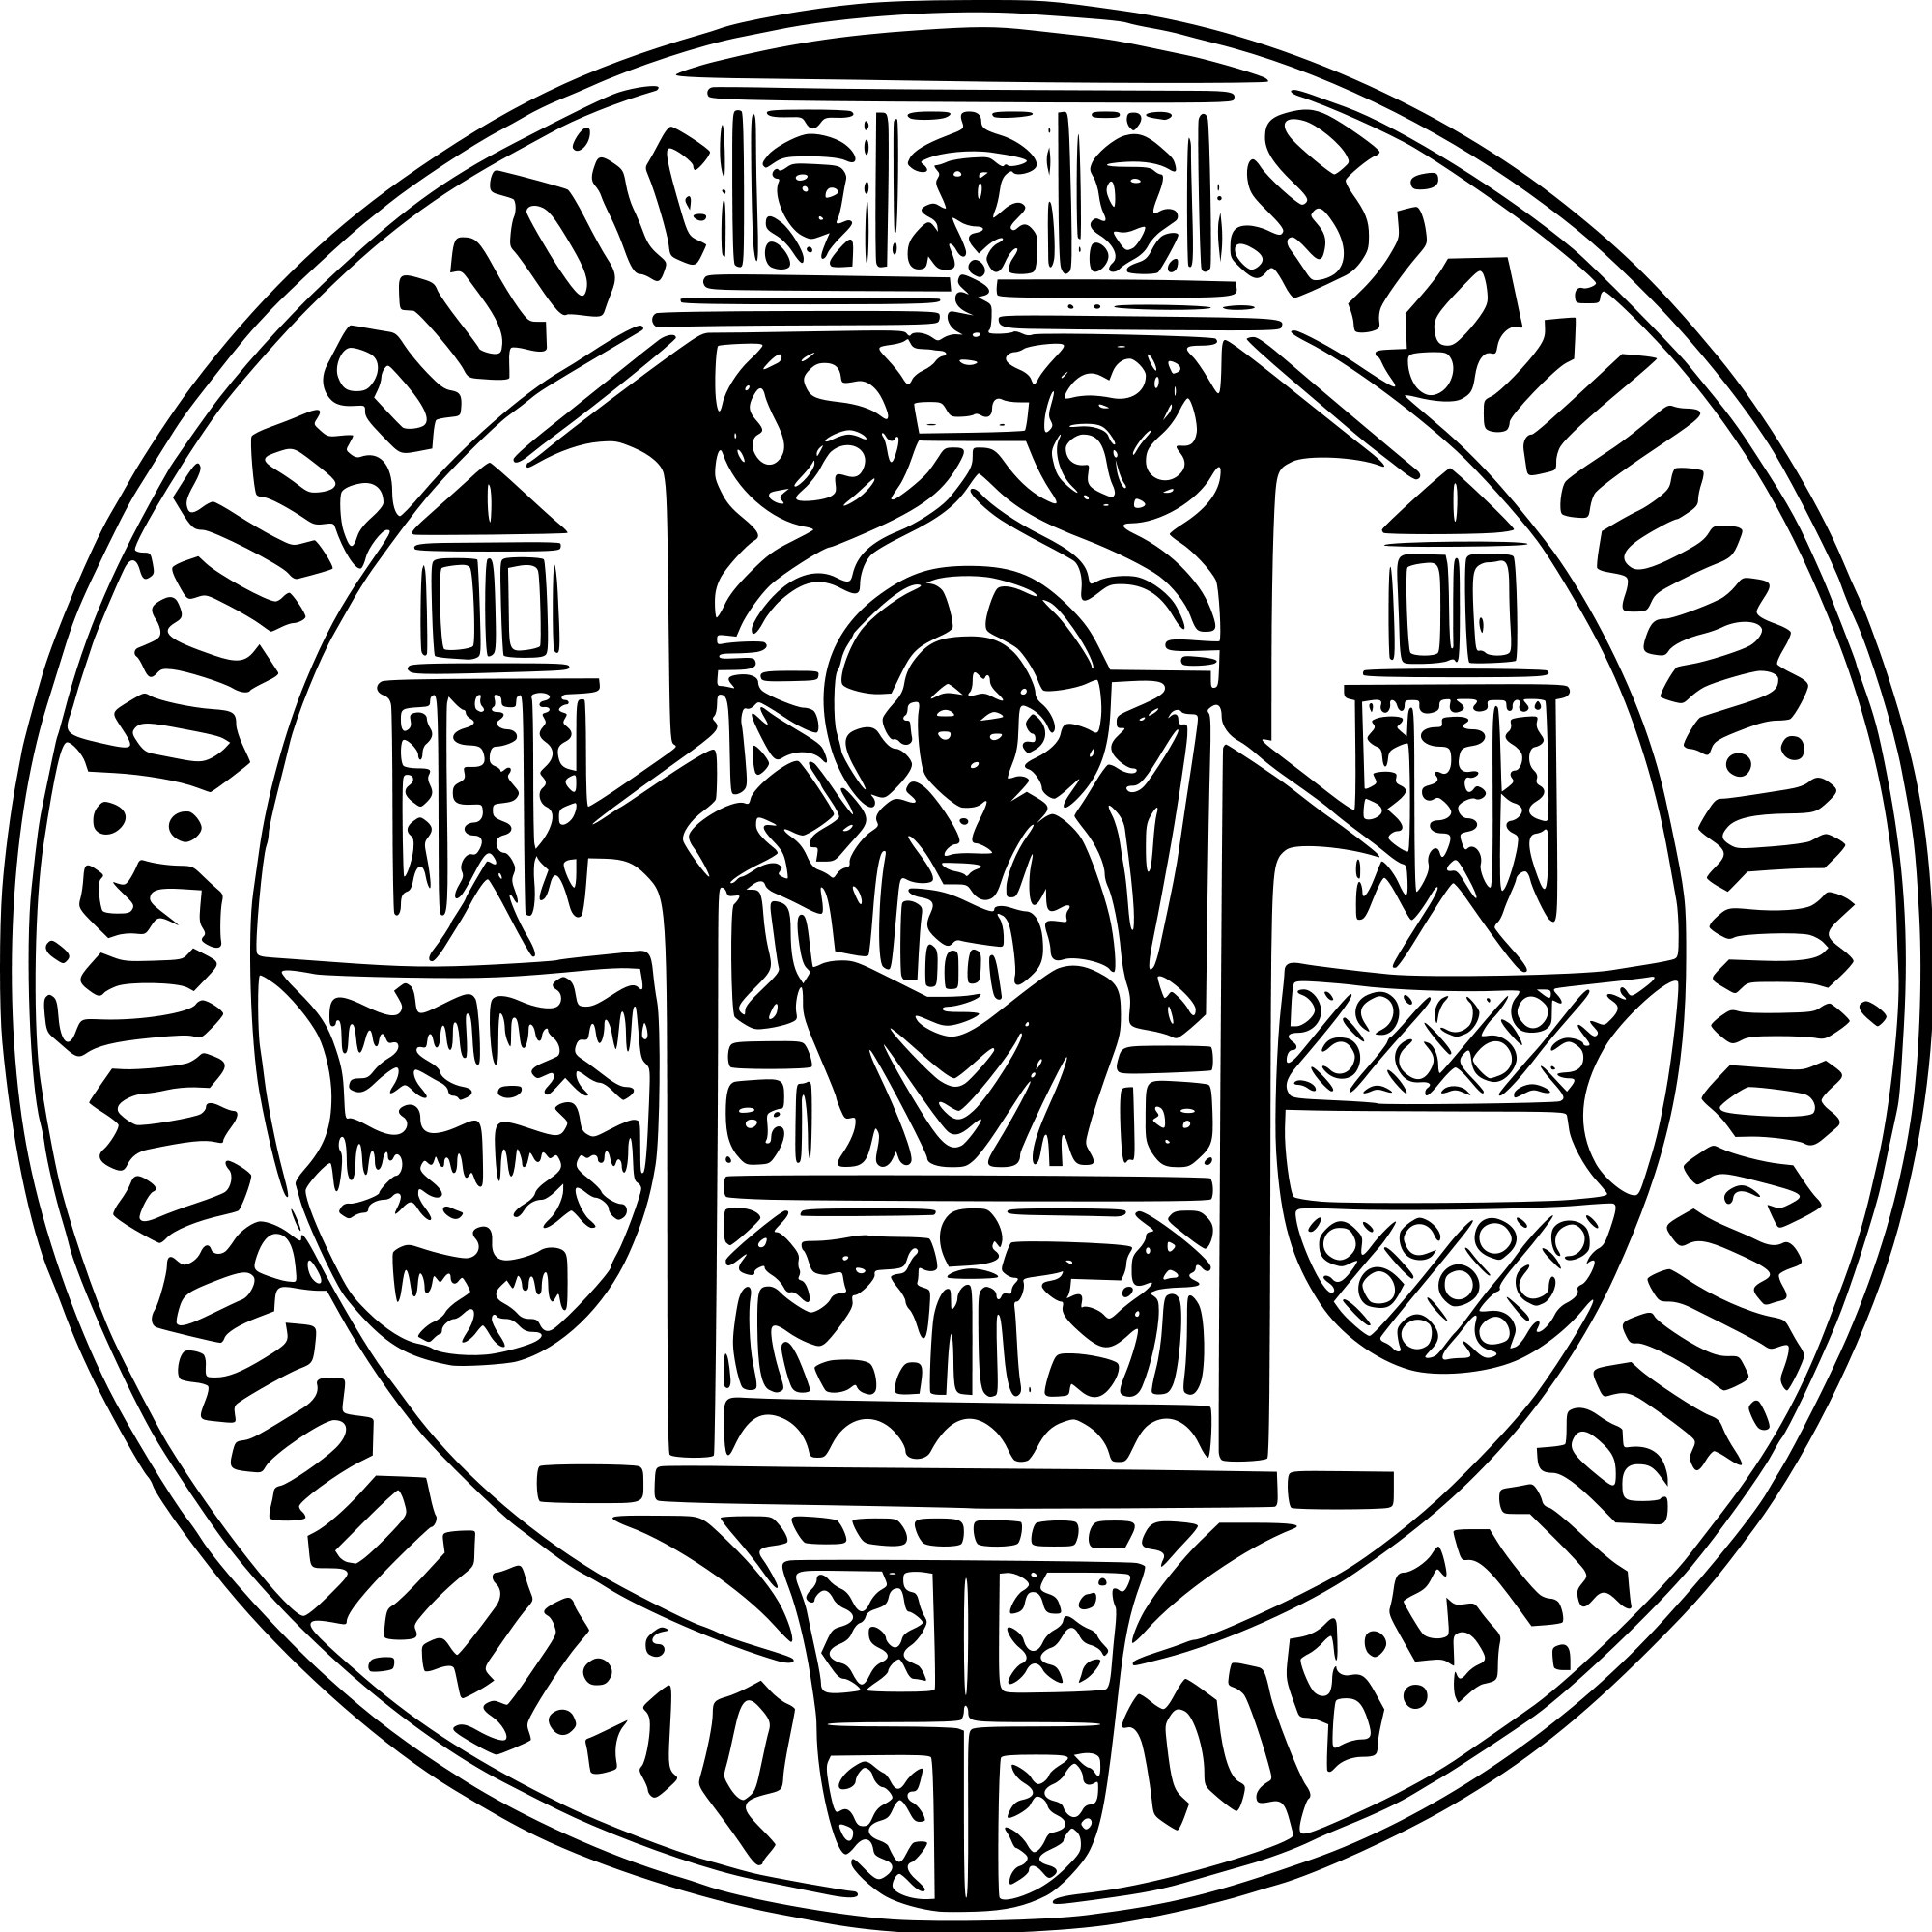
\includegraphics[width=0.5\textwidth]{Figures/Siegel.png} 
\\[1.3cm]

%\textsc{\LARGE \univname}\\[1.5cm] % University name
%\textsc{\Large Doctoral Thesis}\\[0.5cm] % Thesis type

%\HRule \\[0.4cm] % Horizontal line
{\huge \textbf{Bioinformatic analyses of\\MOF-containing complexes\\[9pt]in mammals and \textit{Drosophila}}}\\[1.5cm] % Thesis title
%\HRule \\[1.5cm] % Horizontal line


\textsc{\LARGE Inaugural-Dissertation}\\[1cm] % University name
\large zur Erlangung der Doktorwürde\\der Fakultät für Biologie\\der Albert-Ludwigs-Universität Freiburg im Breisgau\\[1cm] % University requirement text
 % Author name - remove the \href bracket to remove the link

\large vorgelegt von\\Friederike Dündar \\[1.5cm]
 
\large Freiburg im Breisgau \\ Oktober 2014 \\ % Date

\vfill
\end{center}

\end{titlepage}

%----------------------------------------------------------------------------------------
%	DECLARATION PAGE
%	Your institution may give you a different text to place here
%----------------------------------------------------------------------------------------

%\Declaration{

%\addtocontents{toc}{\vspace{1em}} % Add a gap in the Contents, for aesthetics

%I, \authornames, declare that this thesis titled, '\ttitle' and the work presented in it are my own. I confirm that:

%\begin{itemize} 
%\item[\tiny{$\blacksquare$}] This work was done wholly or mainly while in candidature for a research degree at this University.
%\item[\tiny{$\blacksquare$}] Where any part of this thesis has previously been submitted for a degree or any other qualification at this University or any other institution, this has been clearly stated.
%\item[\tiny{$\blacksquare$}] Where I have consulted the published work of others, this is always clearly attributed.
%\item[\tiny{$\blacksquare$}] Where I have quoted from the work of others, the source is always given. With the exception of such quotations, this thesis is entirely my own work.
%\item[\tiny{$\blacksquare$}] I have acknowledged all main sources of help.
%\item[\tiny{$\blacksquare$}] Where the thesis is based on work done by myself jointly with others, I have made clear exactly what was done by others and what I have contributed myself.\\
%\end{itemize}
\thispagestyle{empty}
\vspace*{\fill}
Dekan der Fakultät für Biologie: Prof. Dr. Wolfgang Driever \\
Promotionsvorsitzender: Prof. Dr. Stefan Rotter \\
Betreuer der Arbeit: Dr. Asifa Akhtar \\
Referent: Dr. Asifa Akhtar \\
Koreferent: Prof. Dr. Wolfgang Hess \\
Drittprüfer: Prof. Dr. Jörn Dengjel\\
Datum der mündlichen Prüfung:
\clearpage
%Signed:\\
%\rule[1em]{25em}{0.5pt} % This prints a line for the signature
 
%Date:\\
%\rule[1em]{25em}{0.5pt} % This prints a line to write the date
%}

%\clearpage % Start a new page
%----------------------------------------------------------------------------------------
%	ACKNOWLEDGEMENTS
%----------------------------------------------------------------------------------------

\setstretch{1.3} % Reset the line-spacing to 1.3 for body text (if it has changed)
\acknowledgements{ % Add a gap in the Contents, for aesthetics \addtocontents{toc}{\vspace{1em}}
%\pagenumbering{roman}
\thispagestyle{empty}
I cannot imagine a place where I would have rather spent my PhD years than the MPI-IE. Representatively, I would like to thank the entire Akhtar Group, the Bioinformatics Group and the Deep Sequencing Unit at the MPI-IE -- for endless, fruitful discussions about everything, and for being awesome peers! All my projects were collaborative projects in the best sense and none of them would have been accomplished without the work and insights from everyone involved.

I am especially indebted to:

\textbf{Asifa} who had so much faith in my abilities that did not even exist at the beginning of my PhD, gave me all the support and freedom that I needed to find my way into the bioinformatics community, inspired and motivated me without end with her enthusiasm.
\textbf{Fidel} who first helped me lose my feaR and then pushed me towards python, eagerly discussed tedious problems and details, enabled me (and many others) to do analyses faster and more impressively than I would have ever imagined, always takes initiative and seeks solutions rather than work-arounds, and makes the most delicious veggie sticks.
\textbf{Ken} who introduced me to ChIP-seq analysis, the NSL complex and everything else I needed to know, who never ran out of sharp insights, clever questions and new analyses and who truly impressed me with his honest passion for science. I don't know if I had ever become a computational biologist without his help and inspiration.
\textbf{Sarah} who painlessly introduced me to the UNIX shell and scripting, installed countless stubborn programs, sat with me for hours hunting other people's code bugs, masters the Galaxy, tames the servers and tirelessly fights back the rising chaos of increasing data and people messing with it, and, most importantly, selflessly ensures a constant supply of Luxemburgian coffee pads.
\textbf{Thomas} who let me become part of the bioinformatics group despite my utter lack of bioinformatics savvy in the beginning, whose support I could always, always count on, whose one-on-one supervision was absolutely essential for the success of my very first bioinformatic steps and without whom I still would have never driven a go-kart.
\textbf{Tomek} who trusted me with his data, was a constant source of inspiring ideas, made the most beautiful illustrations and always brought exquisite delicacies from Poland and Paris.

I would also like to thank Andrew Pospisilik and Michael Stadler who supported me during TAC meetings and beyond. I couldn't have had a better TAC!
}
%\clearpage % Start a new page



%----------------------------------------------------------------------------------------
%	LIST OF CONTENTS/FIGURES/TABLES PAGES
%----------------------------------------------------------------------------------------

\pagestyle{fancy} % The page style headers have been "empty" all this time, now use the "fancy" headers as defined before to bring them back
\pagenumbering{roman}
%\lhead{\emph{Contents}} % Set the left side page header to "Contents"
\fancyhead[RO,LE]{\emph{Contents}}
\fancyfoot{}

\tableofcontents % Write out the Table of Contents

%\lhead{\emph{List of Figures}} % Set the left side page header to "List of Figures"
\fancyhead[RO,LE]{\emph{List of Figures}}
\fancyfoot{}

\listoffigures % Write out the List of Figures

%\lhead{\emph{List of Tables}} % Set the left side page header to "List of Tables"
\fancyhead[RO,LE]{\emph{List of Tables}}
\fancyfoot{}
\listoftables % Write out the List of Tables

%%-----------------------------
\setstretch{1.3}  % Set the line spacing to 1.5, this makes the following tables easier to read
%\clearpage  % Start a new page
%\lhead{\emph{Abbreviations}}  % Set the left side page header to "Abbreviations"
\fancyhead[RO,LE]{\emph{Abbreviations}}
\fancyfoot{}
\listofsymbols{ll}  % Include a list of Abbreviations (a table of two columns)
{
%\begin{table}[h]
%\begin{tabular}{rl}
%\centering
ac          & acetylation                                   \\
AT          & adenine, thymine                              \\
ATP         & adenosine triphosphate                        \\
bp          & base pair                                     \\
ChIP        & chromatin immunoprecipitation                 \\
CTD         & C-terminal domain                             \\
D., d          & \textit{Drosophila}                         \\
DNA         & deoxyribonucleic acid                         \\
ESC         & embryonic stem cell                           \\
G2/M        & pre-mitotic phase to mitosis                 \\
GC          & dinucleotide: guanine, cytosine               \\
h           & human                                         \\
H2B, H3, H4 & histones 2B, 3, 4                             \\
HAT         & histone acetyl transferase                    \\
K           & lysine                                        \\
KAT         & lysine acetyl transferase                     \\
kb          & kilo base pair                                \\
KMT         & lysine methyl transferase                     \\
M., m          & \textit{Mus}, murine, mouse                               \\
me          & methylation                                   \\
modENCODE   & (model organism) encyclopedia of DNA elements \\
NAD         & nicotinamide adenine dinucleotide             \\
NPC         & neuronal progenitor cell                      \\
PCR         & polymerase chain reaction                     \\
PIC         & pre-initiation complex                        \\
Pol II      & RNA polymerase II                             \\
RNA         & ribonucleic acid                              \\
RNAi        & RNA interference                              \\
seq         & high-throughput DNA sequencing                \\
SES         & signal extraction scaling                     \\
shRNA       & small hairpin RNA                             \\
TES         & transcription end site                        \\
TF          & transcription factor                          \\
TSS         & trancription start site                       \\
ub          & ubiquitylation                                \\
UTR         & untranslated region                           
%\end{tabular}
%\end{table}

% \textbf{Acronym} & \textbf{W}hat (it) \textbf{S}tands \textbf{F}or \\
%\textbf{LAH} & \textbf{L}ist \textbf{A}bbreviations \textbf{H}ere \\
}
%% ----------------------------------------------------------------
% End of the pre-amble, contents and lists of things
% Begin the Dedication page

\setstretch{1.3}  % Return the line spacing back to 1.3

%\pagestyle{empty}  % Page style needs to be empty for this page
%\dedicatory{For/Dedicated to/To my\ldots}

\addtocontents{toc}{\vspace{2em}}  % Add a gap in the Contents, for aesthetics

%----------------------------------------------------------------------------------------
%	THESIS CONTENT - CHAPTERS
%----------------------------------------------------------------------------------------

\mainmatter % Begin numeric (1,2,3...) page numbering

\pagestyle{fancy} % Return the page headers back to the "fancy" style
\setstretch{1.3}
% Include the chapters of the thesis as separate files from the Chapters folder
% Chapter Template

\chapter{Summary} % Main chapter title

\label{Abstract} % for referencing this chapter elsewhere, use \ref{ChapterX}

%\lhead{Summary} % this is for the header on each page - perhaps a shortened title
\fancyhead[RO,LE]{Summary}
\fancyfoot[C]{\thepage}

\section{Zusammenfassung}

%Differenzielle Genexprimierung bildet die Grundlage für die Möglichkeit zur Ausbildung verschiedener Zellidentitäten und Verhaltensmuster. Chromatin spielt hierbei eine wichtig Rolle, da es vielfach modifiziert werden kann und direkten Einfluss auf die Genaktivität hat.
Die Histon-Acetyltransferase MOF (males absent on the first) ist das wichtigste Enzym für die Acetylierung von Lysin 16 des Histons H4, wobei die katalytische Spezifität und Effektivität stark von ihren Interaktionspartnern, den MSL (male-specific lethal) und NSL (non-specific lethal) Komplexen, bestimmt wird. Der MSL Komplex ist von herausragender Bedeutung in der Taufliege (\textit{D.~melanogaster}), wo er für die transkriptionelle Kompensation der reduzierten Gendosis in X-chromosomal hemizygoten \textit{Drosophila}-Männchen verantwortlich ist. Welche Funktionen der MSL Komplex in Säugetieren erfüllen könnte, war zu Beginn meiner Arbeit kaum bekannt, ebensowenig wie die Rolle des NSL Komplexes, welcher weder in der Fliege noch in Säugetieren umfänglich erforscht war. Das Ziel meines Projekts war es, unser Wissen über beide MOF-Komplexe deutlich zu erweitern.

Die Grundlage meiner Arbeit bildeten Chromatin-Im\-mun\-prä\-zi\-pi\-ta\-tions\-ex\-pe\-ri\-men\-te ge\-folgt von Hoch\-durch\-satz-DNA-Se\-quen\-zierung (ChIP-seq) für deren bio\-in\-for\-ma\-tische Analyse zu\-nächst standardisierte Protokolle sowie individuelle Auswertungen etabliert werden mussten. Das daraus resultierende Software-Paket deepTools kann nun für Qualitätskontrollen, Normalisierungen und Datenprozessierung ebenso verwendet werden wie für die bildliche Darstellung der Hoch\-durch\-satz-DNA-Se\-quen\-zierungs\-daten.

Wir untersuchten die genomweiten Bindestellen des NSL Komplexes in \textit{Drosophila}- (NSL1, NSL3, MCRS2, MBD-R2) und Mauszellen (NSL3, MCRS1) und konnten mittels umfangreicher Charakterisierung der Zielgene und RNAi-basierten Experimenten zeigen, dass
der NSL Komplex für die Ex\-pri\-mierung konstitutiv aktiver Gene vonnöten ist, um u.a. eine ausreichende Rekrutierung der RNA Polymerase II innerhalb des Prä\-ini\-tia\-tions\-kom\-plexes zu garantieren.

Zusätzlich zum NSL Komplex untersuchten wir auch MOF und den MSL Komplex (MSL1, MSL2) in Mauszellen. In der überwiegenden Mehrzahl der Promoterbindestellen fanden wir MOF gemeinsam mit dem NSL Komplex vor, in einigen Fällen lag zusätzlich ein Signale des MSL Komplexes vor. Obwohl der MSL Komplex -- anders als in der Taufliege -- in Mauszellen keine starke Präferenz für das X Chromosom zeigt, stellten sich MSL1 und MSL2 als essentiell für den Erhalt der X-chromosomalen Genexprimierung in embryonalen Stammzellen heraus, da in ihrer Abwesenheit die Transkription von \textit{Tsix} und die damit verbundene Produktionshemmung der X-inaktivierenden \textit{Xist}-RNA stark beeinträchtigt ist. Der NSL Komplex trägt indirekt zur Inhibierung der X-Inaktivierung bei, indem er für die Exprimierung von Pluripotenzfaktoren wie Nanog, Oct4 und Esrrb in embryonalen Stammzellen erfoderlich ist. Darüber hinaus verglichen wir die genomweiten Signale von MSL1 in evolutionär weit voneinander entfernten Spezies (\textit{D.~melanogaster, D.~virilis} und \textit{M.~musculus}), aus welchen wir schlussfolgerten, dass MSL1 geschlechtsunabhängig an Genpromotoren bindet -- anders als bislang angenommen, auch in \textit{D.~melanogaster}.

Zusammenfassend konnten wir zeigen, dass die mit MOF interagierenden Proteinkomplexe zum Teil deutlich voneinander abgrenzbare Funktionen ausführen: während der NSL Komplex in großem Ausmaß die grundlegende Exprimierung von basalen Haushaltsgenen reguliert, ist der MSL Komplex an hoch spezialisierten, aber ebenfalls lebenswichtigen Prozessen beteiligt.


\section{Abstract}

%Chromatin-related processes are important for differential gene regulation which is the basis for cell fate and behavior.
The histone acetyl transferase males absent on the first (MOF) is responsible for the majority of histone H4 lysine 16 acetylation in \textit{Drosophila} and mammals. Its catalytic specificity and efficiency depend on the interaction with two protein complexes, the male-specific lethal (MSL) complex and the non-specific lethal (NSL) complex. The \textit{Drosophila} MSL complex has been thoroughly examined as it is essential for the transcriptional upregulation of the single male \textit{Drosophila} X chromosome to meet autosomal gene expression levels. Its function in mammals, however, was not clear. Likewise, the role of the NSL complex was poorly understood in both \textit{Drosophila} and mammalian cells. The aim of my project was to further our insights into these two distinct MOF-associated complexes.

All studies presented here were centered around chromatin immunoprecipitation experiments followed by high-throughput DNA sequencing (ChIP-seq). The analyses required the set-up of a universal bioinformatic pipeline and customized workflows for downstream analyses and visualizations. These efforts became part of the deepTools software package that allows efficient and reproducible generation of normalized coverage files, offers quality controls and highly customizable visualization of high-throughput sequencing data.

By investigating the genome-wide binding of NSL complex members in \textit{Drosophila} (NSL1, NSL3, MCRS2, MBD-R2) and mouse cells (NSL3, MCRS1) and subsequent extensive characterization of target genes coupled with perturbation experiments, we revealed that the NSL complex is an evolutionarily conserved regulator of housekeeping gene expression that is required for optimal recruitment of the pre-initiation complex. 

In mammals, we complemented our study of the NSL complex with genome-wide profiles of MOF, MSL1 and MSL2 in murine embryonic stem cells (ESC) and neuronal progenitor cells (NPC). We determined constant and dynamic binding during differentiation and established the patterns of exclusive and concomitant targeting of both MOF-associated complexes. We found that the NSL complex is the predominant interaction partner of MOF in ESCs and NPCs. While the MSL complex is not specifically enriched on the mouse X chromosome, we could show that MSL1 and MSL2 are important for the maintenance of active X expression in ESCs by maintaining transcription of \textit{Tsix} whose expression inhibits the production of the X-inactivating transcript, \textit{Xist}. The NSL complex indirectly contributes to the repression of X inactivation through expression regulation of key pluripotency factors such as Nanog, Oct4 and Esrrb. Furthermore, the role of MSL1 was elucidated in more detail as the genome-wide profiles from distant species (\textit{D.~melanogaster, D.~virilis} and \textit{M.~musculus}) revealed evolutionarily conserved binding to gene promoters in a sex-independent manner. 

In summary, we could show that MOF-associated complexes fulfill distinct vital roles in \textit{Drosophila} and mammals: while the NSL complex is an abundant regulator of basic cellular gene expression, the MSL complex was found to contribute to highly specialized functions.



\chapter{Introduction} % Main chapter title

\label{Body} % for referencing this chapter elsewhere, use \ref{ChapterX}

%\lhead{Introduction} % this is for the header on each page - perhaps a shortened title
\fancyhead[RO,LE]{Introduction} % puts the chapter title on the left for odd pages, on the right for even pages
\fancyfoot[C]{\thepage}

Living cells constantly need to monitor their own status as well as their environment while maintaining the means to absorb and utilize energy. The majority of these functions is carried out by a vastly diverse set of amino-acid-based macromolecules which were termed proteins (from the Greek word \textit{proteios} for ``being of the first order'') to indicate their ubiquitous presence in all organisms \citep{Vickery1950}. The construction plans for all the proteins of an organism are stored in another biological macromolecule, deoxyribonucleic acid (DNA), that is made up of two different purine-pyrimidine base pairs chained together by sugar-phosphate bonds. The four bases adenosine, cytosine, guanine and thymine (A, C, G, T) form the genetic code that determines the order of amino acids for every protein a cell can make \citep{Campbell2003}.

%%%%%%%%%%%%%%%%%%%%%%
%%% Figure Gene Expression 
\begin{figure}[htb]
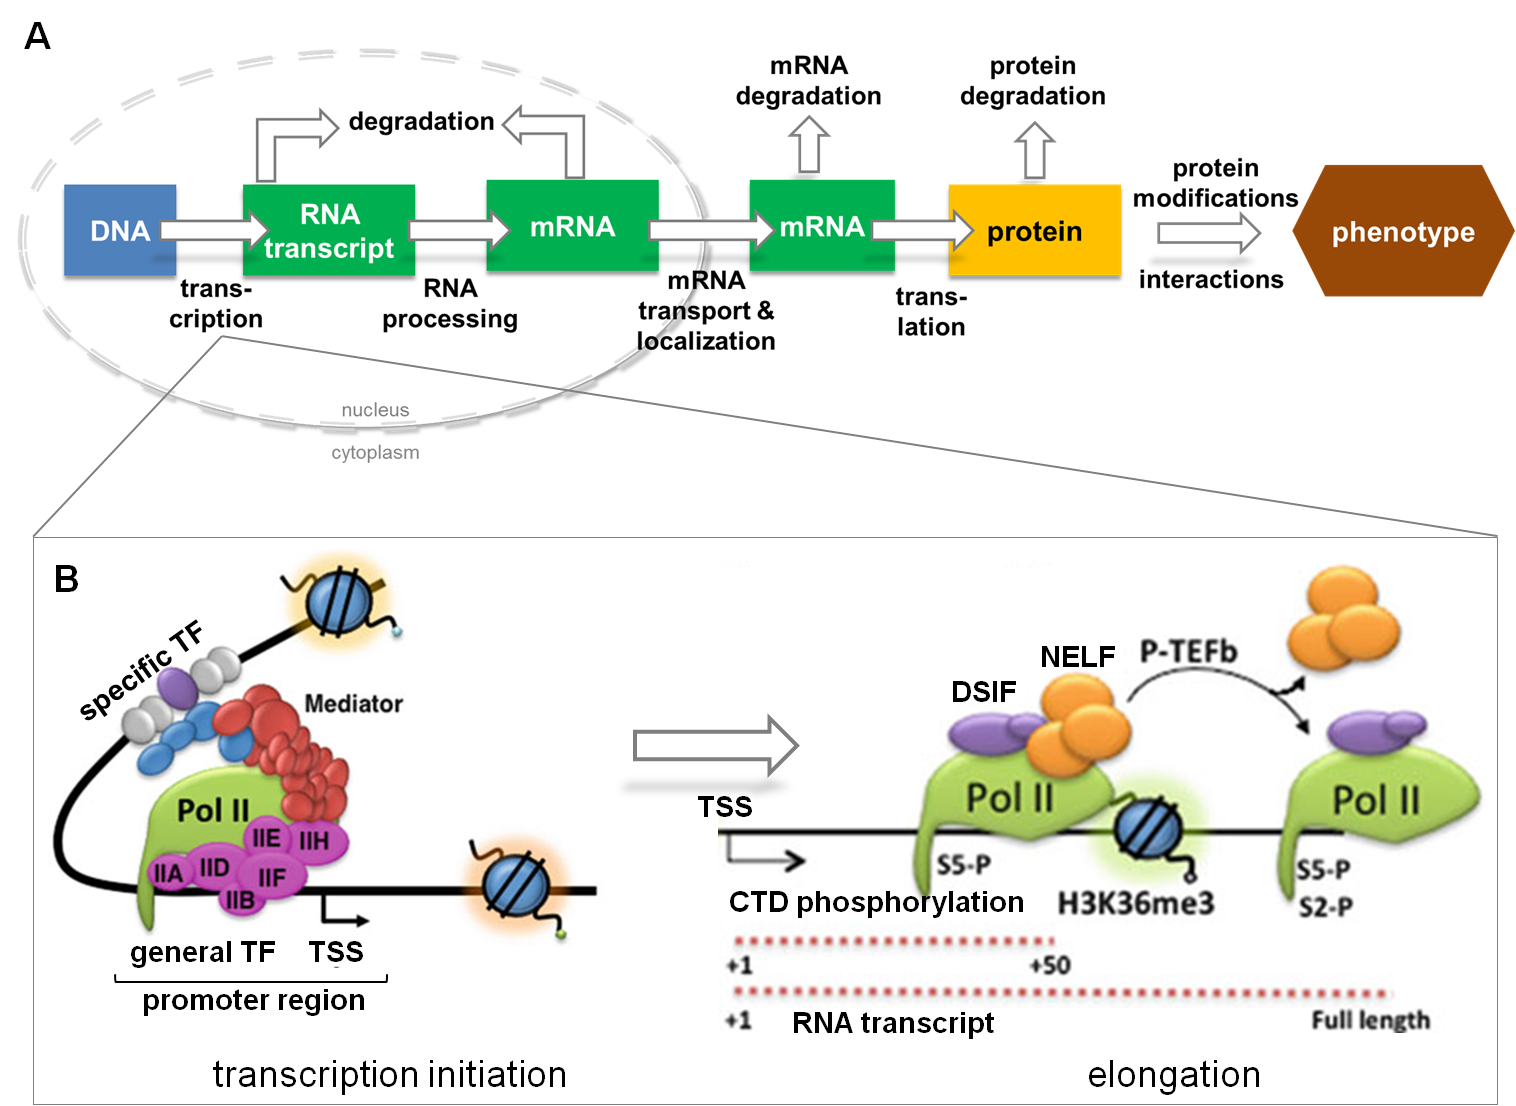
\includegraphics[width=1\textwidth,trim=2 0 2 2,clip]{Figures/CentralDogma.png}
\begin{footnotesize}
\caption[The multiple steps of gene expression in eukaryotes.]{\textsf{Gene expression -- the process of generating a protein based on the genetic code -- is a multi-step process.
\textbf{A)} Proteins are the main effector molecules for the phenotype of a cell. DNA-encoded genes are copied into RNA that needs to be processed and exported out of the nucleus into the cytoplasm where the translation of the nucleic acid code into the primary amino acid sequence of a protein takes place. The concept of this image was taken from \citet{Alberts2002}
\textbf{B)} In eukaryotes, the copying of protein-encoding genes into RNA templates is performed by the RNA Polymerase complex~II (Pol~II) whose action depends on manifold additional proteins. Specific transcription factors (TFs) bind to regulatory DNA regions close to the transcription start site (TSS, promoters) or further away (enhancers) where they i.a. initiate the remodelling of the chromatin to allow for Pol~II recruitment. The Mediator complex (shown in red) connects the TFs’ activation stimulus with Pol~II by direct physical interactions and it is essential for the assembly of the pre-initiation complex that entails Pol~II and general transcription factors (GTF, shown in pink). Subsequently, the DNA double-helix is unwound and RNA polymerization is initiated, marked by the phosphorylation of serine 5 (S5-P) of Pol~II’s C-terminal repeat domain (CTD). For the entire gene’s transcription to occur, elongation factors such as the positive transcription elongation factor b (P-TEFb) must replace the GTFs to release the negative elongation factor (NELF) and stimulate phosphorylation of serine 2 (S2-P) of the CTD. The two parts of this image and information conveyed here were taken from \citet{Barrero2013}.
}}
\label{fig:Expression}
\end{footnotesize}
\end{figure}
%%%%%%%%%%%%%%%%%%%%%%%%%%%

Not all of the proteins are needed in the same amount or at the same time as many proteins fulfill highly specialized functions, for example in response to environmental stress or developmental cues. Moreover, multi-cellular organisms contain cells with drastically different appearances and functions even though they all share the same genetic information. This wide range of distinct spatio-temporal phenotypes is based on the ability of the individual cells to read (express) those parts of the DNA that they need and to regulate the outcome quantitatively. As shown in \fref{fig:Expression}, gene expression is a multi-step process that includes the generation of a ribonucleic acid (RNA) copy, its processing, transport and subsequent translation into a primary amino acid chain that will eventually give rise to a protein. Each step can be influenced and modulated by regulatory mechanisms, but recent reports indicate that the beginning -- transcription -- is the major means for determining the final protein levels (it is estimated that up to 80\% of differences in individual protein abundance are explained solely by differences in transcription \citep{Li2014}).
%===================================================================
%	SECTION 
%===================================================================
\section{Transcription in eukaryotes}
Transcription itself is carried out by large protein complexes, most notably RNA Polymerase~II (Pol~II) that binds to the beginning of genes (promoters) and subsequently produces an RNA copy of the gene. In eukaryotes, i.e. organisms whose cells contain several membrane-enclosed organelles such as the DNA-containing nucleus \citep{Campbell2003b}, Pol~II does not have high intrinsic affinity for DNA binding. Therefore, protein-protein interactions that promote and stabilize the Pol~II-DNA interaction are essential for eukaryotic transcription \citep{Genomes2002}. Transcription regulation by so-called transcription factors can occur via binding to promoters or TSS-distal regulatory elements (enhancers) that contribute to the initiation of gene expression (see \fref{fig:Expression} for details). Furthermore, transcription factors themselves can be regulated through various means, e.g. by interactions with other proteins and small molecules, post-translational modifications or by changes of their own expression and degradation. 
%
\subsection{Chromatin and transcription}
In recent years, an additional layer of gene expression regulation has emerged: the packaging of the DNA. In the nuclei of eukaryotes, the DNA strand is generally not readily accessible as it is stored within a compact DNA-protein polymer, termed chromatin. Chromatin is made up of nucleosomes that are composed of protein octamers of four basic, evolutionarily extremely well conserved histone proteins with DNA wrapped around them (approximately 150 nucleotides per nucleosome, \fref{fig:histone}). This enables tremendous compaction of the long DNA strand \citep{Woodcock2010}, but it also offers more possibilities for gene expression regulation because nucleosomes sterically hinder transcription and need to be moved before transcription can occur. In fact, chromatin has emerged as a well-suited template for both dynamic, gene-specific effects as well as stable, continuously propagated changes of transcription that persist without changes of the DNA sequence (herein referred to as epigenetics).
%
%%%%%%%%%%%%
%%% Figure Histones/Nucleosomes 
\begin{figure}
 \begin{minipage}[c]{0.55\textwidth}
   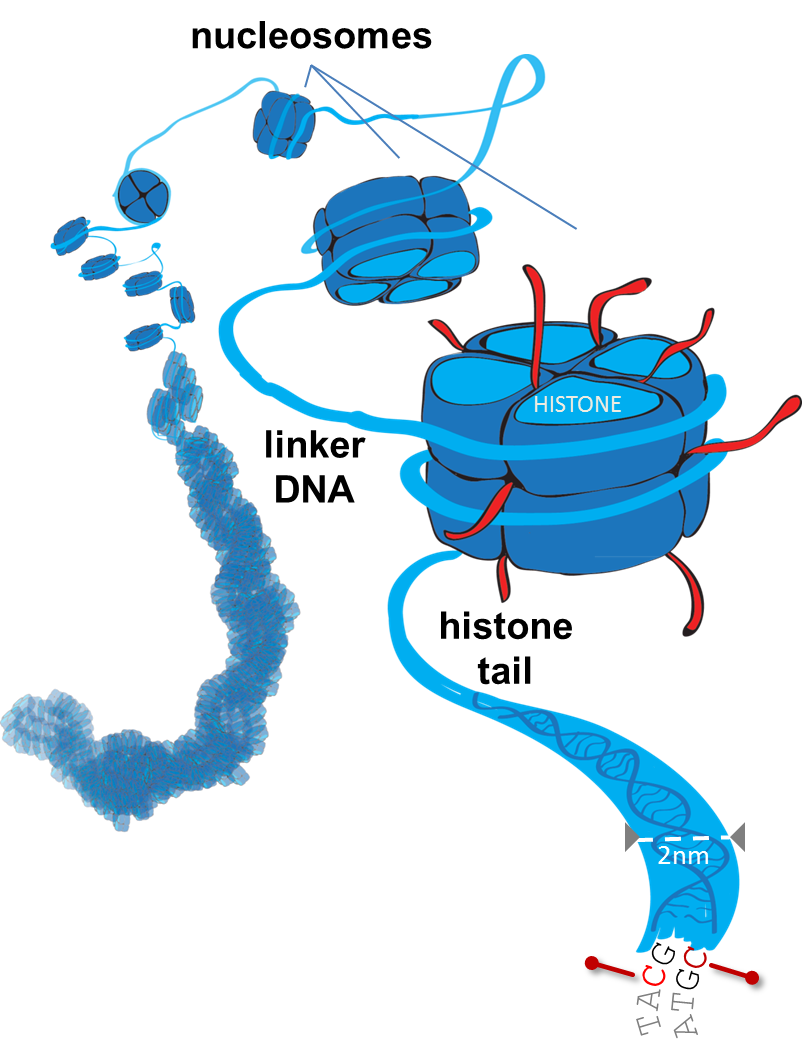
\includegraphics[width=\textwidth]{Figures/histones.png}
 \end{minipage}\hfill
 \begin{minipage}[c]{0.4\textwidth}
	\begin{footnotesize}
   \caption[Chromatin, the DNA-protein polymer of eukaryotic cells.]{\textsf{In eukaryotic cells, the DNA strand is wrapped around so-called nucleosomes -- octamers of the core histone proteins H2A, H2B, H3, H4. The linker DNA between nucleosomes can vary in length (7-100~bp) and is associated with histone H1 (not shown). Nucleosomes are transcription inhibitors as they restrict access to genes, but they can be influenced by physical force and post-translational modifications. The red strands indicate the N-terminal ends of the histones that protrude from the nucleosome and serve as substrates for myriad modifications \citep{Kouzarides2007} (\fref{fig:histonesExtended}). An additional epigenetic modification that does not alter the DNA code, but influences gene expression, is methylation of cytosines of CpG dinucleotides (red marker on the bottom) that is generally associated with silenced genes. The original image was taken from \citep{Histones} and modified by Tomasz Chelmicki and myself.
}}
\label{fig:histone}
\end{footnotesize}
 \end{minipage}
\end{figure}
%%%%%%%%%%%%%%%%%
%---------------------------------------
%%% Figure histone modifications
\begin{figure}
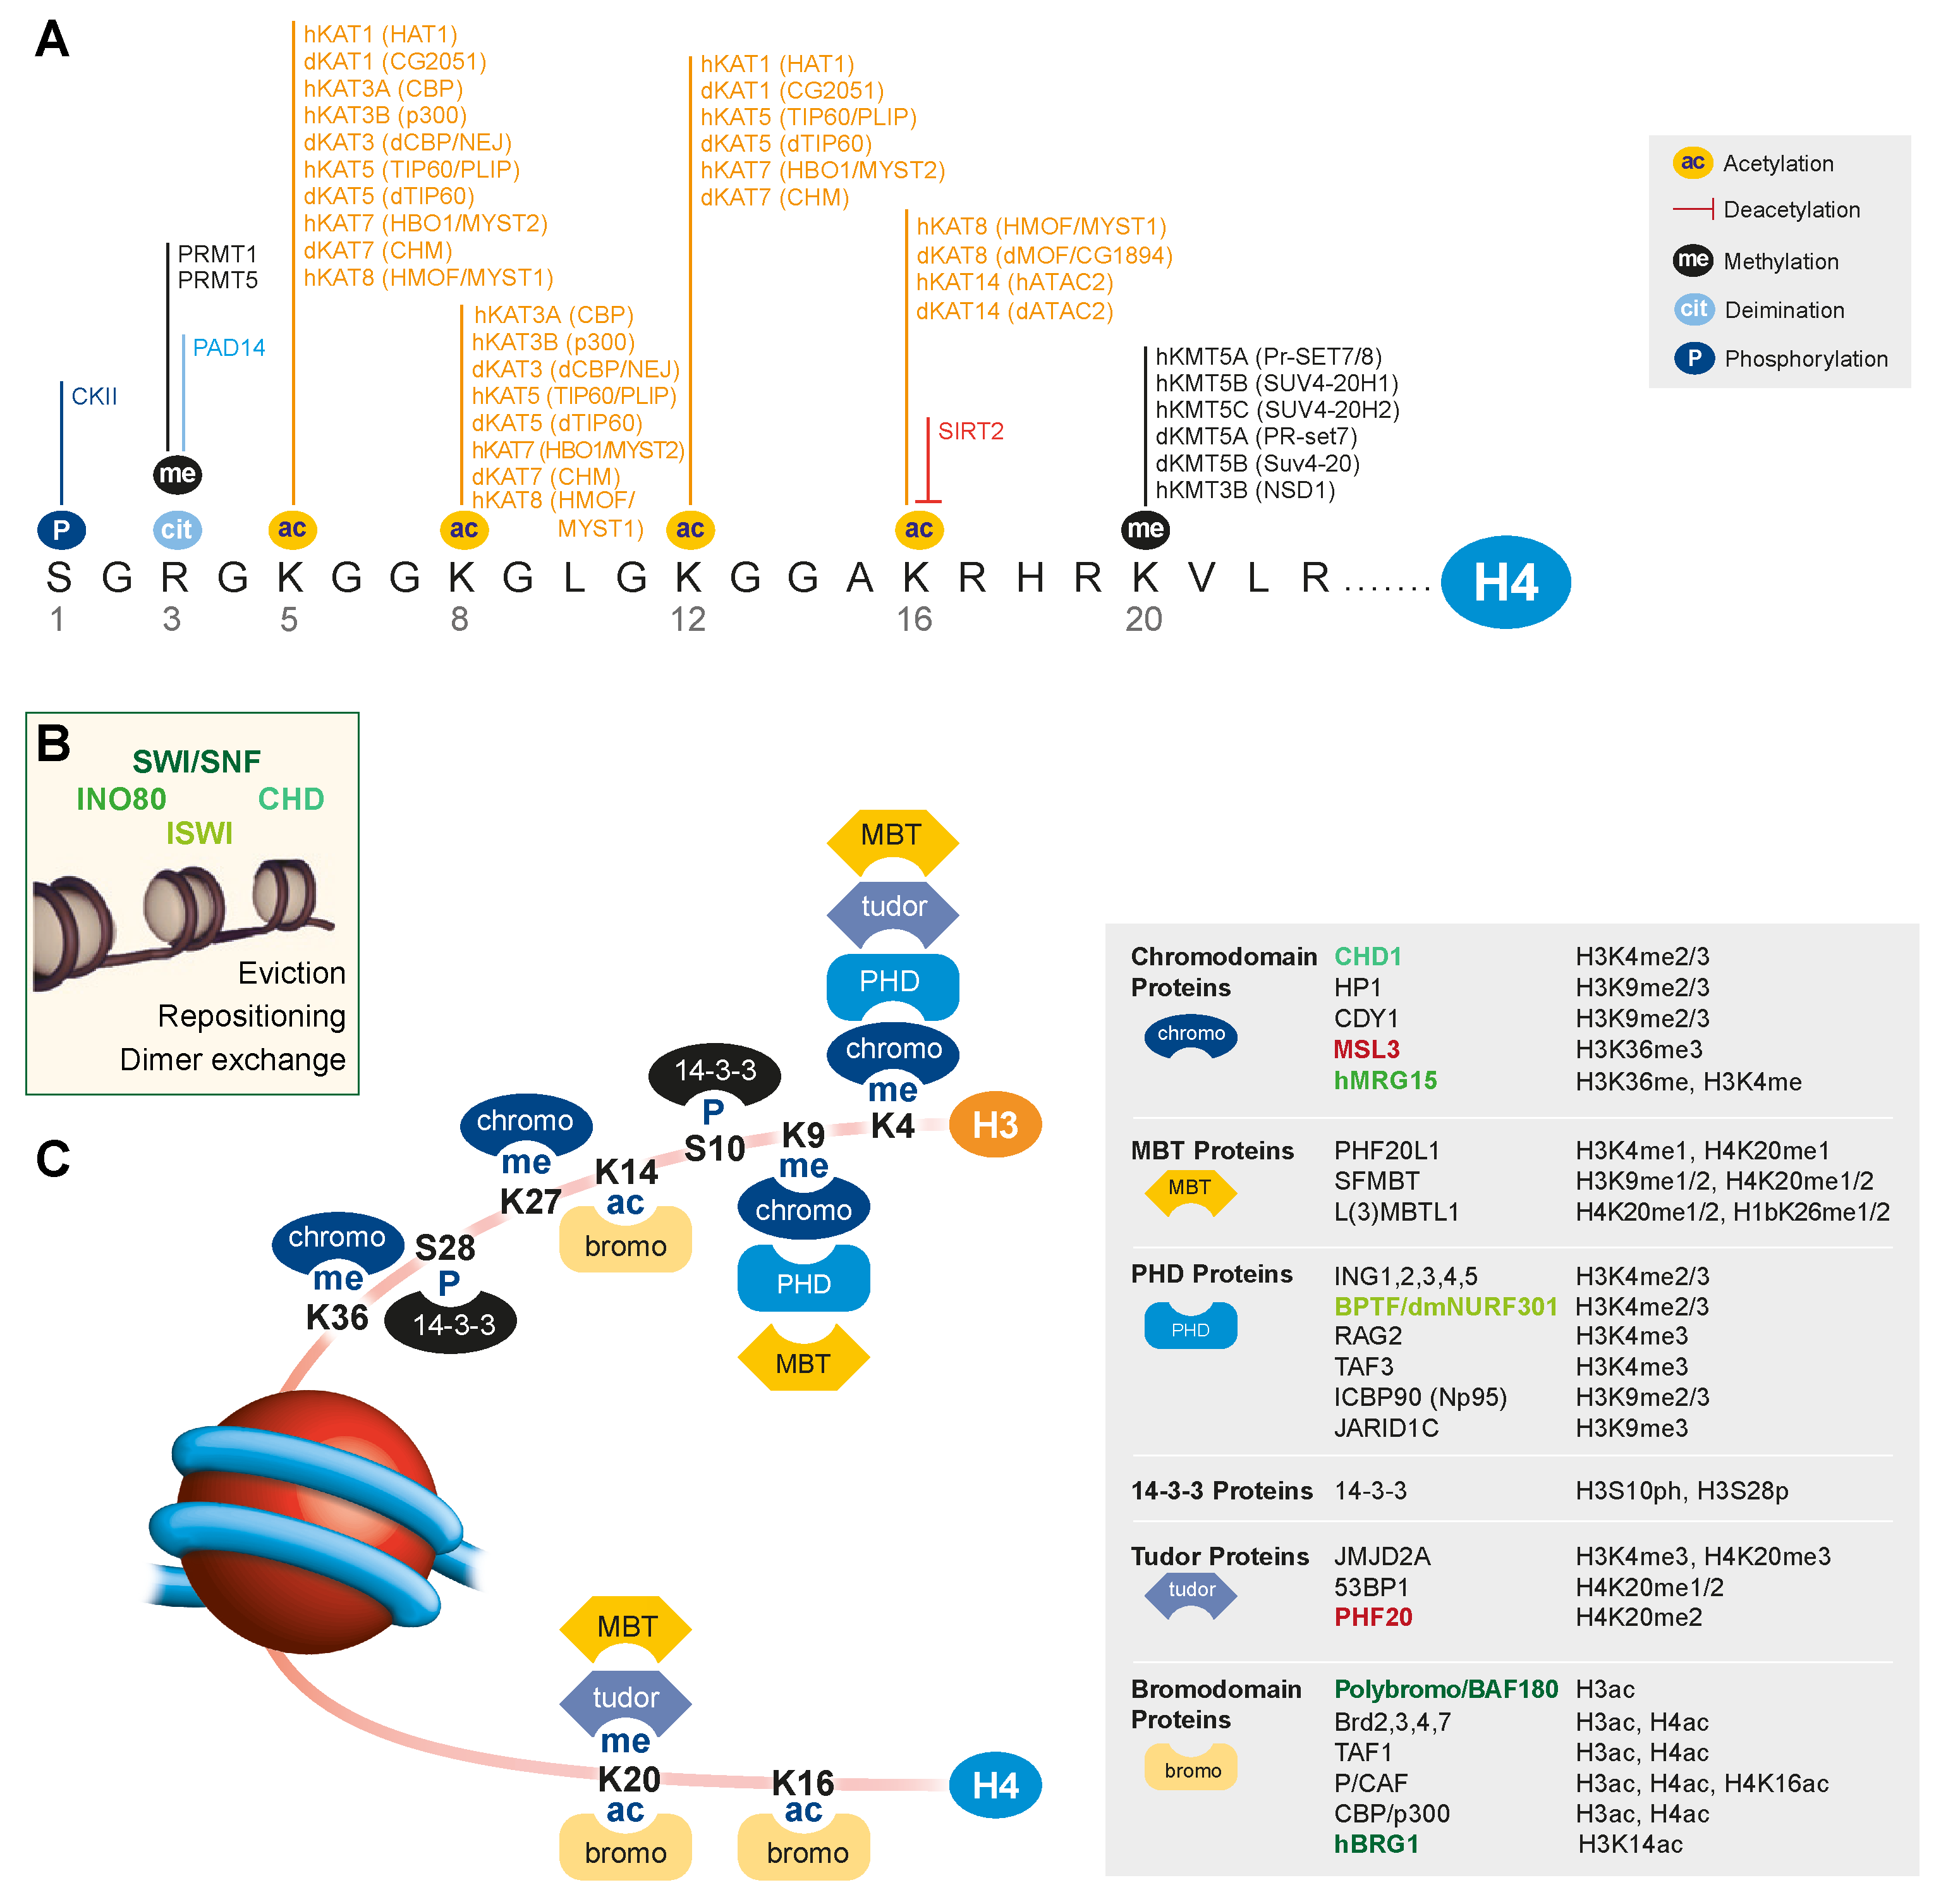
\includegraphics[width=1\textwidth]{Figures/histonesExtended.pdf}
\begin{footnotesize}
\caption[Exemplary histone modifications, their enzymes and histone-modification-recognizing protein domains.]{\textsf{Examples of histone modifications, corresponding enzymes and protein domains that recognize them.
\textbf{A)} Like for the other core histones, the tail of histone 4 (H4) contains numerous residues for covalent post-translational modifications of which some are shown here together with enzymes capable of catalyzing the respective mark in humans (h) and \textit{Drosophila} (d). Note that the different marks may have different biological meanings, e.g. methylation of H4K20 is associated with gene repression while acetylation of H4K16 is associated with gene activation (\fref{fig:histoneDistribution}). Moreover, the residues within the globular domains can also be modified (not shown). CKII = casein kinase II, PRMT = protein arginine methyltransferase, PAD2 = peptidyl arginine deiminiase, KAT = lysine acetyl transferase, KMT = lysine methyl transferase, SIRT2 = NAD-dependent deacetylase sirtuin-2. The image was taken from \citep{Abcam} and modified. See \tref{tab:HATs} for details on histone acetyl transferases.
\textbf{B)} Besides histone-modifying enzymes, chromatin remodellers greatly influence gene accessibility, too. There are four major families of ATP-dependent DNA translocases that can -- to varying degrees -- reposition, evict and replace nucleosomes. The INO80 family members are particularly important for DNA replication and repair as they can efficiently exchange histones while the multimeric complexes of the SWI/SNF family predominantly slide and evict nucleosomes \citep{Manelyte2013}.
\textbf{C)} Transcription factors (e.g. the transcription initiation factors TAF1 and 3), chromatin-remodelling complexes (shown in green, see B) and histone-modifying enzymes (e.g. the HATs CDY, p300 and P/CAF and the lysine demethylases JARID1C and JMJD2A) often contain domains that recognize specific histone modifications. Members of MOF-associated complexes are shown in red. The image was taken from \citep{Abcam} and modified.
}}
\label{fig:histonesExtended}
\end{footnotesize}
\end{figure}
%------------------------------------


%
The epigenetic influence on gene expression is based on two main properties of chromatin: its physical structure and the potential for myriad post-translational modifications of the histone residues of their N-terminal tails and globular domains (\fref{fig:histone}). The physical properties of nucleosomes can be altered by chromatin remodellers that apply a torsional strain to the DNA strand that generates enough force to change the position of a nucleosome \citep{Manelyte2013}. These ATP-dependent enzymes are required for the maintenance of active as well as silenced genome regions, they can replace the canonical core histones shown in \fref{fig:histone} with histone variants and they are required for the assembly of chromatin during DNA replication and DNA repair (reviewed by \citet{Manelyte2013}, see \fref{fig:histonesExtended} for the four families of chromatin remodellers).

Numerous histone-modifying enzymes are now known; they catalyze the transfer of small organic groups (e.g. methyl, acetyl and phosphate groups) or small proteins (e.g. ubiquitin) to histone residues, especially to their tail regions (\fref{fig:histonesExtended}). The tail domains of the histones are not essential for nucleosome formation, but their modifications contribute to the recruitment of chromatin- and DNA-binding proteins \citep{Turner2014} (see \fref{fig:histonesExtended} for histone binding domains) and serve as landmarks of active transcription (euchromatin) as well as silenced regions (heterochromatin). Although more than 100 histone modifications have been described \citep{Kouzarides2007, Tan2011} and well-defined histone mark combinations are the basis for distinct chromatin states associated with different levels of transcription \citep{Ernst2010,Kharchenko2011}  (see \fref{fig:histoneDistribution}), the debate about whether they are cause, consequence or merely a by-product of gene transcription is on-going \citep{Henikoff2011, Ptashne2013, Whitehouse2013}. On the other hand, the impact of chromatin structure on transcription is well established on at least two levels: high nucleosome density interferes with transcription factor binding and gene activation (reviewed by \citet{Henikoff2011}) and higher order chromatin domains separate euchromatin from heterochromatin, presumably to enable efficient transcription and constrain transcriptional inactivation \citep{Dixon2012}. Proteins that modify histones (e.g. methyl transferases, acetyl transferases) and ATP-dependent nucleosome remodellers have accordingly risen as a new class of transcription-related factors that do not necessarily need to directly interact with DNA to influence gene expression (\fref{fig:histonesExtended}).\\
%\begin{minipage}{\textwidth} % to avoid pagebreaks despite longtable environment
%\setlength{\extrarowheight}{2pt}
%\renewcommand{\arraystretch}{1.5}
\vspace*{-2em}
%\begin{longtable}[l]{>{\textsf\bgroup}p{3cm}<{\egroup} >{\textsf\bgroup}p{2.5cm}<{\egroup}>{\textsf\bgroup}p{5cm}<{\egroup}} % defining the columns - these must match the widths defined for the mini pages down below!
\begin{table}[t]
\begin{singlespacing}
\begin{small}
\begin{sffamily}
\caption[The main histone acetyl transferase families.]{\textsf{The main histone acetyl transferase families. The lysine acetyl transferase (KAT) designation indicates the standardized nomenclature suggested for HATs. GNAT = Gcn5-related \textsl{N}-acetyl transferase, MYST = MOZ, Ybf2/Sas3, Sas2, Tip60. The table was taken from \citet{Berndsen2008}}} %\\ % the \\ is important!
\label{tab:HATs}
\begin{tabular}{>{\small\textsf\bgroup}p{3.5cm}<{\egroup} >{\small\textsf\bgroup}p{3.5cm}<{\egroup} >{\small\textsf\bgroup}p{5cm}<{\egroup} }
%%%%%%%%%%%%%%%
% table title
\textbf{Enzyme} & \textbf{KAT designation} & \textbf{Histone specificity}
\tabularnewline \toprule
%-----------------------
\textbf{GNAT family} & & \\
Gcn5 & 2 & H3K9, 14, 36 \\
p/CAF & 2B & H3K14
\tabularnewline \midrule
%--------------------------
\textbf{MYST family} & & \\
Tip60 & 5 & H4K5, K8, K12 (K16) \\
MOF 	&	8	&	H4K5, K8, K16 \\
Sas3	&	6	&	H3K14, K23 \\
MOZ		&	6A & H3K14
\tabularnewline \midrule
%--------------------------
\textbf{p300 and others} & & \\
CBP & 3A & H2AK5, H2B \\
p300 	&	3B	&	H2AK5, H2B \\
Rtt109	&	11 & H3K56, K9, K23	
%--------------------------
\tabularnewline \bottomrule
%-----------------------------
\end{tabular}
%\label{tab:HATs}
%\end{longtable}
\end{sffamily}
\end{small}
\end{singlespacing}
\end{table}
%\end{minipage}

%===================================================================
%	SECTION 
%===================================================================
\section{The histone acetylase MOF}
The histone acetylase (HAT) MOF (males absent on the first) was discovered in a screen for an X-chromosomal factor with essential male-specific function in \textit{Drosophila melano\-gaster} \citep{Hilfiker1997}. HATs catalyze the addition of acetyl groups to histone and non-histone protein residues. Based on the catalytic subunits that show distinct structural features, HATs can be classified into three main families: GCN5-related \textsl{N}-acetyl transferases (GNATs) that typically contain bromodomains, the MYST family including MOF that is characterized by chromodomains and an additional group of less conserved proteins with HAT activity (\tref{tab:HATs}). All HATs strongly depend on the interaction with other proteins to carry out their enzymatic activity in an efficient manner \citep{Lee2007}. MOF was originally thought to function predominantly within the male-specific lethal (MSL) complex, more recent studies identified additional interaction partners with essential, sex-independent functions (non-specific lethal (NSL) proteins, see \fref{fig:MOFcomplexes}). Members of both complexes are well conserved in mammals, but particularly MOF has attracted considerable biomedical research interest as global loss of H4K16ac was identified as a hallmark of numerous cancers with corresponding misregulation of MOF \citep{Fraga2005,Pfister2008} (see \tref{tab:cancer}). Deletion of \textit{Mof} in mice leads to embryonic lethality with profound alterations of the nuclear architecture and DNA damage responses \citep{Thomas2008,Gupta2008} and mammalian MOF has been described in a variety of cellular contexts, ranging from spermatogenesis to the protection from myocardial hypertrophy in models of heart stress (\fref{fig:MYST}). The underlying mechanisms of these diverse functions have remained largely uncharacterized, but in regard to its role in gene regulation and DNA repair, significant insights have been gained, particularly in the context of its interaction partners (\fref{fig:functions}, \tref{tab:functions1}, \tref{tab:functions2}).
%--------------------------------------
%%% Figure other functions of MOF 
\begin{figure}[b]
 \begin{minipage}[c]{0.48\textwidth}
   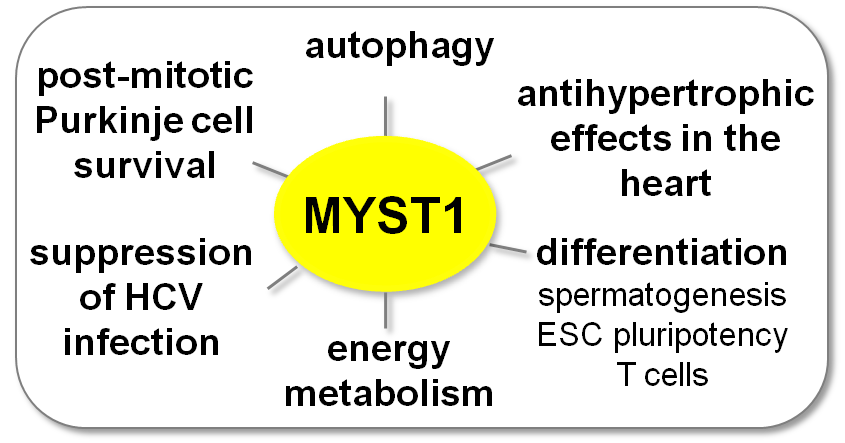
\includegraphics[width=\textwidth]{Figures/MOFothers.png}
 \end{minipage}\hfill
 \begin{minipage}[c]{0.48\textwidth}
	\begin{footnotesize}
   \caption[Functions of the mammalian orthologue of MOF, MYST1.]{\textsf{The mammalian orthologue of \textit{Drosophila} MOF, MYST1, was shown to be required for longevity of Purkinje cells \citep{Kumar2011} and the suppression of hepatitis virus C (HCV) infections \citep{Fusco2013}. It also regulates autophagy \citep{Fullgrabe2013}, protects stressed heart cells from hypertrophy \citep{Qiao2014} and its depletion from the hypothalamus leads to diet-induced obesity \citep{Brenachot2014}. Additionally, its action is needed for the replacement of histones by protamines during spermatogenesis \citep{Meistrich1992,Thomas2007,Lu2010} and MYST1 depletion blocks T cell development \citep{Gupta2013}. Conversely, MYST1 was recently implied in maintaining ESC pluripotency \citep{Li2012}.
}}
\label{fig:MYST}
\end{footnotesize}
 \end{minipage}
\end{figure}
%---------------------------------
%------------------------------
%%% Figure MOF complexes
\begin{figure}
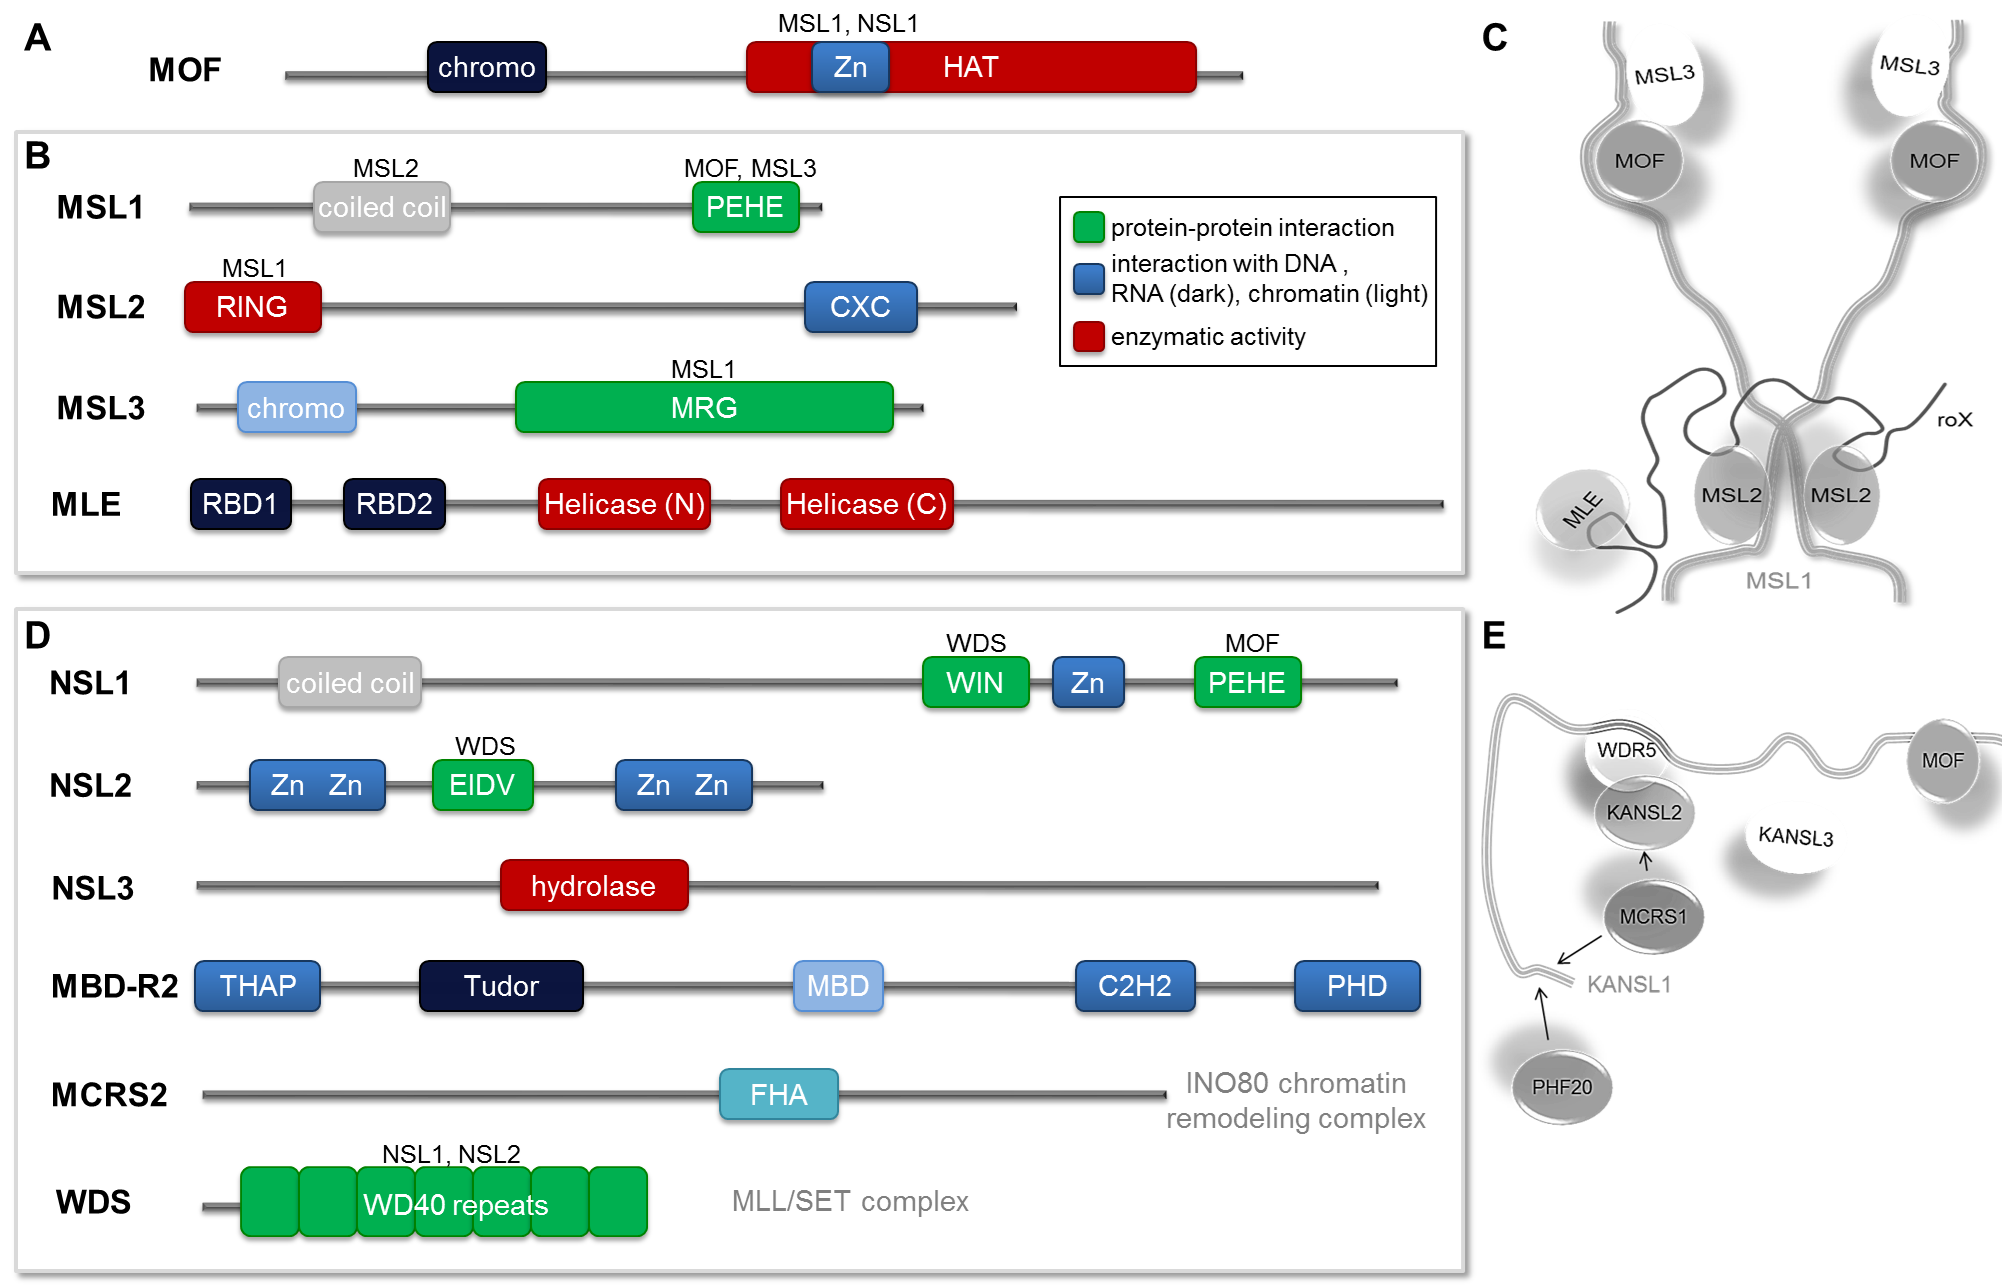
\includegraphics[width=1\textwidth]{Figures/MOFcomplexes.png}
\begin{footnotesize}
\caption[Protein domains and interactions of the MSL and NSL complexes.]{\textsf{Protein domains and interactions of the MSL and NSL complexes.
\textbf{A)} MOF contains a chromo-barrel domain that can bind DNA and RNA and is essential for histone acetylation \citep{Conrad2012}. The zinc finger (Zn) motif within the catalytic HAT domain interacts with MSL1, MSL3 and NSL1 \citep{Morales2004,Kadlec2011}.
\textbf{B)} MSL complex members: The PEHE domain is specific for MSL1-like proteins \citep{Marin2003}. The RING finger domain of MSL2 is required for ubiquitylation and protein-protein interactions \citep{Copps1998,Kruse2009}. MSL3's MRG domain is necessary for the targeting of the male X \citep{Buscaino2003} and preferably binds methylated lysine residues \citep{Moore2010} (\fref{fig:histonesExtended}). MLE contains N-terminal and C-terminal helicase domains with RNA and DNA remodelling activity \citep{Lee1997}.
\textbf{C)} MSL1 is a largely unstructured scaffold protein that dimerizes with MSL2 and subsequently brings together MSL3 and MOF that both interact with MSL1's PEHE domain \citep{Scott2000,Kadlec2011}. \textit{roX} RNA is bound by MSL2 and MLE, completing the complex \citep{Ilik2013}.
\textbf{D)} NSL complex members: NSL1 resembles MSL1, but lacks the region C-terminally of PEHE for the interaction with MSL3 \citep{Smith2005}; instead, like NSL2, it contains an additional WDS-interacting motif (WIN and EIDV, respectively) \citep{Dias2014}. MBD-R2 contains multiple chromatin and nucleic acid interaction motifs; the forkhead-associated domain (FHA) of MCRS2 was shown to bind phosphorylated protein residues and was identified as part of the INO80 complex \citep{}. WDS is a small scaffold protein made up of seven WD40 repeats that is also part of the histone methyl transferase MLL/SET complex \citep{Trievel2009}. 
\textbf{E)} Analogous to the MOF-MSL1 interaction, MOF is recruited into the NSL complex via an interaction with the C-terminal PEHE domain of NSL1 that also interacts with MCRS2, MBD-R2 and WDS \citep{Kadlec2011, Raja2010, Dias2014}. WDS directly interacts with NSL1 and NSL2 \citep{Dias2014}. 
All images are based on figures and data from \citep{Mendjan2006,Kadlec2011,Raja2010,Hallacli2012,Dias2014}.
}}
\label{fig:MOFcomplexes}
\end{footnotesize}
\end{figure}
%----------------------------------------
%
\subsection{The male-specific lethal (MSL) complex and dosage compensation in \textit{Drosophila}}
%
The first known MOF partners were part of the MSL complex which has been well studied in \textit{D. melano\-gaster} where its deletion leads to male-specific lethality.
Like mammals, male and female fruit flies differ in respect to the number of X chromosomes. In contrast to mammals where the inactivation of one of the two female X chromosomes extends the problem of X monosomy to both sexes \citep{Wright2012}, \textit{D.~melano\-gaster} has evolved a chromosome-wide transcriptional upregulation of the single male X chromosome (shown first in 1965 by \citet{Mukherjee1965}) that equalizes the doses of X-linked and autosomal genes in the heterogametic sex. Owing to its male-specific effects on viability and an extraordinary enrichment along the male fly X chromosome, the MSL complex was proposed as they key component of dosage compensation within \textit{Sophophora} species \citep{Ruiz2000} (reviewed by \citet{Laverty2010}).

The exact molecular mechanisms of MSL’s X-specific targeting are not completely elucidated up to date, but many details about the assembly of the complex are now known (see \fref{fig:MOFcomplexes}). The MSL complex is a ribonucleoprotein complex composed of five proteins (MOF, MSL1, MSL2, MSL3 (male-specific lethal 1-3), MLE (maleless)) and one long non-coding RNA (roX1 or roX2 (RNA on X), see \fref{fig:MOFcomplexes} for details and \tref{tab:Names} for synonyms and mammalian protein names). In flies with X:A ratios of one, SXL (sex lethal) inhibits the translation of MSL2 by recruiting the RNA-binding protein UNR (upstream of neuroblastoma rat sarcoma) to the 3’-untranslated region (UTR) of the \textit{msl2} transcript \citep{Abaza2006, Duncan2006, Hennig2014}. Lack of MSL2 suffices to inhibit the formation of the MSL complex in females although all other MSL proteins can in principle be transcribed and translated in both sexes \citep{Gorman1995, Bhadra1999}. While the recognition of the X chromosome is achieved by the MSL1/MSL2 heterodimer \citep{Lyman1997, Kadlec2011}, accumulation along the chromosome and transcription stimulation depend on the presence of \textit{all} MSL proteins (reviewed by \citet{Conrad2011}).

Within the MSL complex, the HAT enzyme MOF has been regarded as the key effector molecule for dosage compensation as the approximately twofold upregulation of X-linked genes in male \textit{Drosophila} seems linked to the long-known hyperacetylation of the male X chromosome \cite{Turner1992,Bone1994}. It was shown that MOF has an extraordinary preference to acetylate lysine 16 of histone H4 (H4K16ac) if accompanied by the MSL complex \citep{Akhtar2000, Smith2000, Li2009, Cai2010} which is in stark contrast to the rather promiscuous acetylation of various histone residues by other known HATs \citep{Lee2007} (\tref{tab:HATs}). The MSL complex, in turn, is responsible for excessive MOF recruitment to the male X chromosome and the subsequent enrichment of H4K16ac along gene bodies \citep{Turner1992, Gelbart2009} that is both stimulated and fine-tuned by the interaction of MOF with MSL complex members \citep{Morales2004, Prestel2010, Kadlec2011}.

Since the MSL complex is absent in female flies, it is unlikely that its presence is required for initial activation of X-linked gene transcription; it is instead thought to recognize already expressed genes that are localized on the X chromosome. The current model delineates that the MSL complex is recruited to several high-affinity binding sites on the X chromosome from where it spreads to active genes (i.a. aided by the binding of MSL3 to methylated H3K36, an abundant mark of on-going transcription \citep{Larschan2007} (\fref{fig:histoneDistribution})) and subsequently enhances the basal transcription rates by acetylation of H4K16 \citep{Conrad2011}. 
%
\subsection{The effects of H4K16ac on chromatin structure}
Acetylation of H3 and H4 tails in general is associated with increased chromatin accessibility as the negative charges of the acetyl group interfere with tight packaging of the poly-anionic DNA strand. In contrast to the acetylation of lysines 5, 8, and 12 of histone H4 that seem to affect the chromatin structure and transcription in a non-specific, cumulative manner, H4K16ac conveys more specific transcriptional effects \citep{Dion2005}. One explanation for H4K16’s special function is its key role in anchoring neighboring nucleosomes where unmodified H4K16 is required for the formation of strong salt bridges between the H4 tail and the acidic patch on the next histone octamer (reviewed by \citet{Kalashnikova2013, Preez2013}). Acetylation of H4K16 disrupts these salt bridges and inhibits chromatin compaction which is in line with the inhibition of chromatin fiber formation that was reported for H4K16ac specifically \citep{Shogren-Knaak2006, Robinson2008}.
%
\subsection{The effects of H4K16ac on transcription}
With the exception of yeast, H4K16ac has unanimously been associated with active transcription as open chromatin in general is a key determinant of gene expression (\citet{Lee2007, Henikoff2011}). In the context of the MSL complex and \textit{Drosophila} dosage compensation, three possible entry points for gene expression enhancement by massive H4K16ac have been proposed: 
\begin{itemize}
\item \textbf{Transcription initiation:} The high accessibility of promoter regions and regulatory elements allows transcription factors to find their cognate target sites more efficiently \citep{Chen2014} and might increase the probability of pre-initiation complex assembly \citep{Conrad2012b}, thereby elevating local concentrations of regulatory proteins and the transcription machinery itself.
\item \textbf{Pol~II pause release:} In mammals, H4K16ac was shown to recruit Brd4 (\fref{fig:histonesExtended}) which in turn recruits P-TEFb, an essential factor for the transition of promoter-bound Pol~II into its actively processing state \citep{Zippo2009} (\fref{fig:Expression}). H4K16ac might thus serve as an additional binding site for transcription-related proteins.
\item \textbf{Elongation of transcription:} Based on the observation that H4K16ac generally covers the entire gene body of dosage-compensated genes with increasing signals towards the 3’-end, it has been suggested that the main effects of H4K16ac for dosage compensation should be on transcription elongation \citep{Smith2001}. This is supported by a recent study reporting Pol~II to reach the 3’-end of genes more easily on the X chromosome compared to autosomes which was dependent on the presence of MSL2 \citep{Larschan2011}. 
\end{itemize}
%---------------------------------------
%%% Figure MOF-complexes-associated functions
\begin{figure}[b!]
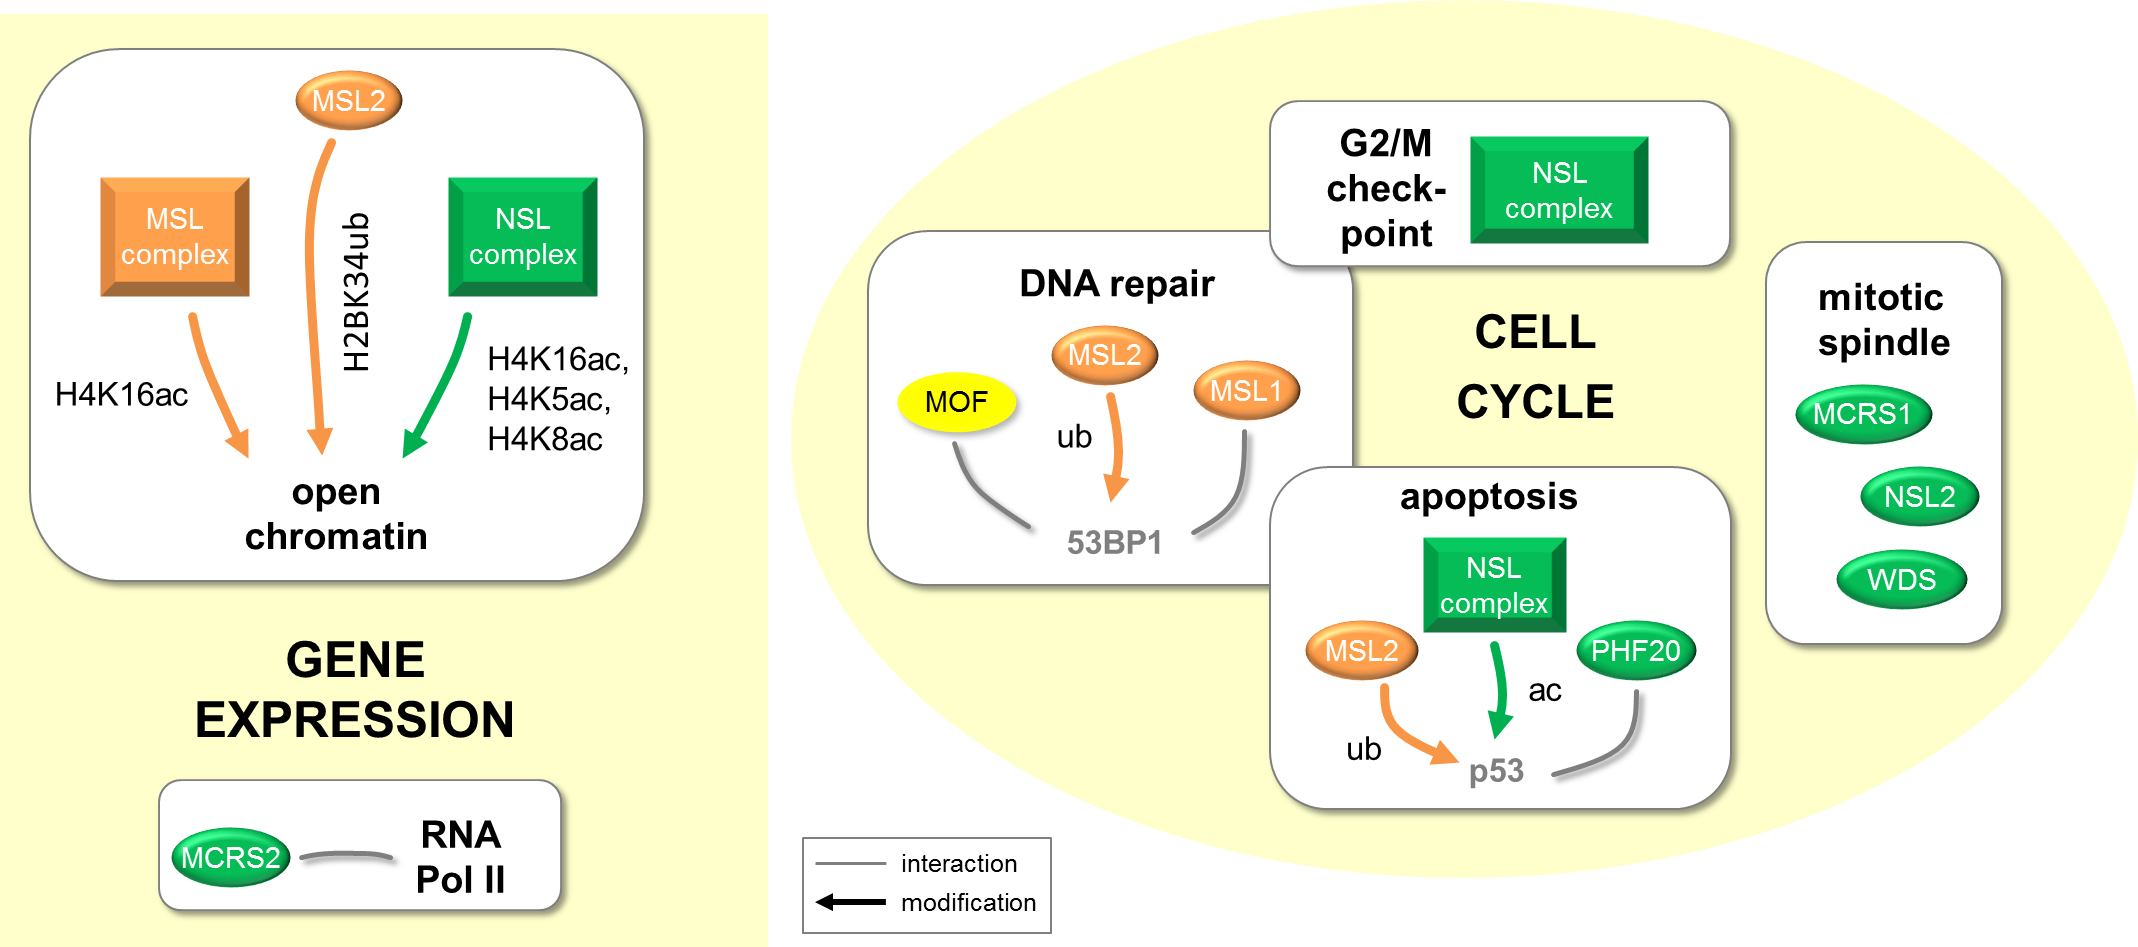
\includegraphics[width=1\textwidth]{Figures/Functions.png}
\begin{footnotesize}
\caption[Molecular functions of MOF and its interaction partners in transcription activation and cell-cycle-related processes.]{\textsf{The vast majority of functions associated with MOF and its interaction partners are related to general transcriptional activation and the cell cycle. Displayed here are those functions that have either been reported to involve MOF within the context of the NSL and MSL complex or individual complex members. Not shown are the roles of WDR5 (WDS) and MCRS1 (MCRS2) as part of the methyl lysine transferase MLL/SET complex and the nucleosome remodelling INO80 complex, respectively.
Grey lines indicate that proteins were found to physically interact, colored arrows indicate post-translational modifications by either MOF (acetylation (ac)) or MSL2 (ubiquitylation (ub)). The details of the function are summarized in \tref{tab:functions1} and \tref{tab:functions2}.
}}
\label{fig:functions}
\end{footnotesize}
\end{figure}
%------------------------------------
The fact that H4K16ac stimulates transcription, perhaps via different mechanisms, is not contested \citep{Birchler2003, Conrad2011}. However, how the approximately twofold upregulation of male single copy X-linked genes to the levels of autosomal genes \citep{Hamada2005, Straub2005} is achieved, has not been solved yet. Given the multiple chromatin, protein, DNA and RNA interaction as well as catalytic domains present in the MSL complex (\fref{fig:MOFcomplexes}, \tref{tab:enzymes}), it is likely that its effects on transcription are manifold and reach beyond H4K16ac to ensure the modest, but vitally important transcription enhancement of male X-linked genes.\\
\begin{minipage}{\textwidth}
\setlength{\abovecaptionskip}{-2ex}
\setlength{\belowcaptionskip}{-2ex}
\vspace*{-2em}
%\begin{landscape}
\begin{minipage}{\textwidth}
\begin{singlespacing}
\begin{small}
\begin{sffamily}
\begin{longtable}[l]{>{\textsf\bgroup}p{3.8cm}<{\egroup} >{\raggedright\arraybackslash}p{2.7cm} >{\textsf\bgroup}p{7cm}<{\egroup}}
\caption[MOF-associated proteins in transcription activation.]{\textsf{MOF-associated proteins in transcription activation. Related to \fref{fig:functions}.}} \\ % the \\ is important! see http://tex.stackexchange.com/questions/103698/extra-alignment-tab-with-longtable
%%%%%%%%%%%%%%%
% table title
\textbf{Proteins} & \textbf{Function} & \textbf{Biological effect}
\tabularnewline \toprule
%\endfirsthead % indicates that the lines above appear as head of the table on the first page
%\multicolumn{3}{c}%
%{\tablename\ \thetable\ -- \textit{Continued from previous page}} \\ [2ex]
%\textbf{Proteins} & \textbf{Function} & \textbf{Biological effect}
%\tabularnewline \toprule \tabularnewline [1ex]
%\endhead % Line(s) to appear at top of every page (except first)
%\multicolumn{3}{r}{\textit{Continued on next page}} \\
%\endfoot % Last line(s) to appear at the bottom of every page (except last)
%\endlastfoot
%%%%%%%%%%%%%%%%%%%
%%% let's start the table content; each column (often) gets its own minipage which enables itemized lists etc.
%%%%%%%%%%%%%%%%%%%
%% first row
%-----------------------
%\\ \multicolumn{3}{c}{\textbf{\textsf{Gene expression}}}
%\\ [2ex] \hline \\ [1ex]
%------------------
\begin{minipage}[c]{3.8cm}
				\vskip 2pt
					MOF within the\\MSL complex \\
				(MSL1, MSL2,\\MSL3, MLE (roX))
				\vskip 2pt
			\end{minipage}
			& \begin{minipage}[c]{2.7cm}
					\raggedright acetylation of H4K16ac \citep{Akhtar2000,Taipale2005,Li2009} \\
			\end{minipage}
					& \begin{minipage}[c]{7cm}
					\vskip 2pt
									\begin{itemize}[noitemsep, leftmargin=*]
										\item opening of chromatin (reviewed by \citet{Preez2013})
										\item dosage compensation in male \textit{D.~melano\-gaster} that entails the upregulation of the entire X chromosome \citep{Conrad2011}
									\end{itemize}				
									\vskip 2pt
							\end{minipage}
%\\ [2ex] \hline \\ [1ex]
\tabularnewline \midrule
%-----------------------
\begin{minipage}[c]{3.8cm}
\vskip 2pt
					MOF within the\\NSL complex \\
				(NSL1, NSL2, NSL3,\\MCRS2, MBD-R2, WDS)
				\vskip 4pt
			\end{minipage}
			& \begin{minipage}[c]{2.7cm}
							\raggedright acetylation of H4K16 \citep{Li2009}, H4K5, H4K8 \citep{Cai2010}
			\end{minipage}
					& \begin{minipage}[c]{7cm} % 3rd column
									\begin{itemize}[noitemsep, leftmargin=*]
										\item opening of chromatin \citep{Preez2013}
										\item housekeeping gene regulation \citep{Feller2012, Lam2012}
									\end{itemize}				
							\end{minipage}
%\\ [2ex] \hline \\ [1ex]
\tabularnewline \midrule
%-----------------------
\begin{minipage}[c]{3.8cm}
					MSL2
			\end{minipage}
			& \begin{minipage}[c]{2.7cm}
			\vskip 2pt
					\raggedright ubiquitylation of H2BK34 \citep{Wu2011}
					\vskip 4pt
			\end{minipage}
					& \begin{minipage}[c]{7cm} % 3rd column
					\vskip 2pt
							implicated to stimulate methylation of H3K4 \citep{Wu2011} and transcription elongation \citep{Wu2014}
							\vskip 4pt
							\end{minipage}
\tabularnewline \midrule
%\\ [2ex] \hline \\ [1ex]
%-----------------------
\begin{minipage}[c]{3.8cm}
\vskip 2pt
					MCRS2
					\vskip 4pt
\end{minipage}
			& \begin{minipage}[c]{2.7cm}
			\vskip 2pt
					interaction partner
					\vskip 4pt
			\end{minipage}
					& \begin{minipage}[c]{7cm} % 3rd column
					\vskip 2pt
							facilitates Pol~II recruitment to target genes \citep{Andersen2010}
							\vskip 4pt
						\end{minipage}
%\\ [2ex] \hline\pagebreak
%-----------------------
%\multicolumn{3}{c}{\textbf{\textsf{Cell-cycle-associated processes}}}
%\\ [2ex] \hline \\ [1ex]
%-----------------------
%%%%%%%%%%%%%%%%%%%%%%%%%%
\tabularnewline \bottomrule
\label{tab:functions1}
\end{longtable}
\end{sffamily}
\end{small}
\end{singlespacing}
\end{minipage}

%\vspace*{-2em}
\begin{minipage}{\textwidth}
\begin{singlespacing}
\begin{small}
\begin{sffamily}
\begin{longtable}[l]{>{\raggedright\arraybackslash}p{3cm} >{\raggedright\arraybackslash}p{11cm}}
\caption[MOF-associated proteins in cell-cycle-related processes.]{\textsf{MOF-associated proteins in cell-cycle-related processes. Related to \fref{fig:functions}}} \\ % the \\ is important! 
%%%%%%%%%%%%%%%
% table title
\textbf{Biological process} & \textbf{Observation} 
\tabularnewline \toprule
%==========================
\begin{minipage}[c]{3cm}
					G2/M checkpoint
			\end{minipage}
					& \begin{minipage}[c]{11cm} % 3rd column
					\vskip 4pt
							NSL1, NSL2, NSL3, MCRS2, MBD-R2 and WDS were identified as essential factors for G2/M checkpoint progression following DNA damage in \textit{D.~melano\-gaster} \citep{Kondo2011}
							\vskip 4pt
							\end{minipage}
\tabularnewline \midrule
%\\ [2ex] \hline \\ [1ex]
%-----------------------
\begin{minipage}[c]{3cm}
					mitotic spindle
			\end{minipage}
					& \begin{minipage}[c]{11cm} % 3rd column
					\vskip 4pt
							\begin{itemize}[noitemsep, leftmargin=*]
							\item NSL2 is needed for mitotic spindle assembly \citep{Goshima2007}
							\item MCRS1 stabilizes the mitotic spindle \citep{Meunier2011}
							\item WDS was identified in a screen for microtubule-associated proteins \cite{Hughes2008}
							\end{itemize}
							\vskip 2pt
							\end{minipage}
\tabularnewline \midrule
%------------------------
\begin{minipage}[c]{3cm}
					apoptosis
			\end{minipage}
					& \begin{minipage}[c]{11cm} % 3rd column
					\vskip 4pt
							\begin{itemize}[noitemsep, leftmargin=*]
							\item ubiquitylation of p53 by MSL2 leads to accumulation of p53 in the cytoplasm \citep{Kruse2009} which is necessary for apoptosis \cite{Muscolini2011}
							\item MOF acetylates p53 in the presence of NSL1 \citep{Li2009} which is necessary for apoptosis induction in cells with DNA damages \citep{Sykes2006, Sykes2009}
							\item human MBD-R2 (PHF20) stimulates expression of p53 and prevents its degradation via a direct interaction with methylated p53 \citep{Park2009, Cui2012}
							\end{itemize}
							\vskip 2pt
							\end{minipage}
\tabularnewline \midrule
%------------------------
\begin{minipage}[c]{3cm}
					DNA repair
			\end{minipage}
					& \begin{minipage}[c]{11cm} % 3rd column
					\vskip 4pt
							\begin{itemize}[noitemsep, leftmargin=*]
								\item MOF is generally required for repair of DNA double strand breaks and recruitment of 53BP1 and BRCA \cite{Sharma2010, Li2010}; its phosphorylated form is particularly important for biasing the cells towards homologous repair during S~phase by displacing 53BP1 from the site of the DNA damage \citep{Gupta2014}
								\item human MSL2 ubiquitylates 53BP1 \citep{Lai2013}
								\item human MSL1 interacts with 53BP1 that positively stimulates DNA damage repair \citep{Gironella2009}
							\end{itemize}
							\vskip 2pt
							\end{minipage}
%%%%%%%%%%%%%%%%%%%%%%%%%%
\tabularnewline \bottomrule
\label{tab:functions2}
\end{longtable}
\end{sffamily}
\end{small}
\end{singlespacing}
\end{minipage}
\end{minipage}
%
\subsection{Individual functions of MSL1 and MSL2}
Evidence for activities of the individual MSL complex members besides MOF predominantly stems from studies on the mammalian orthologues that exist in a sex-independent manner without apparent preference for a particular chromosome (\tref{tab:functions1} and \ref{tab:functions2}). While this seems to strip the MSL complex in mammals of its exceptional and highly visible role for dosage compensation, it also opens up a large scope of putative chromatin-related functions that might not depend on MOF. The ubiquitylation of lysine 34 of histone 2B (H2BK34ub) by MSL2, for example, is stimulated by the presence of MSL1, but not MOF \citep{Wu2011}. Moreover, MSL1 and MSL2 were reported to directly interact with P-TEFb, thereby aiding the transition of Pol~II to elongation \citep{Wu2014} (see \fref{fig:Expression}).

In addition to direct effects on transcription-related processes, MSL1 and MSL2 have been implied in DNA repair and apoptosis, primarily due to their interaction with the tumor suppressor p53 and the p53-binding protein (53BP1) \citep{Kruse2009, Li2010, Lai2013} (see \fref{fig:functions} and \tref{tab:functions2} for details). These tasks do not necessarily exclude the possibility for MOF interactions as histone acetylation and general chromatin relaxation seem to stimulate the DNA repair pathways \citep{Altmeyer2013}, but these findings indicate that, like MOF, MSL proteins might also act outside the MSL complex context, especially in non-sophophora species.
%
\subsection{The non-specific lethal complex and additional MOF targets}
Using mass spectrometry, \citet{Mendjan2006} identified additional, sex-unspecific interaction partners of MOF in fly and human cell cultures which were termed non-specific lethal (NSL) proteins owing to the fact that mutations in their genes killed flies of both sexes.

The NSL complex is comprised of seven proteins: MOF, NSL1, NSL2, NSL3 (non-specific lethal 1-3), MCRS2 (microspherule protein), MBD-R2 (methyl-binding domain protein), and WDS (will die slowly; see \tref{tab:Names} for synonyms and mammalian protein names). At the beginning of my PhD studies, little was known about the cellular task conveyed by the NSL complex, but the first genome-wide study by \citet{Raja2010} had laid the foundation for establishing the NSL complex as a ubiquitous interaction partner that could explain the MSL-independent binding that had been observed for MOF on male as well as female autosomes \citep{Bhadra1999, Kind2008, Raja2010}. Complementary, biochemical experiments revealed that the interaction with NSL proteins relaxes MOF’s substrate specificity towards additional histone residues (H4K5, H4K8) \citep{Cai2010}. Furthermore, MOF was reported to be capable of acetylating non-histone targets which predominantly entail proteins that guard the integrity of the genome, such as ATM (Ataxia Telangiectasia mutated), p53, DBC1 (deleted in breast cancer) and NRF2 (nuclear respiratory factor) \citep{Gupta2005, Sykes2006, Zheng2013, Chen2014}. \citet{Li2009} demonstrated that the interaction with NSL1, but not MSL1, allowed MOF to efficiently acetylate p53 which is important for the induction of apoptosis in cells suffering DNA damage \citep{Sykes2006, Sykes2009}. This finding corroborated the notion that the NSL complex might extend the impact of MOF beyond dosage compensation.
%
\subsection{Individual functions of NSL complex members}
In line with MOF’s acetylation of DNA damage response proteins, it is perhaps more than an interesting side note that all NSL complex members were shown to be essential for the G2/M checkpoint (supplemental material of \citet{Kondo2011}) and individual factors have been described in additional cell-cycle- and DNA-repair-related functions (see \fref{fig:functions}, \tref{tab:functions2}). Besides genome-wide association studies that have implicated mutations in the mammalian orthologues of \textit{Nsl1} and \textit{Nsl2} in different syndromes associated with intellectual disabilities \citep{Itsara2012, Koolen2012, Zollino2012, Gilissen2014}, NSL1-3 have remained largely uncharacterized. The mammalian counterparts of MCRS2 and WDS (MCRS1/MSP58 and WDR5, \tref{tab:Names}) have raised more research interest since they were found within additional multimeric chromatin complexes: MCRS1 was shown to interact with the chromatin remodellers INO80, NuRD and SWI/SNF \citep{Jin2005, Shimono2005, Hsu2012} (\fref{fig:histonesExtended}), while WDR5 is an essential part of the histone methyl transferase MLL \citep{Trievel2009} (mixed-lineage leukemia) that is responsible for trimethylation of H3K4, a prominent histone mark of active gene promoters (\fref{fig:histoneDistribution}). Furthermore, MCRS1 has been identified as an oncogene and a negative regulator of human telomerase reverse transcriptase (hTERT), directly suggesting a substantial influence on cellular senescence signaling \citep{Hsu2012,Hsu2014} (see \tref{tab:cancer} for cancer-related observations for the individual proteins).

As mentioned previously, most studies reporting functions of the (mammalian) NSL complex members examined the proteins in either isolated or different interaction contexts; insights into the functions of the NSL complex as an entity were lacking at the beginning of my PhD studies. One of my major aims therefore was to investigate the chromatin-associated functions of the NSL complex in \textit{Drosophila} and mouse.
%%%%%%%%%%%%%%%%%%%%%%%%%%%%%%%%%%%%%%%%%%%%%%%%%%%%%%%%%%%%%%
\section{ChIP-seq for the study of transcription factor binding}
%
The current state-of-the-art method to examine the binding profiles of DNA- and chro\-ma\-tin-in\-ter\-acting proteins \textit{in vivo} is chromatin immunoprecipitation (ChIP) followed by high-throughput NDA sequencing (seq). The endorsement of ChIP-seq as the major means to study transcription factors and histone modifications in a genome-wide fashion was made possible by the steep decline of costs for DNA sequencing during the past decade which was driven by the development of massively parallel sequencing that, in contrast to the traditional Sanger sequencing, yields rather short (35-100~bp), but highly abundant DNA reads.
%
\subsection{Chromatin immunoprecipitation}
%
%---------------------------------
%%% Figure ChIP-seq bias sources 
\begin{figure}[tb]
 \begin{minipage}[c]{0.65\textwidth}
   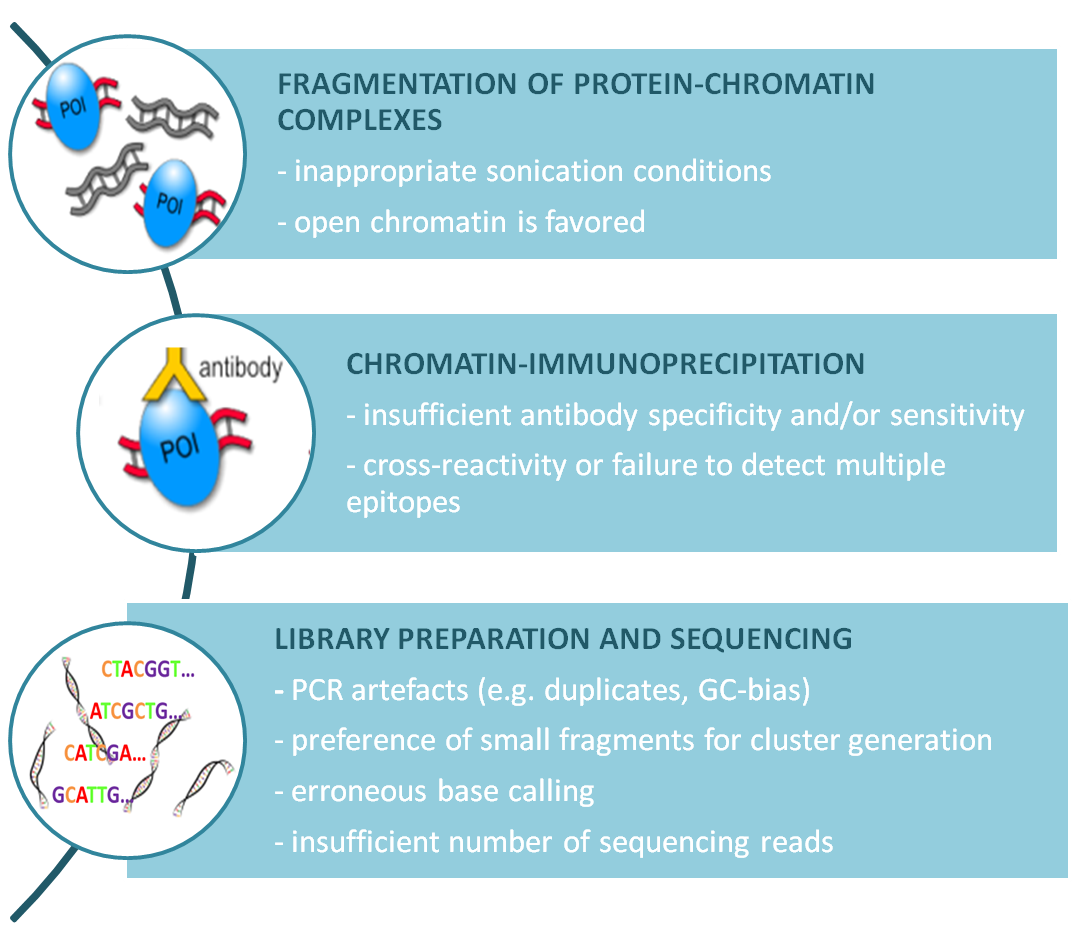
\includegraphics[width=\textwidth]{Figures/chip.png}
 \end{minipage}\hfill
 \begin{minipage}[c]{0.3\textwidth}
	\begin{footnotesize}
   \caption[Technical issues during ChIP-seq experiments that can interfere with the bioinformatic analysis.]{\textsf{Technical issues during ChIP-seq experiments that can interfere with the bioinformatic analysis can occur during every step of the sample preparation. The understanding of the biases introduced by the Illumina sequencing platform has increased profoundly during the past years, but the influence of the fixation and sonication procedures are much less elucidated \citep{Teytelman2013, Gavrilov2014}. See \tref{tab:biases} for details of additional biases. The upper two illustrations were taken from \citep{WikiChIP}.}}
\label{fig:ChIPseq}
\end{footnotesize}
 \end{minipage}
\end{figure}
%---------------------------------
To identify regions of the genome bound by a protein of interest (or marked by a histone modification), the protein-chromatin interactions are usually fixed with formaldehyde before the chromatin is fragmented into pieces of 200-1,000~bp. Then, an antibody against the protein of interest is used to precipitate those fragments to which the protein is bound. After de-crosslinking, the DNA can be purified and sequenced (\tref{tab:sequencing}). Numerous alterations and variations to the basic ChIP protocol exist, such as the use of micrococcal nuclease to fragment the DNA by digestion rather than sonication \citep{Kasinathan2014} and the omission of the formaldehyde fixation (native ChIP) \citep{Neill2003}. The resolution of the binding sites can be increased up to the single base level by applying an exonuclease digestion step after the ChIP (ChIP-exo) \citep{Rhee2011}. Furthermore, Nano-ChIP and linear and \textit{in vitro} transcription (LinDA) have been suggested to enable ChIP-seq with very low cell numbers \citep{Adli2011, Shanka2011}.
%
\subsection{High-throughput sequencing (Illumina platforms)}
Illumina’s high-throughput sequencing method requires short DNA fragments that are eventually hybridized to a sophisticated glass slide, the flow cell (see details in \tref{tab:sequencing}). To ensure a signal that will be unambiguously detected, each fragment is massively and clonally amplified using solid-phase PCR to generate clusters of identical molecules. The sequencing of the fragment ends (35–100~bp) itself is based on fluorophore-labelled dNTPs with reversible terminator elements that will become incorporated and excited by a laser one at a time and thereby enable the identification of single bases \citep{Illumina}. For mammalian genomes, it is recommended to sequence at least 20-60 million DNA fragments, depending on the biological question and the nature of the expected signal \citep{Chen2012, Landt2012, Jung2014}.\\
%%
%
\input{Tables/Table_Sequencing}
%
\subsection{Limitations of ChIP-seq}
Eventhough it is the method of choice for genome-wide transcription factor binding and histone mark profiling, ChIP-seq protocols are prone to biases and artifacts and must therefore be highly optimized (\fref{fig:ChIPseq}, \tref{tab:biases}). There are four factors that determine the success of a ChIP-seq experiment \citep{Liu2010, Chen2012}: the antibody (which must be rigorously tested to exclude cross-reactivity and ensure specificity and sensitivity \citep{Landt2012}), the chromatin extraction (that tends to overrepresent highly transcribed regions \citep{Waldminghaus2010, Teytelman2013}), the library preparation and sequencing (which can introduce several biases) and the bioinformatic analysis that must be tailored to match the data set’s characteristics in order to reveal biologically meaningful insights. It should be noted that all ChIP-seq experiments to date reflect the protein-DNA interactions of a population of cells which suggests that particularly strong signals represent binding sites where the protein of interest is found in the majority of cells.\\
%
\noindent\begin{minipage}{\textwidth} % to avoid pagebreaks despite longtable environment
%\begin{landscape}
\begin{singlespacing}
\begin{small}
\vspace*{-2em}
%\setlength{\abovecaptionskip}{-10pt}
\begin{longtable}{>{\textsf\bgroup\raggedleft\arraybackslash}p{3cm}<{\egroup} >{\textsf\bgroup}p{5cm}<{\egroup} >{\textsf\bgroup}p{6cm}<{\egroup}} % defining the columns - these must match the widths defined for the mini pages down below!
\caption[Biases and artifacts of ChIP-seq data.]{\textsf{Biases and artifacts of ChIP-seq data. Given a rigorously tested antibody, ChIP-seq still suffers from additional technical problems that are due to the sequencing process as well as bioinformatic hurdles.}} \\ % the \\ is important! see http://tex.stackexchange.com/questions/103698/extra-alignment-tab-with-longtable
%%%%%%%%%%%%%%%
% table title
\textbf{Problem} & \textbf{Reasons} & \textbf{Solutions}
\tabularnewline
%-----------------------
\toprule
\begin{minipage}{3cm}
				%\vskip 6pt
					\textbf{Chromatin context} and \textbf{transcription}
				%\vskip 4pt
			\end{minipage}
			&	\begin{minipage}{5cm}
				%\vskip 6pt
				\begin{itemize}[noitemsep,leftmargin=*]
					\item euchromatic chromatin is more easily fragmented
					\item formaldehyde fixation does not capture short-lived protein-DNA interactions \citep{Gavrilov2014} and pref\-er\-en\-tially cross\-links proteins with each other \citep{Neill2003}
					\item chromatin extraction may unspecifically enrich for highly active genes \citep{Teytelman2013}
				
				\end{itemize}
					%\vskip 4pt
			\end{minipage}
			& \begin{minipage}{6cm}
				\vskip 6pt
					\begin{itemize}[noitemsep,leftmargin=*]
						\item cell-type- and condition-specific input controls \citep{Vega2009, Landt2012}
						\item if possible, avoid crosslinking \citep{Neill2003, Kasinathan2014}
						\item optimized chromatin extraction including extensive de-crosslinking, RNase and Proteinase treatments \cite{Waldminghaus2010}
						\item to identify hyper-ChIPable regions, ChIP against a non-endogenous protein was suggested \citep{Teytelman2013}
						\item immunoprecipitation with immunoglobulin G (IgG, mock IP) \citep{Landt2012,Marinov2014}
						
					\end{itemize}	
				\vskip 4pt
			\end{minipage}
\tabularnewline  \hline 
%---------------------------
\begin{minipage}{3cm}
				%\vskip 6pt
					\textbf{Sequencing errors\\and errors in base calling}
				%\vskip 4pt
			\end{minipage}
			& \begin{minipage}{5cm}
				\vskip 6pt
				\begin{itemize}[noitemsep,leftmargin=*]
					\item imperfect sequencing chemistry and signal detection
					\item loss of synchronized base-incorporation into the single molecules within one cluster of clonally amplified DNA frag\-ments (phasing and pre-phasing) (see \tref{tab:sequencing})
					\item signal intensity decay
				\end{itemize}
					\vskip 4pt
			\end{minipage}
				& \begin{minipage}{6cm}
				%\vskip 6pt
					\begin{itemize}[noitemsep,leftmargin=*]
					\item improvement of the sequencing chemistry and detection
					\item optimized software for base calling \citep{Ledergerber2011}
					\item computational removal of bases with low base calling scores \citep{Minoche2011}
					\end{itemize}
				%\vskip 4pt
				\end{minipage}
\tabularnewline  \hline 
%-----------------------
\begin{minipage}{3cm}
				%\vskip 6pt
					\textbf{GC bias} and\\
					\textbf{duplicate reads}
				%\vskip 4pt
			\end{minipage}
			&	\begin{minipage}{5cm}
				%\vskip 6pt
					\begin{itemize}[noitemsep,leftmargin=*]
						\item GC-rich regions are preferably amplified by PCR
						\item small fragments are preferably hybridized to the flow cell
						\item low number of founder DNA frag\-ments
					\end{itemize}
				%\vskip 4pt
			\end{minipage}
			& \begin{minipage}{6cm}
				\vskip 6pt
					\begin{itemize}[noitemsep,leftmargin=*]
						\item optimizing cross-linking, sonication, and the ChIP protocol to ensure that the majority of the genome is present in the sample
						\item limiting PCR cycles during library preparation to a minimum
						\item computational correction for GC content \citep{Cheung2011, Benjamini2012} and elimination of reads from identical DNA fragments
					\end{itemize}	
				\vskip 4pt
			\end{minipage}
\tabularnewline  \hline 
%-----------------------------
\begin{minipage}{3cm}
				%%\vskip 6pt
					\textbf{Copy number\\variations and\\mappability}
				%\vskip 4pt
			\end{minipage}
			&
			\begin{minipage}{5cm}
				%\vskip 6pt
				\begin{itemize}[noitemsep,leftmargin=*]
					\item incomplete genome assemblies
					\item strain-specific differences to the reference assembly may lead to misrepresentation of individual loci
					\item repetitiveness of genomes and shortness of sequencing reads hinder unique read alignment
				\end{itemize}
					%\vskip 4pt
			\end{minipage}
			& \begin{minipage}{6cm}
				\vskip 6pt
					\begin{itemize}[noitemsep,leftmargin=*]
										\item increased sequencing depth and control (non-ChIP) sample aid the computational identification of problematic loci \citep{Bailey2013, Chen2012, Jung2014, Landt2012, Kidder2011}
										\item longer sequencing reads
										\item paired-end sequencing \citep{Chen2012, Bailey2013}
										\item exclusion of blacklisted regions that are known to attract artificially high read numbers \citep{Carroll2014, Blacklists}
										\item computational correction for mappability \citep{Cheung2011}
										\item considering the \textit{effective} genome size \citep{Zhang2008}
					\end{itemize}	
				\vskip 4pt
			\end{minipage}
\tabularnewline \bottomrule
%-----------------------------
\label{tab:biases}
\end{longtable}
\end{small}
\end{singlespacing}
%\end{landscape}
\end{minipage}
%
\subsection{ChIP-seq data processing}
The bioinformatic analysis of ChIP-seq data consists of numerous steps and only the very first tasks are widely standardized: The initial conversion of images of fluorescence into intensity files and ultimately text files that contain the sequencing information is typically done in an automated fashion with vendor-supplied software \citep{Ledergerber2011} (yellow boxes in \fref{fig:ChIPseq}). The resulting file contains all available information for each DNA read, such as the sequence (represented as a string of A, T, G, C), the read ID (referring to the location of the fragment cluster on the flow cell) and quality scores for every base. 
%%%%%%%%%%%%%%%%%%%%%%%%%%
\begin{figure}[tb]
 \begin{minipage}[c]{0.6\textwidth}
   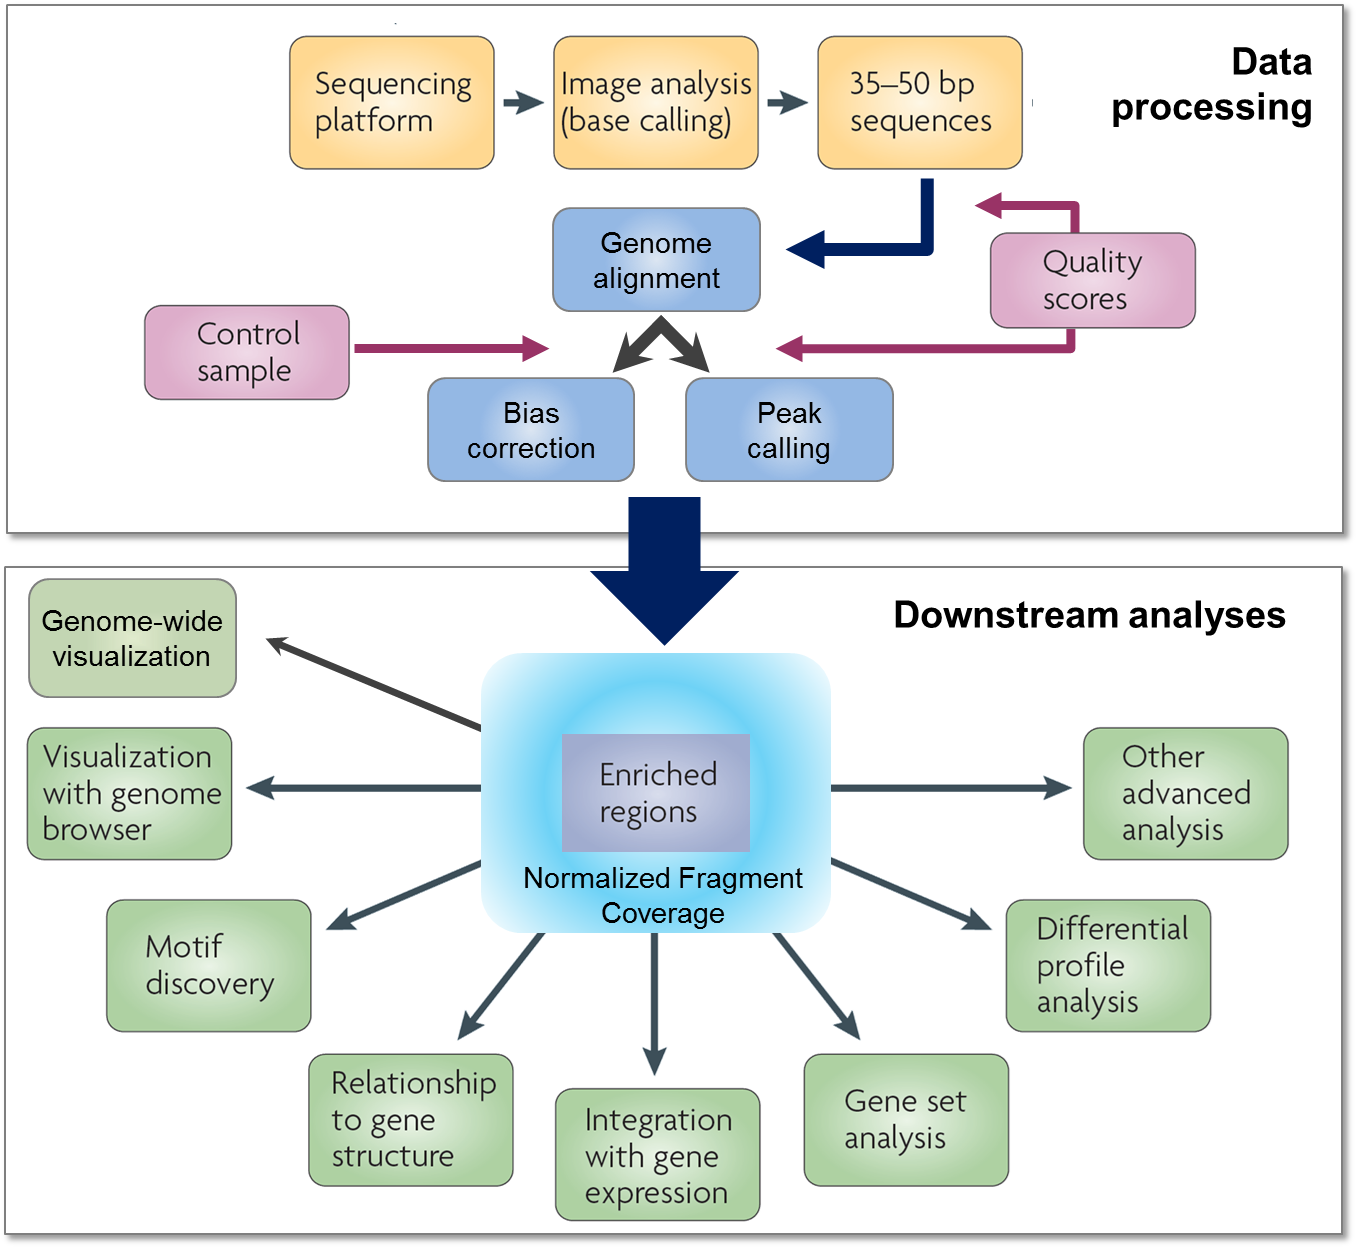
\includegraphics[width=\textwidth]{Figures/DataProcessing.png}
 \end{minipage}\hfill
 \begin{minipage}[c]{0.37\textwidth}
	\begin{footnotesize}
   \caption[Overview of typical computational steps following the completion of high-throughput sequencing.]{\textsf{Overview of typical computational steps following the completion of high-throughput sequencing. The short DNA reads representing the ends of the DNA fragments hybridized onto the sequencer's flow cell are generated by the vendor-supplied software and first need to be aligned to a reference genome. Identification of significantly enriched binding sites (peak calling) and normalized coverage files are the basis for the vast majority of commonly applied ChIP-seq downstream analyses. For more details, see \tref{tab:biases} and the text. I have significantly modified and complemented the original scheme taken from \citet{Park2009}.}}
\label{fig:dataProcessing}
\end{footnotesize}
 \end{minipage}
\end{figure}
%%%%%%%%%%%%%%%%%%%%%%%%%%
Subsequent processing of the sequencing data is aggravated by the large size of the files that require powerful computational infrastructure and efficient handling and manipulation with non-mainstream software tools. UNIX-based operating systems that have traditionally been employed for scientific data analyses provide numerous commands and utilities that tend to perform very specific tasks and are commonly executed through a text-based command interpreter, the UNIX shell. In addition, various programming languages can be used either within the pipelines or for stand-alone scripts (e.g. shell scripts, awk, sed, perl, python, R). Thus, bioinformaticians constantly struggle to find a balance between highly specialized, often improvised solutions and standardized, less flexible programs while trying to ensure reproducibility and transparency through myriad rounds of iteratively adjusted analyses.
%
\subsubsection{Genome alignment}
The first task of any ChIP-seq analysis is to identify the genomic locus of origin for each DNA read. Due to the large number of reads (several millions) and the genome they originated from (almost three giga base pairs for humans), so-called mapping programs must balance accuracy, speed, computational memory usage and flexibility \citep{Leleu2010}. Various mapping algorithms exist \cite{Flicek2009}, the two most commonly used programs are bowtie2 \citep{Langmead2012} and BWA \cite{Li2010a}.

All programs offer manifold options to tune the alignment process to be either faster or more sensitive. Moreover, users can decide how to deal with ambiguous alignments (a read might match more than one region in the genome), gaps and insertions, individual base qualities within a read and mismatches \citep{Langmead2009, Langmead2012}. ChIP-seq data does not strongly depend on the exact DNA sequence of every individual DNA read because the final readout is the number of reads overlapping at particular genomic loci compared to background regions (\fref{fig:readsCoverages}), which is why mapping results are often accepted with 3-5\% of mismatched bases per read \citep{Bardet2012}. Conversely, ChIP-seq samples can suffer severely from biases that affect the distribution of background reads across the genome which must be assessed and ultimately accounted for \citep{Liu2010, Cheung2011, Benjamini2012} (see \tref{tab:biases}). 
%%%%%%%%%%%%%%%%%%%%%%%%%%%%%%%%%%
\begin{figure}[tb]
 \begin{minipage}[c]{0.6\textwidth}
   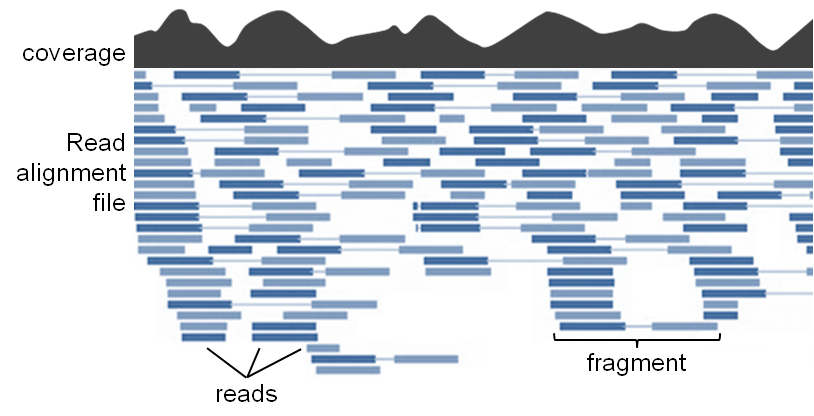
\includegraphics[width=\textwidth]{Figures/CoverageAndReads.png}
 \end{minipage}\hfill
 \begin{minipage}[c]{0.37\textwidth}
	\begin{footnotesize}
   \caption[Snapshot of a typical visualization of DNA read and coverage files.]{\textsf{Snapshot of a typical visualization of DNA read and coverage files. Shown here are paired-end reads, i.e. both ends of each DNA frag\-ment were sequenced (indicated by dark and light blue boxes) and can now be used to easily reconstruct the precise frag\-ments. The coverage shown on top is based on the number of overlapping fragments.}}
\label{fig:readsCoverages}
\end{footnotesize}
 \end{minipage}
\end{figure}
%%%%%%%%%%%%%%%%%%%%%%%%%%%%
\subsubsection{Control sample}
Some biases associated with ChIP-seq data are caused by the genome structure, the chromatin context as well as bioinformatic processing that vitally depends on the state of the genome annotation (\tref{tab:biases}). These systematic errors are generally thought to be controlled by the use of a matching input sample \citep{Kharchenko2008b, Zhang2008, Park2009, Kidder2011, Ho2011, Chen2012, Landt2012}, i.e. a sample that underwent the same treatment as the ChIP-seq sample (in regard to the cell culture, fixation, lysis, fragmentation (\fref{fig:ChIPseq})) with the exception of the immunoprecipitation step. It is recommended to generate a control for every chromatin preparation, for each cell type and condition and to sequence the control at least as deeply as (or preferably deeper than) the ChIP sample \citep{Tuteja2009,Ho2011,Landt2012, Bailey2013}. The goal of the input sample is to have a comprehensive representation of the background reads that should allow the assessment of under- and overrepresented regions due to biological factors (e.g. heterochromatic regions) \citep{Vega2009} as well as technical reasons (e.g. unmappable regions and Ultra High Signal regions \citep{Blacklists}).

To account for biases introduced by the chromatin precipitation (\fref{fig:ChIPseq}, \tref{tab:biases}), some researchers prefer to perform a mock immunoprecipitation (IP) with a non-specific immunoglobulin instead of an input sample \citep{Landt2012}. Unfortunately, the DNA recovery of mock IP experiments can be exceedingly small which could lead to overrepresentation of sequencing artifacts (\tref{tab:biases}). Moreover, it was shown that the use of histone H3 or H4 ChIP-seq does not significantly improve the analysis of ChIP-seq data for histone marks compared to the above mentioned input \citep{Flensburg2014}.
%
\subsubsection{Quality controls and metrics}
%
In the past two years, several measures for the assessment of ChIP-seq data quality have been proposed, most notably by the ENCODE (encyclopedia of DNA elements) consortium that generated hundreds of now publicly available ChIP-seq data sets \citep{Consortium2012}. The quality checks are applied at all stages of the data processing, starting with the determination of contaminant sequences in the raw read files, followed by the quantification of uniquely and non-redundant reads after read alignment and possible overrepresentation of GC-rich regions (\tref{tab:biases}). Reads with more than one optimal alignment locus in the genome are usually filtered out in most ChIP-seq analyses as they might increase the risk of false positive binding site detections. However, if the protein of interest is expected to be enriched at repetitive regions of the genome, it would be detrimental to eliminate these ambiguous reads that usually originate from repeats \citep{Treangen2012}. See \tref{tab:qscores} for the summary of the most widely used quality metrics including those that assess the reproducibility since two replicates per ChIP-seq and input samples are recommended \citep{Rozowsky2009, Landt2012}.

Once the basic sequencing quality properties are checked, scores for signal-to-noise ratios should give an impression of how well the ChIP worked. It is important to note that the vast majority of the quality controls were optimized for ChIP-seq data of transcription factors and histone marks with abundant and very localized enrichments. ChIP-seq experiments with broad, domain-like enrichments or very few binding sites will very often not meet the recommended quality thresholds due to their inherently reduced signal-to-noise ratios \citep{bamFingerprint, Landt2012, Bailey2013, Diaz2012} (\tref{tab:qscores}). 
%
\subsubsection{Normalized fragment coverages}
One part of the ChIP-seq analysis workflow that is often mentioned, but rarely scrutinized in detail is the generation of coverage files for which the read-focused information from the genome alignment is converted into integer counts of the number of reads at a given genomic locus (\fref{fig:dataProcessing}, \fref{fig:readsCoverages}). This conversion serves two purposes: a)~the possibility to adjust for coverage biases and b)~file size reduction which is essential for efficient downstream analysis tools, data sharing and visualization. The aim of the normalization is to make different samples comparable, irrespective of their sequencing depth and additional biases. 

Despite its importance, there is no agreement on the optimal generation of coverage files (except for extending the reads to match the expected original DNA fragment size \citep{Pepke2009, Leleu2010}, \fref{fig:readsCoverages}). Numerous strategies for the normalization of differing numbers of total reads per sample exist (e.g. linear scaling factors calculated with various methods \citep{Kharchenko2008b, Rozowsky2009, Diaz2012}, reads per million per kilobase \citep{Mortazavi2008}, quantile normalization \citep{Mendoza2012}, trimmed mean of M-values \citep{Robinson2010}) and two methods for the correction of GC bias have been presented \citep{Cheung2011, Benjamini2012}.
%
\subsubsection{Identification of binding sites}
In addition to coverage files, downstream analyses of ChIP-seq data are usually based on a set of genome regions that represent loci where the immunoprecipitated protein had bound \citep{Park2009,Liu2010, Bailey2013}. These regions should be overrepresented in the ChIP-seq sample compared to the genome-wide background (hence they are commonly referred to as peaks) and numerous algorithms have been developed to separate binding events from background noise (reviewed by \citet{Pepke2009}). The two basic steps of peak calling are: 1.~identification of regions with large numbers of overlapping reads and 2.~the assessment of the significance of the read enrichment.
The programs choose slightly different approaches for both steps, influencing the sensitivity, specificity, but most strongly the positional accuracy of the peak region predictions \citep{Wilbanks2010}. The reliability of the significance measures absolutely depends on the choice of the statistical model to describe the distribution of background reads which is complicated by the numerous sources of coverage bias mentioned previously and in \tref{tab:biases}. 

One of the most widely used tools, MACS \citep{Zhang2008}, tries to accommodate for the sample-specific influences of the experimental as well as the bioinformatic procedures by utilizing dynamic Poisson distributions. They are parametrized on the background reads of each sample to capture the genome-wide values as well as local biases surrounding any candidate region taking the input control into consideration. To account for false positive calls, MACS version 1.4 calculates an empirical false discovery rate based on significantly enriched regions in the input sample \citep{Zhang2008, Feng2012}. 

Peak calling can be tremendously helpful for ChIP-seq analyses, but thorough benchmarking of the performance of the different algorithms is severely hindered by the lack of a comprehensive list of true binding sites that could be used for a fair comparison. In addition to ChIP-qPCR validation of selected peak regions \citep{Laajala2009}, several proxies for peak quality have been used, such as DNA motif enrichments \citep{Wilbanks2010} and reproducibility between different peak calling algorithms \citep{Laajala2009}. None of these approaches offer a global verification of peak regions, particularly not in regard to their exact position. Therefore, manual inspection is still the method of choice to decide on the success or failure of a peak calling step \citep{Rye2011}. This is especially important when dealing with diffuse, domain-like signals for which great inconsistencies between different peak callers were reported \citep{Ho2011}. 
%
\subsubsection{Downstream analyses}
Exploratory ChIP-seq analyses strongly depend on visualization and unsupervised clustering of the data to unveil unexpected patterns and correlations that can subsequently be experimentally tested \citep{Ramirez2014}. There is virtually no standardization regarding downstream analyses as they must be tailored to the specific biological questions, but the most widely applied strategies are depicted in \fref{fig:dataProcessing}. For example, \textit{de novo} identification of DNA motifs underlying the ChIP-seq peaks is helpful to understand the targeting of a transcription factor \citep{Machanick2011} and gene ontology terms of putative target genes may give clues to the biological role of the investigated protein \citep{Huang2009, Welch2014} (see \tref{tab:tools} for commonly used programs). Furthermore, additional genome-wide data sets are often integrated to complement the ChIP-seq; transcriptomics, for example, can be used to directly correlate the binding of a protein to transcriptional regulation of possible target genes \citep{Chelmicki2014}.
%
\section{Aims}
% Chapter Template

%\chapter{Aims} % Main chapter title

%\label{Aims} % for referencing this chapter elsewhere, use \ref{ChapterX}

%\lhead{Aims} % this is for the header on each page - perhaps a shortened title

%------------------------------------------------------------------
%	SECTION 
The goal of my studies was to gain biological insights from the analyses of the binding profiles of MOF-associated proteins: the non-specific lethal complex (NSL) and the male-specific lethal complex (MSL) members.
The analyses were based on chromatin immunoprecipitation followed by high-throughput sequencing (ChIP-seq). Thus, before the biological questions could be addressed, we first needed to establish robust bioinformatic workflows and scripts ranging from data processing to bias identification and correction and manifold customized downstream analyses. 

In \textit{Drosophila}, we specifically wanted to address whether the different complex members of the NSL complex would co-occur. Moreover, we wanted to infer and subsequently test new hypotheses about the biological function of the NSL complex in regard to gene expression regulation.
Since both MSL and NSL complex had not been previously examined in mammals, we then set out to study their chromatin targeting in mouse cells. To this end, Tomasz Chelmicki generated ChIP-seq profiles of MOF, MSL1, MSL2, NSL3 and MCRS1 in mouse embryonic stem cells and neuronal progenitor cells. The ChIP-seq data study revealed common and different binding principles of the two complexes in pluripotent and differentiated cells which we complemented with transcriptome studies from perturbation experiments and additional genome-wide data sets.





%% Chapter Template

%\chapter{Aims} % Main chapter title

%\label{Aims} % for referencing this chapter elsewhere, use \ref{ChapterX}

%\lhead{Aims} % this is for the header on each page - perhaps a shortened title

%------------------------------------------------------------------
%	SECTION 
The goal of my studies was to gain biological insights from the analyses of the binding profiles of MOF-associated proteins: the non-specific lethal complex (NSL) and the male-specific lethal complex (MSL) members.
The analyses were based on chromatin immunoprecipitation followed by high-throughput sequencing (ChIP-seq). Thus, before the biological questions could be addressed, we first needed to establish robust bioinformatic workflows and scripts ranging from data processing to bias identification and correction and manifold customized downstream analyses. 

In \textit{Drosophila}, we specifically wanted to address whether the different complex members of the NSL complex would co-occur. Moreover, we wanted to infer and subsequently test new hypotheses about the biological function of the NSL complex in regard to gene expression regulation.
Since both MSL and NSL complex had not been previously examined in mammals, we then set out to study their chromatin targeting in mouse cells. To this end, Tomasz Chelmicki generated ChIP-seq profiles of MOF, MSL1, MSL2, NSL3 and MCRS1 in mouse embryonic stem cells and neuronal progenitor cells. The ChIP-seq data study revealed common and different binding principles of the two complexes in pluripotent and differentiated cells which we complemented with transcriptome studies from perturbation experiments and additional genome-wide data sets.




% Chapter Template
\chapter{Results and discussion} % Main chapter title
\label{Results} % for referencing this chapter elsewhere, use \ref{ChapterX}
%\lhead{Results and discussion} % this is for the header on each page - perhaps a shortened title
\fancyhead[RO,LE]{Results and discussion}
\fancyfoot[C]{\thepage}

The following chapter summarizes the methods and insights of the four manuscripts that can be found in the appendix of this thesis.

\aref{SuppPub_NSL} corresponds to Lam, Mühlpfordt, Vaquerizas et al. (2012) \citep{Lam2012} where we examined the \textit{Drosophila} ChIP-seq profiles of four members of the NSL complex (NSL1, NSL3, MCRS2, MBD-R2; generated by Sunil Raja and Kin Chung Lam) and ChIP-seq data for Pol~II from S2 cells depleted of either NSL1 or NSL3 (experiments by Kin Chung Lam).

\aref{SuppPub_MSL} corresponds to Chelmicki, Dündar et al. (2014) \citep{Chelmicki2014} for which Tomasz Chelmicki generated ChIP-seq data of MOF, MSL1, MSL2, NSL3, MCRS1 in mouse embryonic stem cells and neuronal progenitor cells. Matthew Turley and Tasneem Khanam generated transcriptome data for cells depleted of individual factors.

\aref{SuppPub_deepTools} corresponds to Ramirez, Dündar et al. (2014) \citep{Ramirez2014}, the publication of a software suite for quality control, normalization and visualization of high-throughput sequencing data.

\aref{SuppPub_MSL1} corresponds to the submitted manuscript by Chlamydas et al. that focuses on the general role of fly and mammalian MSL1 at promoters and makes use of the ChIP-seq profiles of MSL1 in \textit{D.~virilis}, \textit{D.~melanogaster} and mouse.
%------------------------------------------------------------------
%	SECTION 
%------------------------------------------------------------------
\section{Setting up a ChIP-seq analysis workflow}
One of the main goals of my PhD studies was to identify pitfalls and optimized methods of ChIP-seq analyses whose basics had been established in our group by Sarah Diehl and Thomas Manke. In short, there were three main insights:
\begin{itemize}[topsep=0pt]
\item Understanding biases of the data is crucial for the analysis as well as for improved experimental procedures.
\item Standardized bioinformatic workflows must always be coupled to manual inspections and iterative optimization depending on the quality and nature of the data set and the questions to be answered.
\item Any software for analysis of high-throughput sequencing data must be inherently designed with some flexibility as the applications, sequencing platforms, file formats, data types and statistical models are constantly evolving.
\end{itemize}
%
%--------------------------------------
%%% Figure ChIP-seq workflow
\begin{figure}
 \begin{minipage}[c]{0.6\textwidth}
   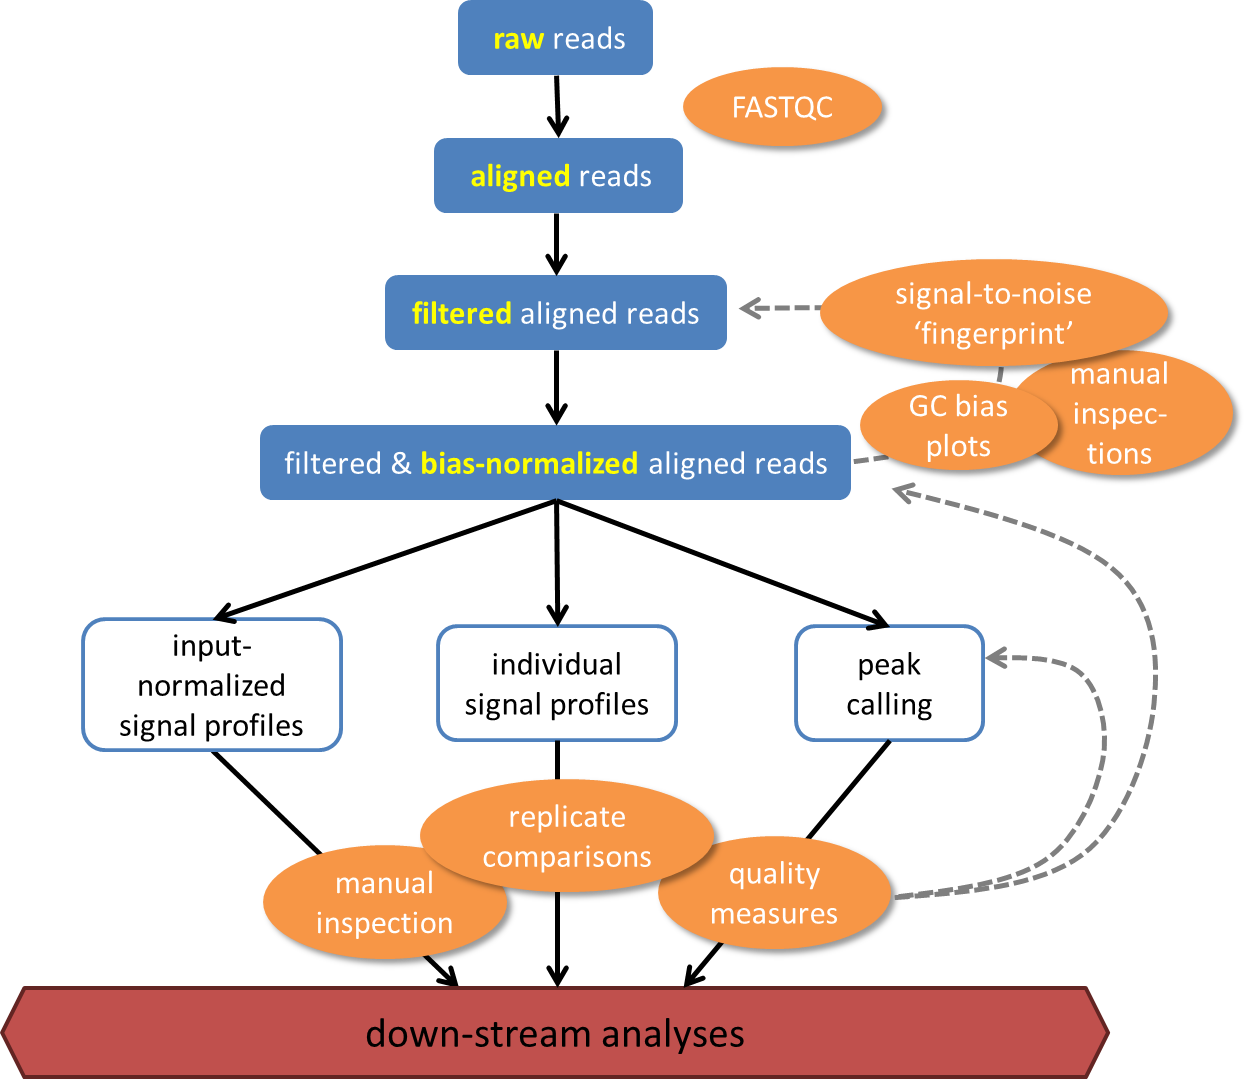
\includegraphics[width=\textwidth]{Figures/workflowChIP-seq.png}
 \end{minipage}\hfill
 \begin{minipage}[c]{0.35\textwidth}
	\begin{footnotesize}
   \caption[General bioinformatics workflow for ChIP-seq analyses.]{\textsf{Schematic of the general bioinformatics workflow for ChIP-seq analyses.
	Orange circles depict quality controls, boxes with solid blue fill indicate read-based files (FASTQ and SAM/BAM, for file name explanations see the glossary of \aref{SuppPub_deepTools}), white boxes indicate files based on genomic intervals. The in\-for\-ma\-tion of the various quality checks help to adjust all steps to match the samples' properties and the ultimate biological questions to be answered.
}}
\label{fig:workflow}
\end{footnotesize}
 \end{minipage}
\end{figure}
%---------------------------------
%
%%\begin{landscape}
\begin{singlespacing}
\begin{small}
%\setlength{\extrarowheight}{15pt} % this doesn't work to control the vertical space
\vspace*{-1em}
\begin{longtable}{>{\textsf\bgroup\raggedleft\arraybackslash}p{2.7cm}<{\egroup} >{\textsf\bgroup}p{4.5cm}<{\egroup} >{\textsf\bgroup}p{4.2cm}<{\egroup}>{\textsf\bgroup}p{2.3cm}<{\egroup}} % defining the columns - these must match the widths defined for the mini pages down below!
\caption[Bioinformatic tools used for analyses presented here.]{\textsf{Bioinformatic tools used for analyses presented here (alphabetical order; if available, I indicated the versions of the tools that I used). For explanations of the file formats mentioned here, please see the glossary within the supplement of \aref{SuppPub_deepTools}.}} \\ % the \\ is important! see http://tex.stackexchange.com/questions/103698/extra-alignment-tab-with-longtable
%%%%%%%%%%%%%%%
% table title
\textbf{Name} & \textbf{Application} & \textbf{Website} & \textbf{Reference}
\tabularnewline \hline
\endfirsthead % indicates that the lines above appear as head of the table on the first page
\multicolumn{4}{c}%
{\tablename\ \thetable\ -- \textit{Continued from previous page}} \\[1ex]
\textbf{Name} & \textbf{Application} & \textbf{Website} & \textbf{Reference}
\tabularnewline \toprule %\tabularnewline [1ex]
\endhead % Line(s) to appear at top of every page (except first)
\multicolumn{4}{r}{\textit{Continued on next page}} \\
\endfoot % Last line(s) to appear at the bottom of every page (except last)
\endlastfoot
%%%%%%%%%%%%%%%%%%%
%% first row
%-----------------------
\toprule %\\ [4ex]
 \begin{minipage}{2.7cm}
				\textbf{bedtools} \\
					(2.10. to 2.17)
				\end{minipage}
			&	 \begin{minipage}{4.5cm}
				working with genomic intervals, e.g. intersecting two files with different peak regions
			\end{minipage} 
			&  \begin{minipage}{4.2cm}
			\url{http://bedtools.readthedocs.org/en/latest/}
			\end{minipage} 
			&  \begin{minipage}{2.3cm}
					\raggedright \citet{Quinlan2010}
				\end{minipage} 
%\\ [4ex] \hline \\ [1ex]
\tabularnewline \midrule
%---------------------------
 \begin{minipage}{2.7cm}
				\textbf{bowtie} \\
					bowtie-1.0.0\\(Appendix \ref{SuppPub_NSL}),\\
					bowtie2-2.2.2\\(Appendix \ref{SuppPub_MSL}) %\\ [2ex]
			\end{minipage} 
			&  \begin{minipage}{4.5cm}
			alignment of reads to the reference genome
				\end{minipage} 
				&  \begin{minipage}{4.2cm}
				\url{http://bowtie-bio.sourceforge.net/index.shtml}
				\end{minipage} 
				&  \begin{minipage}{2.3cm}
				Langmead and\\
				Salzberg \citep{Langmead2012}
			\end{minipage} 
%\\ [4ex] \hline \\ [1ex]
\tabularnewline \midrule
%-----------------------
 \begin{minipage}{2.7cm}
				\textbf{ChIPEnrich}
			\end{minipage} 
			&  \begin{minipage}{4.5cm}
					gene ontology enrichments for target genes identified by ChIP-seq
			\end{minipage} 
			&  \begin{minipage}{4.2cm}
					\url{http://sartorlab.ccmb.med.umich.edu/chip-enrich}
			\end{minipage} 
			&  \begin{minipage}{2.3cm}
				\citet{Welch2014}
			\end{minipage} 
%\\ [4ex] \hline \\ [1ex]
\tabularnewline \midrule
%-----------------------------
 \begin{minipage}{2.7cm}
		\textbf{DAVID}
\end{minipage} 
			&  \begin{minipage}{4.5cm}
				gene identifier mapping and gene ontology term enrichment analyses
			\end{minipage} 
			&  \begin{minipage}{4.2cm}
				\url{http://david.abcc.ncifcrf.gov/}
			\end{minipage} 
				&  \begin{minipage}{2.3cm}
				\citet{Huang2009}
			\end{minipage} 
%\\ [4ex] \hline \\ [1ex]
\tabularnewline \midrule
%-----------------------------
 \begin{minipage}{2.7cm}
					\textbf{deepTools} \\
					(up to 1.5.7) %\\ [2ex]
			\end{minipage} 
			&  \begin{minipage}{4.5cm}
				quality controls of BAM files, normalizations, coverage file generation, visualizations with heatmaps and summary plots %\\ [2ex]
			\end{minipage} 
			&  \begin{minipage}{4.2cm}
				\url{http://deeptools.github.io/} %\\ [2ex]
			\end{minipage} 
				&  \begin{minipage}{2.3cm}
		\raggedright Ramirez, Dündar et al. \citep{Ramirez2014} %\\ [2ex]
			\end{minipage} 
%\\ [4ex] \hline \\ [1ex]
\tabularnewline \midrule
%-----------------------------
 \begin{minipage}{2.7cm}
					\textbf{DESeq}\\
					(1.10.1)
				\end{minipage} 
			&  \begin{minipage}{4.5cm}
				calculating normalized fold change values for Pol~II ChIP-seq data set \citep{EBIroutine}
			\end{minipage} 	
			&  \begin{minipage}{4.2cm}
				\url{http://www-huber.embl.de/users/anders/DESeq/}
			\end{minipage}
				& 
				\begin{minipage}{2.3cm}
		\citet{Anders2010}
			\end{minipage} 
%\\ [4ex] \hline \\ [1ex]
\tabularnewline \midrule
%---------------------------
 \begin{minipage}{2.7cm}
				\textbf{fastqc}
				\end{minipage}
			&  \begin{minipage}{4.5cm}
				quality control of FASTQ files
			\end{minipage} 
			&  \begin{minipage}{4.2cm}
				\url{http://www.bioinformatics.babraham.ac.uk/projects/fastqc/}
			\end{minipage} 
			&  not available
%\\ [4ex] \hline \\ [1ex]
\tabularnewline \midrule
%-----------------------------
 \begin{minipage}{2.7cm}
				\textbf{Galaxy} %%\\ [2ex]
				\end{minipage} 
			&  \begin{minipage}{4.5cm}
				vast collection of tools for manifold tasks including working with genomic intervals, joining of lists, motif search etc. %\\ [2ex]
			\end{minipage} 
			&  \begin{minipage}{4.2cm}
				in-house installation %%\\ [2ex]
			\end{minipage} 
					&  \begin{minipage}{2.3cm}
		\citet{Goecks2010} %%\\ [2ex]
			\end{minipage} 
%\\ [4ex] \hline \\ [1ex]
\tabularnewline \midrule
%-----------------------------
 \begin{minipage}{2.7cm}
					\textbf{ggplot2}\\
					(0.9.3.1)
			\end{minipage} 
			&  \begin{minipage}{4.5cm}
				R package for highly customizable plots (e.g. boxplots, x-y plots, bar charts etc.)
			\end{minipage} 
			&  \begin{minipage}{4.2cm}
				\url{http://ggplot2.org/}
			\end{minipage} 
			&  \begin{minipage}{2.3cm}
		\citet{ggplot2}
			\end{minipage} 
%\\ [4ex] \hline \\ [1ex]
\tabularnewline \midrule
%-----------------------------
 \begin{minipage}{2.7cm}
					\textbf{GREAT}\\
					(2.0)
				\end{minipage} 
			&  \begin{minipage}{4.5cm}
				web-based tool for target gene prediction
			\end{minipage} 
			&  \begin{minipage}{4.2cm}
				\url{http://bejerano.stanford.edu/great/public/html/}
			\end{minipage} 
				&  \begin{minipage}{2.3cm}
		\citet{McLean2010}
			\end{minipage} 
%\\ [4ex] \hline \\ [1ex]
\tabularnewline \midrule
%----------------------------
 \begin{minipage}{2.7cm}
					\textbf{Integrative\\Genomics\\Viewer}\\
					(up to 2.3.32) %\\ [2ex]
			\end{minipage} 
			& 	\begin{minipage}{4.5cm}
				genome browser for visualization of BAM, BED, bigWig and bedGraph files %\\ [2ex]
			\end{minipage} 
			&  \begin{minipage}{4.2cm}
				\url{http://www.broadinstitute.org/igv/} %\\ [2ex]
			\end{minipage} 
				&  \begin{minipage}{2.3cm}
		\citet{Thorvaldsdottir2013} %\\ [2ex]
			\end{minipage} 
%\\ [4ex] \hline \\ [1ex]
\tabularnewline \midrule
%-----------------------------
 \begin{minipage}{2.7cm}
					\textbf{liftover}\\
					(2013)
			\end{minipage} 
			&  \begin{minipage}{4.5cm}
				conversion of sequence coordinates from mm8 assembly to mm9
			\end{minipage} 
			&  \begin{minipage}{4.2cm}
				\url{https://genome.ucsc.edu/cgi-bin/hgLiftOver}
			\end{minipage} 
				&  not available
%\\ [4ex] \hline \\ [1ex]
\tabularnewline \midrule
%-----------------------------
 \begin{minipage}{2.7cm}
				\textbf{MACS}\\
					(1.4.2)
				\end{minipage}
			&	 \begin{minipage}{4.5cm}
				identification of significantly enriched ChIP-seq regions
			\end{minipage} 
			&  \begin{minipage}{4.2cm}
				\url{http://liulab.dfci.harvard.edu/MACS/}
			\end{minipage} 
				&  \begin{minipage}{2.3cm}
		\citet{Zhang2008}
			\end{minipage} 
%\\ [4ex] \hline \\ [1ex]
\tabularnewline \midrule
%-----------------------------
 \begin{minipage}{2.7cm}
				\textbf{MEME}\\
					(4.9.0)
				\end{minipage} 
			&  \begin{minipage}{4.5cm}
				\textit{de novo} DNA motif identification
			\end{minipage}
			&  \begin{minipage}{4.2cm}
				\url{http://meme.nbcr.net/meme/}
			\end{minipage} 
					&  \begin{minipage}{2.3cm}
		\raggedright  \citet{Bailey1994, Machanick2011}
			\end{minipage} 
%\\ [4ex] \hline \\ [1ex]
\tabularnewline \midrule
%-----------------------------
\begin{minipage}{2.7cm}
				\textbf{PeakSplitter}\\
					(1.0)
				\end{minipage} 
			&  \begin{minipage}{4.5cm}
				splitting peak regions predicted by MACS into separate regions based on local minima detection
			\end{minipage} 
			&  \begin{minipage}{4.2cm}
				\url{http://www.ebi.ac.uk/research/bertone/software}
			\end{minipage} 
			&  \begin{minipage}{2.3cm}
		\citet{Salmon2010}
			\end{minipage} 
%\\ [4ex] \hline \\ [1ex]
\tabularnewline \midrule
%-----------------------------
 \begin{minipage}{2.7cm}
					\textbf{samtools}\\
					(0.1.19)
			\end{minipage} 
			&	 \begin{minipage}{4.5cm}
				SAM and BAM file handling (indexing, number of mapped/unmapped and uniquely reads etc.)
			\end{minipage} 
			&  \begin{minipage}{4.2cm}
				\url{http://samtools.sourceforge.net/}
			\end{minipage} 
				&  \begin{minipage}{2.3cm}
		\citet{Li2009}
			\end{minipage} 
%\\ [4ex] \hline \\ [1ex]
\tabularnewline \midrule
%-----------------------------
 \begin{minipage}{2.7cm}
					\textbf{TRAP}\\
					(Annotate v3.04)
				\end{minipage} 
			&  \begin{minipage}{4.5cm}
				transcription factor binding affinity calculation
			\end{minipage} 
			&  \begin{minipage}{4.2cm}
				\url{http://trap.molgen.mpg.de/PASTAA.htm}
			\end{minipage} 
				&  \begin{minipage}{2.3cm}
		\citet{Roider2007}
			\end{minipage} 
%\\ [4ex] \hline \\ [1ex]
\tabularnewline \midrule
%-----------------------------
 \begin{minipage}{2.7cm}
				\textbf{UCSC tools} \\
					(2013)
				\end{minipage} 
			&  \begin{minipage}{4.5cm}
				format conversion (bedGraph to bigWig)
			\end{minipage} 
			&  \begin{minipage}{4.2cm}
				\url{http://www.broadinstitute.org/igv/}
			\end{minipage} 
					&  \begin{minipage}{2.3cm}
		\citet{Kent2010}
			\end{minipage} 
%\\ [4ex] \hline \\ [1ex]
\tabularnewline \midrule
%-----------------------------
 \begin{minipage}{2.7cm}
				\textbf{Venny}\\
					(2007)
				\end{minipage} 
			& 	\begin{minipage}{4.5cm}
				generation of Venn diagrams
			\end{minipage} 
			&  \begin{minipage}{4.2cm}
				\url{http://bioinfogp.cnb.csic.es/tools/venny/}
			\end{minipage} 
			&  not available
%\\ [4ex] \hline \\ [1ex]
\tabularnewline \bottomrule
%-----------------------------
\label{tab:tools}
\end{longtable}
\end{small}
\end{singlespacing}
%\end{landscape}

%
My current workflow for ChIP-seq analysis is depicted in \fref{fig:workflow}. It depends heavily on deepTools, a software package that was developed in collaboration with Fidel Ramírez \citep{Ramirez2014} (\tref{tab:tools}). The workflow begins with the sequencing information stored as DNA reads in FASTQ format (for details on the file formats, see the glossary within the supplement of \aref{SuppPub_deepTools}). The reads are aligned using bowtie2 \citep{Langmead2012} with default parameters. I usually discard unmapped, non-uniquely aligned, duplicated and low-quality reads, as well as those mapped to unassembled and mitochondrial chromosomes, to major satellites and other regions with obvious copy number variations. These rather aggressive filtering steps will probably yield non-optimal results for data sets with expected enrichments along repetitive regions and would have to be adjusted accordingly. However, particularly the removal of regions that consistently accumulated extremely high read numbers in both ChIP and input samples, improved the accuracy of scaling factor calculations and peak calling for the data sets that I analyzed (in line, the ENCODE consortium recently published a list of regions whose exclusion from the analysis improved data processing \citep{Blacklists, Carroll2014}). The optimization of the filtering steps was based on various quality controls, e.g. the assessment of the ChIP strength using the method proposed by \citet{Diaz2012}, manual inspections and GC bias checks.
%
\subsection{GC bias normalization}
%%% Figure GC bias
\begin{figure}[tb]
\centering
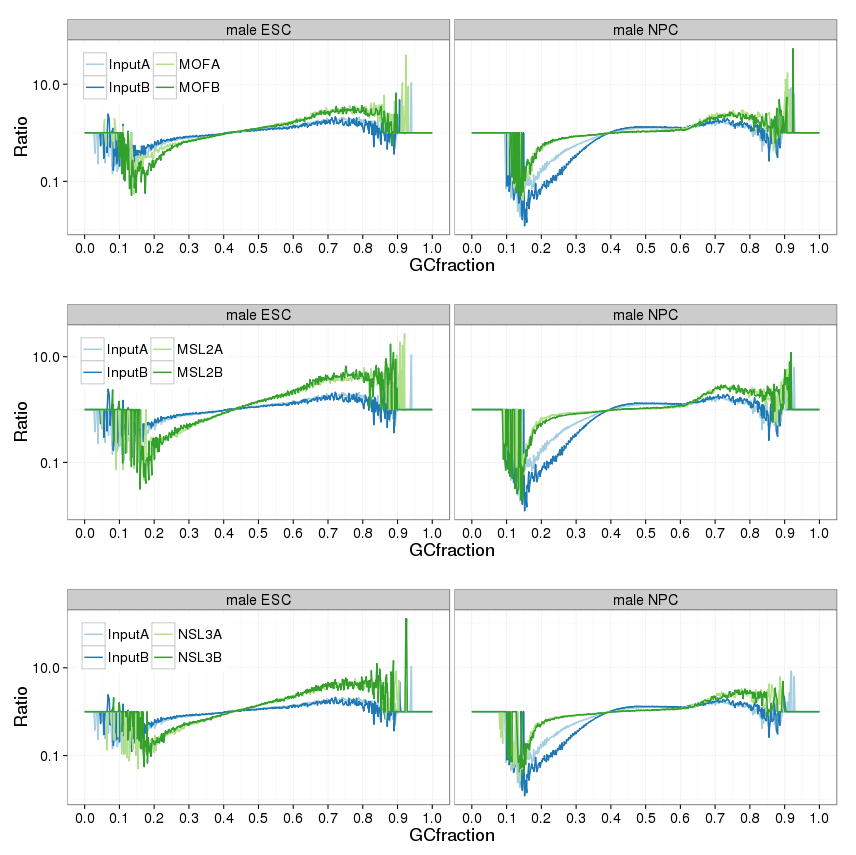
\includegraphics[width=0.9\textwidth]{Figures/ratios_mlES_mlNPC_MOF-NSL3-MSL2.png}
\begin{footnotesize}
\caption[Ratios of observed over expected read counts per GC content bin in ChIP-seq samples from murine embryonic stem cells and neuronal progenitor cells.]{\textsf{Different ratios of observed over expected read counts per GC content bin in ChIP-seq samples from embryonic stem cells (ESC) and neuronal progenitor cells (NPC). Green lines show the ratios for ChIP-seq samples (two replicates each), inputs are shown in blue, note the log scale. Ratios below zero indicate underrepresented regions, ratios above zero overrepresentation. The vast majority of the mouse genome will be covered by regions with 35-60\% GC content, thus any bias between 0.35-0.60 (y-axis) should be paid attention to. The sequencing libraries of the ESC samples were prepared with standard Illumina polymerase, while NPC samples were done with fewer PCR cycles and the HighFidelity Polymerase from New England Biolabs. The lack of AT-rich regions in the input samples is most likely due to other experimental steps than PCR (\tref{tab:biases}). The values underlying the images were calculated with the \texttt{computeGCBias} tool of deepTools \citep{Ramirez2014}.
}}
\label{fig:GCbias}
\end{footnotesize}
\end{figure}
%---------------------------------
The most prevalent and possibly distorting bias that is introduced by Illumina’s PCR-based library preparation and sequencing method (\tref{tab:sequencing}) is the overrepresentation of GC-rich regions. \citet{Benjamini2012} demonstrated that even if the input is handled like the ChIP sample during the experiments, it will unlikely suffice to correct for abundant GC bias because the extent and the regions that are overamplified were shown to be specific for each library preparation. In the light of their insights, we examined the GC bias of the mouse ChIP-seq samples that later on were the basis for Chelmicki, Dündar et al \citep{Chelmicki2014}. As shown in \fref{fig:GCbias}, the different samples indeed had distinct GC bias profiles and the observation that the bias was dramatically reduced when an optimized DNA polymerase and fewer PCR cycles were used (second column of \fref{fig:GCbias}) confirmed the claim of \citet{Benjamini2012} that the DNA amplification steps were the major cause of GC bias. Nevertheless, we identified additional issues that need to be taken into account before adjusting the observed read distributions: 
%
\begin{enumerate}[topsep=0pt]
\item ChIP-seq samples with strong enrichments at mammalian (typically GC-rich) promoters will have a biologically meaningful overrepresentation of GC-regions. This can, for example, be seen in the NPC ChIP-seq samples in \fref{fig:GCbias} where regions with more than 60\% GC content are overrepresented. This is due to the preferred binding of the investigated proteins to CpG-rich promoters.
\item In contrast to the claim that the GC bias should be library-specific, replicates of the same experiment showed very similar GC profiles, indicating a dominant ChIP- (and input-) specific effect.
\item The calculation of the expected read distributions is based on the available genome assembly whose quality might influence the outcome, especially if regions with strong sequence composition biases are not included in the assembly.
\end{enumerate}
%
We addressed the first two issues by a)~excluding unmappable as well as significantly enriched regions from the read distribution calculation and b)~in the case of the non-optimal (standard Illumina) library preparation, we decided to manually scale the input samples to each ChIP-seq so that the input samples reflected the ChIP-seq-specific GC bias rather than eliminating reads from GC-rich regions.

Perhaps the most important insight from these studies was the fact that optimized ChIP and sequencing protocols that were eventually enforced by our in-house sequencing facility almost completely eliminated GC biases. Individual samples at times still indicate the need for computational correction that should, however, be done with care and full knowledge of possible new artifacts that might be introduced such as the loss of enrichments in GC-rich regions\footnote{GC bias correction is applied on the files containing the aligned reads: reads in overrepresented regions are removed randomly, while underrepresented region will obtain artificially duplicated reads.}. In contrast to the BEADS package \citep{Cheung2011} that offers one standardized GC bias correction workflow, deepTools calculates and normalizes the read distributions using two separate tools (\texttt{computeGCbias} and \texttt{correctGCbias}, \aref{SuppPub_deepTools}), so that users can explore the expected and observed values first and thereupon decide which normalization strategy might best suit their data set. 
%
\subsubsection{Normalization for sequencing depth and input control}
Once the read alignments have been thoroughly checked and possibly normalized, the next steps lay the foundation for the majority of ChIP-seq downstream analyses that are typically not dependent on the DNA sequence of each read, but instead rely on summaries of the number of overlapping reads at each given locus in the genome (\fref{fig:readsCoverages} and white boxes in \fref{fig:workflow}).
I will usually first generate coverage profiles for each sample individually, normalizing for sequencing depth only:
\begin{center}
$normalized\:bin\:coverage = \frac{observed\:bin\:coverage \times e\!f\!\!f\!ective\:genome\:size}{mapped\:reads \times f\!ragment\:length}$\\
\end{center}
These profiles are useful to confirm that the input-normalized ChIP-seq signals and the peak calling results (see below) match the patterns seen in the simple coverages.

For input normalization, both input and ChIP must be made comparable first before calculating the ChIP enrichments ($log_2\frac{ChIP}{input}$) for each consecutive genomic bin. If the output of deepTools’ \texttt{bamFingerprint} \citep{Diaz2012} indicates a clear ChIP-seq signal compared to the input \citep{bamFingerprint}, I tend to use the signal extraction scaling (SES) proposed by \citet{Diaz2012}. SES is based on the assumption that the ChIP-seq sample contains both background and immunoprecipitated DNA and that the scaling factor for sequencing depth adjustment should be based on the background signal only. In a plot depicting the cumulative percentage of reads, the input should show a linear increase as each genome region should contain a similar fraction of reads (see the image of \texttt{bamFingerprint} in the supplemental material of \aref{SuppPub_deepTools}). ChIP-seq data, however, will contain a significant fraction of regions with consistently very few reads (= background) and a relatively small number of regions with exceedingly large read numbers (= immunoprecipitated DNA). The SES factor is the ratio of ChIP-seq over input reads at the point where the percentage of input reads maximally exceeds the percentage of ChIP-seq reads \citep{Diaz2012}.
If the separation between background and enrichment signal is not possible, the total number of reads of the less deeply sequenced sample ($n$) can be used to adjust the sequencing depths:
\begin{center}
$ scale\:f\!actor = \frac{n}{mapped\:reads}$ \\
\end{center}
All above described methods are implemented in \texttt{bamCoverage} and \texttt{bamCompare} of the deepTools suite (\aref{SuppPub_deepTools}).
%
\subsection{Peak calling}
%
As described in the introduction, the identification of significantly enriched genome regions is central to the majority of ChIP-seq analysis \citep{Bailey2013} (\fref{fig:dataProcessing}). I chose different peak calling strategies to meet the distinct challenges of each analyzed data set (summarized in \tref{tab:peakCallingStrategies}). All approaches rely on stringent filtering after obtaining the initial lists of significantly enriched regions, but only the Pol~II ChIP-seq and the mouse data set allowed for additional selection of peaks found in two replicates. 
%
%\begin{landscape}
\begin{singlespacing}
\begin{small}
\begin{longtable}{>{\textsf\bgroup}p{3.5cm}<{\egroup} >{\textsf\bgroup}p{4cm}<{\egroup} >{\textsf\bgroup}p{8cm}<{\egroup}>{\textsf\bgroup}p{6.5cm}<{\egroup}} % defining the columns - these must match the widths defined for the mini pages down below!
\caption[Peak calling strategies adjusted for the different sample characteristics.]{\textsf{Peak calling strategies adjusted for the different ChIP-seq sample characteristics.}} \\ % the \\ is important! 
%%%%%%%%%%%%%%%
% table title
\textbf{ChIP-seq sample} & \textbf{Issues} & \textbf{Strategy} &  % 
\tabularnewline \hline
\endfirsthead % indicates that the lines above appear as head of the table on the first page
\multicolumn{4}{c} 
{\tablename\ \thetable\ -- \textit{Continued from previous page}} \\
\textbf{ChIP-seq samples} & \textbf{Issues} & \textbf{Strategy} &  % 
\tabularnewline \toprule \tabularnewline [1ex]
\endhead % Line(s) to appear at top of every page (except first)
\hline \multicolumn{4}{r}{\textit{Continued on next page}} \\ %
\endfoot % Last line(s) to appear at the bottom of every page (except last)
\endlastfoot
%%%%%%%%%%%%%%%%%%%
%%% let's start the table content; each column (often) gets its own minipage which enables itemized lists etc.
%%%%%%%%%%%%%%%%%%%
%% first row
%-----------------------
\toprule
\begin{minipage}[c]{3.5cm}
NSL1, NSL3,\\MCRS2, MBD-R2 in\\\textit{D.~melanogaster}
\end{minipage}
			& \begin{minipage}[c]{4cm}
			peak regions often contained more than one local maximum due to the gene-dense nature of the \textit{Drosophila} genome
			\end{minipage}
				& \begin{minipage}[c]{8cm}
				\begin{enumerate}[noitemsep, leftmargin=*]
					\item peak calling with MACS 1.4.2 with default parameters \citep{Feng2012}
					\item peaks with FDR $\leq$ 5\%
					\item identification of smaller \textsl{subpeaks} with PeakSplitter \citep{Salmon2010}
				\end{enumerate}
				\end{minipage}
					& \begin{minipage}[c]{6.5cm}
					\parbox[c]{1em}{
						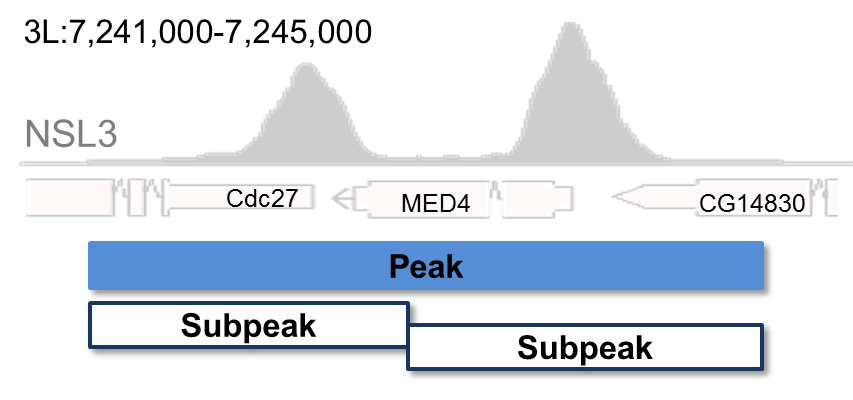
\includegraphics[width=6.5cm,trim=2 2 2 2,clip]{Figures/PeakCalling_Dmel}}
				\end{minipage} 
%\\ [2ex]  \hline \\ [1ex]
\tabularnewline \midrule
%-----------------------
\begin{minipage}[c]{3.5cm}
Pol~II in\\\textit{D.~melanogaster} cells\\(depleted of NSL1 or NSL3)
\end{minipage}
	& \begin{minipage}[c]{4cm}
	the mixed signal of Pol~II (localized, TF-like enrichments around TSS, broad, shallow enrichments along gene bodies) was not well captured by MACS
		\end{minipage}
		& \begin{minipage}[c]{8cm}
\vskip 6pt
				\begin{enumerate}[noitemsep, leftmargin=*]
					\item a symmetric null distribution was fitted to regions with negative enrichments, i.e. where the input signal exceeded the ChIP signal \citep{EBIroutine} (black line)
					\item genomic bins that deviated from the expectation (compare the blue with the black line) were determined as significantly enriched (threshold: q-value $\leq$ 0.05) \\ [2ex]
				\end{enumerate}
\vskip 4pt
			\end{minipage}
				& \begin{minipage}[c]{6.5cm}
						\parbox[c]{1em}{
						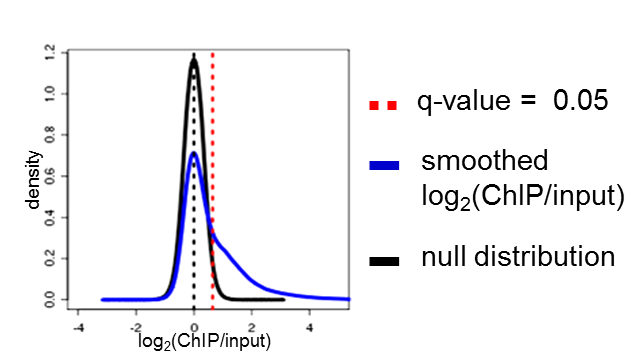
\includegraphics[width=6.5cm,trim=4 4 4 4,clip]{Figures/PeakCalling_PolII}}
					\end{minipage}
%\\ [2ex] \hline \\ [1ex]
\tabularnewline \midrule
%-----------------------
\begin{minipage}[c]{3.5cm}
MOF, MSL1, MSL2,\\NSL3, MCRS1 in\\ mouse ESCs and NPCs
\end{minipage}
	& \begin{minipage}[c]{4cm}
	non-optimal signal-noise ratios, GC bias
		\end{minipage}
		& \begin{minipage}[c]{8cm}
\vskip 6pt
				\begin{enumerate}[noitemsep, leftmargin=*]
                    \item in ESCs: adjustment of the GC bias in the input sample to match each ChIP-seq sample's GC bias
					\item peak calling with MACS 1.4.2 with default parameters \citep{Feng2012} for each ChIP-seq replicate (blue boxes) and the merged file (red box)
					\item only peaks that were present in both replicates and met the FDR threshold of $\leq$ 1\% were used \\ [2ex]
				\end{enumerate}
\vskip 4pt
			\end{minipage}
				& \begin{minipage}[c]{6.5cm}
\vskip 6pt
						\parbox[c]{1em}{
						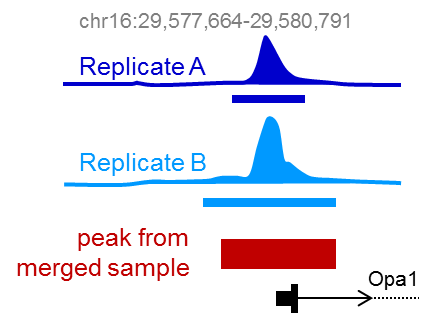
\includegraphics[width=5.5cm,trim=4 4 4 4,clip]{Figures/PeakCalling_Mm}} 
\vskip 4pt
					\end{minipage}
%\\ [2ex] \hline \\ [1ex]
%-----------------------
\tabularnewline \bottomrule
\label{tab:peakCallingStrategies}
\end{longtable}
\end{small}
\end{singlespacing}
\end{landscape}
 % moved to appendix
%
\subsection{Exemplary downstream analyses}
%---------------------------------
%%% Figure Summary plots and heatmaps of NSL, MSL in D.mel 
\begin{figure}[tb]
\centering
\includegraphics[width=.77\textwidth]{Figures/geneProfiles.pdf}
\begin{footnotesize}
\caption[ChIP-seq signals of MSL and NSL complex members in \textit{Drosophila}.]{\textsf{Summary plots and heatmaps of various ChIP-seq signal and GC content for \textit{Drosophila} genes on the X chromosome (chrX) and chromosome 2L (chr2L).
\textbf{A)} MSL complex members in female flies do not distinguish between X and autosomal genes.
\textbf{B)} MSL complex members in male flies show drastically enriched signals along the majority of X-chromosomal genes (lower panel).
\textbf{C)} Visualization of the GC content along fly genes that reveals the difference of GC content between the autosomal chromosome 2Land the X chromosome.
\textbf{D)} NSL complex members in male salivary glands and S2 cells do not distinguish between genes on the X and the autosomal chromosome. All images were generated with \texttt{computeMatrix} and \texttt{heatmapper} from the deepTools suite (\aref{SuppPub_deepTools}) using the scale-regions mode to scale gene bodies to 2~kb. See \tref{tab:ChIPseqSamplesDmel} and \ref{tab:Becker} for details about the ChIP-seq data sets.
}}
\label{fig:profiles}
\end{footnotesize}
\end{figure}
%
The analyses presented in \aref{SuppPub_NSL} and \aref{SuppPub_MSL} were driven by two different basic questions: in Lam, Dündar, Vaquerizas et al. \citep{Lam2012} we focused on the \textit{similarities} of the binding patterns of the NSL complex members in \textit{D.~melano\-gaster} while our study of both MSL and NSL proteins in mouse cells \citep{Chelmicki2014} aimed at identifying the possibly distinct functions of the complexes. I would like to point out three of the most important analysis strategies that formed the basis for almost all subsequent investigations. The details of all downstream analyses, including those related to DNA motif analysis and the integration of numerous published data sets can be found in the methods parts of \aref{SuppPub_NSL} and \ref{SuppPub_MSL}. Furthermore, \tref{tab:tools} gives an overview of the software tools I used.
%
\subsubsection{Binding profiles of MSL and NSL proteins}
Both studies were based on the insights from so-called metagene analyses (or more generally: summary plots) and heatmaps. Summary plots depict the average ChIP-seq signal over an arbitrary number of genome regions (see Box 3 in \citep{Ferrari2014}) while heatmaps allow more detailed views of virtually any kind of genome-wide data. Both types of images can be efficiently produced with \texttt{profiler} and \texttt{heatmapper} of the deepTools suite \citep{Ramirez2014} (see Figures 3E, 4A and Figure supplement 3 of \aref{SuppPub_MSL} for examples).

The summary plots and heatmaps in \fref{fig:profiles} demonstrate that the ChIP-seq enrichments of the individual MSL complex members differ significantly between autosomal and X-linked genes in males as it had been reported before \citep{Alekseyenko2006, Kind2008, Straub2013}. We found that the signals of the NSL complex members, however, are not strongly influenced by the chromosome.

In mice where both complexes are expressed and presumably assembled in a sex-in\-de\-pen\-dent manner we did not detect the broad enrichments typical of dosage-compensated fly genes, but instead narrow, localized signals, preferably around the TSS of active genes (MOF, NSL3, MCRS1) or at putative regulatory sequences (MSL1, MSL2; see \aref{SuppPub_MSL}). 
\clearpage
%
\subsubsection{Identifying target genes}
In addition to describing the binding patterns of the proteins of interest, the characterization of the target genes is of eminent importance for gaining biological insights. The identification of target genes is usually done on the basis of proximity (e.g. peaks close to the promoter of a gene), but it can be significantly enhanced by taking additional criteria into consideration such as the number and intensity of peaks, expression data from perturbation experiments and binding site conservations \citep{Sikora2013}. In Lam, Mühlpfordt, Vaquerizas et al. \cite{Lam2012}, we used very narrow regions to account for the gene-dense nature of the fly genome: Genes were classified as NSL targets if the summit regions of peaks of \textit{all} four profiled proteins (NSL1, NSL3, MCRS2, MBD-R2) overlapped within 200~bp up- or downstream of the transcription start site (TSS). For the mammalian proteins, we identified an initial set of targets if a peak overlapped within 1~kb upstream of a gene’s TSS. We then refined these targets by requiring multiple overlapping peaks as well as significantly affected expression after shRNA-mediated depletion of the respective proteins (\aref{SuppPub_MSL}).

Identifying target genes that may be regulated via promoter-distal binding in introns or intergenic regions is less straight-forward as no clear rules for enhancer-gene associations have been established although proximity seems to perform reasonably well \citep{Shen2012}. Since a profound number of MSL1, MSL2 and NSL3 binding sites in the mammalian cells were located promoter-distally, I made use of GREAT, a web-based program that predicts putative target genes of \textit{cis}-regulatory regions \citep{McLean2010} (see \tref{tab:tools}).
%
\subsubsection{Unsupervised clustering of ChIP-seq signals}
While the ChIP-seq studies of the MSL complex (but not the NSL complex) in \textit{D.~melano\-gaster} had been supported by a substantial body of literature on the biological role of the complex \citep{Taipale2005}, very little was known about the functions of the mammalian orthologues of MSL and NSL complexes. Structural and biochemical studies eventually demonstrated that the mammalian proteins, too, were able to form two distinct MOF-containing complexes \citep{Kadlec2011,Hallacli2012,Dias2014,Ravens2014}, but whether the proteins would predominantly bind the same target genes or rather carry out independent functions remained elusive. In addition, we wanted to examine whether the binding patterns were changing in murine embryonic stem cells (ESC) compared to neuronal progenitor cells (NPC). To obtain a comprehensive impression of all the enrichments in both cell types, hierarchical clustering proved to be a powerful method to reveal the underlying patterns of exclusive and co-occurring enrichments in an unbiased manner. The method described in \aref{SuppPub_MSL} yielded a robust and insightful result\footnote{In brief, I worked on the union of all peaks from both cell types which were scaled to 1.2~kb; normalized signal values were calculated for 50~bp bins for each ChIP-seq sample. The resulting matrix was rank-transformed, converted into Euclidean distance measures and clustered with the hclust function of R (ward linkage) \citep{R}. The rank transformation proved to be the most important step while changing the distance and linkage methods had little effects on the outcome.} that is shown in Figure 2 of \aref{SuppPub_MSL}.
%
The main findings were: 
\begin{itemize}[topsep=0pt]
\item MOF predominantly associates with the NSL complex at gene promoters.
\item There is a small subset of (mostly non-promoter) regions where MOF associates almost exclusively with the MSL complex.
\item Particularly MSL2 binds to a significant number of intergenic and intronic binding sites where none of the other proteins investigated in our study were found.
\end{itemize}
%
%%%%%%%%%%%%%%%%%%%%%%%%%%%%%%%%%%%%%%%%%%%%%%
\section{The roles of MOF within its distinct complexes}
%%%%%%%%%%%%%%%%%%%%%%%%%%%%%%%%%%%%%%%%%%%%%%
\subsection{MOF within the MSL complex}
In \textit{Drosophila}, the function of MOF within the male-specific complex seems well established: it catalyzes the massive acetylation of H4K16 at the male X chromosome, thereby enhancing its transcription. In mammals, the MSL complex has retained its ability to enhance H4K16ac by MOF but besides the general opening of chromatin and transcription enhancement (from promoters as well as enhancers \citep{Taylor2013}), no specific cellular mechanism that solely depends on H4K16ac could be pin-pointed yet. Of note, the decisive role of MSL1 and MSL2 for the maintenance of X chromosome expression in mouse ESCs (see below) does not depend on MOF.
%
\subsection{MOF within the NSL complex}
An initially surprising finding from the mammalian study of NSL and MSL complexes was that MOF seemed to almost always be accompanied by a member of the NSL complex which would only sometimes be complemented by signals from the MSL complex. (Interestingly, \fref{fig:NSLtargetgenes} reveals that in flies, too, MSL and NSL complexes have largely overlapping target gene sets as all NSL-bound genes contain strong signals of the MSL complex.) The transcriptomes of shRNA-treated cells confirmed the notion that the NSL complex might be the predominant interaction partner in mammalian cells: the effects on gene expression were very similar in MOF- and NSL3-depleted cells, but differed significantly from MSL1 or MSL2 depletions (see Figure 3E-G of \aref{SuppPub_MSL}). A remarkable example was the negative effect of MOF and NSL3 depletion on the expression of key pluripotency factors and subsequent loss of pluripotency which was not observed in MSL1- or MSL2-depleted ESCs (\aref{SuppPub_MSL}).

Conversely, in flies MOF’s presence at NSL-bound promoters does not closely mirror the broader gene enrichments of H4K16ac (\fref{fig:profiles}). This could well be due to technical artifacts as the formaldehyde fixation might not capture a transient and less abundant binding of MOF along gene bodies in contrast to the more stable histone modification \citep{Gavrilov2014} (\tref{tab:biases}). However, several HAT complexes contain bromodomains which could bind H4K16ac at the promoter and perhaps mediate spreading of the signal \citep{Forsberg2001} (\fref{fig:histonesExtended}). p300/CBP, for example, was recently shown to be capable of binding to and catalyzing H4K16ac \textit{in vitro} \citep{Filippakopoulos2012, Henry2013}. The histone acetyl transferase ATAC2 (a GNAT family HAT, \tref{tab:HATs}) also contributes to bulk H4K16ac levels in fly embryos and mice \citep{Suganuma2008, Guelman2009}, and interestingly, it strongly interacts with WDS (WDR5 in mammals). Since WDS is part of the NSL complex, one could speculate about ATAC2 recruitment to promoters of NSL targets and subsequent spreading of H4K16ac. It should be noted though that the previously proposed concomitant interaction of WDR5 with both MLL and NSL complexes \citep{Dou2005} was recently shown to be of mutually exclusive nature \citep{Dias2014}, indicating that WDR5 might not be able to act as a bridging factor between different complexes.

Surprisingly, the results of our studies suggest that H4K16ac may not be the major mechanism through which the NSL complex conveys its essential functions (although the NSL1-MOF interaction is very similar to the MSL1-MOF interaction and both increase MOF’s HAT activity \citep{Li2009, Kadlec2011}). The ablation of individual NSL complex members in both \textit{Drosophila} and mammalian cells affects H4K16ac levels only moderately (MCRS2 \citep{Raja2010}) or not at all \citep{Ravens2014} (NSL1, NSL3, MBD-R2; see \aref{SuppPub_NSL} and \ref{SuppPub_MSL}).
In flies, MSL1 might maintain H4K16ac levels in the absence of NSL proteins since it binds to the same promoters (\fref{fig:NSLtargetgenes}). Regardless of the NSLs' influence on H4K16ac, however, H4K16ac does not seem to be the most vital function as female flies can survive until adulthood without MOF, although with compromised longevity and fertility \citep{Hilfiker1997,Conrad2012}. 
In mice, on the other hand, lack of MOF is lethal which indicates that it must play an essential role. The recently discovered ability of MOF to acetylate non-histone proteins may link MOF more directly to vital cellular processes, possibly even in the context of the NSL complex. The regulation of p53-dependent apoptosis induction following DNA damage, for example, relies on the acetylation of p53 by MOF \citep{Sykes2006,Sykes2009} and was shown to be enhanced by NSL1, but not MSL1 \cite{Li2009}.
%%%%%%%%%%%%%%%%%%%%%%%%%%%%%%%%%%%%%%%%%%%%%%
\section{The NSL complex regulates housekeeping genes in\\\textit{D.~melano\-gaster} and \textit{M.~musculus}}
%%%%%%%%%%%%%%%%%%%%%%%%%%%%%%%%%%%%%%%%%%%%%%
In \textit{D.~melano\-gaster}, we found that the NSL target genes showed all chromatin and genome properties that had been reported for housekeeping genes: they were strongly enriched for chromatin states of active transcription \citep{Filion2010,Kharchenko2011} and DNA motifs of non-tissue-specific genes \citep{Ohler2002a}, they predominantly had dispersed transcription initiation patterns \citep{Hoskins2011} and very stable nucleosome positioning around the TSS with consistently depleted -1 nucleosomes (analysis by Juanma Vaquerizas), and, most importantly, the vast majority (\textgreater 90\%) of NSL target genes were moderately, but ubiquitously expressed in a variety of different cell lines and developmental stages \citep{Cherbas2011, Graveley2011}.

In \textit{M.~musculus}, the NSL target genes showed similar characteristics: cell-type-in\-de\-pen\-dent expression, motifs associated with housekeeping genes (e.g. ELK1, NRF2, E2F \citep{Xie2005}) and gene ontology terms associated with basic transcription, translation and metabolism functions (\aref{SuppPub_MSL}). Moreover, we found that orthologues of \textit{D.~melano\-gaster} NSL target genes had an increased probability of being an NSL target in mouse cells compared to other gene sets (Figure supplement 2B of Figure 3, \aref{SuppPub_MSL}). This suggests that the NSL complex might not recognize one specific DNA motif, but instead identifies its target genes based on the larger chromatin context.

Little is known about the regulation of housekeeping genes that generally show more stable and uniform expression than tightly regulated genes. It is possible that housekeeping genes are maintained in a general non-restrictive chromatin state that allows Pol~II to bind in a stochastic manner. This is in line with the previously mentioned properties of housekeeping genes such as well-defined nucleosome-free regions upstream of the TSS and dispersed, multiple transcription starts. How the NSL complex contributes to housekeeping gene expression still needs to be elucidated in detail, but given its members’ properties (\fref{fig:MOFcomplexes}, \tref{tab:enzymes}), it could contribute to the maintenance of the housekeeping expression environment by multiple means, e.g. through histone modifications or through interactions with nucleosome remodellers as well as the transcription machinery and additional transcription activators.

As discussed previously, MOF does not seem to be essential for the role of the NSL complex. If one assumes that the lethality of mutations in \textit{nsl} genes is caused by the disruption of housekeeping gene expression, there are two possible explanations: lack of MOF might be rescued by the recruitment of a different HAT (such as ATAC2, see above) or transcription activation could mostly be dependent on other NSL complex members and their interaction with the transcription machinery. Indeed, we found that the depletion of the NSL complex (in both \textit{Drosophila} and mammals) has detrimental effects on gene expression with reduced Pol~II occupancy for and downregulation of housekeeping genes (\aref{SuppPub_NSL} and \ref{SuppPub_MSL}). Kin Chung Lam could show that the NSL complex directly influences the recruitment of the pre-initiation complex (\aref{SuppPub_NSL}), supporting the notion that the NSL complex is a transcriptional activator even in the absence of MOF \citep{Raja2010}.

In mouse ESC we observed a specific effect of NSL complex ablation on key pluripotency factors that could not be explained by promoter signals of either NSL3 or MOF \citep{Chelmicki2014, Ravens2014}. One explanation could be the strong enrichment of NSL3 (but not MOF) at ESC super-enhancers that were shown to be important for pluripotency \citep{Whyte2013}. Alternatively, the decreased expression of pluripotency factors could be the result of the general disturbance of ESC homeostasis when housekeeping gene regulation is tempered with. Indeed, the maintenance of pluripotency and unlimited ESC proliferation was shown to be strongly influenced by several basic cellular mechanisms (e.g. cell cycle, energy metabolism, ribogenesis \citep{Folmes2012, Koledova2010, Watanabe2014}). The importance of the NSL complex for ESC pluripotency might thus reflect the strong need for continuously high levels of cellular building blocks -- transcription factors, nucleotides, ribosomes -- within the perpetually proliferating ESCs that might be provided by the binding of the NSL complex (including MOF) to promoters of housekeeping genes.

While it is reasonable to assume that the regulation of genes encoding proteins for basic cellular functions is the underlying reason for the non-specific lethality of \textit{nsl} mutations, it should be noted that all NSL complex members except MOF were identified as essential factors of mitosis (\fref{fig:functions}, \tref{tab:functions2}) which suggests additional, possibly vital and perhaps chromatin-independent functions.
%
%%%%%%%%%%%%%%%%%%%%%%%%%%%%%%%%%%%%%%%%%%%%%%
\section{The specialized tasks of MSL1 and MSL2}
%%%%%%%%%%%%%%%%%%%%%%%%%%%%%%%%%%%%%%%%%%%%%%
As mentioned previously, we found surprisingly few overlaps between MOF and the MSL complex in mammalian cells. Instead of joining MOF at promoters, MSL1 and MSL2 frequently localized to TSS-distal regions. 
%
\subsection{MSL1 and MSL2 regulate gene expression via TSS-distal binding sites}
%
The TSS-distal binding that we observed in mouse ESCs and NPCs seems reminiscent of the binding to the intronic and intergenic MSL entry sites along the fly X chromosome \citep{Alekseyenko2008, Straub2008}. If that were indeed the case, one would expect that the mammalian TSS-distal targeting should depend on the formation of the MSL1-MSL2 heterodimer \citep{Hallacli2012}. While we did not examine the mammalian TSS-distal binding in molecular detail, we observed that MSL1 and MSL2 strongly affect each other: the depletion of mammalian MSL1 leads to dramatically reduced protein levels of MSL2 and vice versa which mirrors the observations in \textit{Drosophila} \citep{Kelley1995}. Consequently, the transcriptome changes in MSL1- and MSL2-depleted ESCs are quite similar on a global scale although individual differences do exist (Figure 3E-G and Figure 4E of \aref{SuppPub_MSL}). In flies, binding of MSL1-MSL2 is accompanied by the remaining complex members that are required for the characteristic spreading associated with dosage compensation. It will be interesting to see if the heterodimer is joined by additional proteins at TSS-distal sites in the mammalian genome as well.

The biological importance of the TSS-distal binding sites was supported by our findings in MSL1- or MSL2-depleted cells: genes that had been predicted to be regulated by TSS-distal binding sites were significantly more often and slightly stronger downregulated than promoter targets of MSL1 and MSL2 or putative TSS-distal targets of the NSL complex (Figure 3F, Figure 4E, Figure supplement 4B and 4C of Figure 4 of \aref{SuppPub_MSL}). Interestingly, MSL2's ubiquitin ligase activity is enhanced by the presence of MSL1, but independent of MOF \citep{Wu2011}. The histone modification set by MSL2, H2BK34ub, was implied to stimulate methylation of H3K4 \citep{Wu2011} and chromatin recruitment of CDK9, a kinase that is part of the positive elongation factor b (P-TEFb; \fref{fig:Expression}) \citep{Wu2014}. MSL1 and MSL2 could therefore convey MOF-independent support of transcription.

We noted that several TSS-distal MSL1/MSL2 loci were part of the X inactivation center, the region of the mammalian X chromosome that is necessary and sufficient to drive the random X inactivation in female cells (reviewed by \citet{Pollex2012}). The binding to the intronic minisatellite of \textit{Tsix} was particularly strong and turned out to be a striking example for the eminent biological function of enhancer binding by MSL1 and MSL2 in ESCs. \textit{Tsix} is the rodent-specific antisense transcript of \textit{Xist} that inhibits \textit{Xist} transcription and subsequent X inactivation in female mouse ESCs \citep{Pollex2012}. Tomasz Chelmicki carefully examined the effects of MSL1, MSL2 and MOF depletion on \textit{Tsix} and \textit{Xist} expression and could show that MSL1 and MSL2 (but not MOF) are required for \textit{Tsix} transcription and efficient \textit{Xist} repression (\aref{SuppPub_MSL}). Incidentally, MSL1 and MSL2 therefore secure the expression of the entire mammalian X chromosome by maintaining the transcription of one specific locus in mouse ESCs. The underlying mechanism is very different from the function of the MSL complex in flies, but the overall effects are similar.
%
\subsection{The E3 ubiquitin ligase MSL2 is distinctly enriched at SMAD3 motifs}
%
In addition to the profound overlaps between MSL1 and MSL2 (70\% of MSL1 binding sites were also enriched with MSL2), we detected a substantial number of MSL2 binding sites without even the trace of a signal by any of the other proteins (Figure 2 of \aref{SuppPub_MSL}). These peaks were unusually uniform in size and shape and were found in regions without signs of accessible chromatin or transcription in ESCs. We could not exclude that technical artifacts might be the underlying cause, however, these distinct enrichments were based on signals from two replicates and their number increased even further in the ChIP-seq samples from mouse NPCs (829 solitary peaks in ESCs to 3,635 in NPCs). These mostly intronic loci are strongly enriched for a (CAGA)\textsubscript{n} motif which was described as the binding site for SMAD3, a transcription factor that conveys gene expression changes following stimulation of the transforming growth factor receptor beta (TGF-beta) \citep{Zawel1998}. Additional experiments are needed to clarify whether these unique signals are signs of novel MSL2 functions or (rather specific) byproducts of the MSL2 ChIP-seq protocol. Unfortunately, even the confirmation with ChIP-qPCR has thus far been hindered by the repetitive nature of these loci.
%
\subsection{MSL1 interacts with CDK7}
%
In addition to our findings in mouse cells, structural and biochemical studies of \textit{Drosophila} MSL1 supported the notion from the ChIP-seq profiles (\fref{fig:profiles}) that MSL1 was binding to promoters of autosomal and X-linked genes likewise and independently of MSL2 \citep{Hallacli2012}. In a very recent study that is about to be published (\aref{SuppPub_MSL1}), Sarantis Chlamydas investigated the molecular role of MSL1 at promoters. He could show that MSL1 physically interacts with the cyclin-dependent kinase 7 (CDK7) which is responsible for the phosphorylation of the serine residue 5 of Pol~II \citep{Sanso2013} (\fref{fig:Expression}). It seems as if MSL1’s scaffold ability that it provides within the MSL complex also serves to mediate the interaction of CDK7 with its target promoters, thereby supporting transcription initiation, i.a. at NSL-bound genes. In contrast to the MSL2-dependent binding associated with dosage compensation in \textit{Sophophora}, the promoter binding of MSL1 is conserved in distant species with different dosage compensation strategies. However, the loss of serine 5 phosphorylation upon MSL1 depletion is substantially stronger in flies than in mouse ESCs. This is in line with our observation that MSL1 and MSL2 only bound a subset of promoter regions in ESCs (\aref{SuppPub_MSL}). While the MSL1-CDK7 interaction is evolutionarily conserved, mammalian CDK7 does not seem to require MSL1 for serine 5 phosphorylation generally, but for rather specific target genes.
%%%%%%%%%%%%%%%%%%%%%%%%%%%%%%%%%%%%%%%%%%%%%%
\section{Conclusion}
%%%%%%%%%%%%%%%%%%%%%%%%%%%%%%%%%%%%%%%%%%%%%%
We showed that the NSL complex has a general role for transcription regulation of housekeeping genes in both mammals and \textit{Drosophila} and that it seems to be the main chromatin interaction partner for MOF, possibly contributing to more than one molecular function. The MSL complex recruits MOF to specific sites where its effects rely on H4K16 acetylation that creates a permissive chromatin environment. The male \textit{Drosophila} X chromosome is an extreme example since an entire chromosome is targeted and affected. The presence of the MSL1-MSL2 at a subset of NSL-bound promoters in mammals suggests that they may enhance transcription in a gene-wise manner.

Our studies have revealed additional facets of both complexes such as the recruitment of the pre-initiation complex by the NSL complex and the evolutionarily conserved, MOF-independent role of MSL1 for the interaction with the transcription initiation factor CDK7 at promoters. Moreover, MSL1 and MSL2 were shown to repress the expression of \textit{Xist} in both male and female mouse ESCs. Since the repression is mediated through the transcription of the rodent-specific antisense transcript of \textit{Xist}, \textit{Tsix}, this is another striking example for the adaption of MSL1 and MSL2 to perform a highly species-specific task and it will be interesting to see how its molecular functions (e.g. the ubiquitin ligase activity of MSL2 or the scaffold purpose of MSL1) predestine this heterodimer to be dedicated to additional particular roles that may be revealed in the future.

%\chapter{TableTesting}

Lorem ipsum dolor sit amet, consetetur sadipscing elitr, sed diam nonumy eirmod tempor invidunt ut labore et dolore magna aliquyam erat, sed diam voluptua. At vero eos et accusam et justo duo dolores et ea rebum. Stet clita kasd gubergren, no sea takimata sanctus est Lorem ipsum dolor sit amet. Lorem ipsum dolor sit amet, consetetur sadipscing elitr, sed diam nonumy eirmod tempor invidunt ut labore et dolore magna aliquyam erat, sed diam voluptua. At vero eos et accusam et justo duo dolores et ea rebum. Stet clita kasd gubergren, no sea takimata sanctus est Lorem ipsum dolor sit amet.

\textbf{INTRO}

CHECK Functions01\\
\vspace*{-2em}
%\begin{landscape}
\begin{minipage}{\textwidth}
\begin{singlespacing}
\begin{small}
\begin{sffamily}
\begin{longtable}[l]{>{\textsf\bgroup}p{3.8cm}<{\egroup} >{\raggedright\arraybackslash}p{2.7cm} >{\textsf\bgroup}p{7cm}<{\egroup}}
\caption[MOF-associated proteins in transcription activation.]{\textsf{MOF-associated proteins in transcription activation. Related to \fref{fig:functions}.}} \\ % the \\ is important! see http://tex.stackexchange.com/questions/103698/extra-alignment-tab-with-longtable
%%%%%%%%%%%%%%%
% table title
\textbf{Proteins} & \textbf{Function} & \textbf{Biological effect}
\tabularnewline \toprule
%\endfirsthead % indicates that the lines above appear as head of the table on the first page
%\multicolumn{3}{c}%
%{\tablename\ \thetable\ -- \textit{Continued from previous page}} \\ [2ex]
%\textbf{Proteins} & \textbf{Function} & \textbf{Biological effect}
%\tabularnewline \toprule \tabularnewline [1ex]
%\endhead % Line(s) to appear at top of every page (except first)
%\multicolumn{3}{r}{\textit{Continued on next page}} \\
%\endfoot % Last line(s) to appear at the bottom of every page (except last)
%\endlastfoot
%%%%%%%%%%%%%%%%%%%
%%% let's start the table content; each column (often) gets its own minipage which enables itemized lists etc.
%%%%%%%%%%%%%%%%%%%
%% first row
%-----------------------
%\\ \multicolumn{3}{c}{\textbf{\textsf{Gene expression}}}
%\\ [2ex] \hline \\ [1ex]
%------------------
\begin{minipage}[c]{3.8cm}
				\vskip 2pt
					MOF within the\\MSL complex \\
				(MSL1, MSL2,\\MSL3, MLE (roX))
				\vskip 2pt
			\end{minipage}
			& \begin{minipage}[c]{2.7cm}
					\raggedright acetylation of H4K16ac \citep{Akhtar2000,Taipale2005,Li2009} \\
			\end{minipage}
					& \begin{minipage}[c]{7cm}
					\vskip 2pt
									\begin{itemize}[noitemsep, leftmargin=*]
										\item opening of chromatin (reviewed by \citet{Preez2013})
										\item dosage compensation in male \textit{D.~melano\-gaster} that entails the upregulation of the entire X chromosome \citep{Conrad2011}
									\end{itemize}				
									\vskip 2pt
							\end{minipage}
%\\ [2ex] \hline \\ [1ex]
\tabularnewline \midrule
%-----------------------
\begin{minipage}[c]{3.8cm}
\vskip 2pt
					MOF within the\\NSL complex \\
				(NSL1, NSL2, NSL3,\\MCRS2, MBD-R2, WDS)
				\vskip 4pt
			\end{minipage}
			& \begin{minipage}[c]{2.7cm}
							\raggedright acetylation of H4K16 \citep{Li2009}, H4K5, H4K8 \citep{Cai2010}
			\end{minipage}
					& \begin{minipage}[c]{7cm} % 3rd column
									\begin{itemize}[noitemsep, leftmargin=*]
										\item opening of chromatin \citep{Preez2013}
										\item housekeeping gene regulation \citep{Feller2012, Lam2012}
									\end{itemize}				
							\end{minipage}
%\\ [2ex] \hline \\ [1ex]
\tabularnewline \midrule
%-----------------------
\begin{minipage}[c]{3.8cm}
					MSL2
			\end{minipage}
			& \begin{minipage}[c]{2.7cm}
			\vskip 2pt
					\raggedright ubiquitylation of H2BK34 \citep{Wu2011}
					\vskip 4pt
			\end{minipage}
					& \begin{minipage}[c]{7cm} % 3rd column
					\vskip 2pt
							implicated to stimulate methylation of H3K4 \citep{Wu2011} and transcription elongation \citep{Wu2014}
							\vskip 4pt
							\end{minipage}
\tabularnewline \midrule
%\\ [2ex] \hline \\ [1ex]
%-----------------------
\begin{minipage}[c]{3.8cm}
\vskip 2pt
					MCRS2
					\vskip 4pt
\end{minipage}
			& \begin{minipage}[c]{2.7cm}
			\vskip 2pt
					interaction partner
					\vskip 4pt
			\end{minipage}
					& \begin{minipage}[c]{7cm} % 3rd column
					\vskip 2pt
							facilitates Pol~II recruitment to target genes \citep{Andersen2010}
							\vskip 4pt
						\end{minipage}
%\\ [2ex] \hline\pagebreak
%-----------------------
%\multicolumn{3}{c}{\textbf{\textsf{Cell-cycle-associated processes}}}
%\\ [2ex] \hline \\ [1ex]
%-----------------------
%%%%%%%%%%%%%%%%%%%%%%%%%%
\tabularnewline \bottomrule
\label{tab:functions1}
\end{longtable}
\end{sffamily}
\end{small}
\end{singlespacing}
\end{minipage}


CHECK Functions02\\
%\vspace*{-2em}
\begin{minipage}{\textwidth}
\begin{singlespacing}
\begin{small}
\begin{sffamily}
\begin{longtable}[l]{>{\raggedright\arraybackslash}p{3cm} >{\raggedright\arraybackslash}p{11cm}}
\caption[MOF-associated proteins in cell-cycle-related processes.]{\textsf{MOF-associated proteins in cell-cycle-related processes. Related to \fref{fig:functions}}} \\ % the \\ is important! 
%%%%%%%%%%%%%%%
% table title
\textbf{Biological process} & \textbf{Observation} 
\tabularnewline \toprule
%==========================
\begin{minipage}[c]{3cm}
					G2/M checkpoint
			\end{minipage}
					& \begin{minipage}[c]{11cm} % 3rd column
					\vskip 4pt
							NSL1, NSL2, NSL3, MCRS2, MBD-R2 and WDS were identified as essential factors for G2/M checkpoint progression following DNA damage in \textit{D.~melano\-gaster} \citep{Kondo2011}
							\vskip 4pt
							\end{minipage}
\tabularnewline \midrule
%\\ [2ex] \hline \\ [1ex]
%-----------------------
\begin{minipage}[c]{3cm}
					mitotic spindle
			\end{minipage}
					& \begin{minipage}[c]{11cm} % 3rd column
					\vskip 4pt
							\begin{itemize}[noitemsep, leftmargin=*]
							\item NSL2 is needed for mitotic spindle assembly \citep{Goshima2007}
							\item MCRS1 stabilizes the mitotic spindle \citep{Meunier2011}
							\item WDS was identified in a screen for microtubule-associated proteins \cite{Hughes2008}
							\end{itemize}
							\vskip 2pt
							\end{minipage}
\tabularnewline \midrule
%------------------------
\begin{minipage}[c]{3cm}
					apoptosis
			\end{minipage}
					& \begin{minipage}[c]{11cm} % 3rd column
					\vskip 4pt
							\begin{itemize}[noitemsep, leftmargin=*]
							\item ubiquitylation of p53 by MSL2 leads to accumulation of p53 in the cytoplasm \citep{Kruse2009} which is necessary for apoptosis \cite{Muscolini2011}
							\item MOF acetylates p53 in the presence of NSL1 \citep{Li2009} which is necessary for apoptosis induction in cells with DNA damages \citep{Sykes2006, Sykes2009}
							\item human MBD-R2 (PHF20) stimulates expression of p53 and prevents its degradation via a direct interaction with methylated p53 \citep{Park2009, Cui2012}
							\end{itemize}
							\vskip 2pt
							\end{minipage}
\tabularnewline \midrule
%------------------------
\begin{minipage}[c]{3cm}
					DNA repair
			\end{minipage}
					& \begin{minipage}[c]{11cm} % 3rd column
					\vskip 4pt
							\begin{itemize}[noitemsep, leftmargin=*]
								\item MOF is generally required for repair of DNA double strand breaks and recruitment of 53BP1 and BRCA \cite{Sharma2010, Li2010}; its phosphorylated form is particularly important for biasing the cells towards homologous repair during S~phase by displacing 53BP1 from the site of the DNA damage \citep{Gupta2014}
								\item human MSL2 ubiquitylates 53BP1 \citep{Lai2013}
								\item human MSL1 interacts with 53BP1 that positively stimulates DNA damage repair \citep{Gironella2009}
							\end{itemize}
							\vskip 2pt
							\end{minipage}
%%%%%%%%%%%%%%%%%%%%%%%%%%
\tabularnewline \bottomrule
\label{tab:functions2}
\end{longtable}
\end{sffamily}
\end{small}
\end{singlespacing}
\end{minipage}



CHECK Sequencing\\
\input{Tables/Table_Sequencing}

CHECK SeqBiasesShort\\
\noindent\begin{minipage}{\textwidth} % to avoid pagebreaks despite longtable environment
%\begin{landscape}
\begin{singlespacing}
\begin{small}
\vspace*{-2em}
%\setlength{\abovecaptionskip}{-10pt}
\begin{longtable}{>{\textsf\bgroup\raggedleft\arraybackslash}p{3cm}<{\egroup} >{\textsf\bgroup}p{5cm}<{\egroup} >{\textsf\bgroup}p{6cm}<{\egroup}} % defining the columns - these must match the widths defined for the mini pages down below!
\caption[Biases and artifacts of ChIP-seq data.]{\textsf{Biases and artifacts of ChIP-seq data. Given a rigorously tested antibody, ChIP-seq still suffers from additional technical problems that are due to the sequencing process as well as bioinformatic hurdles.}} \\ % the \\ is important! see http://tex.stackexchange.com/questions/103698/extra-alignment-tab-with-longtable
%%%%%%%%%%%%%%%
% table title
\textbf{Problem} & \textbf{Reasons} & \textbf{Solutions}
\tabularnewline
%-----------------------
\toprule
\begin{minipage}{3cm}
				%\vskip 6pt
					\textbf{Chromatin context} and \textbf{transcription}
				%\vskip 4pt
			\end{minipage}
			&	\begin{minipage}{5cm}
				%\vskip 6pt
				\begin{itemize}[noitemsep,leftmargin=*]
					\item euchromatic chromatin is more easily fragmented
					\item formaldehyde fixation does not capture short-lived protein-DNA interactions \citep{Gavrilov2014} and pref\-er\-en\-tially cross\-links proteins with each other \citep{Neill2003}
					\item chromatin extraction may unspecifically enrich for highly active genes \citep{Teytelman2013}
				
				\end{itemize}
					%\vskip 4pt
			\end{minipage}
			& \begin{minipage}{6cm}
				\vskip 6pt
					\begin{itemize}[noitemsep,leftmargin=*]
						\item cell-type- and condition-specific input controls \citep{Vega2009, Landt2012}
						\item if possible, avoid crosslinking \citep{Neill2003, Kasinathan2014}
						\item optimized chromatin extraction including extensive de-crosslinking, RNase and Proteinase treatments \cite{Waldminghaus2010}
						\item to identify hyper-ChIPable regions, ChIP against a non-endogenous protein was suggested \citep{Teytelman2013}
						\item immunoprecipitation with immunoglobulin G (IgG, mock IP) \citep{Landt2012,Marinov2014}
						
					\end{itemize}	
				\vskip 4pt
			\end{minipage}
\tabularnewline  \hline 
%---------------------------
\begin{minipage}{3cm}
				%\vskip 6pt
					\textbf{Sequencing errors\\and errors in base calling}
				%\vskip 4pt
			\end{minipage}
			& \begin{minipage}{5cm}
				\vskip 6pt
				\begin{itemize}[noitemsep,leftmargin=*]
					\item imperfect sequencing chemistry and signal detection
					\item loss of synchronized base-incorporation into the single molecules within one cluster of clonally amplified DNA frag\-ments (phasing and pre-phasing) (see \tref{tab:sequencing})
					\item signal intensity decay
				\end{itemize}
					\vskip 4pt
			\end{minipage}
				& \begin{minipage}{6cm}
				%\vskip 6pt
					\begin{itemize}[noitemsep,leftmargin=*]
					\item improvement of the sequencing chemistry and detection
					\item optimized software for base calling \citep{Ledergerber2011}
					\item computational removal of bases with low base calling scores \citep{Minoche2011}
					\end{itemize}
				%\vskip 4pt
				\end{minipage}
\tabularnewline  \hline 
%-----------------------
\begin{minipage}{3cm}
				%\vskip 6pt
					\textbf{GC bias} and\\
					\textbf{duplicate reads}
				%\vskip 4pt
			\end{minipage}
			&	\begin{minipage}{5cm}
				%\vskip 6pt
					\begin{itemize}[noitemsep,leftmargin=*]
						\item GC-rich regions are preferably amplified by PCR
						\item small fragments are preferably hybridized to the flow cell
						\item low number of founder DNA frag\-ments
					\end{itemize}
				%\vskip 4pt
			\end{minipage}
			& \begin{minipage}{6cm}
				\vskip 6pt
					\begin{itemize}[noitemsep,leftmargin=*]
						\item optimizing cross-linking, sonication, and the ChIP protocol to ensure that the majority of the genome is present in the sample
						\item limiting PCR cycles during library preparation to a minimum
						\item computational correction for GC content \citep{Cheung2011, Benjamini2012} and elimination of reads from identical DNA fragments
					\end{itemize}	
				\vskip 4pt
			\end{minipage}
\tabularnewline  \hline 
%-----------------------------
\begin{minipage}{3cm}
				%%\vskip 6pt
					\textbf{Copy number\\variations and\\mappability}
				%\vskip 4pt
			\end{minipage}
			&
			\begin{minipage}{5cm}
				%\vskip 6pt
				\begin{itemize}[noitemsep,leftmargin=*]
					\item incomplete genome assemblies
					\item strain-specific differences to the reference assembly may lead to misrepresentation of individual loci
					\item repetitiveness of genomes and shortness of sequencing reads hinder unique read alignment
				\end{itemize}
					%\vskip 4pt
			\end{minipage}
			& \begin{minipage}{6cm}
				\vskip 6pt
					\begin{itemize}[noitemsep,leftmargin=*]
										\item increased sequencing depth and control (non-ChIP) sample aid the computational identification of problematic loci \citep{Bailey2013, Chen2012, Jung2014, Landt2012, Kidder2011}
										\item longer sequencing reads
										\item paired-end sequencing \citep{Chen2012, Bailey2013}
										\item exclusion of blacklisted regions that are known to attract artificially high read numbers \citep{Carroll2014, Blacklists}
										\item computational correction for mappability \citep{Cheung2011}
										\item considering the \textit{effective} genome size \citep{Zhang2008}
					\end{itemize}	
				\vskip 4pt
			\end{minipage}
\tabularnewline \bottomrule
%-----------------------------
\label{tab:biases}
\end{longtable}
\end{small}
\end{singlespacing}
%\end{landscape}
\end{minipage}


PeakTypes

CHECK Enzymes \\
\begin{minipage}{\textwidth} % to avoid pagebreaks despite longtable environment
\begin{singlespacing}
\begin{small}
\setlength{\extrarowheight}{1.5pt}
\vspace*{-2em}
\begin{longtable}[l]{>{\textsf\bgroup}p{2cm}<{\egroup}>{\textsf\bgroup}p{2cm}<{\egroup} >{\textsf\bgroup}p{4cm}<{\egroup}} % defining the columns - these must match the widths defined for the mini pages down below!
\caption[Enzymes within the MSL and NSL complexes.]{\textsf{Enzymes within the MSL and NSL complexes.}} \\ % the \\ is important!
%%%%%%%%%%%%%%%
% table title
\textbf{Complex} & \textbf{Protein} & \textbf{Function}
\tabularnewline
%-----------------------
\toprule
MSL, NSL & MOF & histone acetyl transferase
\tabularnewline \midrule
\multirow{2}{*}{MSL} 	& MSL2 & E3 ubiquitin ligase \\
											& MLE & DNA and RNA helicase
\tabularnewline \midrule
NSL & NSL3 & putative hydrolase function 
\tabularnewline \bottomrule
%-----------------------------
\label{tab:enzymes}
\end{longtable}
\end{small}
\end{singlespacing}
\end{minipage}



CHECK Cancer \\
\vspace*{-4em}
\begin{minipage}{\textwidth} % to avoid pagebreaks despite longtable environment
\begin{singlespacing}
\begin{small}
\setlength{\extrarowheight}{2pt}
\begin{longtable}[l]{>{\textsf\bgroup}p{2cm}<{\egroup} >{\textsf\bgroup}p{12.5cm}<{\egroup}} % defining the columns - these must match the widths defined for the mini pages down below!
\caption[Association of MSL and NSL complex members with human cancers.]{\textsf{Association of MSL and NSL complex members with human cancers. Note that I used the mammalian protein names, see \tref{tab:Names} for synonyms and \textit{Drosophila} names.}} \\ % the \\ is important!
%%%%%%%%%%%%%%%
% table title
\textbf{Protein} & \textbf{Observation}
\tabularnewline
%-----------------------
\toprule
 MYST1 & \begin{minipage}{12.5cm}
				\begin{itemize}[noitemsep,leftmargin=*]
					\item downregulated in colorectal, gastric, ovarian, hepatocellular, breast cancer and renal cell carcinoma \citep{Pfister2008,Giampieri2013,Liu2013,Wang2013,Cao2014,Zhang2014a}, loss of H4K16ac is a hallmark of numerous cancers \citep{Fraga2005}
					\item upregulated in human non-small-cell lung cancer \citep{Chen2014}
					\end{itemize}
				\end{minipage}
\tabularnewline \midrule
%--------------------------
MSL1 & single nucleotide polymorphism in \textit{MSL1} is associated with decreased risk of invasive serous ovarian cancer \citep{Peedicayil2010} 
\tabularnewline \midrule
%--------------------------
MSL3 & might enhance the proliferation of hematopoetic cells in acute myeloid leukemia \citep{Sinenko2010}
\tabularnewline \midrule
%--------------------------
PHF20 & \begin{minipage}{12.5cm}
\begin{itemize}[noitemsep, leftmargin=*]
\item auto-antibodies against PHF20 are positively correlated with the survival rate of neuroblastoma patients \citep{Fischer2001,Pallasch2005}
\item high expression in non-small-cell lung cancer \citep{Taniwaki2006}, genetic alteration of \textit{PHF20} are associated with its progression \citep{Bankovic2010}
\end{itemize}
\end{minipage}
\tabularnewline \midrule
%--------------------------
MCRS1 & \begin{minipage}{12.5cm}
					\begin{itemize}[noitemsep, leftmargin=*]
							\item oncogene with the potential for malignant cell transformation \cite{Okumura2005a,Hsu2012}
							\item upregulated in all investigated cancer types \citep{Shi2012,Wu2012,Lin2013,Zhong2013}
					\end{itemize}
				\end{minipage}
\tabularnewline \midrule
%--------------------------
WDR5 & implicated in the establishment and progression of leukemia due to its interaction with the methyl transferase MLL (mixed-lineage leukemia; reviewed by \citet{Wu2011a})
%--------------------------
\tabularnewline \bottomrule
%-----------------------------
\label{tab:cancer}
\end{longtable}
\end{small}
\end{singlespacing}
\end{minipage}



%====================
\textbf{RESULTS}

Lorem ipsum dolor sit amet, consetetur sadipscing elitr, sed diam nonumy eirmod tempor invidunt ut labore et dolore magna aliquyam erat, sed diam voluptua. At vero eos et accusam et justo duo dolores et ea rebum.

CHECK PeakCallingStrategies\\
\begin{landscape}
\begin{singlespacing}
\begin{small}
\begin{longtable}{>{\textsf\bgroup}p{3.5cm}<{\egroup} >{\textsf\bgroup}p{4cm}<{\egroup} >{\textsf\bgroup}p{8cm}<{\egroup}>{\textsf\bgroup}p{6.5cm}<{\egroup}} % defining the columns - these must match the widths defined for the mini pages down below!
\caption[Peak calling strategies adjusted for the different sample characteristics.]{\textsf{Peak calling strategies adjusted for the different ChIP-seq sample characteristics.}} \\ % the \\ is important! 
%%%%%%%%%%%%%%%
% table title
\textbf{ChIP-seq sample} & \textbf{Issues} & \textbf{Strategy} &  % 
\tabularnewline \hline
\endfirsthead % indicates that the lines above appear as head of the table on the first page
\multicolumn{4}{c} 
{\tablename\ \thetable\ -- \textit{Continued from previous page}} \\
\textbf{ChIP-seq samples} & \textbf{Issues} & \textbf{Strategy} &  % 
\tabularnewline \toprule \tabularnewline [1ex]
\endhead % Line(s) to appear at top of every page (except first)
\hline \multicolumn{4}{r}{\textit{Continued on next page}} \\ %
\endfoot % Last line(s) to appear at the bottom of every page (except last)
\endlastfoot
%%%%%%%%%%%%%%%%%%%
%%% let's start the table content; each column (often) gets its own minipage which enables itemized lists etc.
%%%%%%%%%%%%%%%%%%%
%% first row
%-----------------------
\toprule
\begin{minipage}[c]{3.5cm}
NSL1, NSL3,\\MCRS2, MBD-R2 in\\\textit{D.~melanogaster}
\end{minipage}
			& \begin{minipage}[c]{4cm}
			peak regions often contained more than one local maximum due to the gene-dense nature of the \textit{Drosophila} genome
			\end{minipage}
				& \begin{minipage}[c]{8cm}
				\begin{enumerate}[noitemsep, leftmargin=*]
					\item peak calling with MACS 1.4.2 with default parameters \citep{Feng2012}
					\item peaks with FDR $\leq$ 5\%
					\item identification of smaller \textsl{subpeaks} with PeakSplitter \citep{Salmon2010}
				\end{enumerate}
				\end{minipage}
					& \begin{minipage}[c]{6.5cm}
					\parbox[c]{1em}{
						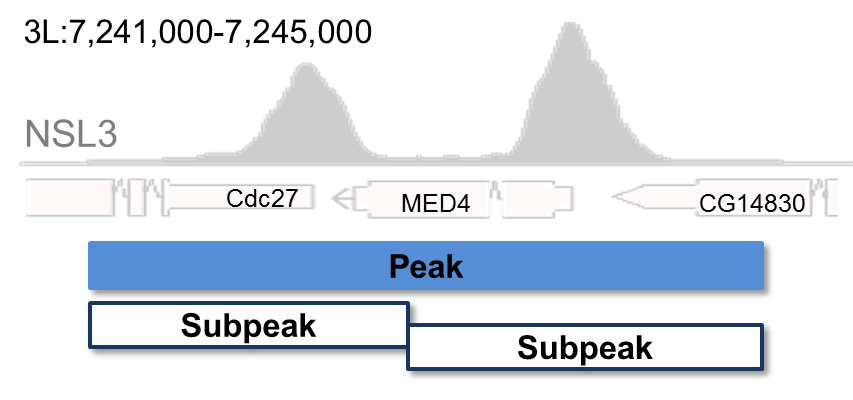
\includegraphics[width=6.5cm,trim=2 2 2 2,clip]{Figures/PeakCalling_Dmel}}
				\end{minipage} 
%\\ [2ex]  \hline \\ [1ex]
\tabularnewline \midrule
%-----------------------
\begin{minipage}[c]{3.5cm}
Pol~II in\\\textit{D.~melanogaster} cells\\(depleted of NSL1 or NSL3)
\end{minipage}
	& \begin{minipage}[c]{4cm}
	the mixed signal of Pol~II (localized, TF-like enrichments around TSS, broad, shallow enrichments along gene bodies) was not well captured by MACS
		\end{minipage}
		& \begin{minipage}[c]{8cm}
\vskip 6pt
				\begin{enumerate}[noitemsep, leftmargin=*]
					\item a symmetric null distribution was fitted to regions with negative enrichments, i.e. where the input signal exceeded the ChIP signal \citep{EBIroutine} (black line)
					\item genomic bins that deviated from the expectation (compare the blue with the black line) were determined as significantly enriched (threshold: q-value $\leq$ 0.05) \\ [2ex]
				\end{enumerate}
\vskip 4pt
			\end{minipage}
				& \begin{minipage}[c]{6.5cm}
						\parbox[c]{1em}{
						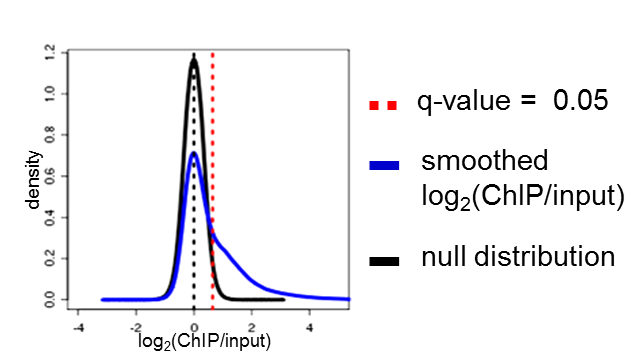
\includegraphics[width=6.5cm,trim=4 4 4 4,clip]{Figures/PeakCalling_PolII}}
					\end{minipage}
%\\ [2ex] \hline \\ [1ex]
\tabularnewline \midrule
%-----------------------
\begin{minipage}[c]{3.5cm}
MOF, MSL1, MSL2,\\NSL3, MCRS1 in\\ mouse ESCs and NPCs
\end{minipage}
	& \begin{minipage}[c]{4cm}
	non-optimal signal-noise ratios, GC bias
		\end{minipage}
		& \begin{minipage}[c]{8cm}
\vskip 6pt
				\begin{enumerate}[noitemsep, leftmargin=*]
                    \item in ESCs: adjustment of the GC bias in the input sample to match each ChIP-seq sample's GC bias
					\item peak calling with MACS 1.4.2 with default parameters \citep{Feng2012} for each ChIP-seq replicate (blue boxes) and the merged file (red box)
					\item only peaks that were present in both replicates and met the FDR threshold of $\leq$ 1\% were used \\ [2ex]
				\end{enumerate}
\vskip 4pt
			\end{minipage}
				& \begin{minipage}[c]{6.5cm}
\vskip 6pt
						\parbox[c]{1em}{
						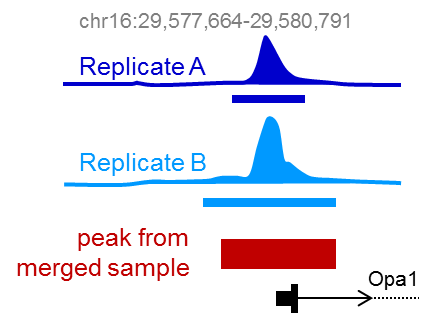
\includegraphics[width=5.5cm,trim=4 4 4 4,clip]{Figures/PeakCalling_Mm}} 
\vskip 4pt
					\end{minipage}
%\\ [2ex] \hline \\ [1ex]
%-----------------------
\tabularnewline \bottomrule
\label{tab:peakCallingStrategies}
\end{longtable}
\end{small}
\end{singlespacing}
\end{landscape}



%=====================
\textbf{APPENDIX}

Lorem ipsum dolor sit amet, consetetur sadipscing elitr, sed diam nonumy eirmod tempor invidunt ut labore et dolore magna aliquyam erat, sed diam voluptua. At vero eos et accusam et justo duo dolores et ea rebum.


CHECKED Tools \\
%\begin{landscape}
\begin{singlespacing}
\begin{small}
%\setlength{\extrarowheight}{15pt} % this doesn't work to control the vertical space
\vspace*{-1em}
\begin{longtable}{>{\textsf\bgroup\raggedleft\arraybackslash}p{2.7cm}<{\egroup} >{\textsf\bgroup}p{4.5cm}<{\egroup} >{\textsf\bgroup}p{4.2cm}<{\egroup}>{\textsf\bgroup}p{2.3cm}<{\egroup}} % defining the columns - these must match the widths defined for the mini pages down below!
\caption[Bioinformatic tools used for analyses presented here.]{\textsf{Bioinformatic tools used for analyses presented here (alphabetical order; if available, I indicated the versions of the tools that I used). For explanations of the file formats mentioned here, please see the glossary within the supplement of \aref{SuppPub_deepTools}.}} \\ % the \\ is important! see http://tex.stackexchange.com/questions/103698/extra-alignment-tab-with-longtable
%%%%%%%%%%%%%%%
% table title
\textbf{Name} & \textbf{Application} & \textbf{Website} & \textbf{Reference}
\tabularnewline \hline
\endfirsthead % indicates that the lines above appear as head of the table on the first page
\multicolumn{4}{c}%
{\tablename\ \thetable\ -- \textit{Continued from previous page}} \\[1ex]
\textbf{Name} & \textbf{Application} & \textbf{Website} & \textbf{Reference}
\tabularnewline \toprule %\tabularnewline [1ex]
\endhead % Line(s) to appear at top of every page (except first)
\multicolumn{4}{r}{\textit{Continued on next page}} \\
\endfoot % Last line(s) to appear at the bottom of every page (except last)
\endlastfoot
%%%%%%%%%%%%%%%%%%%
%% first row
%-----------------------
\toprule %\\ [4ex]
 \begin{minipage}{2.7cm}
				\textbf{bedtools} \\
					(2.10. to 2.17)
				\end{minipage}
			&	 \begin{minipage}{4.5cm}
				working with genomic intervals, e.g. intersecting two files with different peak regions
			\end{minipage} 
			&  \begin{minipage}{4.2cm}
			\url{http://bedtools.readthedocs.org/en/latest/}
			\end{minipage} 
			&  \begin{minipage}{2.3cm}
					\raggedright \citet{Quinlan2010}
				\end{minipage} 
%\\ [4ex] \hline \\ [1ex]
\tabularnewline \midrule
%---------------------------
 \begin{minipage}{2.7cm}
				\textbf{bowtie} \\
					bowtie-1.0.0\\(Appendix \ref{SuppPub_NSL}),\\
					bowtie2-2.2.2\\(Appendix \ref{SuppPub_MSL}) %\\ [2ex]
			\end{minipage} 
			&  \begin{minipage}{4.5cm}
			alignment of reads to the reference genome
				\end{minipage} 
				&  \begin{minipage}{4.2cm}
				\url{http://bowtie-bio.sourceforge.net/index.shtml}
				\end{minipage} 
				&  \begin{minipage}{2.3cm}
				Langmead and\\
				Salzberg \citep{Langmead2012}
			\end{minipage} 
%\\ [4ex] \hline \\ [1ex]
\tabularnewline \midrule
%-----------------------
 \begin{minipage}{2.7cm}
				\textbf{ChIPEnrich}
			\end{minipage} 
			&  \begin{minipage}{4.5cm}
					gene ontology enrichments for target genes identified by ChIP-seq
			\end{minipage} 
			&  \begin{minipage}{4.2cm}
					\url{http://sartorlab.ccmb.med.umich.edu/chip-enrich}
			\end{minipage} 
			&  \begin{minipage}{2.3cm}
				\citet{Welch2014}
			\end{minipage} 
%\\ [4ex] \hline \\ [1ex]
\tabularnewline \midrule
%-----------------------------
 \begin{minipage}{2.7cm}
		\textbf{DAVID}
\end{minipage} 
			&  \begin{minipage}{4.5cm}
				gene identifier mapping and gene ontology term enrichment analyses
			\end{minipage} 
			&  \begin{minipage}{4.2cm}
				\url{http://david.abcc.ncifcrf.gov/}
			\end{minipage} 
				&  \begin{minipage}{2.3cm}
				\citet{Huang2009}
			\end{minipage} 
%\\ [4ex] \hline \\ [1ex]
\tabularnewline \midrule
%-----------------------------
 \begin{minipage}{2.7cm}
					\textbf{deepTools} \\
					(up to 1.5.7) %\\ [2ex]
			\end{minipage} 
			&  \begin{minipage}{4.5cm}
				quality controls of BAM files, normalizations, coverage file generation, visualizations with heatmaps and summary plots %\\ [2ex]
			\end{minipage} 
			&  \begin{minipage}{4.2cm}
				\url{http://deeptools.github.io/} %\\ [2ex]
			\end{minipage} 
				&  \begin{minipage}{2.3cm}
		\raggedright Ramirez, Dündar et al. \citep{Ramirez2014} %\\ [2ex]
			\end{minipage} 
%\\ [4ex] \hline \\ [1ex]
\tabularnewline \midrule
%-----------------------------
 \begin{minipage}{2.7cm}
					\textbf{DESeq}\\
					(1.10.1)
				\end{minipage} 
			&  \begin{minipage}{4.5cm}
				calculating normalized fold change values for Pol~II ChIP-seq data set \citep{EBIroutine}
			\end{minipage} 	
			&  \begin{minipage}{4.2cm}
				\url{http://www-huber.embl.de/users/anders/DESeq/}
			\end{minipage}
				& 
				\begin{minipage}{2.3cm}
		\citet{Anders2010}
			\end{minipage} 
%\\ [4ex] \hline \\ [1ex]
\tabularnewline \midrule
%---------------------------
 \begin{minipage}{2.7cm}
				\textbf{fastqc}
				\end{minipage}
			&  \begin{minipage}{4.5cm}
				quality control of FASTQ files
			\end{minipage} 
			&  \begin{minipage}{4.2cm}
				\url{http://www.bioinformatics.babraham.ac.uk/projects/fastqc/}
			\end{minipage} 
			&  not available
%\\ [4ex] \hline \\ [1ex]
\tabularnewline \midrule
%-----------------------------
 \begin{minipage}{2.7cm}
				\textbf{Galaxy} %%\\ [2ex]
				\end{minipage} 
			&  \begin{minipage}{4.5cm}
				vast collection of tools for manifold tasks including working with genomic intervals, joining of lists, motif search etc. %\\ [2ex]
			\end{minipage} 
			&  \begin{minipage}{4.2cm}
				in-house installation %%\\ [2ex]
			\end{minipage} 
					&  \begin{minipage}{2.3cm}
		\citet{Goecks2010} %%\\ [2ex]
			\end{minipage} 
%\\ [4ex] \hline \\ [1ex]
\tabularnewline \midrule
%-----------------------------
 \begin{minipage}{2.7cm}
					\textbf{ggplot2}\\
					(0.9.3.1)
			\end{minipage} 
			&  \begin{minipage}{4.5cm}
				R package for highly customizable plots (e.g. boxplots, x-y plots, bar charts etc.)
			\end{minipage} 
			&  \begin{minipage}{4.2cm}
				\url{http://ggplot2.org/}
			\end{minipage} 
			&  \begin{minipage}{2.3cm}
		\citet{ggplot2}
			\end{minipage} 
%\\ [4ex] \hline \\ [1ex]
\tabularnewline \midrule
%-----------------------------
 \begin{minipage}{2.7cm}
					\textbf{GREAT}\\
					(2.0)
				\end{minipage} 
			&  \begin{minipage}{4.5cm}
				web-based tool for target gene prediction
			\end{minipage} 
			&  \begin{minipage}{4.2cm}
				\url{http://bejerano.stanford.edu/great/public/html/}
			\end{minipage} 
				&  \begin{minipage}{2.3cm}
		\citet{McLean2010}
			\end{minipage} 
%\\ [4ex] \hline \\ [1ex]
\tabularnewline \midrule
%----------------------------
 \begin{minipage}{2.7cm}
					\textbf{Integrative\\Genomics\\Viewer}\\
					(up to 2.3.32) %\\ [2ex]
			\end{minipage} 
			& 	\begin{minipage}{4.5cm}
				genome browser for visualization of BAM, BED, bigWig and bedGraph files %\\ [2ex]
			\end{minipage} 
			&  \begin{minipage}{4.2cm}
				\url{http://www.broadinstitute.org/igv/} %\\ [2ex]
			\end{minipage} 
				&  \begin{minipage}{2.3cm}
		\citet{Thorvaldsdottir2013} %\\ [2ex]
			\end{minipage} 
%\\ [4ex] \hline \\ [1ex]
\tabularnewline \midrule
%-----------------------------
 \begin{minipage}{2.7cm}
					\textbf{liftover}\\
					(2013)
			\end{minipage} 
			&  \begin{minipage}{4.5cm}
				conversion of sequence coordinates from mm8 assembly to mm9
			\end{minipage} 
			&  \begin{minipage}{4.2cm}
				\url{https://genome.ucsc.edu/cgi-bin/hgLiftOver}
			\end{minipage} 
				&  not available
%\\ [4ex] \hline \\ [1ex]
\tabularnewline \midrule
%-----------------------------
 \begin{minipage}{2.7cm}
				\textbf{MACS}\\
					(1.4.2)
				\end{minipage}
			&	 \begin{minipage}{4.5cm}
				identification of significantly enriched ChIP-seq regions
			\end{minipage} 
			&  \begin{minipage}{4.2cm}
				\url{http://liulab.dfci.harvard.edu/MACS/}
			\end{minipage} 
				&  \begin{minipage}{2.3cm}
		\citet{Zhang2008}
			\end{minipage} 
%\\ [4ex] \hline \\ [1ex]
\tabularnewline \midrule
%-----------------------------
 \begin{minipage}{2.7cm}
				\textbf{MEME}\\
					(4.9.0)
				\end{minipage} 
			&  \begin{minipage}{4.5cm}
				\textit{de novo} DNA motif identification
			\end{minipage}
			&  \begin{minipage}{4.2cm}
				\url{http://meme.nbcr.net/meme/}
			\end{minipage} 
					&  \begin{minipage}{2.3cm}
		\raggedright  \citet{Bailey1994, Machanick2011}
			\end{minipage} 
%\\ [4ex] \hline \\ [1ex]
\tabularnewline \midrule
%-----------------------------
\begin{minipage}{2.7cm}
				\textbf{PeakSplitter}\\
					(1.0)
				\end{minipage} 
			&  \begin{minipage}{4.5cm}
				splitting peak regions predicted by MACS into separate regions based on local minima detection
			\end{minipage} 
			&  \begin{minipage}{4.2cm}
				\url{http://www.ebi.ac.uk/research/bertone/software}
			\end{minipage} 
			&  \begin{minipage}{2.3cm}
		\citet{Salmon2010}
			\end{minipage} 
%\\ [4ex] \hline \\ [1ex]
\tabularnewline \midrule
%-----------------------------
 \begin{minipage}{2.7cm}
					\textbf{samtools}\\
					(0.1.19)
			\end{minipage} 
			&	 \begin{minipage}{4.5cm}
				SAM and BAM file handling (indexing, number of mapped/unmapped and uniquely reads etc.)
			\end{minipage} 
			&  \begin{minipage}{4.2cm}
				\url{http://samtools.sourceforge.net/}
			\end{minipage} 
				&  \begin{minipage}{2.3cm}
		\citet{Li2009}
			\end{minipage} 
%\\ [4ex] \hline \\ [1ex]
\tabularnewline \midrule
%-----------------------------
 \begin{minipage}{2.7cm}
					\textbf{TRAP}\\
					(Annotate v3.04)
				\end{minipage} 
			&  \begin{minipage}{4.5cm}
				transcription factor binding affinity calculation
			\end{minipage} 
			&  \begin{minipage}{4.2cm}
				\url{http://trap.molgen.mpg.de/PASTAA.htm}
			\end{minipage} 
				&  \begin{minipage}{2.3cm}
		\citet{Roider2007}
			\end{minipage} 
%\\ [4ex] \hline \\ [1ex]
\tabularnewline \midrule
%-----------------------------
 \begin{minipage}{2.7cm}
				\textbf{UCSC tools} \\
					(2013)
				\end{minipage} 
			&  \begin{minipage}{4.5cm}
				format conversion (bedGraph to bigWig)
			\end{minipage} 
			&  \begin{minipage}{4.2cm}
				\url{http://www.broadinstitute.org/igv/}
			\end{minipage} 
					&  \begin{minipage}{2.3cm}
		\citet{Kent2010}
			\end{minipage} 
%\\ [4ex] \hline \\ [1ex]
\tabularnewline \midrule
%-----------------------------
 \begin{minipage}{2.7cm}
				\textbf{Venny}\\
					(2007)
				\end{minipage} 
			& 	\begin{minipage}{4.5cm}
				generation of Venn diagrams
			\end{minipage} 
			&  \begin{minipage}{4.2cm}
				\url{http://bioinfogp.cnb.csic.es/tools/venny/}
			\end{minipage} 
			&  not available
%\\ [4ex] \hline \\ [1ex]
\tabularnewline \bottomrule
%-----------------------------
\label{tab:tools}
\end{longtable}
\end{small}
\end{singlespacing}
%\end{landscape}



CHECK Databases \\
\begin{minipage}{\textwidth} % to avoid pagebreaks despite longtable environment
\begin{singlespacing}
\begin{small}
\setlength{\extrarowheight}{2pt}
%\vspace*{-2em}
\begin{longtable}[l]{>{\textsf\bgroup}p{2cm}<{\egroup} >{\textsf\bgroup}p{6cm}<{\egroup} >{\textsf\bgroup}p{6cm}<{\egroup}} % defining the columns - these must match the widths defined for the mini pages down below!
\caption[Publicly available data bases that were used.]{\textsf{Publicly available data bases that were used.}} \\ % the \\ is important!
%%%%%%%%%%%%%%%
% table title
\textbf{Name} & \textbf{Application} & \textbf{Website}
\tabularnewline
%-----------------------
\toprule
 ArrayExpress & up- and download of high-throughput sequencing data (only raw read files) & \url{http://www.ebi.ac.uk/arrayexpress/} 
\tabularnewline \midrule
%--------------------------
 BioMart & mapping of gene and transcripts between different annotations for genome version mm9, e.g. Ensembl and RefSeq; download of non-protein-coding transcripts & \url{http://may2012.archive.ensembl.org/biomart/martview/} 
\tabularnewline \midrule
%--------------------------
 FlyBase & download of gene lists and genome sequence & \url{http://flybase.org/} 
\tabularnewline \midrule
%--------------------------
GEO & up- and download of high-throughput sequencing data (raw and processed data) & \url{http://www.ncbi.nlm.nih.gov/geo/} 
\tabularnewline \midrule
%--------------------------
HomoloGene & list of orthologous genes in \textit{Drosophila}, mice and humans & \url{http://www.ncbi.nlm.nih.gov/homologene} 
\tabularnewline \midrule
%--------------------------
\raggedright UCSC Table Browser & RefSeq gene lists, mappability tracks, GC content tracks, mouse DNase hypersensitivity tracks & \url{https://genome.ucsc.edu/}
%--------------------------
\tabularnewline \bottomrule
%-----------------------------
\label{tab:DB}
\end{longtable}
\end{small}
\end{singlespacing}
\end{minipage}


%NSLcomplexNew\\
%\begin{landscape}
\begin{longtable}{>{\textsf\bgroup}p{2.5cm}<{\egroup} >{\textsf\bgroup}p{16cm}<{\egroup}} % defining the columns - these must match the widths defined for the mini pages down below!
\caption{The NSL complex is composed of evolutionarily conserved proteins that are largely uncharacterized in \textit{D. melanogaster} (n.a. – no information available).} \\
%%%%%%%%%%%%%%%
% table title
\textbf{Protein} & \textbf{Known biological functions}
\tabularnewline \hline
\endfirsthead % indicates that the lines above appear as head of the table on the first page
\multicolumn{2}{c}%
{\tablename\ \thetable\ -- \textit{Continued from previous page}} \\
\textbf{Protein} & \textbf{Known biological functions}
\endhead % Line(s) to appear at top of every page (except first)
\hline \multicolumn{2}{r}{\textit{Continued on next page}} \\
\endfoot % Last line(s) to appear at the bottom of every page (except last)
\endlastfoot
%%%%%%%%%%%%%%%%%%%
%%% let's start the table content; each column (often) gets its own minipage which enables itemized lists etc.
%%%%%%%%%%%%%%%%%%%
\begin{minipage}{2.5cm} % 1st column
				%\vskip 6pt
					\textbf{NSL1} \\
					hMSL1vs, Kansl1
				%\vskip 4pt
			\end{minipage}
				& \begin{minipage}{16cm} % 2nd column
					%	\vskip 6pt
						\begin{itemize}[noitemsep]
							\item interacts with MOF via PEHE domain [7, 18] \\
							\item Kansl1 conveys acetylation of H4K16 and p53 through MOF interaction [Li, 2009]
							\item interacts with WDR5
							\item \textit{Kansl1} haploinsufficiency causes core phenotype of 17q21.31 microdeletion syndrome [24, 25]
						\end{itemize}				
						\vskip 4pt
					\end{minipage}
\tabularnewline \hline  % new row
%-----------------------
\begin{minipage}{2.5cm}
				\vskip 6pt
					\textbf{NSL2} \\
					Kansl2
				\vskip 4pt
			\end{minipage}
						& n.a
\tabularnewline \hline
%-----------------------
\begin{minipage}{2.5cm}
				\vskip 6pt
					\textbf{NSL3} \\
					KIAA1310 \\
					Kansl3
				\vskip 4pt
			\end{minipage}
					& \begin{minipage}{16cm}
						\vskip 6pt
						\begin{itemize}[noitemsep]
							\item can activate gene expression
						\end{itemize}				
						\vskip 4pt
					\end{minipage}
\tabularnewline \hline
%-----------------------
\begin{minipage}{2.5cm}
				\vskip 6pt
					\textbf{MCRS2} \\
					MSP58 \\
					Mcrs1
				\vskip 4pt
			\end{minipage}
					& \begin{minipage}{16cm}
						\vskip 6pt
						\begin{itemize}[noitemsep]
							\item interaction with Pol II machinery [20]
							\item mammalian Msp58 suggested in nucleolar protein trafficking and rRNA gene transcription enhancement [26]
							\end{itemize}				
						\vskip 4pt
					\end{minipage}
\tabularnewline \hline
%-----------------------
\begin{minipage}{2.5cm}
				\vskip 6pt
					\textbf{MBD-R2} \\
					Phf20
				\vskip 4pt
			\end{minipage}
				& \begin{minipage}{16cm}
						\vskip 6pt
						\begin{itemize}[noitemsep]
							\item general transcription activator [21]
							\item binds histone (di)methyl lysine [27]
							\item \textit{Phf20} ko mice die perinatally with skeletal and hematopoietic abnormalities [28]
							\item antigen against PHF20 is frequently expressed in glioma
						\end{itemize}				
						\vskip 4pt
					\end{minipage}
\tabularnewline \hline
%-----------------------
\begin{minipage}{2.5cm}
				\vskip 6pt
					\textbf{WDS} \\
					Wdr5 \\
				\vskip 4pt
			\end{minipage}
					& \begin{minipage}{16cm}
						\vskip 6pt
						\begin{itemize}[noitemsep]
							\item WD repeats suggest multiple protein interactions [30]
							\item part of several mammalian methyl transferase complexes (MLL, ATAC [23,31,32])
							\item interacts with SRY yo activate Sox9 expression in human prostate cell line [33]
							\item Wdr5 expression correlates with undifferentiated state of embryonic stem cells [34]
						\end{itemize}				
						\vskip 4pt
					\end{minipage}
\tabularnewline \hline %\end{table}
%-----------------------
\label{tab:NSL}
\end{longtable}
\end{landscape}




%----------------------------------------------------------------------------------------
%	THESIS CONTENT - APPENDICES
%----------------------------------------------------------------------------------------

\addtocontents{toc}{\vspace{2em}} % Add a gap in the Contents, for aesthetics

\appendix % Cue to tell LaTeX that the following 'chapters' are Appendices

% Include the appendices of the thesis as separate files from the Appendices folder

% Appendix Template

\definecolor{Light}{gray}{.85}
\newcommand{\overbox}[2][l]{%
  \colorbox{Light}{\begin{tabular}{@{}#1@{}}#2\end{tabular}}%
}

\chapter{Publications and manuscripts} % Main appendix title
%
%===================================================
%%%%%%%%%%%%%%%%%%%%%%%% NSL in D.mel
\fancyhead{}
\fancyhead[RO,LE]{Appendix: \emph{Lam, M{\"u}hlpfordt, Vaquerizas et al. (2012), PLoS Genetics.}}
\fancyfoot[C]{\thepage}

\section{The NSL complex regulates housekeeping genes.}
\label{SuppPub_NSL} % for referencing this appendix elsewhere, use \aref{SuppPub_NSL}

\begin{center}
\noindent\overbox[c]{
Lam,\:K.\:C.*, \textbf{M{\"u}hlpfordt,\:F.*}, Vaquerizas,\:J.\:M.*, Raja,\:S.\:J., Holz,\:H.,\\
Luscombe,\:N.\:M., Manke,\:T., Akhtar,\:A. (2012). \textit{PLoS Genetics}, 8(6), e1002736.\\
doi:10.1371/journal.pgen.1002736 \\
* shared authorship}
\end{center}

I performed the majority of the bioinformatic analyses such as peak calling optimization 
and all further downstream analyses for all ChIP-seq samples. For the ChIP-seq samples of RNA Polymerase II, I additionally performed the read alignment and normalization procedures. 

I generated all figures except Figures 1C, 2D, 3B, 5 and Supplementary Figures 3--6. 

Together with Ken Lam and Asifa Akhtar I devised, wrote, and revised the manuscript.

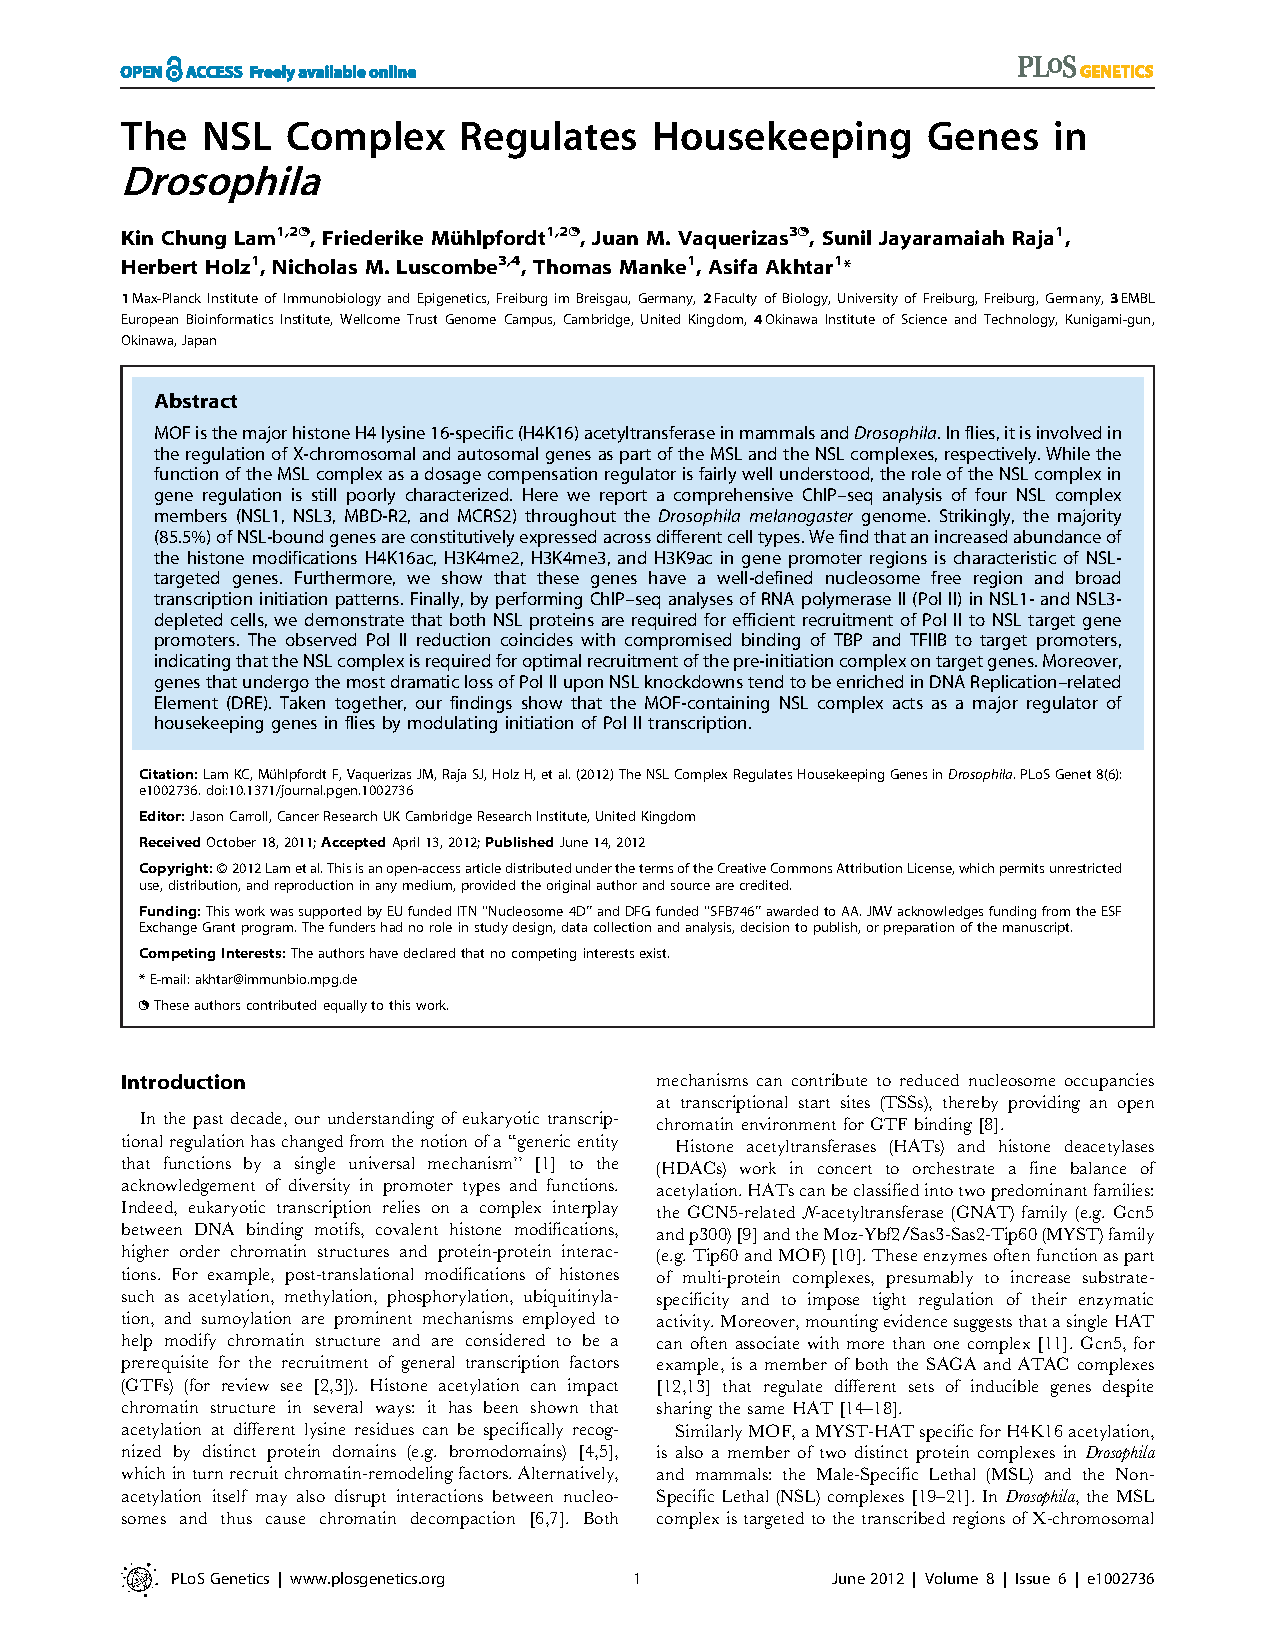
\includepdf[scale=0.9,pages=-,pagecommand={}, offset=0.3cm 0cm]{Figures/Appendix/LamMuhlpfordt2012.pdf} % draft can be added as an option to avoid printing the original pdf; pages=- will include all pages

\subsection{Supplemental Material}
\fancyhead[RO,LE]{Appendix: Supplement to \emph{Lam, M{\"u}hlpfordt, Vaquerizas et al. (2012), PLoS Genetics.}}
\begin{figure}[!h]
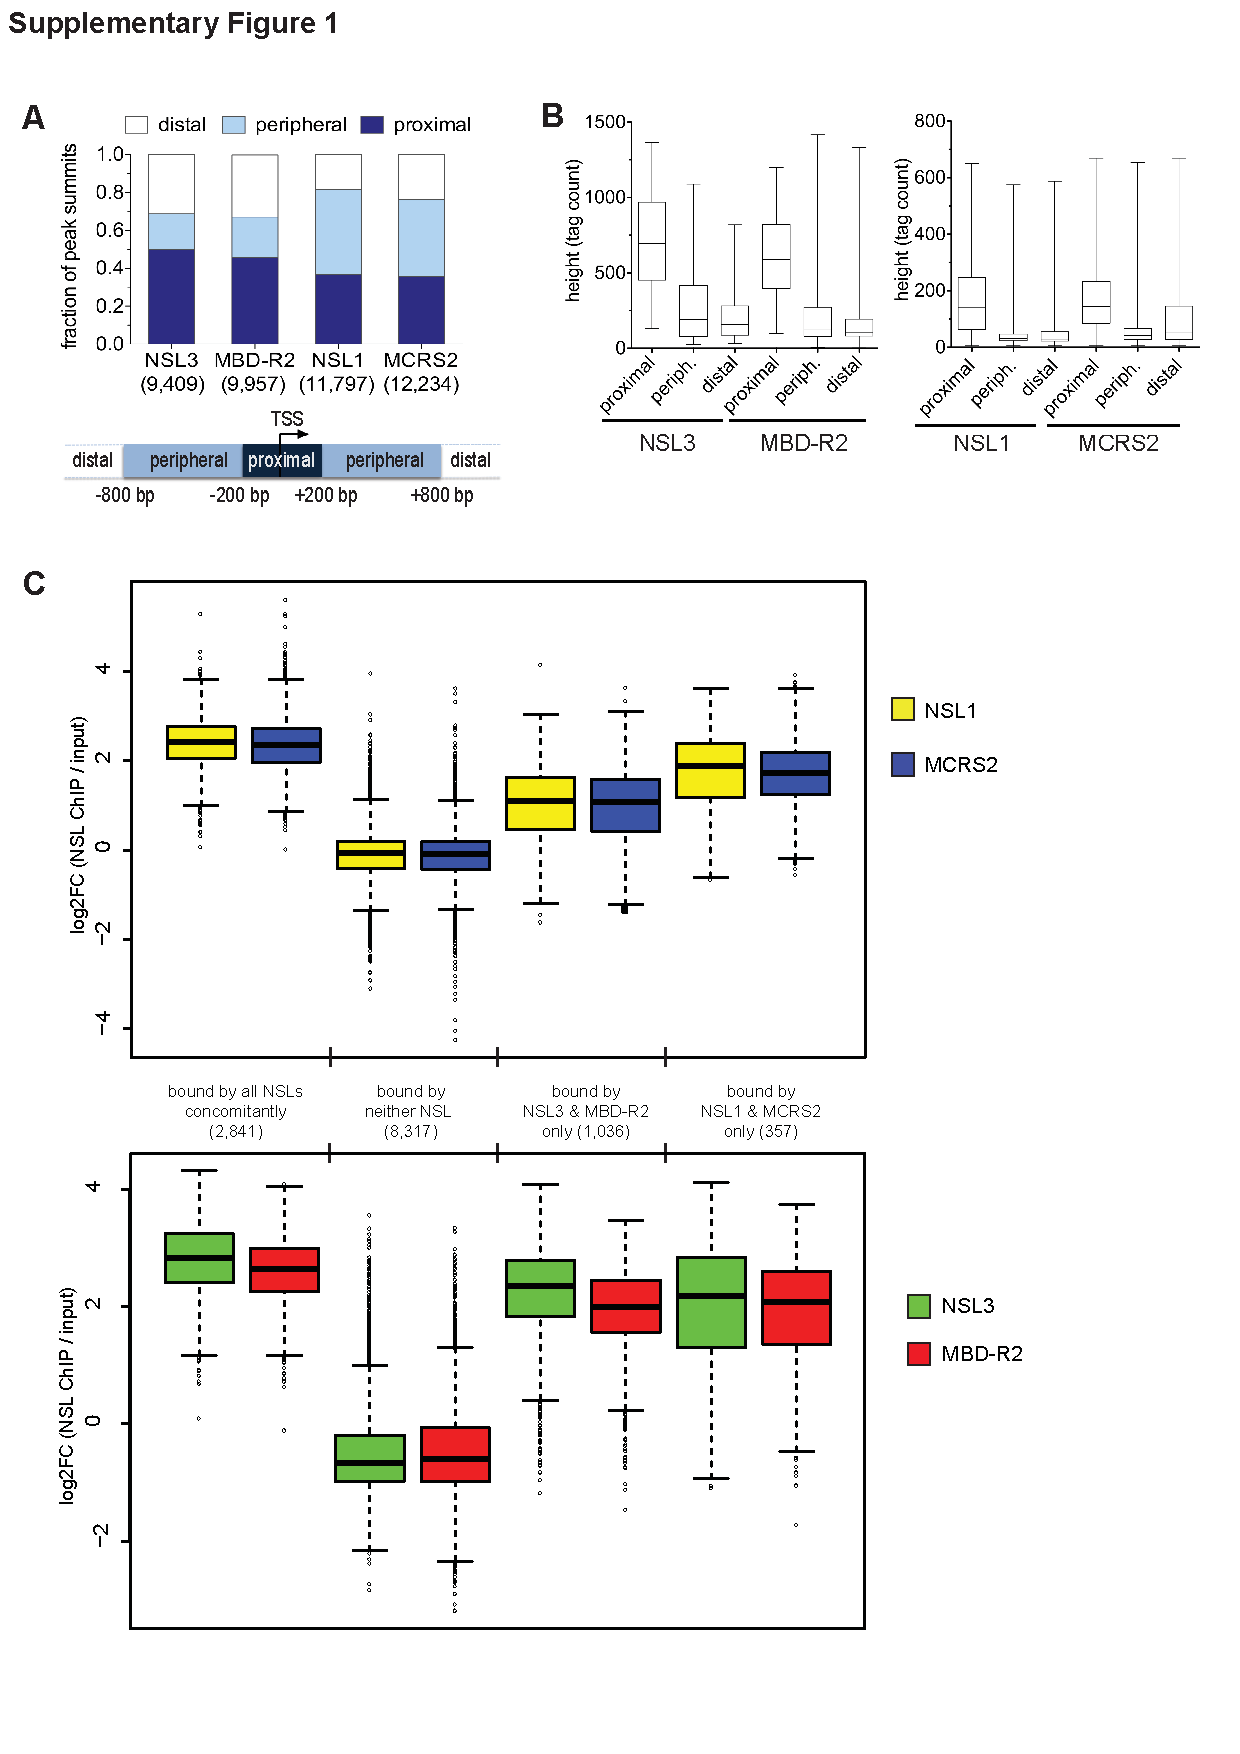
\includegraphics[width=.95\textwidth]{Figures/Appendix/LamMuhlpfordt2012_SupplementP1.pdf}
\end{figure}

\newpage

% INCLUDE THE FIRST PAGE OF THE SUPPLEMENT AS AN IMAGE SO THAT THE HEADER IS NOT ON ITS OWN PAGE
\includepdf[scale=0.8,pages={2-last},pagecommand={},offset=0.3cm 0cm]{Figures/Appendix/LamMuhlpfordt2012_Supplement.pdf} % pages={2-last} will include 2nd to last page

%===================================================
%%%%%%%%%%%%%%%%%%%%%%%% ELIFE
\fancyhead[RO,LE]{Appendix: \emph{Chelmicki, D{\"u}ndar et al. (2014), eLife.}}
\section{MOF-associated complexes ensure stem cell identity and \textit{Xist} repression}
\label{SuppPub_MSL} 

\begin{center}
\noindent\overbox[c]{Chelmicki,\:T.*, \textbf{D{\"u}ndar,\:F*.}, Turley,\:M.\textsuperscript{$\triangle$}, Khanam,\:T.\textsuperscript{$\triangle$}, Aktas,\:T.\textsuperscript{$\triangle$}, \\
Ramírez,\:F., Gendrel,\:A.\:V., Wright,\:P.\:R., Videm,\:R., Backofen,\:R.,\\
Heard,\:E., Manke,\:T., Akhtar,\:A. (2014). eLife. doi:10.7554/eLife.02024 \\
*, \textsuperscript{$\triangle$} shared authorship}
\end{center}

I performed all bioinformatic analyses except the mapping of the RNA-seq data and the determination of differentially expressed genes with DESeq2 which was done by Patrick Wright and Pavan Videm.

I generated all figures except Figures 1, 2G, 3F, 5--7 and the corresponding Supplementary Figures. I contributed to Figure 8. 

Together with Tomasz Chelmicki and Asifa Akhtar I devised, wrote, and revised the manuscript. 

\includepdf[scale=0.9,pages=-,pagecommand={}]{Figures/Appendix/ChelmickiDundar2014.pdf} % removed ,offset=75 -75 after replacing vmargin in thesis cls with geometry package
%
\subsection{Supplemental Material}
\fancyhead[RO,LE]{Appendix: Supplement to \emph{Chelmicki, D{\"u}ndar et al. (2014), eLife.}}
%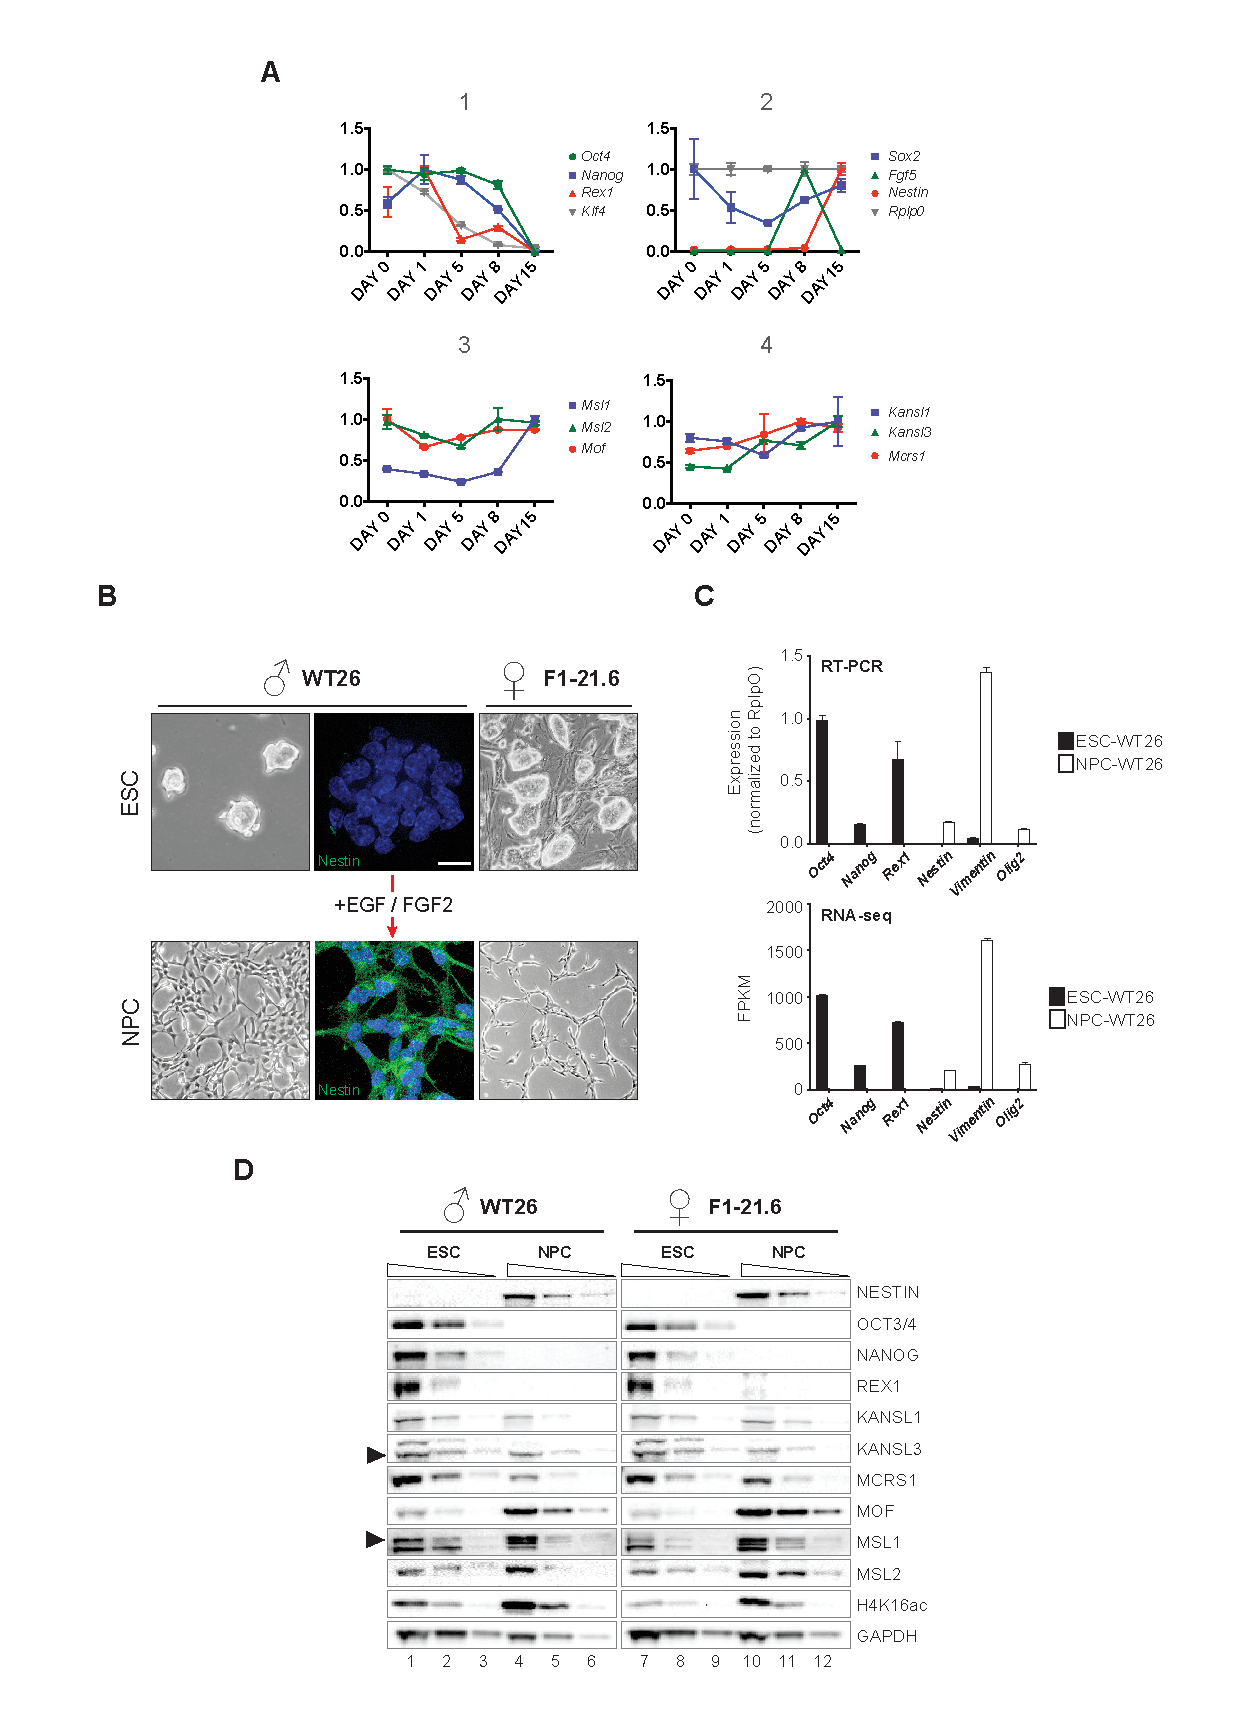
\includegraphics[width=1\textwidth]{Figures/Appendix/Figure1_supplemental_figure1.pdf}
\begin{footnotesize}
\begin{sffamily}
\begin{singlespacing}

%%%%%%%%%%%%%%%%%%%%%%%%%%%%%%%%%%%
% 1-1
%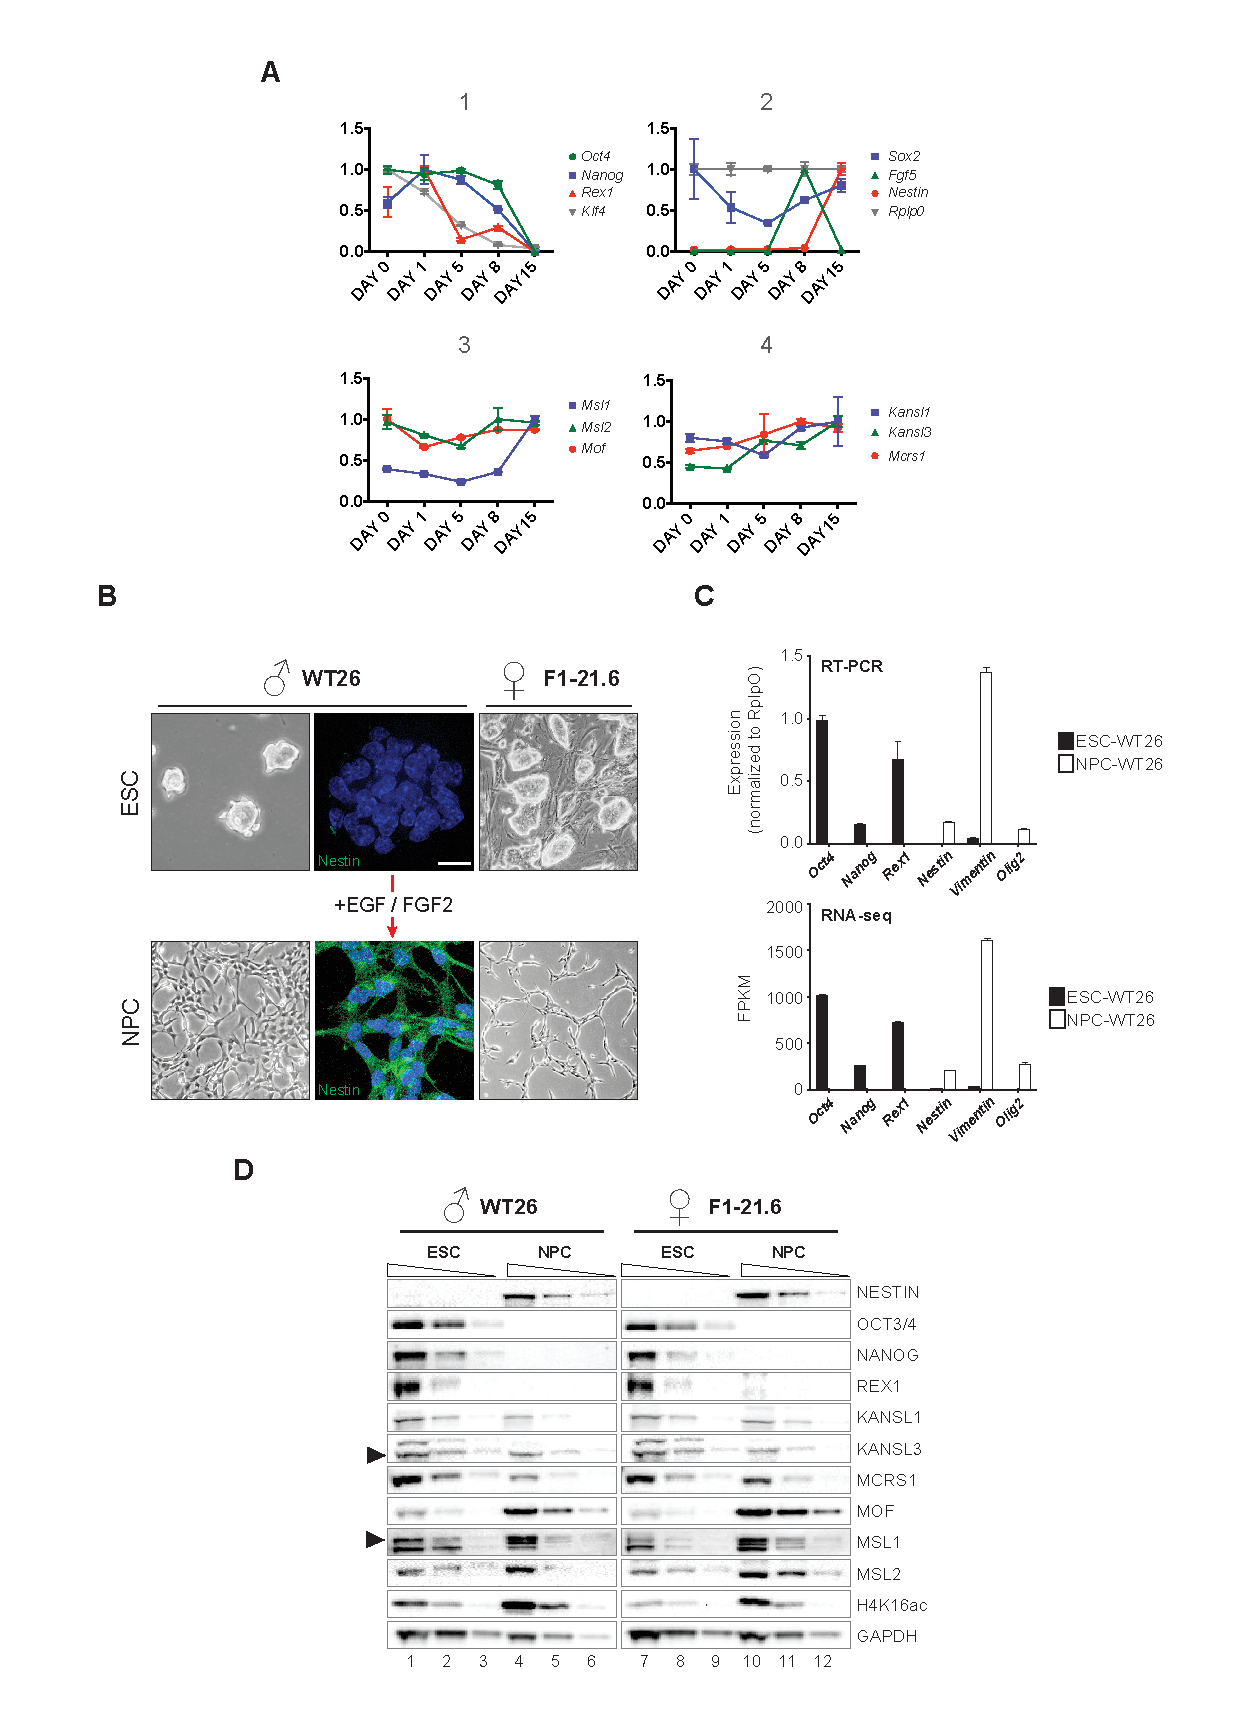
\includepdf[scale=0.9, pages={1}, pagecommand={}, offset=75 -75]{Figures/Appendix/Figure1_supplemental_figure1.pdf}
\textbf{Figure 1—figure supplement 1: Monitoring RNA and protein levels in ESCs and NPCs.
}

A) We monitored the expression dynamics during ESC differentiation for markers of pluripotency (\textit{Oct4, Nanog, Rex1, Klf4}), embryoid body formation (\textit{Fgf5}), differentiation (\textit{Sox2}), and NPC (\textit{Nestin}). Panels 3 and 4 contain the expression profiles for members of the MSL complex (\textit{Msl1, Msl2}), Mof, and the NSL complex (\textit{Kansl1, Kansl3, Mcrs1}), respectively. All results are represented as relative values individually normalized to Rplp0 expression levels (panel 2) on a given day and to the highest expression level of a given gene during the entire differentiation process (highest expression level of each gene = 1). The x-axes show days of differentiation. All results are expressed as means +/- S.D. for technical replicates. For primers see Supplementary File 3C.

(B) Bright field images illustrate the cell morphology before and after the process of differentiation. The im\-mu\-no\-fluo\-res\-cence analysis indicates the specific staining for the NESTIN protein (green) in neuronal progenitors (NPC); DNA is counter\-stained with DAPI (blue).

(C) Expression changes for selected ESC-specific and NPC-specific markers before and after differentiation of wild-type WT26 cells in using RT-PCR analysis and RNA-seq.

(D) Western blots for proteins from two ES cell lines and their NPC derivatives. Different dilutions were loaded (10\%, 30\%, 10\%) with the order indicated on top of the blots. Anti-GAPDH was used as loading control; arrows indicate the protein of interest.

\newpage
%
%%%%%%%%%%%%%%%%%%%%%%%%%%%%%%%%%%%
% 1-2
\begin{minipage}[c]{0.4\textwidth}
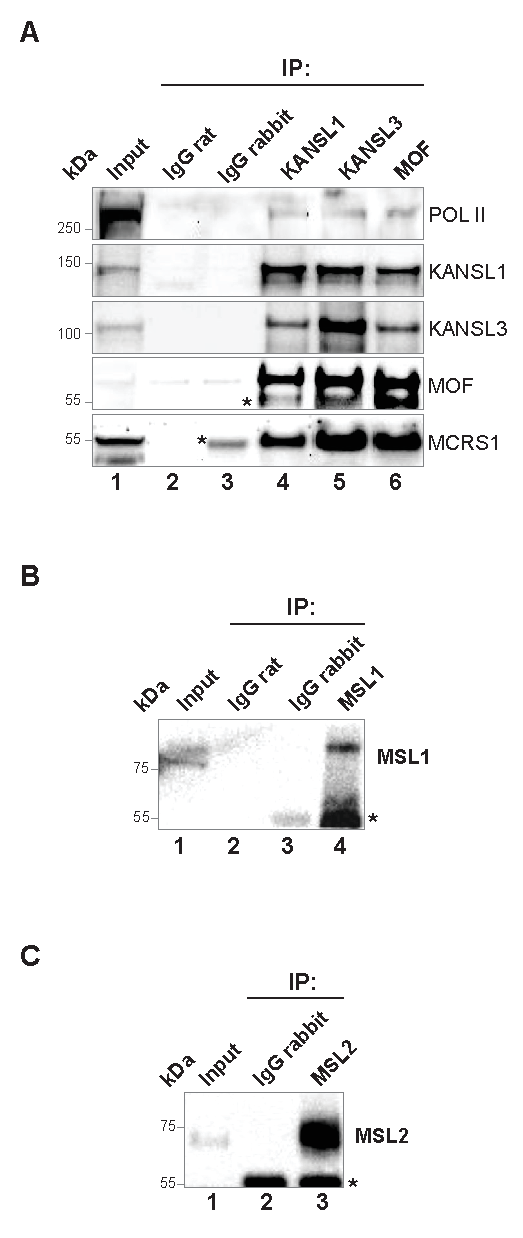
\includegraphics{Figures/Appendix/Figure1_supplemental_figure2_scissored.pdf}
%\caption{\label{fig:blue_rectangle} Rectangle}
\end{minipage} \hfill
\begin{minipage}[c]{0.4\textwidth}
\begin{flushleft}
\textbf{Figure 1—figure supplement 2: Verification of antibodies used in this study.}\tabularnewline \tabularnewline
(A) Immunoprecipitations from mouse ESC nuclear extracts with antibodies specific for KANSL1, KANSL3 or MOF and rabbit or rat antisera. The blot was probed with indicated antibodies showing the co-immunoprecipitation of several NSL complex members. Asterisks represent the IgG signal. Pol II = RNA Polymerase II.\tabularnewline \tabularnewline
(B) and (C) same as (A) except that immunoprecipitations were performed with antibodies specific to MSL1 (B) and MSL2 (C). Asterisks represent the IgG signal.
\end{flushleft}
\end{minipage}
\newpage
%%%%%%%%%%%%%%%%%%%%%%%%%%%%%%%%%%%
% 2-1
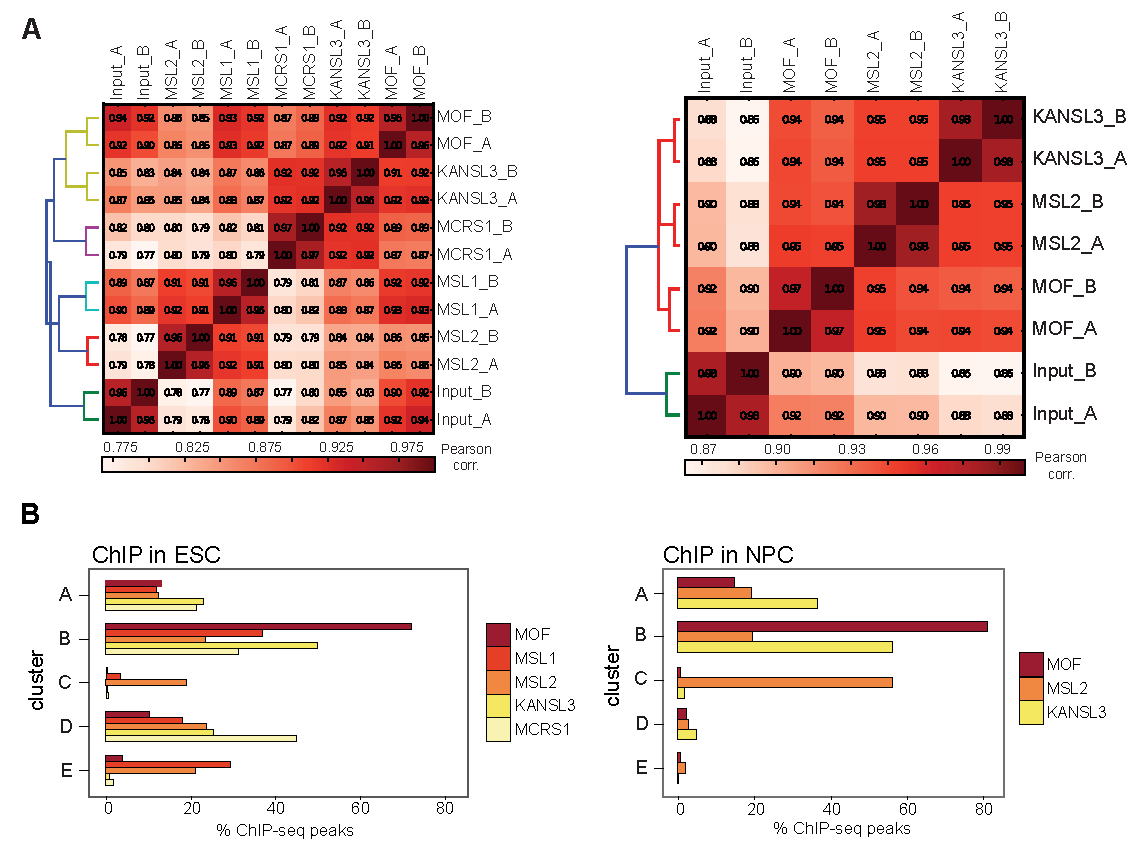
\includegraphics[width=\textwidth]{Figures/Appendix/Figure2_supplemental_figure1_scissored.pdf}

\textbf{Figure 2—figure supplement: ChIP-seq quality measures.}

(A) Correlation plot for all individual ChIP-seq and input samples from ESCs (left) and NPCs. The genome was sampled in windows of 10 kb length; the numbers of reads per bin were counted for each ChIP sample and correlated using Pearson correlation. The calculation and heatmap visualization were done with the bamCorrelate module from the deepTools suite (Ramirez et al., 2014).

(B) The bar chart depicts the fraction of ChIP-seq peaks for each protein that reside within each cluster shown in Figure 2, i.e. approximately 30\% of MSL1 peaks in ESCs locate in cluster E. Note that the absolute numbers of peaks differ between the samples (see Supplementary file 1B for absolute peak numbers and Methods and Materials for peak calling details).
\newpage
%%%%%%%%%%%%%%%%%%%%%%%%%%%%%%%%%%%
% 3-1
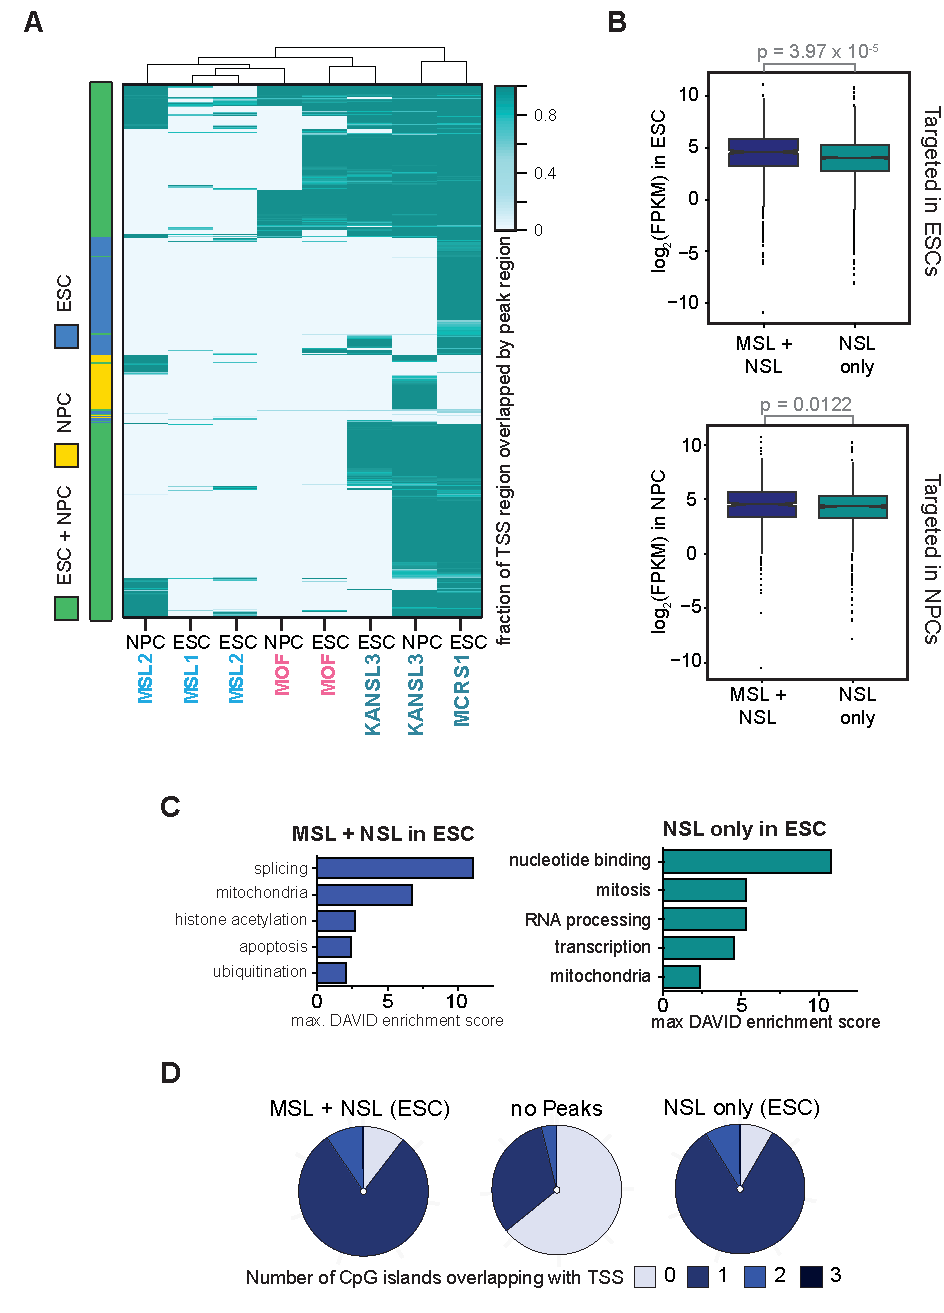
\includegraphics[width=0.77\textwidth]{Figures/Appendix/Figure3_supplemental_figure1_scissored.pdf}

\textbf{Figure 3—figure supplement 1: MSL and NSL complexes target promoters of broadly expressed genes in ESCs and NPCs.
}

(A) The heatmap is related to Figure 3B as it is based on all genes that are bound by at least 1 ChIPed factor in ESCs or NPCs. The intensity of the color depicts the fraction of the 1 kb TSS-region that was covered by a binding site of MOF, MSL1, MSL2, KANSL3 or MCRS1. Rows and columns were sorted using hierarchical clustering on the Euclidean distances of the overlap fractions using R. The left color bar indicates which genes are targeted in 1 or both cell types.

(B) Distribution of expression values from RNA-seq data in ESCs and NPCs for genes targeted by MSL and NSL complex members together or by the NSL complex only. P-values were calculated using Welch t-test.
(C) Results of the GO term analysis using DAVID (Huang da et al., 2009) on genes that were bound at the TSS in ESCs by NSL complex members only or both MSL and NSL complexes.

(D) The pie charts depict how many times annotated TSSs overlapped with a CpG island. The vast majority of genes that were bound in ESCs by MSL and NSL together or by NSL complex members alone overlapped with at least 1 CpG island (dark and medium blue) while approximately 2/3 of the non-target-TSS did not overlap with any CpG island (light blue for 0 CpG islands within the queried regions).
\newpage
%%%%%%%%%%%%%%%%%%%%%%%%%%
% 3-2
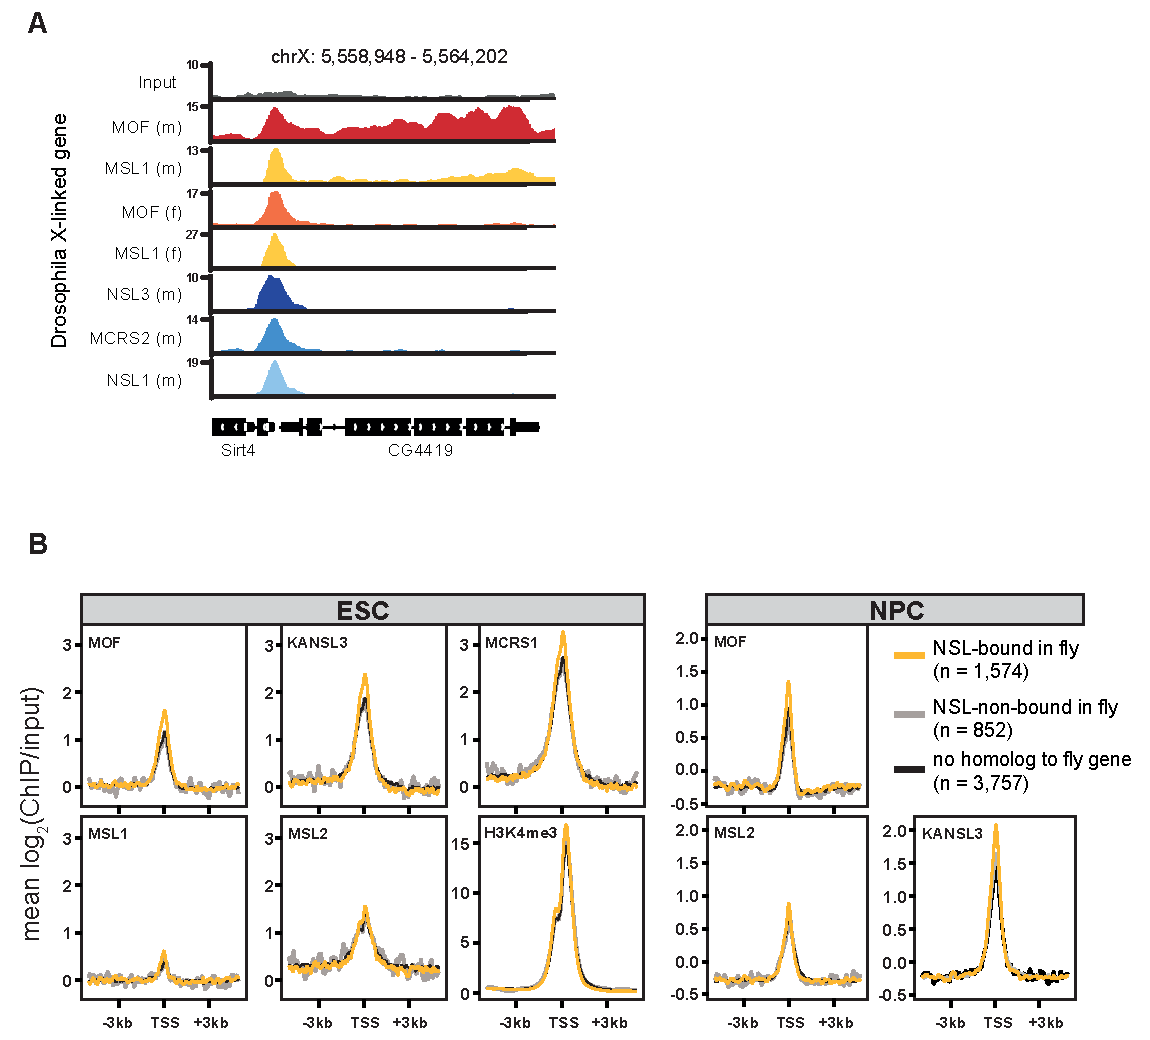
\includegraphics[width=\textwidth]{Figures/Appendix/Figure3_supplemental_figure2_scissored.pdf}

\textbf{Figure 3—figure supplement 2: The NSL-, but not the MSL-binding mode of \textit{D.~me\-la\-no\-gas\-ter} is present in mammalian cells.}

(A) Exemplary genome browser snapshots of the X-linked fly gene CG4419. Shown here are the sequencing-depth normalized profiles for ChIP and corresponding input samples, clearly showing a broad enrichment of MOF and MSL1 along the entire gene body in male (m) \textit{D.~me\-la\-no\-gas\-ter} while all other marks show sharp enrichments around the TSS (including MSL1 and MOF in female (f) \textit{D.~me\-la\-no\-gas\-ter}) which are similar to those seen for both complexes in mouse cells (Figure 3A and 3D).

(B) Comparison of expressed (FPKM \textgreater 4) mouse genes whose homologous genes are either bound or not bound by MOF and its complexes in the fly. We extracted the input-normalized ChIP-seq values for 6~kb regions around the TSS using the computeMatrix module of deepTools (Ramirez et al., 2014). H3K4me3 signal is from a published data set, see Supplementary file 2 for the corresponding accession number.
\newpage
%%%%%%%%%%%%%%%%%%%%%%%%%%
% 3-3
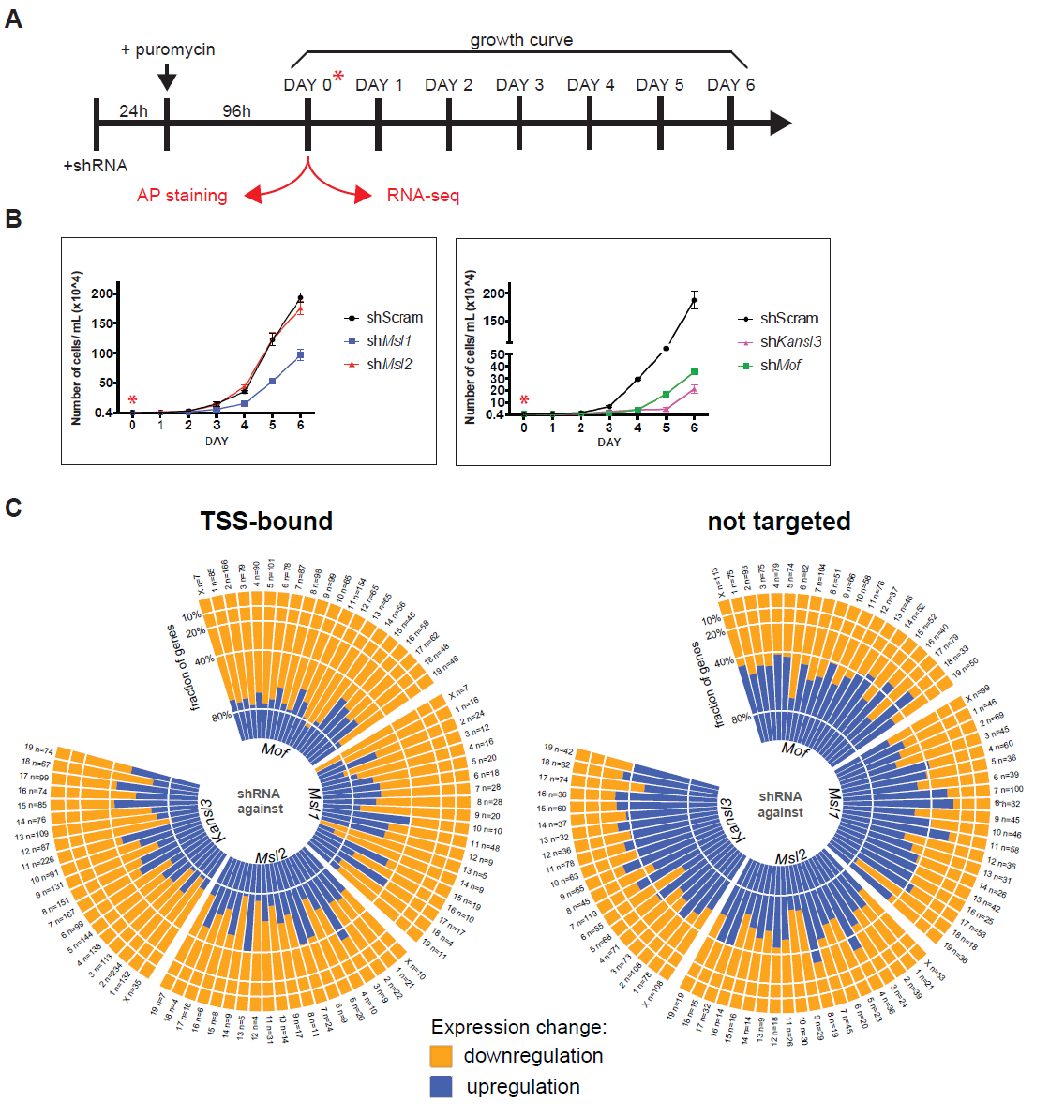
\includegraphics[width=\textwidth]{Figures/Appendix/Figure3_supplemental_figure3_scissored.pdf}

\textbf{Figure 3—figure supplement 3: Effects of shRNA-mediated depletion of MOF, MSL1, MSL2, and KANSL3.}

(A) Time course of knockdown experiments. For experimental details see Methods and Materials. Samples for RNA-sequencing and AP staining (see Figure 4—figure supplement 4) were extracted 4~days after puromycin selection of shRNA-treated cells.

(B) Proliferation assay for shRNA-treated cells, starting at day~4 after puromycin selection (see Figure 3---figure supplement 3A).

(C) Bar plots depicting the fractions of genes (per chromosome) that were significantly up- or downregulated in RNA-seq experiments from shRNA-treated cells. The left plot contains genes which were defined as TSS-targets in the respective ChIP-seq samples, the right plot contains genes that were neither classified as TSS- nor as TSS-distal targets. The labels on each bar indicate the chromosome name and the total number of genes that fulfilled the criteria for this chromosome (significantly affected, TSS-bound or non-targeted). See Methods and Materials for details of the classification.
\newpage
%%%%%%%%%%%%%%%%%%%%%%%%%%
% 3-4
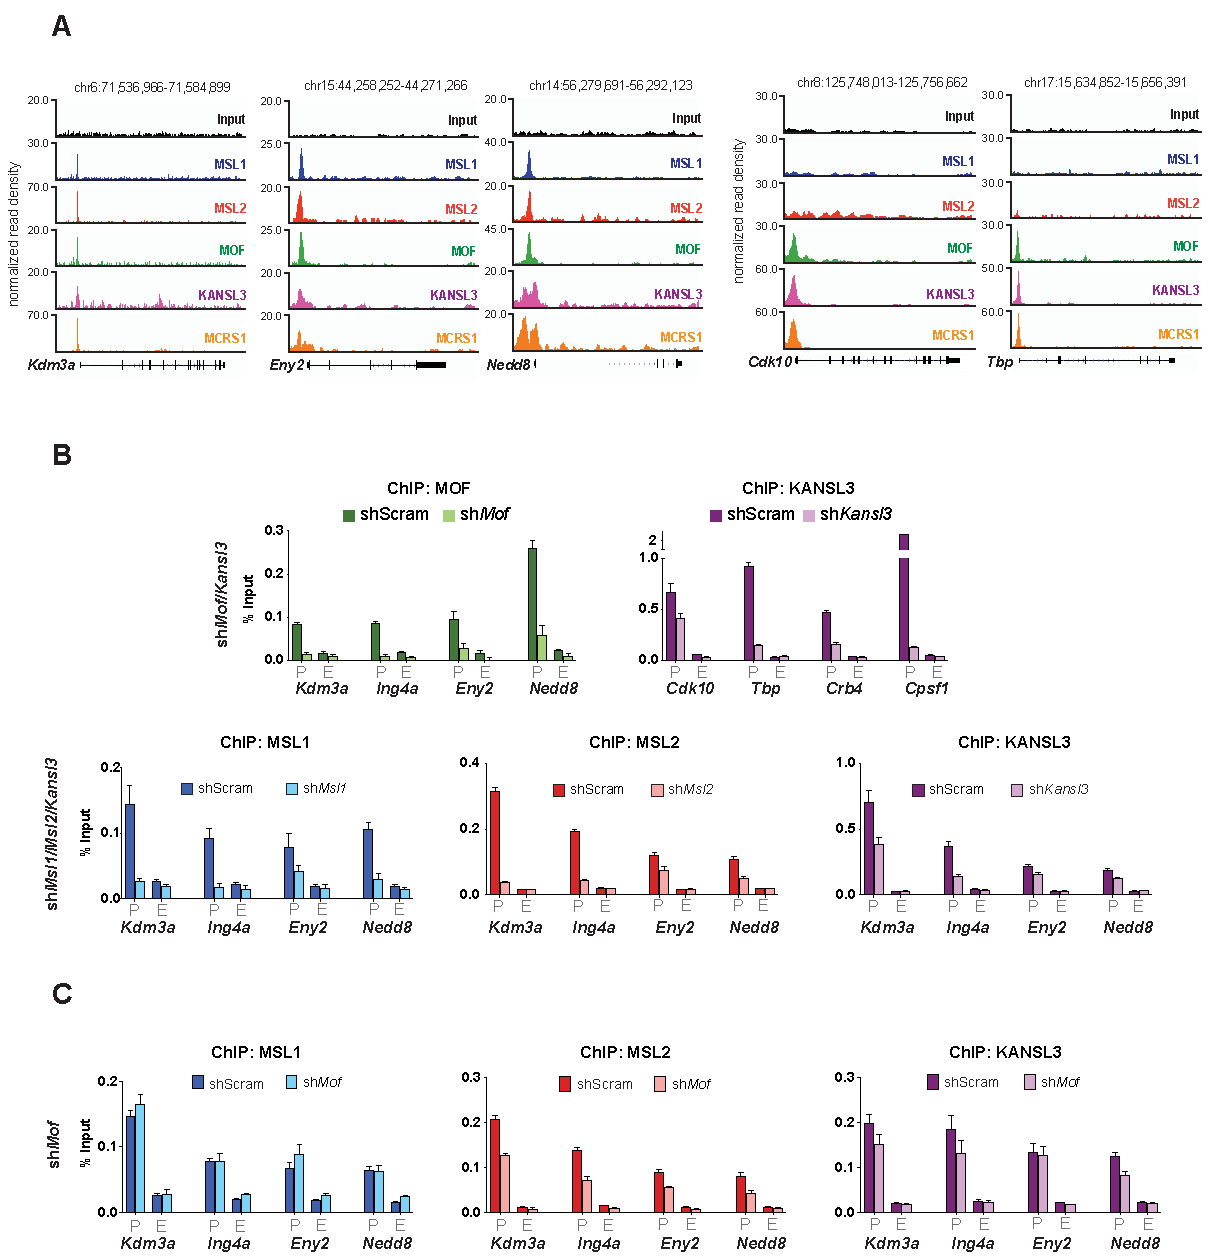
\includegraphics[width=\textwidth]{Figures/Appendix/Figure3_supplemental_figure4_scissored.pdf}

\textbf{Figure 3—figure supplement 4: Assessment of ChIP signals around the TSSs of putative target genes as determined by ChIP-seq.}

(A) Genome Browser snapshots of several MSL/NSL (left) or NSL-only (Visel et al.) target genes and respective sequencing-depth-normalized ChIP-seq and input signals from ESCs. The exact genomic coordinates are indicated on top of each panel. Gene names are indicated on the bottom.

(B) ChIP-qPCR validation for MOF (green) and KANSL3 (purple) signals. Im\-mu\-no\-pre\-ci\-pi\-tated DNA was amplified by qPCR with primer sets positioned at the promoter (P) and end (E) of the coding sequence (Supplementary file 3A). Results are expressed as mean +/- S.D. of 3 biological replicates; cells were harvested for experiments on day~4 (\textit{Kansl3}) or 5 (\textit{Mof}) of knockdown.

(C) ChIP-qPCR for MSL1 (blue), MSL2 (red) and KANSL3 (purple) in ESCs treated with sh-RNA (scrambled or against a specific transcript). Signals on genes were evaluated using primers at the promoter (P), and end (E) of the coding sequence. Results are expressed as mean +/- S.D. of 3~bio\-lo\-gi\-cal replicates; cells were harvested for experiments on day~5 of \textit{Mof} knockdown.
\newpage
%%%%%%%%%%%%%%%%%%%%%%%%%%
% 4-1
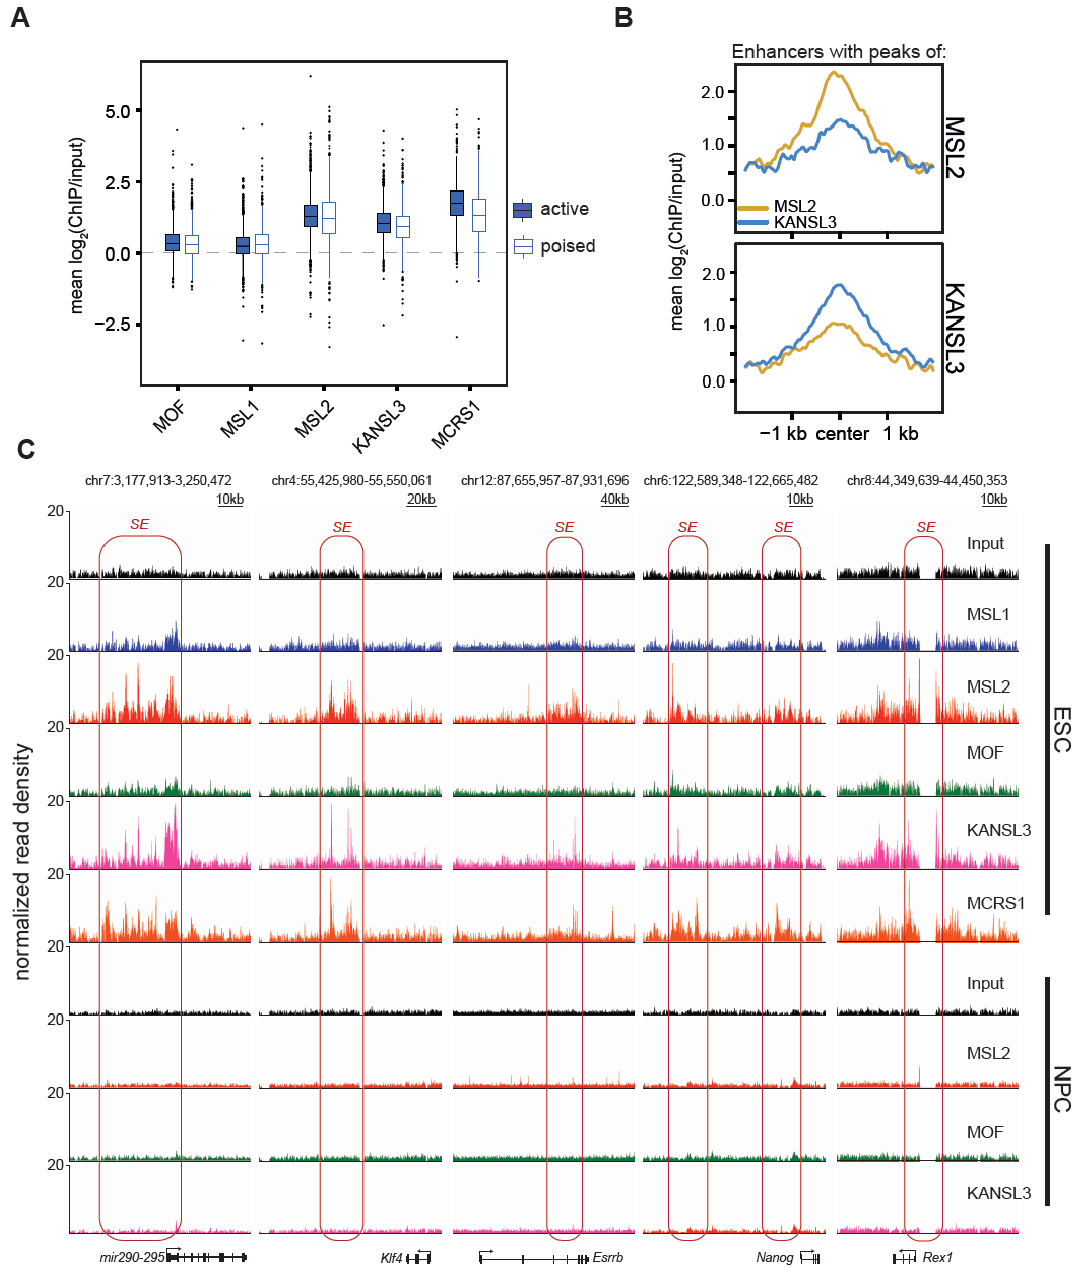
\includegraphics[width=\textwidth]{Figures/Appendix/Figure4_supplemental_figure1_scissored.pdf}

\textbf{Figure 4—figure supplement 1: MSL2 and KANSL3 show strong enrichments at typical and super enhancers in ESCs.}

(A) Boxplots demonstrating the distribution of mean ChIP enrichments for enhancer regions defined by H3K4me1 and H3K27ac marks in ESCs (see Creyghton et al., 2010 for details) that overlap with the clusters of binding defined by our ChIP-seq samples. Mean values were extracting using the UCSCtool bigWigAverageOverBed.

(B) Summary plots for typical enhancer regions (Whyte et al., 2013) that overlapped with either MSL2 (top) or KANSL3 (bottom) peaks. Different colors indicate different ChIP-seq signals. Related to the heatmaps of Figure 4B.

(C) Genome browser snapshots of sequencing-depth normalized ChIP-seq and input profiles for super enhancers of key pluripotency factors.
\newpage
%%%%%%%%%%%%%%%%%%%%%%%%%%
% 4-2
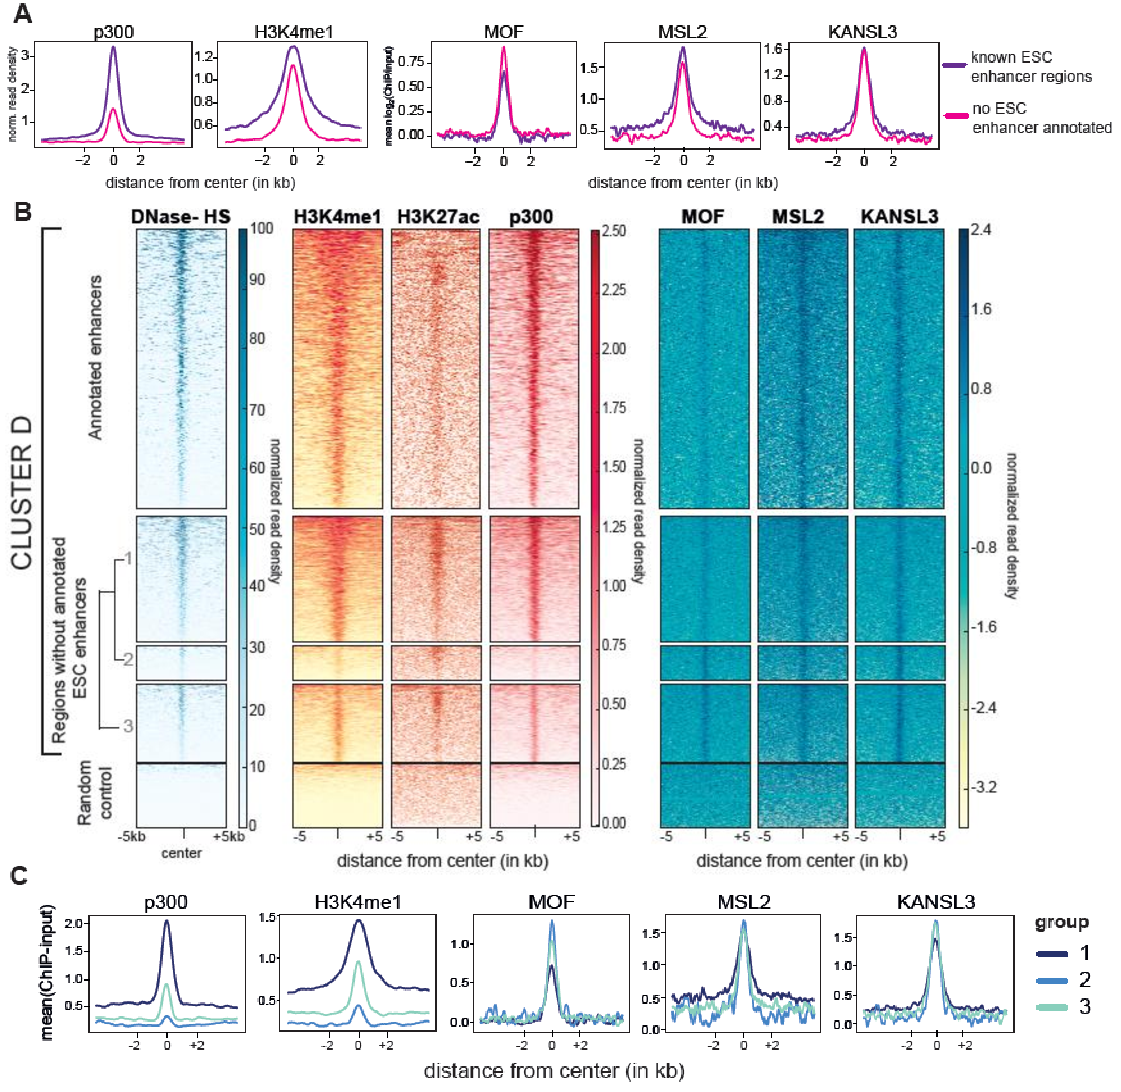
\includegraphics[width=\textwidth]{Figures/Appendix/Figure4_supplemental_figure2_scissored.pdf}

\textbf{Figure 4—figure supplement 2: MOF is moderately enriched at non-canonical enhancers.}

(A) Summary plots of ChIP-seq values for binding sites belonging to cluster D. The regions were divided based on the presence or absence of annotated ESC enhancers (Whyte et al., 2013, Creyghton et al., 2010).

(B) Heatmaps of ChIP-seq read densities of known enhancer markers for the ESC-specific binding sites of our proteins of interest (cluster D, see Figure 2) and random genomic regions. The binding sites of cluster D (excluding regions with TSSs) were divided into 2 basic groups based on the presence or absence of known ESC enhancers (Whyte et al., 2013, Creyghton et al., 2010). The latter group was further divided into 3 (arbitrarily numbered) sub-clusters based on hierarchical clustering of the values from DNase hypersensitivity sites, p300, H3K4me1 and our MOF sample (in ESCs). Heatmaps of the ESC-enhancer-containing regions were sorted according to p300, those of the sub-clustered regions were sorted according to the MOF signal.

(C) Related to (B), shown here are the corresponding summary plots of ChIP-seq values for cluster D binding sites that do not overlap with annotated enhancer regions (bottom part of the heatmaps in the figure above). The 3~indicated groups are based on the hierarchical clustering that was performed on p300, H3K4me1 and MOF values (``Regions without annotated ESC enhancers'' in (B)).
\newpage
%%%%%%%%%%%%%%%%%%%%%%%%%%
% 4-3
\includegraphics[width=\textwidth]{Figures/Appendix/Figure4_supplemental_figure3_scissored.pdf}

\textbf{Figure 4—figure supplement 3: MSL2 has intergenic binding sites in DNA-hypomethylated regions that are enriched for SMAD3 binding sites.}

(A) We extracted the percentage of methylated CpGs and the input-normalized ChIP-seq values from KANSL3 and MSL2 and 5 kb surrounding the center of the regions belonging to cluster C (Figure 2) and random genomic control regions. All heatmaps were sorted according to the percentages of methylated CpGs (Stadler et al., 2011).

(B) Motif obtained by MEME analysis on the top 200 MSL2 peaks within cluster C.

(C) Same as for (A), except that the score was the motif hit score for SMAD3 for 1 kb. See Methods and Materials for details.
\newpage
%%%%%%%%%%%%%%%%%%%%%%%%%%
% 4-4
\includegraphics[width=\textwidth]{Figures/Appendix/Figure4_supplemental_figure4.pdf}

\textbf{Figure 4—figure supplement 4: Biological significance of the TSS-distal binding sites of the investigated proteins.}
\newpage

(A) Genome browser snapshots of sequencing-depth normalized ChIP-seq and input profiles. Pink boxes mark the regions cloned and transfected into ESCs and NPCs for luciferase assays (Figure 4D).

(B) Genes that were significantly up- or downregulated in the respective shRNA-treatments compared to shScrambled were classified according to ChIP-seq peak overlaps (TSS-distal, no target) and expression strength in wild type ESCs (high, intermediate, low). See Methods and Materials for details of the classifications.

(C) Distribution of absolute log2 fold changes (shKansl3 or shMsl2 compared to shScrambled) for significantly downregulated genes. Different shades of orange indicate different target classes based on ChIP-seq experiments for KANSL3 or MSL2, respectively. P-values were calculated with Welch t-test.

(D) Alkaline phosphatase staining and morphology of ESC colonies in indicated knockdowns after 4 days growth under puromycin selection (see Figure 3—figure supplement 3A). MOF- and KANSL3-depleted cells demonstrate reduced alkaline phosphatase positive colonies with increased differentiation compared with MSL1- and MSL2-depleted cells and scrambled control.
\newpage
%%%%%%%%%%%%%%%%%%%%%%%%%%
% 5-1
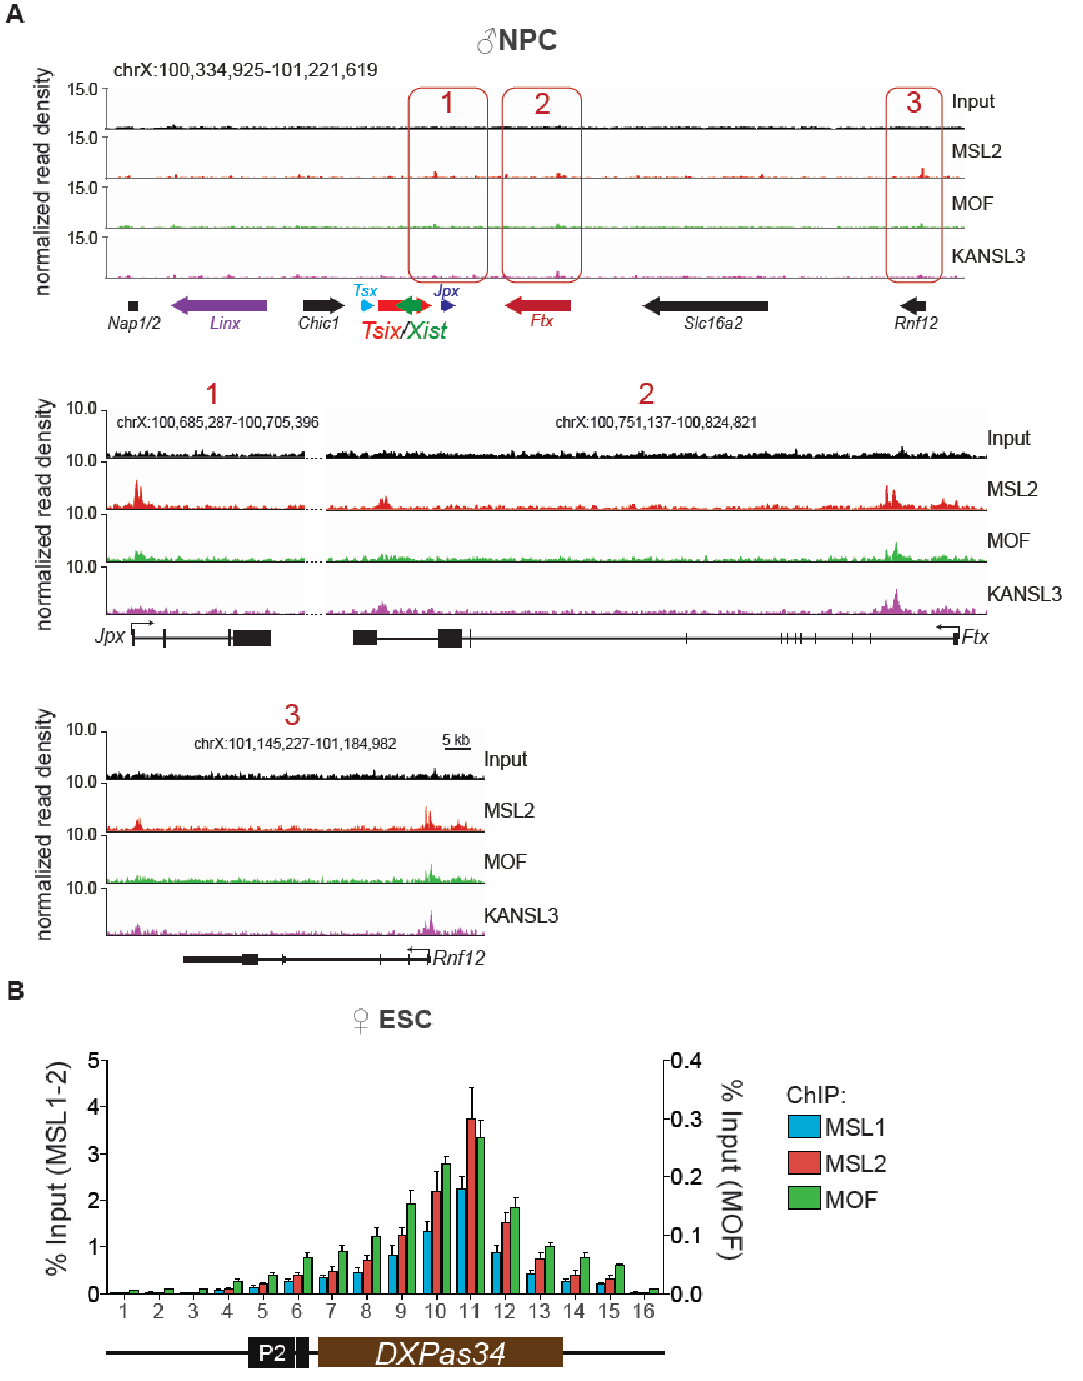
\includegraphics[width=0.9\textwidth]{Figures/Appendix/Figure5_supplemental_figure1_scissored.pdf}

\textbf{Figure 5—figure supplement 1: The MSL proteins bind to multiple loci within the X inactivation center (XIC).}

(A) Genome browser snapshots of the mouse XIC (top panel) with three enlargements on Jpx, Ftx and Rnf12 genes (lower panels). Red boxes with corresponding numbers mark the enlarged regions presented in the lower panels. The exact genomic coordinates are indicated on top of each panel, arrows represent genes. The signals shown are the sequencing-depth normalized ChIP-seq profiles in NPCs.

(B) ChIP analysis of MSL1, MSL2 and MOF across the DXPas34 mini\-sat\-el\-lite in female ESCs. The x-axis labels indicate the genomic coordinates corresponding to the arrowheads in Figure 5A. The y-axes show the percentage of ChIP recovery for MSL1 and MSL2 (left-hand side) and MOF (right-hand side) normalized to input. For all ChIP experiments, 3~biological replicates were used; all results are expressed as mean +/- S.D.
\newpage
%%%%%%%%%%%%%%%%%%%%%%%%%%
% 6-1
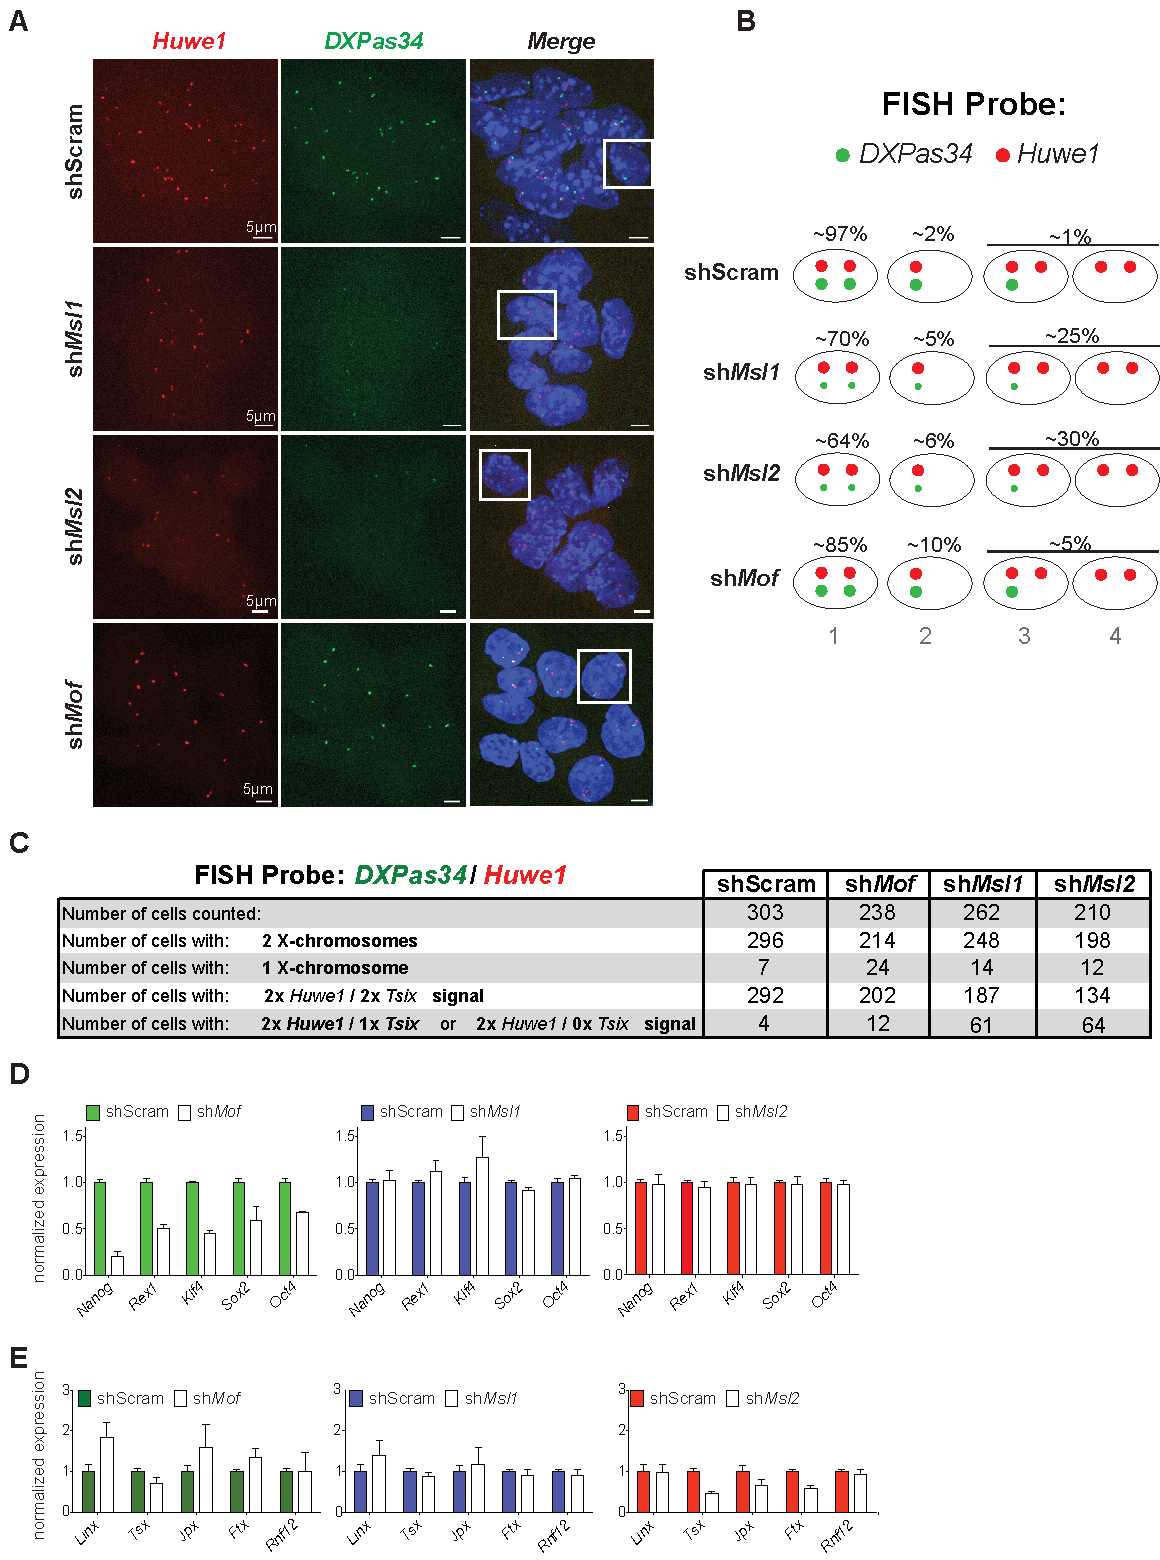
\includegraphics[width=0.9\textwidth]{Figures/Appendix/Figure6_supplemental_figure1_scissored.pdf}

\textbf{Figure 6—figure supplement 1: Cells depleted of MSL1 or MSL2, but not MOF show loss of DXPas34 foci.}

(A) RNA-FISH for \textit{Huwe1} RNA (red) and \textit{DXPas34} RNA (green) in shScrambled-, sh\textit{Msl1}-, sh\textit{Msl2}- and sh\textit{Mof}-treated female ESCs. Shown here are examples of RNA-FISH signals for multicellular colonies and loss of \textit{DXPas34} signal in MSL1- and MSL2-depleted cells. White boxes indicate cells enlarged and resented in Figure 6B. For all experiments, nuclei were coun\-ter\-stained with DAPI (blue).

(B) Summary of RNA-FISH for \textit{DXPas34} and \textit{Huwe1}. Red dots indicate the number of X chromosomes and green dots, \textit{DXPas34} foci (smaller dot = reduced signal). Phenotypes that we observed in knockdowns are categorized into 4 groups containing cells with equal \textit{Huwe1/DXPas34} ratio and with \textit{DXPas34} loss. The percentages indicate how many cells per population showed the respective phenotype.

(C) Corresponding to Figure 6B. Summary of total cell counts from RNA-FISH for (\textit{DXPas34}) and \textit{Huwe1} in MSL1-, MSL2- or MOF-depleted female ESCs.

(D) Gene expression analysis for the indicated genes in female ESCs treated with scrambled RNA (shScram) or shRNA against \textit{Mof}, \textit{Msl1} and \textit{Msl2}. All results are represented as relative values normalized to expression levels in shScram (normalized to \textit{Hprt}) and expressed as means +/- S.D. in 3~biological replicates.

(E) Gene expression analysis for genes of the XIC in female ESCs treated with scrambled RNA or shRNA against \textit{Msl1}, \textit{Msl2} or \textit{Mof}. All results are represented as relative values normalized to expression levels in shScrambled (normalized to \textit{Hprt}) and expressed as means +/- S.D. for 3~biological replicates.
\newpage
%%%%%%%%%%%%%%%%%%%%%%%%%%
% 7-1
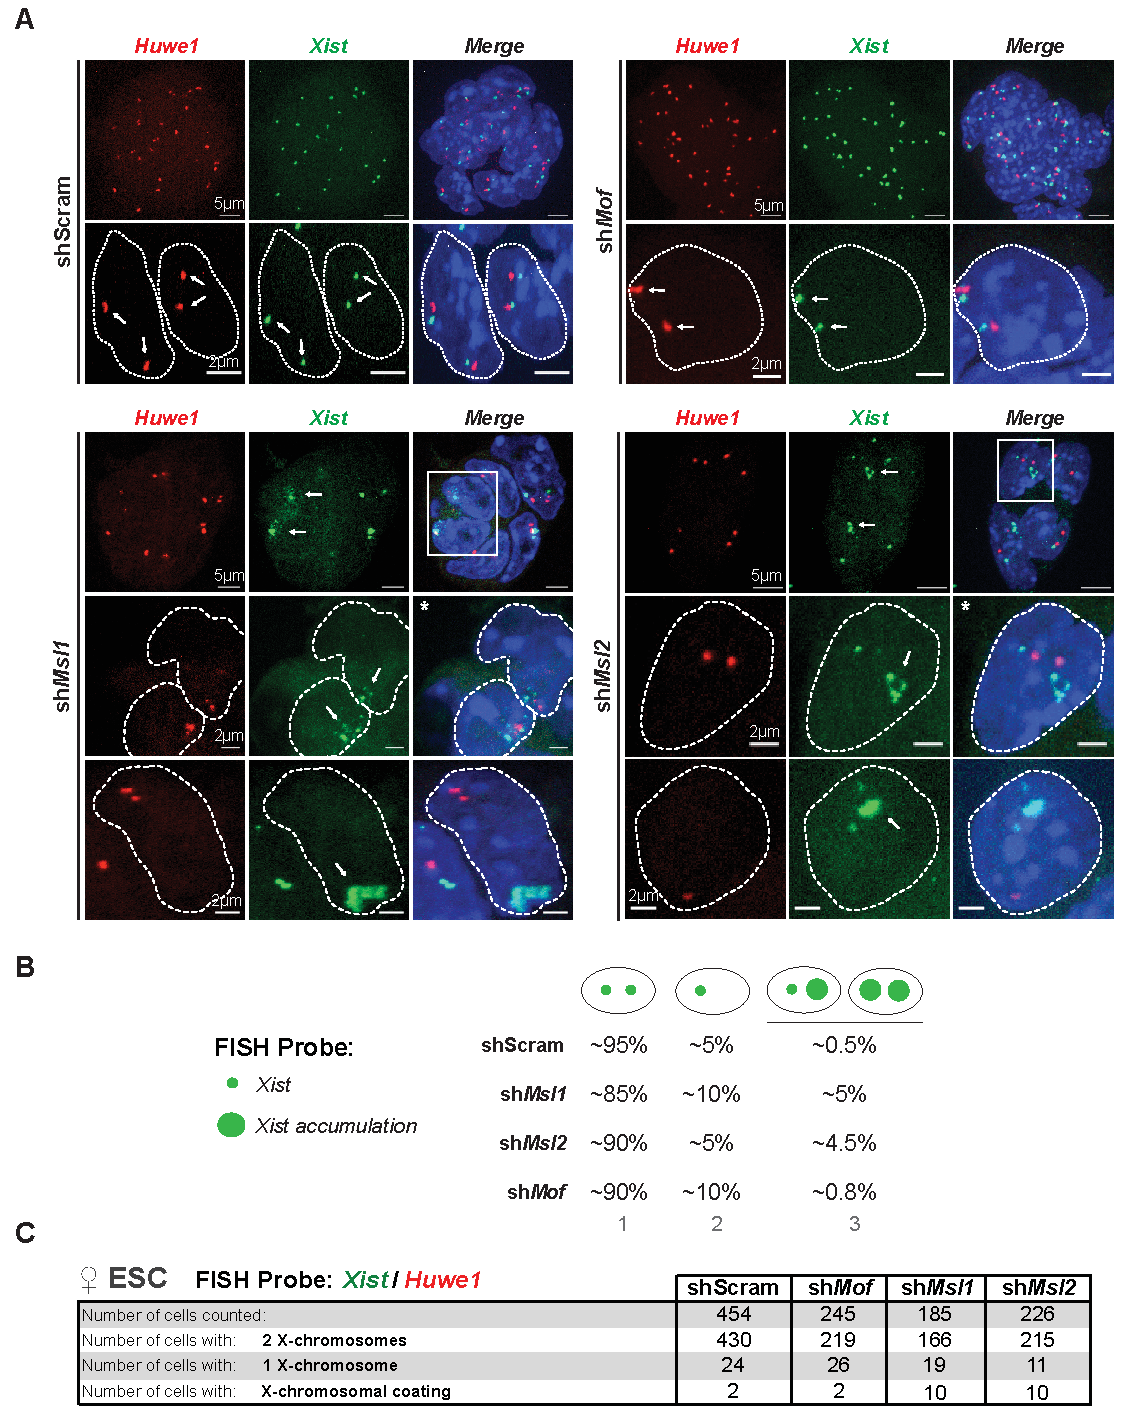
\includegraphics[width=.85\textwidth]{Figures/Appendix/Figure7_supplemental_figure1_scissored.pdf}

\textbf{Figure 7—figure supplement 1: Depletion of MSL1 and MSL2 leads to occasional accumulation and spreading of Xist in undifferentiated ESCs.}

(A) RNA-FISH for \textit{Huwe1} RNA (red) and \textit{Xist} RNA (green) in shScrambled- (top left) and sh\textit{Mof}- (top right), sh\textit{Msl1}- (bottom left) and sh\textit{Msl2}-treated (bottom right) female ESCs. Shown here are additional examples of RNA-FISH for multicellular colonies and individual cells exhibiting \textit{Xist}-mediated coating (see Figure 7A). White boxes indicate cells enlarged in Figure 7A. White arrows denote \textit{Huwe1} and \textit{Xist} foci. Dashed lines indicate nuclei borders. For all experiments, nuclei were coun\-ter\-stained with DAPI (blue).

(B) Summary of RNA-FISH for \textit{Xist} and \textit{Huwe1}. The number of green dots indicates the number of X chromosomes within the cell while the larger dot indicates \textit{Xist} accumulation. Cells were classified into three phenotypic groups with cells showing sharp, localized \textit{Xist} signals (once or twice) or \textit{Xist} ``clouds''. The percentages indicate how many cells per population showed the respective phenotype.

(C) Corresponding to Figure 7A. Summary of the total cell counts from \textit{Xist} and \textit{Huwe1} RNA-FISH in indicated knockdowns.
\newpage
%%%%%%%%%%%%%%%%%%%%%%%%%%
% 7-2
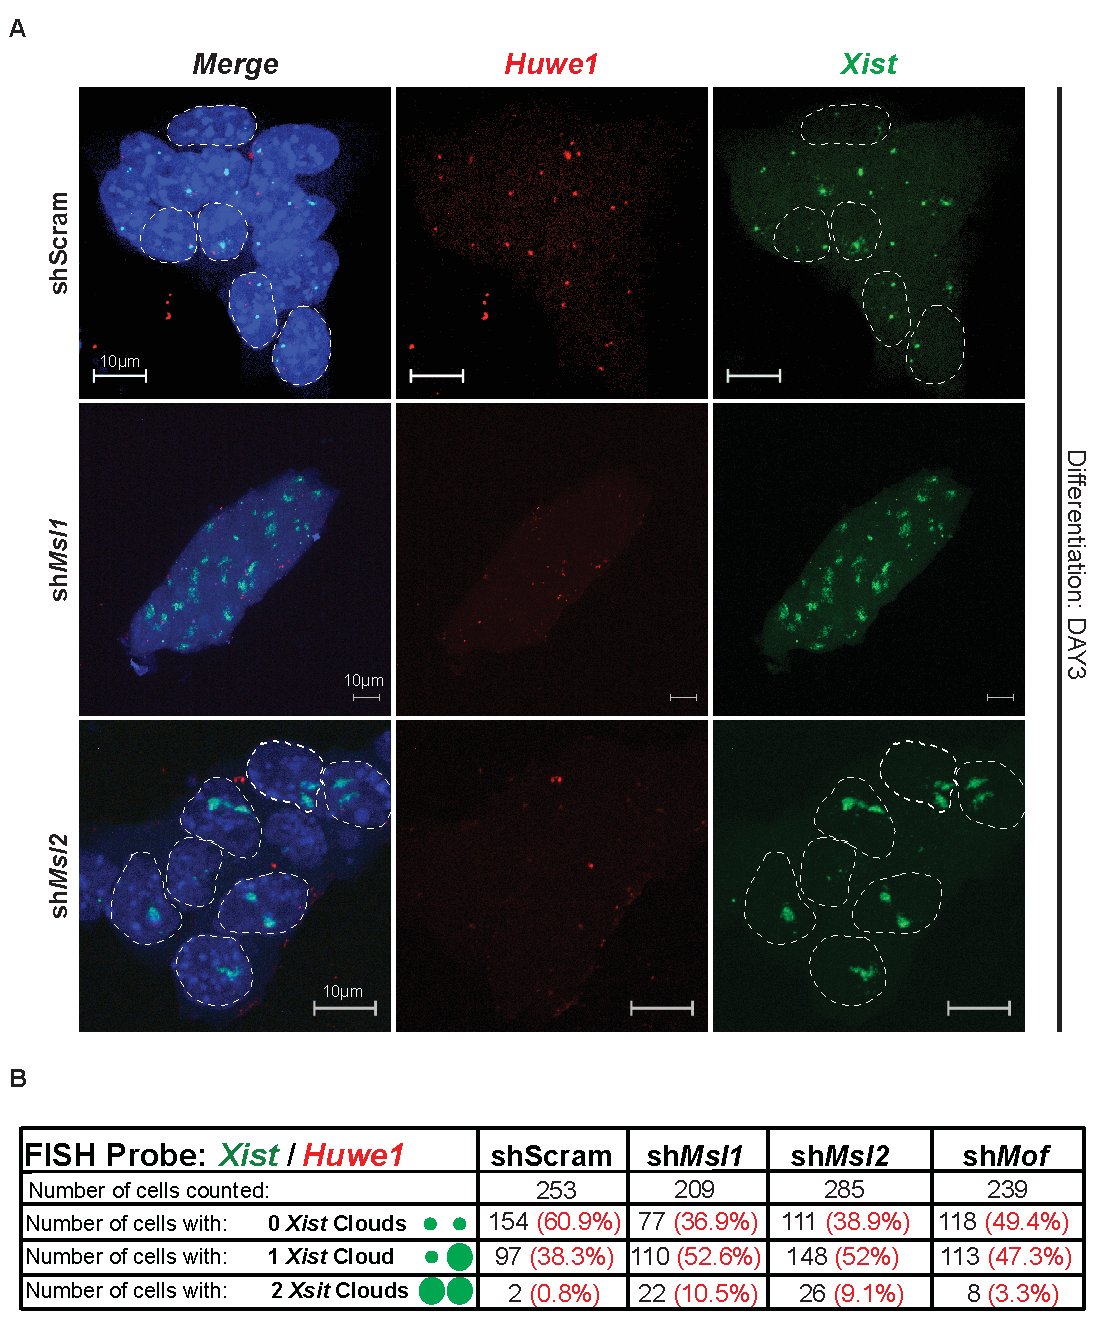
\includegraphics[width=\textwidth]{Figures/Appendix/Figure7_supplemental_figure2_scissored.pdf}

\textbf{Figure 7—figure supplement 2: Depletion of MSL1 and MSL2 lead to enhanced Xist accumulation in differentiating ESCs.}

(A) RNA-FISH for \textit{Huwe1} RNA (red) and \textit{Xist} RNA (green) in shScrambled-, sh\textit{Msl1}- and sh\textit{Msl2}-treated differentiating (DAY3) female ESCs. Shown here are additional examples of RNA-FISH for multicellular colonies (see Figure 7C). Dashed lines indicate nuclei borders. For all experiments, nuclei were coun\-ter\-stained with DAPI (blue).

(B) Corresponding to Figure 7C-E. Summary of the total cell counts from \textit{Xist} RNA-FISH in indicated knockdowns. Percentage of cells with respective phenotype indicated in red.

%===============================
\end{singlespacing}
\end{sffamily}
\end{footnotesize}
\clearpage
%===================================================
%%%%%%%%%%%%%%%%%%%%%%%% DEEPTOOLS
\section{deepTools: a flexible platform for NGS analysis}
\label{SuppPub_deepTools}

\begin{center}
\noindent\overbox[c]{Ramírez,\:F.*, \textbf{D{\"u}ndar,\:F.}*, Diehl,\:S., Gr{\"u}ning,\:B.\:A., Manke,\:T. (2014).\\
Nucleic Acids Research. doi:10.1093/nar/gku365 \\
*shared authorship}
\end{center}

I contributed to the development and debugging of the software tools (which were programmed to the largest extent by Fidel Ramírez).

I designed and generated the entire content of the deepTools documentation and help pages (\url{https://github.com/fidelram/deepTools/wiki}) which are still maintained by me.

I initiated the set-up of the public deepTools Galaxy instance \url{http://deeptools.ie-freiburg.mpg.de/} which was carried out by Sarah Diehl and generated all Galaxy Workflows, information pages (except the video tutorial), and histories.

I contributed to the main figure and devised, wrote, and revised the manuscript together with Fidel Ramírez and Thomas Manke. I generated the supplemental PDF version of the online deepTools documentation that is provided together with the manuscript.

\fancyhead[RO,LE]{Appendix: \emph{Ramírez, D{\"u}ndar et al. (2014), Nucleic Acids Research.}} 
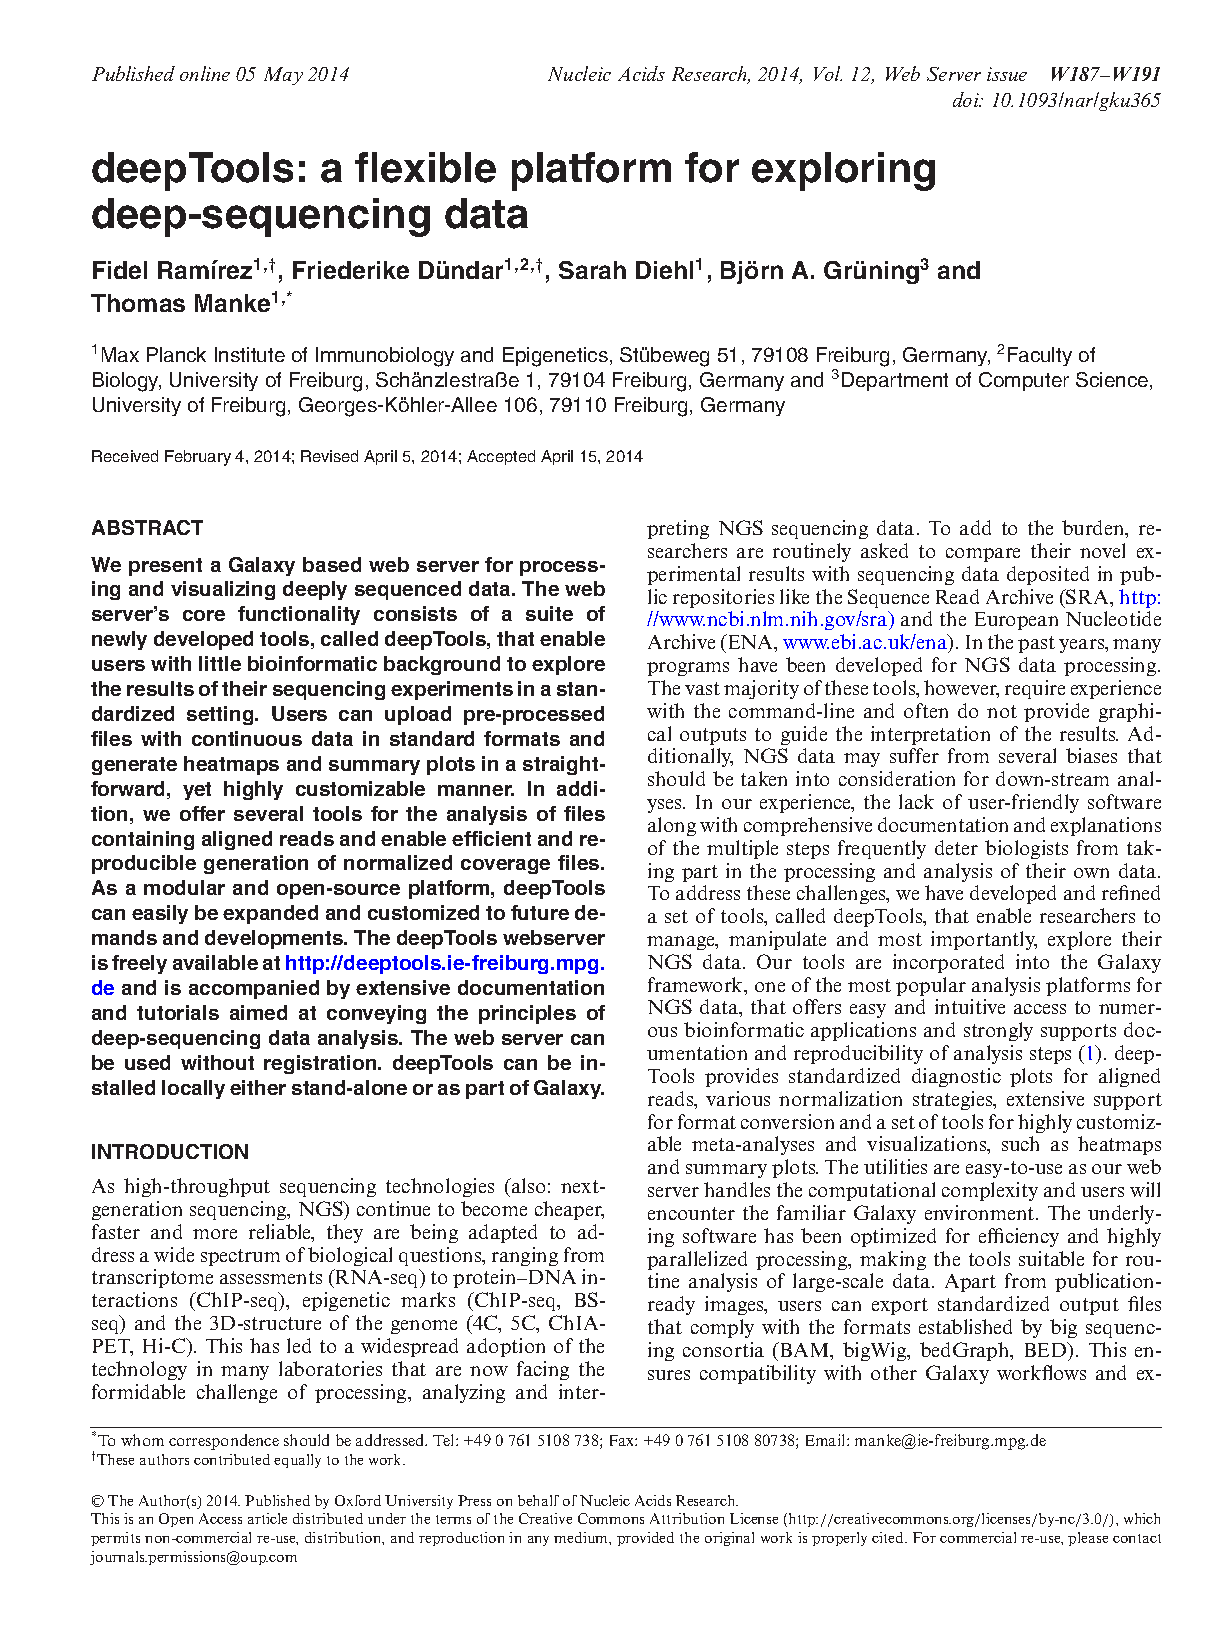
\includepdf[scale=0.9,pages=-,pagecommand={},offset=0.3cm 0cm]{Figures/Appendix/RamirezDundar2014_scissored.pdf}


\subsection{Supplemental Material}
\fancyhead[RO,LE]{Appendix: Supplement to \emph{Ramírez, D{\"u}ndar et al. (2014), Nucleic Acids Research.}} 

\begin{figure}[!h]
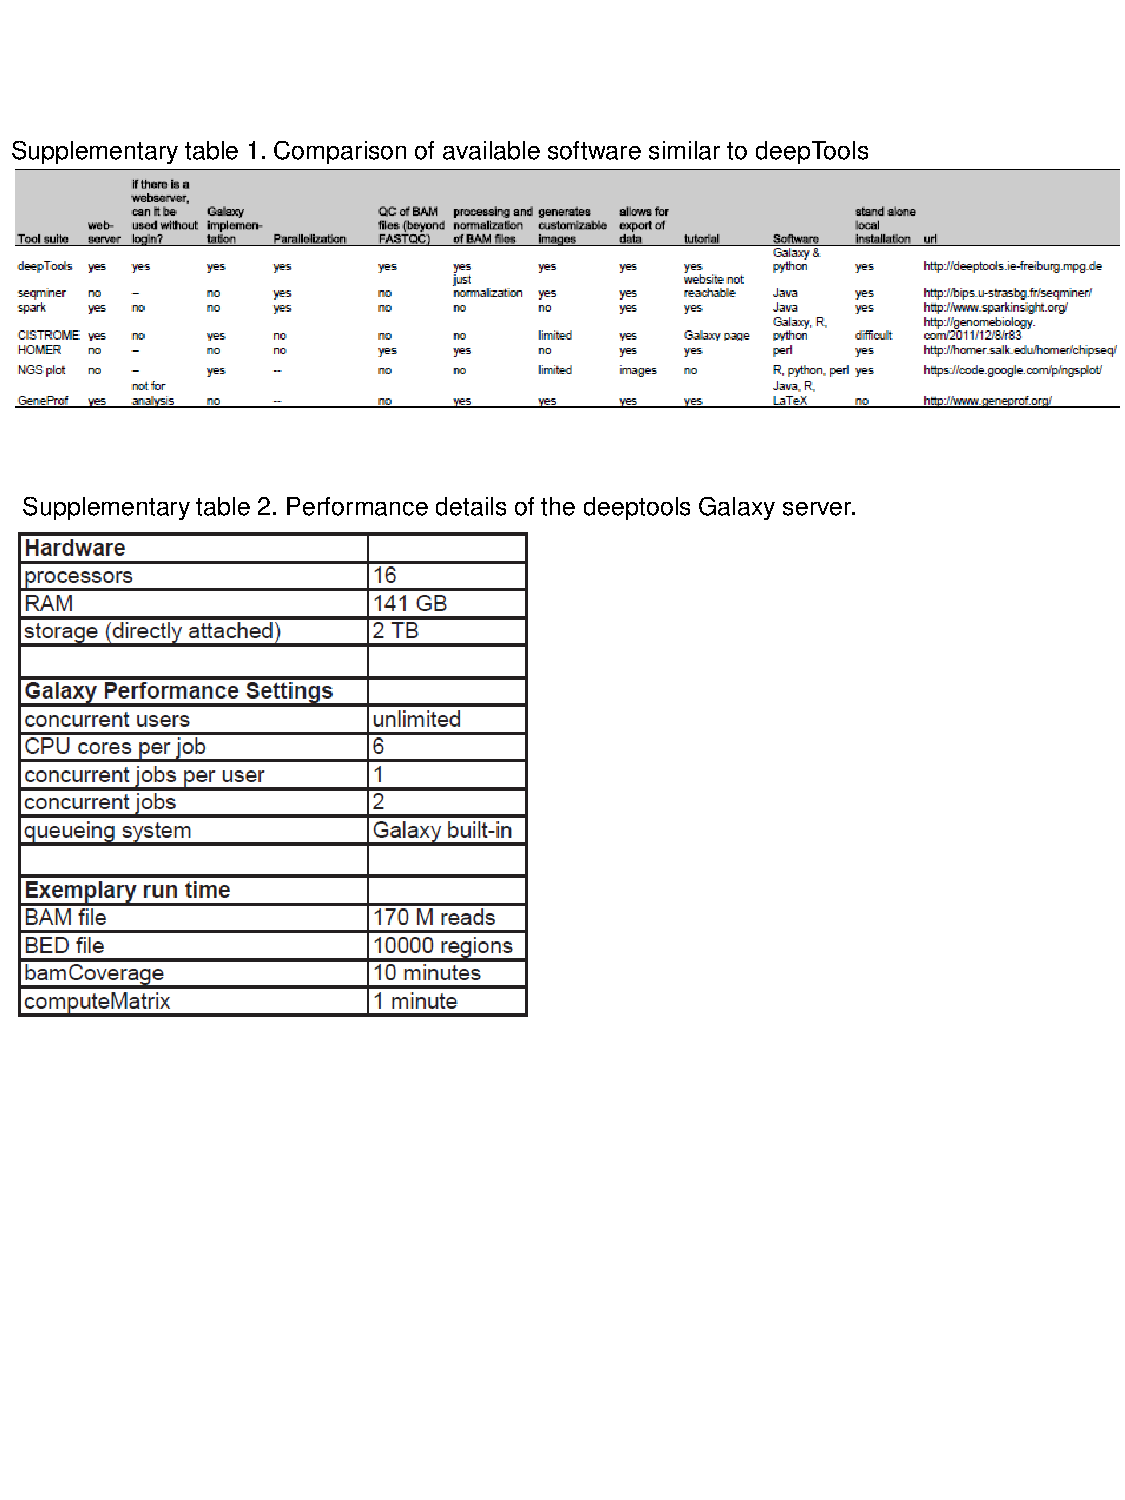
\includegraphics[width=1\textwidth]{Figures/Appendix/RamirezDundar2014_supplementTables.pdf}
\end{figure}
\newpage

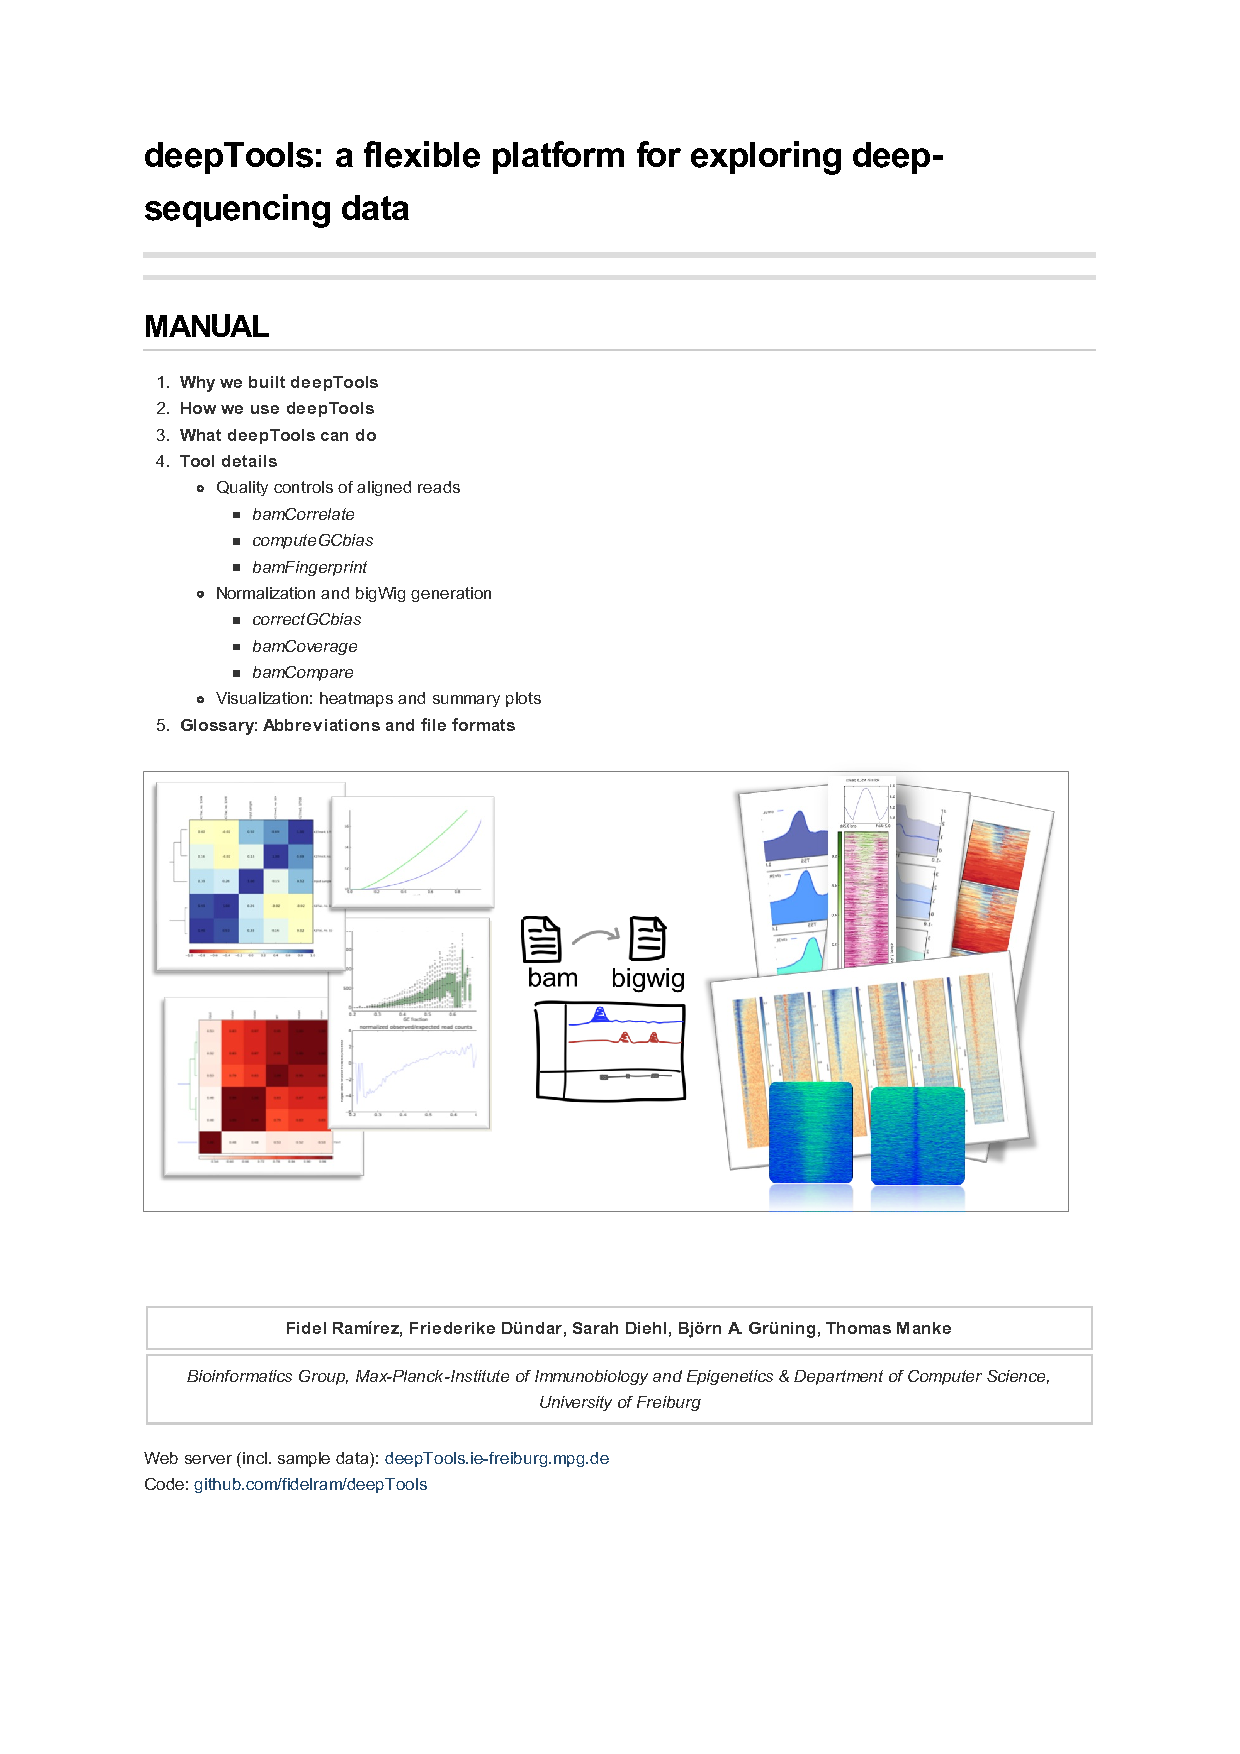
\includepdf[scale=0.9,pages=-,pagecommand={},offset=0.3cm 0cm]{Figures/Appendix/RamirezDundar2014_supplementManual.pdf}

%%%%%%%%%%%%%%%%%%%%%%%% MSL1 at promoters

\fancyhead[RO,LE]{} % header on each page
\section{A regulatory feedback loop between MSL1 and CDK7 controls RNA polymerase II
Serine 5 phosphorylation}
\label{SuppPub_MSL1} 

\begin{center}
\noindent\overbox[c]{
Chlamydas,\:S., Holz,\:H., Pelechano,\:V., Chelmicki,\:T., Georgiev,\:P.,\\
\textbf{D{\"u}ndar,\:F.}, Dasmeh,\:P., Mittler,\:G., Tavares Cadete,\:F., Ramírez,\:F.,\\
Conrad,\:T., Wei,\:W., Raja,\:S., Manke,\:T., Luscombe,\:N.\:M., Steinmetz,\:L.\:M.,\\ Akhtar,\:A. \textit{Submitted for review.}}
\end{center}

I generated Figure 1A and Figure S1C-E using data processed by Fidel Ramírez (\textit{D.~melanogaster}) and myself (\textit{D.~virilis, M.~musculus}) and contributed to the revision of the manuscript.

\textbf{Abstract:}

Proper gene expression requires the coordinated interplay between transcriptional co-activators, transcription factors and the general transcription machinery. We find that MSL1, a component of the \textit{Drosophila} dosage compensation complex, functions as a transcriptional co-activator with CDK7, a subunit of the Cdk-activating kinase (CAK) complex, which phosphorylates Ser5 of the carboxy-terminal domain of RNA polymerase II. The MSL1/CDK7 regulatory feedback loop is evolutionarily conserved and regulates both autosomal and X-linked target gene expression. MSL1 promotes the efficient recruitment and catalytic activity of CAK at core promoters. CDK7-
mediated phosphorylation of MSL1 is essential for its proper targeting to specific autosomal sites and for X chromosome-enrichment of the entire MSL complex in male flies. In addition, MSL1 is required for proper mRNA 5’ capping, bridging transcription with posttranscriptional regulatory events. Thus, the MSL1/CDK7 feedback loop promotes robust target gene expression genome-wide and is distinctly important for dosage compensation in \textit{Drosophila}.

% Appendix A

\chapter{Supplemental Information} % Main appendix title
\label{SuppInfo} % For referencing this appendix elsewhere, use \ref{AppendixA}
%\lhead{Supplemental Information} % This is for the header on each page - perhaps a shortened title
\fancyhead[RO,LE]{Appendix: Supplemental Information}
\fancyfoot{}
\fancyfoot[C]{\thepage}

%
%%%%%%%%%%%%%%%%%%%%%%%%%%%%%
\section{Supplemental material related to the MSL and NSL complexes}
%
\begin{figure}[h!]
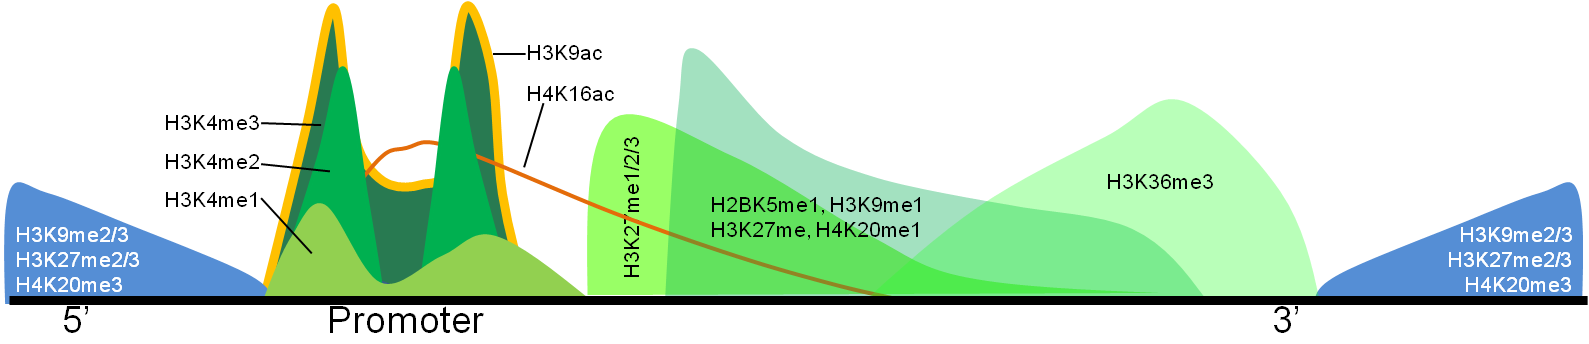
\includegraphics[width=1\textwidth]{Figures/histoneMarkDistribution.png}
\begin{footnotesize}
\setlength{\abovecaptionskip}{0ex}
\caption[Distribution of histone marks along an active gene.]{\textsf{Schematic patterns of selected histone marks along an active gene. Histone modifications associated with active transcription are shown in green (methylation) and orange (acetylation), repressive histone marks are shown in blue. Active promoters are strongly labelled with H3K9ac and H3K4me3, surrounded by H3K4me2/1. Inactive genes are typically covered with H3K9me2/3, H4K20me3 and H3K27me3 that also peaks around the silenced promoters. The image is based on \citep{Barth2010}. Note that the signal of H4K16ac for dosage compensated genes in \textit{Drosophila} inreases towards the 3'-end.}}
\label{fig:histoneDistribution}
\end{footnotesize}
\end{figure}
%\subsection{Protein names}
%\begin{minipage}{\textwidth} % to avoid pagebreaks despite longtable environment
\begin{singlespacing}
\begin{small}
\setlength{\extrarowheight}{2pt}
%\vspace*{-2em}
\begin{longtable}[l]{>{\textsf\bgroup}p{5.5cm}<{\egroup} >{\textsf\bgroup}p{8.5cm}<{\egroup}} % defining the columns - these must match the widths defined for the mini pages down below!
\caption[Protein names of MSL- and NSL complex members in \textit{D.~melanogaster} and mammals.]{\textsf{Protein names of MSL- and NSL complex members in \textit{D.~melanogaster}, mouse and humans. Bold font indicates the name that I used throughout most of the manuscript unless noted otherwise. MSL = male-specific lethal, NSL = non-specific lethal}} \\ % the \\ is important!
%%%%%%%%%%%%%%%
% table title
\textbf{\textit{Drosophila}} & \textbf{Mammals}
\tabularnewline \hline
\endfirsthead 
%
\multicolumn{2}{c}%
{\tablename\ \thetable\ -- \textit{Continued from previous page}} \\[1ex]
\textbf{\textit{Drosophila}} & \textbf{Mammals}
\tabularnewline \toprule %\tabularnewline [1ex]
\endhead % Line(s) to appear at top of every page (except first)
\multicolumn{2}{r}{\textit{Continued on next page}} \\
\endfoot % Last line(s) to appear at the bottom of every page (except last)
\endlastfoot
%-----------------------
%%%%%%%%%%%%%%%
 \textbf{MOF} (males absent on first) & MYST1, hMOF, KAT8 (lysine acetyl transferase 8)
\tabularnewline \midrule
%--------------------------
\textbf{MSL1} & hMSL1
\tabularnewline \midrule
%--------------------------
\textbf{MSL2} & hMSL2, Msl2l1, Rnf184 (ring finger~184)
\tabularnewline \midrule
%--------------------------
\textbf{MSL3} & hMSL3, Msl31
\tabularnewline \midrule
%--------------------------
\textbf{MLE} (maleless) & DHX9 (aspartic-acid-glutamine-alanine-histidin (DEAH) box helicase~9)
\tabularnewline \midrule
%--------------------------
\textbf{NSL1}, waharan & hMSL1v1, Kansl1 (KAT8 regulatory NSL complex subunit~1)
\tabularnewline \midrule
%--------------------------
\textbf{NSL2}, dgt1~(dimmed gamma tubulin~1) & Kansl2 (KAT8 regulatory NSL complex subunit~2)
\tabularnewline \midrule
%--------------------------
\textbf{NSL3}, Rcd1~(reduction in cen\-tro\-somin dots) & Kansl3 (KAT8 regulatory NSL complex subunit~3)
\tabularnewline \midrule
%--------------------------
\textbf{MBD-R2} (methyl-binding domain protein) & PHF20~(plant homeo domain~(PHD) finger protein~20), GLEA2~(glioma-expressed antigen~2)
\tabularnewline \midrule
%--------------------------
\textbf{MCRS2}, dMCRS1, p78, Rcd5~(reduction in cen\-tro\-somin dots) & p78, MSP58~(microspherule protein~58)
\tabularnewline \midrule
%--------------------------
\textbf{WDS} (will die slowly) & WDR5 (tryptophan-aspartic acid~(WD) repeat domain~5)
%--------------------------
\tabularnewline \bottomrule
%-----------------------------
\label{tab:Names}
\end{longtable}
\end{small}
\end{singlespacing}
%\end{minipage}
%
%\subsection{Cancer-related observations}
\vspace*{-4em}
\begin{minipage}{\textwidth} % to avoid pagebreaks despite longtable environment
\begin{singlespacing}
\begin{small}
\setlength{\extrarowheight}{2pt}
\begin{longtable}[l]{>{\textsf\bgroup}p{2cm}<{\egroup} >{\textsf\bgroup}p{12.5cm}<{\egroup}} % defining the columns - these must match the widths defined for the mini pages down below!
\caption[Association of MSL and NSL complex members with human cancers.]{\textsf{Association of MSL and NSL complex members with human cancers. Note that I used the mammalian protein names, see \tref{tab:Names} for synonyms and \textit{Drosophila} names.}} \\ % the \\ is important!
%%%%%%%%%%%%%%%
% table title
\textbf{Protein} & \textbf{Observation}
\tabularnewline
%-----------------------
\toprule
 MYST1 & \begin{minipage}{12.5cm}
				\begin{itemize}[noitemsep,leftmargin=*]
					\item downregulated in colorectal, gastric, ovarian, hepatocellular, breast cancer and renal cell carcinoma \citep{Pfister2008,Giampieri2013,Liu2013,Wang2013,Cao2014,Zhang2014a}, loss of H4K16ac is a hallmark of numerous cancers \citep{Fraga2005}
					\item upregulated in human non-small-cell lung cancer \citep{Chen2014}
					\end{itemize}
				\end{minipage}
\tabularnewline \midrule
%--------------------------
MSL1 & single nucleotide polymorphism in \textit{MSL1} is associated with decreased risk of invasive serous ovarian cancer \citep{Peedicayil2010} 
\tabularnewline \midrule
%--------------------------
MSL3 & might enhance the proliferation of hematopoetic cells in acute myeloid leukemia \citep{Sinenko2010}
\tabularnewline \midrule
%--------------------------
PHF20 & \begin{minipage}{12.5cm}
\begin{itemize}[noitemsep, leftmargin=*]
\item auto-antibodies against PHF20 are positively correlated with the survival rate of neuroblastoma patients \citep{Fischer2001,Pallasch2005}
\item high expression in non-small-cell lung cancer \citep{Taniwaki2006}, genetic alteration of \textit{PHF20} are associated with its progression \citep{Bankovic2010}
\end{itemize}
\end{minipage}
\tabularnewline \midrule
%--------------------------
MCRS1 & \begin{minipage}{12.5cm}
					\begin{itemize}[noitemsep, leftmargin=*]
							\item oncogene with the potential for malignant cell transformation \cite{Okumura2005a,Hsu2012}
							\item upregulated in all investigated cancer types \citep{Shi2012,Wu2012,Lin2013,Zhong2013}
					\end{itemize}
				\end{minipage}
\tabularnewline \midrule
%--------------------------
WDR5 & implicated in the establishment and progression of leukemia due to its interaction with the methyl transferase MLL (mixed-lineage leukemia; reviewed by \citet{Wu2011a})
%--------------------------
\tabularnewline \bottomrule
%-----------------------------
\label{tab:cancer}
\end{longtable}
\end{small}
\end{singlespacing}
\end{minipage}

%
%\subsection{Enzymes within the complexes}
\begin{minipage}{\textwidth} % to avoid pagebreaks despite longtable environment
\begin{singlespacing}
\begin{small}
\setlength{\extrarowheight}{1.5pt}
\vspace*{-2em}
\begin{longtable}[l]{>{\textsf\bgroup}p{2cm}<{\egroup}>{\textsf\bgroup}p{2cm}<{\egroup} >{\textsf\bgroup}p{4cm}<{\egroup}} % defining the columns - these must match the widths defined for the mini pages down below!
\caption[Enzymes within the MSL and NSL complexes.]{\textsf{Enzymes within the MSL and NSL complexes.}} \\ % the \\ is important!
%%%%%%%%%%%%%%%
% table title
\textbf{Complex} & \textbf{Protein} & \textbf{Function}
\tabularnewline
%-----------------------
\toprule
MSL, NSL & MOF & histone acetyl transferase
\tabularnewline \midrule
\multirow{2}{*}{MSL} 	& MSL2 & E3 ubiquitin ligase \\
											& MLE & DNA and RNA helicase
\tabularnewline \midrule
NSL & NSL3 & putative hydrolase function 
\tabularnewline \bottomrule
%-----------------------------
\label{tab:enzymes}
\end{longtable}
\end{small}
\end{singlespacing}
\end{minipage}

%
%---------------------------------
%%% Figure NSL targets
\begin{figure}[tb]
	\begin{minipage}[c]{0.50\textwidth}
		\includegraphics[width=\textwidth]{Figures/NSLtargetgenes_scissored.pdf}
	\end{minipage} \hfill
	%%%%%%%%%%
	\begin{minipage}[c]{0.4\textwidth}
		\begin{footnotesize}
			\caption[ChIP-seq signals of MSL complex members for NSL targets and NSL-non-bound genes in \textit{Drosophila}.]{\textsf{ChIP-seq signals of MSL complex members for NSL targets and NSL-non-bound genes in \textit{Drosophila}. All images were generated with \texttt{computeMatrix} and \texttt{heatmapper} from the deepTools suite \citep{Ramirez2014} using the scale-regions mode to scale gene bodies to 2~kb. See \tref{tab:ChIPseqSamplesDmel} and \ref{tab:Becker} for details about the ChIP-seq data sets.
\textbf{A)} There is no difference in the ChIP-seq signals of MOF, H4K16ac and MSL1 from female larva for autosomal (chromosome 2L, chr2L) and X-linked (chrX) genes, but there are almost exclusively strong enrichments for NSL targets.
\textbf{B)} In males, the signals of the MSL complex are visibly stronger for X-linked NSL targets, but only MSL3 and H4K16ac show significant enrichments for non-NSL-bound genes.}}
			\label{fig:NSLtargetgenes}
		\end{footnotesize}
	\end{minipage}
\end{figure}

\clearpage

%---------------------------------

%\vspace*{-2em}
%\begin{landscape}
\begin{minipage}{\textwidth}
\begin{singlespacing}
\begin{small}
\begin{sffamily}
\begin{longtable}[l]{>{\textsf\bgroup}p{3.8cm}<{\egroup} >{\raggedright\arraybackslash}p{2.7cm} >{\textsf\bgroup}p{7cm}<{\egroup}}
\caption[MOF-associated proteins in transcription activation.]{\textsf{MOF-associated proteins in transcription activation. Related to \fref{fig:functions}.}} \\ % the \\ is important! see http://tex.stackexchange.com/questions/103698/extra-alignment-tab-with-longtable
%%%%%%%%%%%%%%%
% table title
\textbf{Proteins} & \textbf{Function} & \textbf{Biological effect}
\tabularnewline \toprule
%\endfirsthead % indicates that the lines above appear as head of the table on the first page
%\multicolumn{3}{c}%
%{\tablename\ \thetable\ -- \textit{Continued from previous page}} \\ [2ex]
%\textbf{Proteins} & \textbf{Function} & \textbf{Biological effect}
%\tabularnewline \toprule \tabularnewline [1ex]
%\endhead % Line(s) to appear at top of every page (except first)
%\multicolumn{3}{r}{\textit{Continued on next page}} \\
%\endfoot % Last line(s) to appear at the bottom of every page (except last)
%\endlastfoot
%%%%%%%%%%%%%%%%%%%
%%% let's start the table content; each column (often) gets its own minipage which enables itemized lists etc.
%%%%%%%%%%%%%%%%%%%
%% first row
%-----------------------
%\\ \multicolumn{3}{c}{\textbf{\textsf{Gene expression}}}
%\\ [2ex] \hline \\ [1ex]
%------------------
\begin{minipage}[c]{3.8cm}
				\vskip 2pt
					MOF within the\\MSL complex \\
				(MSL1, MSL2,\\MSL3, MLE (roX))
				\vskip 2pt
			\end{minipage}
			& \begin{minipage}[c]{2.7cm}
					\raggedright acetylation of H4K16ac \citep{Akhtar2000,Taipale2005,Li2009} \\
			\end{minipage}
					& \begin{minipage}[c]{7cm}
					\vskip 2pt
									\begin{itemize}[noitemsep, leftmargin=*]
										\item opening of chromatin (reviewed by \citet{Preez2013})
										\item dosage compensation in male \textit{D.~melano\-gaster} that entails the upregulation of the entire X chromosome \citep{Conrad2011}
									\end{itemize}				
									\vskip 2pt
							\end{minipage}
%\\ [2ex] \hline \\ [1ex]
\tabularnewline \midrule
%-----------------------
\begin{minipage}[c]{3.8cm}
\vskip 2pt
					MOF within the\\NSL complex \\
				(NSL1, NSL2, NSL3,\\MCRS2, MBD-R2, WDS)
				\vskip 4pt
			\end{minipage}
			& \begin{minipage}[c]{2.7cm}
							\raggedright acetylation of H4K16 \citep{Li2009}, H4K5, H4K8 \citep{Cai2010}
			\end{minipage}
					& \begin{minipage}[c]{7cm} % 3rd column
									\begin{itemize}[noitemsep, leftmargin=*]
										\item opening of chromatin \citep{Preez2013}
										\item housekeeping gene regulation \citep{Feller2012, Lam2012}
									\end{itemize}				
							\end{minipage}
%\\ [2ex] \hline \\ [1ex]
\tabularnewline \midrule
%-----------------------
\begin{minipage}[c]{3.8cm}
					MSL2
			\end{minipage}
			& \begin{minipage}[c]{2.7cm}
			\vskip 2pt
					\raggedright ubiquitylation of H2BK34 \citep{Wu2011}
					\vskip 4pt
			\end{minipage}
					& \begin{minipage}[c]{7cm} % 3rd column
					\vskip 2pt
							implicated to stimulate methylation of H3K4 \citep{Wu2011} and transcription elongation \citep{Wu2014}
							\vskip 4pt
							\end{minipage}
\tabularnewline \midrule
%\\ [2ex] \hline \\ [1ex]
%-----------------------
\begin{minipage}[c]{3.8cm}
\vskip 2pt
					MCRS2
					\vskip 4pt
\end{minipage}
			& \begin{minipage}[c]{2.7cm}
			\vskip 2pt
					interaction partner
					\vskip 4pt
			\end{minipage}
					& \begin{minipage}[c]{7cm} % 3rd column
					\vskip 2pt
							facilitates Pol~II recruitment to target genes \citep{Andersen2010}
							\vskip 4pt
						\end{minipage}
%\\ [2ex] \hline\pagebreak
%-----------------------
%\multicolumn{3}{c}{\textbf{\textsf{Cell-cycle-associated processes}}}
%\\ [2ex] \hline \\ [1ex]
%-----------------------
%%%%%%%%%%%%%%%%%%%%%%%%%%
\tabularnewline \bottomrule
\label{tab:functions1}
\end{longtable}
\end{sffamily}
\end{small}
\end{singlespacing}
\end{minipage}

%%\vspace*{-2em}
\begin{minipage}{\textwidth}
\begin{singlespacing}
\begin{small}
\begin{sffamily}
\begin{longtable}[l]{>{\raggedright\arraybackslash}p{3cm} >{\raggedright\arraybackslash}p{11cm}}
\caption[MOF-associated proteins in cell-cycle-related processes.]{\textsf{MOF-associated proteins in cell-cycle-related processes. Related to \fref{fig:functions}}} \\ % the \\ is important! 
%%%%%%%%%%%%%%%
% table title
\textbf{Biological process} & \textbf{Observation} 
\tabularnewline \toprule
%==========================
\begin{minipage}[c]{3cm}
					G2/M checkpoint
			\end{minipage}
					& \begin{minipage}[c]{11cm} % 3rd column
					\vskip 4pt
							NSL1, NSL2, NSL3, MCRS2, MBD-R2 and WDS were identified as essential factors for G2/M checkpoint progression following DNA damage in \textit{D.~melano\-gaster} \citep{Kondo2011}
							\vskip 4pt
							\end{minipage}
\tabularnewline \midrule
%\\ [2ex] \hline \\ [1ex]
%-----------------------
\begin{minipage}[c]{3cm}
					mitotic spindle
			\end{minipage}
					& \begin{minipage}[c]{11cm} % 3rd column
					\vskip 4pt
							\begin{itemize}[noitemsep, leftmargin=*]
							\item NSL2 is needed for mitotic spindle assembly \citep{Goshima2007}
							\item MCRS1 stabilizes the mitotic spindle \citep{Meunier2011}
							\item WDS was identified in a screen for microtubule-associated proteins \cite{Hughes2008}
							\end{itemize}
							\vskip 2pt
							\end{minipage}
\tabularnewline \midrule
%------------------------
\begin{minipage}[c]{3cm}
					apoptosis
			\end{minipage}
					& \begin{minipage}[c]{11cm} % 3rd column
					\vskip 4pt
							\begin{itemize}[noitemsep, leftmargin=*]
							\item ubiquitylation of p53 by MSL2 leads to accumulation of p53 in the cytoplasm \citep{Kruse2009} which is necessary for apoptosis \cite{Muscolini2011}
							\item MOF acetylates p53 in the presence of NSL1 \citep{Li2009} which is necessary for apoptosis induction in cells with DNA damages \citep{Sykes2006, Sykes2009}
							\item human MBD-R2 (PHF20) stimulates expression of p53 and prevents its degradation via a direct interaction with methylated p53 \citep{Park2009, Cui2012}
							\end{itemize}
							\vskip 2pt
							\end{minipage}
\tabularnewline \midrule
%------------------------
\begin{minipage}[c]{3cm}
					DNA repair
			\end{minipage}
					& \begin{minipage}[c]{11cm} % 3rd column
					\vskip 4pt
							\begin{itemize}[noitemsep, leftmargin=*]
								\item MOF is generally required for repair of DNA double strand breaks and recruitment of 53BP1 and BRCA \cite{Sharma2010, Li2010}; its phosphorylated form is particularly important for biasing the cells towards homologous repair during S~phase by displacing 53BP1 from the site of the DNA damage \citep{Gupta2014}
								\item human MSL2 ubiquitylates 53BP1 \citep{Lai2013}
								\item human MSL1 interacts with 53BP1 that positively stimulates DNA damage repair \citep{Gironella2009}
							\end{itemize}
							\vskip 2pt
							\end{minipage}
%%%%%%%%%%%%%%%%%%%%%%%%%%
\tabularnewline \bottomrule
\label{tab:functions2}
\end{longtable}
\end{sffamily}
\end{small}
\end{singlespacing}
\end{minipage}
%
%%%%%%%%%%%%%%%%%%%%%%%%%%%%%%%%%
\section{Supplemental bioinformatics-related tables}
%
%\subsection{Bioinformatic tools and software}
%\begin{landscape}
\begin{singlespacing}
\begin{small}
%\setlength{\extrarowheight}{15pt} % this doesn't work to control the vertical space
\vspace*{-1em}
\begin{longtable}{>{\textsf\bgroup\raggedleft\arraybackslash}p{2.7cm}<{\egroup} >{\textsf\bgroup}p{4.5cm}<{\egroup} >{\textsf\bgroup}p{4.2cm}<{\egroup}>{\textsf\bgroup}p{2.3cm}<{\egroup}} % defining the columns - these must match the widths defined for the mini pages down below!
\caption[Bioinformatic tools used for analyses presented here.]{\textsf{Bioinformatic tools used for analyses presented here (alphabetical order; if available, I indicated the versions of the tools that I used). For explanations of the file formats mentioned here, please see the glossary within the supplement of \aref{SuppPub_deepTools}.}} \\ % the \\ is important! see http://tex.stackexchange.com/questions/103698/extra-alignment-tab-with-longtable
%%%%%%%%%%%%%%%
% table title
\textbf{Name} & \textbf{Application} & \textbf{Website} & \textbf{Reference}
\tabularnewline \hline
\endfirsthead % indicates that the lines above appear as head of the table on the first page
\multicolumn{4}{c}%
{\tablename\ \thetable\ -- \textit{Continued from previous page}} \\[1ex]
\textbf{Name} & \textbf{Application} & \textbf{Website} & \textbf{Reference}
\tabularnewline \toprule %\tabularnewline [1ex]
\endhead % Line(s) to appear at top of every page (except first)
\multicolumn{4}{r}{\textit{Continued on next page}} \\
\endfoot % Last line(s) to appear at the bottom of every page (except last)
\endlastfoot
%%%%%%%%%%%%%%%%%%%
%% first row
%-----------------------
\toprule %\\ [4ex]
 \begin{minipage}{2.7cm}
				\textbf{bedtools} \\
					(2.10. to 2.17)
				\end{minipage}
			&	 \begin{minipage}{4.5cm}
				working with genomic intervals, e.g. intersecting two files with different peak regions
			\end{minipage} 
			&  \begin{minipage}{4.2cm}
			\url{http://bedtools.readthedocs.org/en/latest/}
			\end{minipage} 
			&  \begin{minipage}{2.3cm}
					\raggedright \citet{Quinlan2010}
				\end{minipage} 
%\\ [4ex] \hline \\ [1ex]
\tabularnewline \midrule
%---------------------------
 \begin{minipage}{2.7cm}
				\textbf{bowtie} \\
					bowtie-1.0.0\\(Appendix \ref{SuppPub_NSL}),\\
					bowtie2-2.2.2\\(Appendix \ref{SuppPub_MSL}) %\\ [2ex]
			\end{minipage} 
			&  \begin{minipage}{4.5cm}
			alignment of reads to the reference genome
				\end{minipage} 
				&  \begin{minipage}{4.2cm}
				\url{http://bowtie-bio.sourceforge.net/index.shtml}
				\end{minipage} 
				&  \begin{minipage}{2.3cm}
				Langmead and\\
				Salzberg \citep{Langmead2012}
			\end{minipage} 
%\\ [4ex] \hline \\ [1ex]
\tabularnewline \midrule
%-----------------------
 \begin{minipage}{2.7cm}
				\textbf{ChIPEnrich}
			\end{minipage} 
			&  \begin{minipage}{4.5cm}
					gene ontology enrichments for target genes identified by ChIP-seq
			\end{minipage} 
			&  \begin{minipage}{4.2cm}
					\url{http://sartorlab.ccmb.med.umich.edu/chip-enrich}
			\end{minipage} 
			&  \begin{minipage}{2.3cm}
				\citet{Welch2014}
			\end{minipage} 
%\\ [4ex] \hline \\ [1ex]
\tabularnewline \midrule
%-----------------------------
 \begin{minipage}{2.7cm}
		\textbf{DAVID}
\end{minipage} 
			&  \begin{minipage}{4.5cm}
				gene identifier mapping and gene ontology term enrichment analyses
			\end{minipage} 
			&  \begin{minipage}{4.2cm}
				\url{http://david.abcc.ncifcrf.gov/}
			\end{minipage} 
				&  \begin{minipage}{2.3cm}
				\citet{Huang2009}
			\end{minipage} 
%\\ [4ex] \hline \\ [1ex]
\tabularnewline \midrule
%-----------------------------
 \begin{minipage}{2.7cm}
					\textbf{deepTools} \\
					(up to 1.5.7) %\\ [2ex]
			\end{minipage} 
			&  \begin{minipage}{4.5cm}
				quality controls of BAM files, normalizations, coverage file generation, visualizations with heatmaps and summary plots %\\ [2ex]
			\end{minipage} 
			&  \begin{minipage}{4.2cm}
				\url{http://deeptools.github.io/} %\\ [2ex]
			\end{minipage} 
				&  \begin{minipage}{2.3cm}
		\raggedright Ramirez, Dündar et al. \citep{Ramirez2014} %\\ [2ex]
			\end{minipage} 
%\\ [4ex] \hline \\ [1ex]
\tabularnewline \midrule
%-----------------------------
 \begin{minipage}{2.7cm}
					\textbf{DESeq}\\
					(1.10.1)
				\end{minipage} 
			&  \begin{minipage}{4.5cm}
				calculating normalized fold change values for Pol~II ChIP-seq data set \citep{EBIroutine}
			\end{minipage} 	
			&  \begin{minipage}{4.2cm}
				\url{http://www-huber.embl.de/users/anders/DESeq/}
			\end{minipage}
				& 
				\begin{minipage}{2.3cm}
		\citet{Anders2010}
			\end{minipage} 
%\\ [4ex] \hline \\ [1ex]
\tabularnewline \midrule
%---------------------------
 \begin{minipage}{2.7cm}
				\textbf{fastqc}
				\end{minipage}
			&  \begin{minipage}{4.5cm}
				quality control of FASTQ files
			\end{minipage} 
			&  \begin{minipage}{4.2cm}
				\url{http://www.bioinformatics.babraham.ac.uk/projects/fastqc/}
			\end{minipage} 
			&  not available
%\\ [4ex] \hline \\ [1ex]
\tabularnewline \midrule
%-----------------------------
 \begin{minipage}{2.7cm}
				\textbf{Galaxy} %%\\ [2ex]
				\end{minipage} 
			&  \begin{minipage}{4.5cm}
				vast collection of tools for manifold tasks including working with genomic intervals, joining of lists, motif search etc. %\\ [2ex]
			\end{minipage} 
			&  \begin{minipage}{4.2cm}
				in-house installation %%\\ [2ex]
			\end{minipage} 
					&  \begin{minipage}{2.3cm}
		\citet{Goecks2010} %%\\ [2ex]
			\end{minipage} 
%\\ [4ex] \hline \\ [1ex]
\tabularnewline \midrule
%-----------------------------
 \begin{minipage}{2.7cm}
					\textbf{ggplot2}\\
					(0.9.3.1)
			\end{minipage} 
			&  \begin{minipage}{4.5cm}
				R package for highly customizable plots (e.g. boxplots, x-y plots, bar charts etc.)
			\end{minipage} 
			&  \begin{minipage}{4.2cm}
				\url{http://ggplot2.org/}
			\end{minipage} 
			&  \begin{minipage}{2.3cm}
		\citet{ggplot2}
			\end{minipage} 
%\\ [4ex] \hline \\ [1ex]
\tabularnewline \midrule
%-----------------------------
 \begin{minipage}{2.7cm}
					\textbf{GREAT}\\
					(2.0)
				\end{minipage} 
			&  \begin{minipage}{4.5cm}
				web-based tool for target gene prediction
			\end{minipage} 
			&  \begin{minipage}{4.2cm}
				\url{http://bejerano.stanford.edu/great/public/html/}
			\end{minipage} 
				&  \begin{minipage}{2.3cm}
		\citet{McLean2010}
			\end{minipage} 
%\\ [4ex] \hline \\ [1ex]
\tabularnewline \midrule
%----------------------------
 \begin{minipage}{2.7cm}
					\textbf{Integrative\\Genomics\\Viewer}\\
					(up to 2.3.32) %\\ [2ex]
			\end{minipage} 
			& 	\begin{minipage}{4.5cm}
				genome browser for visualization of BAM, BED, bigWig and bedGraph files %\\ [2ex]
			\end{minipage} 
			&  \begin{minipage}{4.2cm}
				\url{http://www.broadinstitute.org/igv/} %\\ [2ex]
			\end{minipage} 
				&  \begin{minipage}{2.3cm}
		\citet{Thorvaldsdottir2013} %\\ [2ex]
			\end{minipage} 
%\\ [4ex] \hline \\ [1ex]
\tabularnewline \midrule
%-----------------------------
 \begin{minipage}{2.7cm}
					\textbf{liftover}\\
					(2013)
			\end{minipage} 
			&  \begin{minipage}{4.5cm}
				conversion of sequence coordinates from mm8 assembly to mm9
			\end{minipage} 
			&  \begin{minipage}{4.2cm}
				\url{https://genome.ucsc.edu/cgi-bin/hgLiftOver}
			\end{minipage} 
				&  not available
%\\ [4ex] \hline \\ [1ex]
\tabularnewline \midrule
%-----------------------------
 \begin{minipage}{2.7cm}
				\textbf{MACS}\\
					(1.4.2)
				\end{minipage}
			&	 \begin{minipage}{4.5cm}
				identification of significantly enriched ChIP-seq regions
			\end{minipage} 
			&  \begin{minipage}{4.2cm}
				\url{http://liulab.dfci.harvard.edu/MACS/}
			\end{minipage} 
				&  \begin{minipage}{2.3cm}
		\citet{Zhang2008}
			\end{minipage} 
%\\ [4ex] \hline \\ [1ex]
\tabularnewline \midrule
%-----------------------------
 \begin{minipage}{2.7cm}
				\textbf{MEME}\\
					(4.9.0)
				\end{minipage} 
			&  \begin{minipage}{4.5cm}
				\textit{de novo} DNA motif identification
			\end{minipage}
			&  \begin{minipage}{4.2cm}
				\url{http://meme.nbcr.net/meme/}
			\end{minipage} 
					&  \begin{minipage}{2.3cm}
		\raggedright  \citet{Bailey1994, Machanick2011}
			\end{minipage} 
%\\ [4ex] \hline \\ [1ex]
\tabularnewline \midrule
%-----------------------------
\begin{minipage}{2.7cm}
				\textbf{PeakSplitter}\\
					(1.0)
				\end{minipage} 
			&  \begin{minipage}{4.5cm}
				splitting peak regions predicted by MACS into separate regions based on local minima detection
			\end{minipage} 
			&  \begin{minipage}{4.2cm}
				\url{http://www.ebi.ac.uk/research/bertone/software}
			\end{minipage} 
			&  \begin{minipage}{2.3cm}
		\citet{Salmon2010}
			\end{minipage} 
%\\ [4ex] \hline \\ [1ex]
\tabularnewline \midrule
%-----------------------------
 \begin{minipage}{2.7cm}
					\textbf{samtools}\\
					(0.1.19)
			\end{minipage} 
			&	 \begin{minipage}{4.5cm}
				SAM and BAM file handling (indexing, number of mapped/unmapped and uniquely reads etc.)
			\end{minipage} 
			&  \begin{minipage}{4.2cm}
				\url{http://samtools.sourceforge.net/}
			\end{minipage} 
				&  \begin{minipage}{2.3cm}
		\citet{Li2009}
			\end{minipage} 
%\\ [4ex] \hline \\ [1ex]
\tabularnewline \midrule
%-----------------------------
 \begin{minipage}{2.7cm}
					\textbf{TRAP}\\
					(Annotate v3.04)
				\end{minipage} 
			&  \begin{minipage}{4.5cm}
				transcription factor binding affinity calculation
			\end{minipage} 
			&  \begin{minipage}{4.2cm}
				\url{http://trap.molgen.mpg.de/PASTAA.htm}
			\end{minipage} 
				&  \begin{minipage}{2.3cm}
		\citet{Roider2007}
			\end{minipage} 
%\\ [4ex] \hline \\ [1ex]
\tabularnewline \midrule
%-----------------------------
 \begin{minipage}{2.7cm}
				\textbf{UCSC tools} \\
					(2013)
				\end{minipage} 
			&  \begin{minipage}{4.5cm}
				format conversion (bedGraph to bigWig)
			\end{minipage} 
			&  \begin{minipage}{4.2cm}
				\url{http://www.broadinstitute.org/igv/}
			\end{minipage} 
					&  \begin{minipage}{2.3cm}
		\citet{Kent2010}
			\end{minipage} 
%\\ [4ex] \hline \\ [1ex]
\tabularnewline \midrule
%-----------------------------
 \begin{minipage}{2.7cm}
				\textbf{Venny}\\
					(2007)
				\end{minipage} 
			& 	\begin{minipage}{4.5cm}
				generation of Venn diagrams
			\end{minipage} 
			&  \begin{minipage}{4.2cm}
				\url{http://bioinfogp.cnb.csic.es/tools/venny/}
			\end{minipage} 
			&  not available
%\\ [4ex] \hline \\ [1ex]
\tabularnewline \bottomrule
%-----------------------------
\label{tab:tools}
\end{longtable}
\end{small}
\end{singlespacing}
%\end{landscape}

% Quality Metrics of ChIP-seq experiments
\vspace{-2em}
%\begin{minipage}{\textwidth} % to avoid pagebreaks despite longtable environment
\begin{landscape}
\begin{singlespacing}
\begin{small}
\begin{longtable}{>{\textsf\bgroup\raggedleft\arraybackslash}p{2cm}<{\egroup} >{\textsf\bgroup}p{6.5cm}<{\egroup} >{\textsf\bgroup}p{6.1cm}<{\egroup}>{\textsf\bgroup}p{6.7cm}<{\egroup}} % defining the columns - these must match the widths defined for the mini pages down below!
\caption[Quality metrics of ChIP-seq experiments.]{\textsf{Quality metrics of ChIP-seq experiments. The sequencing is strongly influenced by the success of the sample and library preparation (see \tref{tab:biases}). The metrics shown here should guide the data processing and raise awareness for possible problems during downstream analyses. The failure of a ChIP-seq experiment to meet the recommended criteria does not immediately imply that no biologically meaningful information could be derived from it as ChIP-seq experiments with very few or very diffuse binding sites will always perform worse for genome-wide measures of signal-to-noise-ratios.}} \\ % the \\ is important! see http://tex.stackexchange.com/questions/103698/extra-alignment-tab-with-longtable
%%%%%%%%%%%%%%%
% table title
\textbf{Property} & \textbf{Rationale} & \textbf{Recommendation} & \textbf{Limitation}
\tabularnewline \hline
\endfirsthead % indicates that the lines above appear as head of the table on the first page
%%%%%%%%%%%%%%%%%%%%
\multicolumn{4}{c}%
{\tablename\ \thetable\ -- \textit{Continued from previous page}} \\[1ex]
\textbf{Metric} & \textbf{Rationale} & \textbf{Recommendation} & \textbf{Limitation}
\tabularnewline \toprule %\tabularnewline [1ex]
\endhead % Line(s) to appear at top of every page (except first)
%%%%%%%%%%%%%%%%%%%%%%%
\multicolumn{4}{r}{\textit{Continued on next page}} \\
\endfoot % Last line(s) to appear at the bottom of every page (except last)
\endlastfoot
\tabularnewline
%-----------------------
%\toprule
\multicolumn{4}{c}{\normalsize{\textsc{Library and sequencing quality}}}
\tabularnewline \bottomrule
%--------------------------
\begin{minipage}{2cm}
				%\vskip 6pt
			\raggedright Sequencing depth
				%\vskip 4pt
\end{minipage}
			&	\begin{minipage}{6.5cm}
				%\vskip 6pt
				 measure of how many times the genome is covered with DNA reads (on average):\\
				\raggedright $Coverage = reads \times f\!ragment\;length^{}/genome\;size$
			  	%\vskip 4pt
			\end{minipage}
			& \begin{minipage}{6.1cm}
				\vskip 6pt
					\begin{itemize}[noitemsep,leftmargin=*]
				\item majority of ChIP-seq studies: coverage between 1-5 \citep{Sims2014}
				\item should always be complemented by the number of bases with zero coverage
			\end{itemize}
				\vskip 4pt
			\end{minipage}
			& \begin{minipage}{6.7cm}
			average coverage does not take gaps and uneven read distributions into account \citep{Sims2014}
			\end{minipage}
\tabularnewline  \midrule
%---------------------------
\begin{minipage}{2cm}
				%\vskip 6pt
			\raggedright Over\-rep\-re\-sen\-ted sequences
				%\vskip 4pt
\end{minipage}
			&	\begin{minipage}{6.5cm}
				%\vskip 6pt
				useful for the identification of:
				\begin{itemize}[noitemsep,leftmargin=*]
				  \item adapter and foreign DNA contamination
					\item suggestion of GC bias
			  \end{itemize}
								%\vskip 4pt
			\end{minipage}
			& \begin{minipage}{6.1cm}
				\vskip 6pt
					\begin{itemize}[noitemsep,leftmargin=*]
						\item can be assessed with FASTQC \citep{FASTQC}
						\item contamination should be removed, e.g. with Trimmomatic \cite{Bolger2014}
						\item GC bias should be re-assessed after read alignment and filtering, e.g. with deepTools \citep{Ramirez2014}
					\end{itemize}
				\vskip 4pt
			\end{minipage}
			& \begin{minipage}{6.7cm}
					\begin{itemize}[noitemsep,leftmargin=*]
						\item FASTQC will always work on a sample of sequences, not the full data set
						\item contamination removal is computationally intensive
			\end{itemize}
			\end{minipage}
\tabularnewline  \midrule
%---------------------------
\begin{minipage}{2cm}
				%\vskip 6pt
				\raggedright PCR bot\-tle\-neck co\-ef\-fi\-cient (PBC)
				%\vskip 4pt
\end{minipage}
			&	\begin{minipage}{6.5cm}
				%\vskip 6pt
				%\begin{itemize}[noitemsep,leftmargin=*]
				suggested metric for sequencing library complexity: ratio of genomic locations with \textit{only one} aligned read to the number of loci with \textit{at least} one aligned read \citep{ENCODEMetrics}
				%\end{itemize}
					%\vskip 4pt
			\end{minipage}
			& \begin{minipage}{6.1cm}
				%\vskip 6pt
					\begin{itemize}[noitemsep,leftmargin=*]
						\item can be calculated with ENCODE tools \citep{ENCODETools}
						\item 0-0.5: severe bias, 0.9-1.0: no bias
					\end{itemize}
				%\vskip 4pt
			\end{minipage}
			& \begin{minipage}{6.7cm}
                \vskip 6pt
					\begin{itemize}[noitemsep,leftmargin=*]
						\item the more deeply a sample is sequenced, the more likely it is that duplicated reads could correspond to different DNA fragments \citep{Zhang2008, Landt2012, Yan2014}
						\item duplication ratios might be over-estimated for ChIP-seq samples with very localized and very strong enrichments \citep{Chen2012} 
			\end{itemize}
            \vskip 4pt
			\end{minipage}
\tabularnewline  \midrule
%---------------------------
\begin{minipage}{2cm}
				%\vskip 6pt
				GC bias
				%\vskip 4pt
\end{minipage}
			&	\begin{minipage}{6.5cm}
				%\vskip 6pt
				%\begin{itemize}[noitemsep,leftmargin=*]
					%\item
					after read alignment, the observed read numbers per GC content can be compared to the expected values based on the reference genome sequence (\aref{SuppPub_deepTools})
				%\end{itemize}
									%\vskip 4pt
			\end{minipage}
			& \begin{minipage}{6.1cm}
				\vskip 6pt
					\begin{itemize}[noitemsep,leftmargin=*]
						\item the majority of the genome should not show significant deviation from $observed^{}/expected = 1$ \citep{bamFingerprint}
						\item deepTools can be used to computationally adjust the ratio to 1 (\aref{SuppPub_deepTools})
					\end{itemize}
				\vskip 4pt
			\end{minipage}
			& \begin{minipage}{6.7cm}
					\begin{itemize}[noitemsep,leftmargin=*]
						\item ChIP-seq of factors binding GC-rich regions
						\item correction for lack of AT-rich sequences leads to artificial introduction of duplicate reads \citep{bamFingerprint}
			\end{itemize}
			\end{minipage}
\tabularnewline 
%---------------------------
\multicolumn{4}{c}{\normalsize{\textsc{Reproducibility}}}
\tabularnewline \bottomrule
%----------------------------
\begin{minipage}{2cm}
				%\vskip 6pt
				\raggedright Correlation of read cov\-er\-ages
				%\vskip 4pt
\end{minipage}
			&	\begin{minipage}{6.5cm}
				\vskip 6pt
				\begin{itemize}[noitemsep,leftmargin=*]
					\item two replicates are recommended for each ChIP-seq and input experiment \citep{Rozowsky2009, Landt2012}
					\item corresponding replicates should show similar (highly correlating) read coverage distributions \citep{Bardet2012}
				\end{itemize}
				\vskip 4pt
			\end{minipage}
			& \begin{minipage}{6.1cm}
				%\vskip 6pt
					\begin{itemize}[noitemsep,leftmargin=*]
						\item correlations can be visually represented with multi-dimensional scaling plots \citep{Planet2012} or clustered heatmaps (\aref{SuppPub_deepTools})
						\item replicates should cluster together
					\end{itemize}
				%\vskip 4pt
			\end{minipage}
			& \begin{minipage}{6.7cm}
					Pearson correlation is sensitive to outliers which might inflate the correlation coefficient \citep{Bailey2013}
			\end{minipage}
\tabularnewline  \midrule %\pagebreak
%----------------------------
\begin{minipage}{2cm}
				%\vskip 6pt
				\raggedright Ir\-re\-pro\-duci\-bi\-lity Discovery Rate (IDR)
				%\vskip 4pt
\end{minipage}
			&	\begin{minipage}{6.5cm}
				%\vskip 6pt
				\begin{itemize}[noitemsep,leftmargin=*]
					\item metric for consistency between two replicates \citep{Li2011}
					\item based on the comparison of the ranks of peak regions identified in both replicates
				\end{itemize}
									%\vskip 4pt
			\end{minipage}
			& \begin{minipage}{6.1cm}
				%\vskip 6pt
					\begin{itemize}[noitemsep,leftmargin=*]
						\item all measures output by the IDR package should be within a factor of two \citep{Landt2012}
							\end{itemize}
				%\vskip 4pt
			\end{minipage}
			& \begin{minipage}{6.7cm}
\vskip 6pt
					\begin{itemize}[noitemsep,leftmargin=*]
					\item strongly depends on the results of the peak calling step (regions as well as significance measures); requires very relaxed peak calling parameters \citep{Li2011, Bailey2013}
					\item results are dominated by the weakest replicate \citep{Landt2012}
						\item not recommended for broad enrichments \citep{KundajeIDR}
			\end{itemize}
\vskip 4pt
			\end{minipage}
\tabularnewline  \midrule
%---------------------------
\multicolumn{4}{c}{\normalsize\textsc{Success of the immunoprecipitation}}
\tabularnewline \bottomrule
%----------------------------
\begin{minipage}{2cm}
				\vskip 6pt
				\raggedright Standardized Standard Deviation (SSD)
				\vskip 4pt
\end{minipage}
			&	\begin{minipage}{6.5cm}
				\vskip 6pt
			describes the variation in signal depth across the genome \citep{Carroll2014}:
			$ssd = 1000 \times sd/\sqrt{n}$ \citep{Planet2012}
					\vskip 4pt
			\end{minipage}
			& \begin{minipage}{6.1cm}
				\vskip 6pt
				ChIP and input samples should show different SSD values \citep{Planet2012}
				\vskip 4pt
			\end{minipage}
			& \begin{minipage}{6.7cm}
\vskip 6pt
					sensitive to outlier regions with artificially high coverage in both sample types \citep{Carroll2014}
\vskip 4pt
			\end{minipage}
\tabularnewline  \midrule
%---------------------------
\begin{minipage}{2cm}
				%\vskip 6pt
				\raggedright Cumulative percentages of read counts
				%\vskip 4pt
\end{minipage}
			&	\begin{minipage}{6.5cm}
				%\vskip 6pt
				\begin{itemize}[noitemsep,leftmargin=*]
					\item an ideal, strong ChIP-seq samples should have relatively few regions that contain a large fraction of DNA reads (= enrichments) \citep{Diaz2012a}
				\end{itemize}
									%\vskip 4pt
			\end{minipage}
			& \begin{minipage}{6.1cm}
				\vskip 6pt
ideally, input and ChIP-seq sample should show clearly different cumulative percentages \citep{Diaz2012, Diaz2012a, bamFingerprint} (\aref{SuppPub_deepTools})
				\vskip 4pt
			\end{minipage}
			& \begin{minipage}{6.7cm}
ChIP-seq samples with broad, domain-like enrichments are not well represented
			\end{minipage}
\tabularnewline  \midrule
%---------------------------
\begin{minipage}{2cm}
				%\vskip 6pt
				\raggedright Normalized and relative strand cross-cor\-re\-lation (NSC, RSC)
				%\vskip 4pt
\end{minipage}
			&	\begin{minipage}{6.5cm}
				\vskip 6pt
				\begin{itemize}[noitemsep,leftmargin=*]
				  \item DNA reads are counted separately for forward and reverse strand, then the cross-correlation (cc) is calculated for incremental distances between the strand-specific coverages \citep{Landt2012, Bailey2013, ENCODEMetrics}
					\item $nsc = cc_{f\!ragmentLength}^{}/cc_{background}$ 
					\item $rsc = cc_{f\!ragmentLength}^{}/cc_{readLength}$
				\end{itemize}
				\vskip 4pt
			\end{minipage}
			& \begin{minipage}{6.1cm}
				%\vskip 6pt
				NSC $\geq$ 1.05 and RSC $\geq$ 0.8 \citep{Landt2012}
				%\vskip 4pt
			\end{minipage}
			& \begin{minipage}{6.7cm}
			broad enrichments and factors with few binding sites will meet the suggested threshold \citep{Landt2012, Bailey2013}
			\end{minipage}
\tabularnewline  \midrule
%---------------------------
\begin{minipage}{2cm}
				%\vskip 6pt
				\raggedright Fraction of reads in peaks (FRiP)
				%\vskip 4pt
\end{minipage}
			&	\begin{minipage}{6.5cm}
				%\vskip 6pt
				simple proxy for the success of an IP:\\
				$f\!rip = reads\;in\;peaks^{}/total\;reads$ \citep{Landt2012}
													%\vskip 4pt
			\end{minipage}
			& \begin{minipage}{6.1cm}
				%\vskip 6pt
				FRiP $\geq$ 1\%
				%\vskip 4pt
			\end{minipage}
			& \begin{minipage}{6.7cm}
\vskip 6pt
					\begin{itemize}[noitemsep,leftmargin=*]
						\item requires peak calling
						\item depends strongly on the nature of the ChIP-seq signal (width, strength, number of peak regions) and should therefore not be used to compare ChIP-seq experiments for different proteins of interest \citep{Landt2012}
\vskip 6pt
					\end{itemize}
			\end{minipage}
\tabularnewline \bottomrule
%-----------------------------
\label{tab:qscores}
\end{longtable}
\end{small}
\end{singlespacing}
\end{landscape}
%\end{minipage}

%\textbf{Reproducibility:} A basic metric that indicates differences or similarities for read densities of different ChIP-seq experiments is the correlation coefficient \citep{Bardet2012} which can, for example, be used to compare replicates (two replicates are recommended for ChIP-seq experiments \citep{Rozowsky2009, Landt2012}). However, particularly the Pearson correlation coefficient is sensitive to outliers and could, for example, be skewed by artificially overrepresented loci such as subtelomeric and Ultra High Signal \citep{Bailey2013, Blacklists} (see \tref{tab:biases}). 

%\textbf{ChIP strength:} In the past two years, several measures for signal-to-noise ratios have been proposed such as the normalized and relative cross-correlation coefficients \citep{Landt2012} and the visualization of cumulative percentages of read counts \citep{Diaz2012}. Both measures work well for highly localized enrichments, but are much less informative for ChIP-seq experiments for which broad, domain-like enrichments are expected (e.g. H3K27me3).
%\subsection{Peak calling}
\begin{landscape}
\begin{singlespacing}
\begin{small}
\begin{longtable}{>{\textsf\bgroup}p{3.5cm}<{\egroup} >{\textsf\bgroup}p{4cm}<{\egroup} >{\textsf\bgroup}p{8cm}<{\egroup}>{\textsf\bgroup}p{6.5cm}<{\egroup}} % defining the columns - these must match the widths defined for the mini pages down below!
\caption[Peak calling strategies adjusted for the different sample characteristics.]{\textsf{Peak calling strategies adjusted for the different ChIP-seq sample characteristics.}} \\ % the \\ is important! 
%%%%%%%%%%%%%%%
% table title
\textbf{ChIP-seq sample} & \textbf{Issues} & \textbf{Strategy} &  % 
\tabularnewline \hline
\endfirsthead % indicates that the lines above appear as head of the table on the first page
\multicolumn{4}{c} 
{\tablename\ \thetable\ -- \textit{Continued from previous page}} \\
\textbf{ChIP-seq samples} & \textbf{Issues} & \textbf{Strategy} &  % 
\tabularnewline \toprule \tabularnewline [1ex]
\endhead % Line(s) to appear at top of every page (except first)
\hline \multicolumn{4}{r}{\textit{Continued on next page}} \\ %
\endfoot % Last line(s) to appear at the bottom of every page (except last)
\endlastfoot
%%%%%%%%%%%%%%%%%%%
%%% let's start the table content; each column (often) gets its own minipage which enables itemized lists etc.
%%%%%%%%%%%%%%%%%%%
%% first row
%-----------------------
\toprule
\begin{minipage}[c]{3.5cm}
NSL1, NSL3,\\MCRS2, MBD-R2 in\\\textit{D.~melanogaster}
\end{minipage}
			& \begin{minipage}[c]{4cm}
			peak regions often contained more than one local maximum due to the gene-dense nature of the \textit{Drosophila} genome
			\end{minipage}
				& \begin{minipage}[c]{8cm}
				\begin{enumerate}[noitemsep, leftmargin=*]
					\item peak calling with MACS 1.4.2 with default parameters \citep{Feng2012}
					\item peaks with FDR $\leq$ 5\%
					\item identification of smaller \textsl{subpeaks} with PeakSplitter \citep{Salmon2010}
				\end{enumerate}
				\end{minipage}
					& \begin{minipage}[c]{6.5cm}
					\parbox[c]{1em}{
						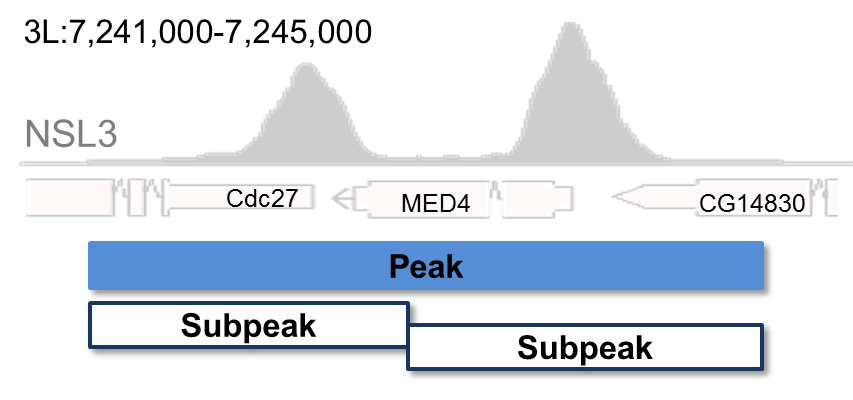
\includegraphics[width=6.5cm,trim=2 2 2 2,clip]{Figures/PeakCalling_Dmel}}
				\end{minipage} 
%\\ [2ex]  \hline \\ [1ex]
\tabularnewline \midrule
%-----------------------
\begin{minipage}[c]{3.5cm}
Pol~II in\\\textit{D.~melanogaster} cells\\(depleted of NSL1 or NSL3)
\end{minipage}
	& \begin{minipage}[c]{4cm}
	the mixed signal of Pol~II (localized, TF-like enrichments around TSS, broad, shallow enrichments along gene bodies) was not well captured by MACS
		\end{minipage}
		& \begin{minipage}[c]{8cm}
\vskip 6pt
				\begin{enumerate}[noitemsep, leftmargin=*]
					\item a symmetric null distribution was fitted to regions with negative enrichments, i.e. where the input signal exceeded the ChIP signal \citep{EBIroutine} (black line)
					\item genomic bins that deviated from the expectation (compare the blue with the black line) were determined as significantly enriched (threshold: q-value $\leq$ 0.05) \\ [2ex]
				\end{enumerate}
\vskip 4pt
			\end{minipage}
				& \begin{minipage}[c]{6.5cm}
						\parbox[c]{1em}{
						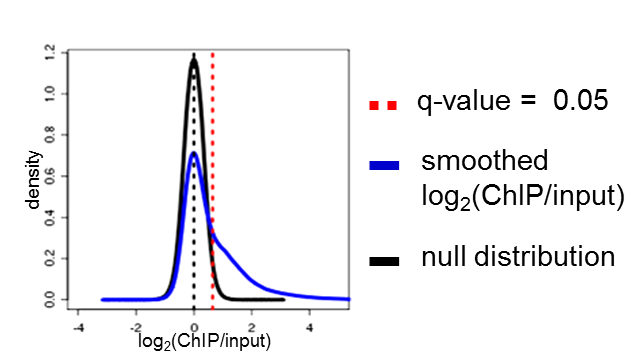
\includegraphics[width=6.5cm,trim=4 4 4 4,clip]{Figures/PeakCalling_PolII}}
					\end{minipage}
%\\ [2ex] \hline \\ [1ex]
\tabularnewline \midrule
%-----------------------
\begin{minipage}[c]{3.5cm}
MOF, MSL1, MSL2,\\NSL3, MCRS1 in\\ mouse ESCs and NPCs
\end{minipage}
	& \begin{minipage}[c]{4cm}
	non-optimal signal-noise ratios, GC bias
		\end{minipage}
		& \begin{minipage}[c]{8cm}
\vskip 6pt
				\begin{enumerate}[noitemsep, leftmargin=*]
                    \item in ESCs: adjustment of the GC bias in the input sample to match each ChIP-seq sample's GC bias
					\item peak calling with MACS 1.4.2 with default parameters \citep{Feng2012} for each ChIP-seq replicate (blue boxes) and the merged file (red box)
					\item only peaks that were present in both replicates and met the FDR threshold of $\leq$ 1\% were used \\ [2ex]
				\end{enumerate}
\vskip 4pt
			\end{minipage}
				& \begin{minipage}[c]{6.5cm}
\vskip 6pt
						\parbox[c]{1em}{
						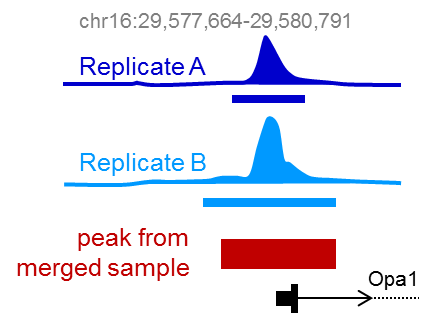
\includegraphics[width=5.5cm,trim=4 4 4 4,clip]{Figures/PeakCalling_Mm}} 
\vskip 4pt
					\end{minipage}
%\\ [2ex] \hline \\ [1ex]
%-----------------------
\tabularnewline \bottomrule
\label{tab:peakCallingStrategies}
\end{longtable}
\end{small}
\end{singlespacing}
\end{landscape}
%
\subsection{Datasets}
\label{Datasets}
All analyses were enriched by the integration of previously published, publicly available high-throughput sequencing data and annotation.\\
%
\begin{minipage}{\textwidth} % to avoid pagebreaks despite longtable environment
\begin{singlespacing}
\begin{small}
\setlength{\extrarowheight}{2pt}
%\vspace*{-2em}
\begin{longtable}[l]{>{\textsf\bgroup}p{2cm}<{\egroup} >{\textsf\bgroup}p{6cm}<{\egroup} >{\textsf\bgroup}p{6cm}<{\egroup}} % defining the columns - these must match the widths defined for the mini pages down below!
\caption[Publicly available data bases that were used.]{\textsf{Publicly available data bases that were used.}} \\ % the \\ is important!
%%%%%%%%%%%%%%%
% table title
\textbf{Name} & \textbf{Application} & \textbf{Website}
\tabularnewline
%-----------------------
\toprule
 ArrayExpress & up- and download of high-throughput sequencing data (only raw read files) & \url{http://www.ebi.ac.uk/arrayexpress/} 
\tabularnewline \midrule
%--------------------------
 BioMart & mapping of gene and transcripts between different annotations for genome version mm9, e.g. Ensembl and RefSeq; download of non-protein-coding transcripts & \url{http://may2012.archive.ensembl.org/biomart/martview/} 
\tabularnewline \midrule
%--------------------------
 FlyBase & download of gene lists and genome sequence & \url{http://flybase.org/} 
\tabularnewline \midrule
%--------------------------
GEO & up- and download of high-throughput sequencing data (raw and processed data) & \url{http://www.ncbi.nlm.nih.gov/geo/} 
\tabularnewline \midrule
%--------------------------
HomoloGene & list of orthologous genes in \textit{Drosophila}, mice and humans & \url{http://www.ncbi.nlm.nih.gov/homologene} 
\tabularnewline \midrule
%--------------------------
\raggedright UCSC Table Browser & RefSeq gene lists, mappability tracks, GC content tracks, mouse DNase hypersensitivity tracks & \url{https://genome.ucsc.edu/}
%--------------------------
\tabularnewline \bottomrule
%-----------------------------
\label{tab:DB}
\end{longtable}
\end{small}
\end{singlespacing}
\end{minipage}

%
All samples generated by members of the Akhtar lab were uploaded to public repositories. Accession numbers starting with G indicate the GEO database, accession numbers starting with E indicate ArrayExpress (see \tref{tab:DB}). The DNA read numbers are based on filtered reads. Read and accession numbers refer to all available replicates of each experiment.
%
\subsubsection{\textit{Drosophila} datasets}
%
The subsequently listed data was used for Lam, Mühlpfordt, Vaquerizas et al. \citep{Lam2012} (\aref{SuppPub_NSL}) and Chlamydas et al.\\
\begin{singlespacing}
\begin{small}
\begin{sffamily}
\vspace*{-2em}
\begin{longtable}[l]{p{2.3cm}p{2.5cm}p{3.5cm}p{2cm}p{3cm}}
\caption[In-house generated ChIP-seq samples from \textit{D.~melanogaster} larva and Schneider S2 cells.]{\textsf{In-house generated ChIP-seq samples from \textit{D.~melanogaster} larva and cell culture (Schneider S2 cells \citep{Schneider1972}).}} \\
%%%%%%%%%%%%%%%%%%%%%%%%%%%%%%%%%%%%%%%%%
% table title
\textbf{Sample} & \textbf{Generated by} & \textbf{Cells/Tissue} & \textbf{Reads ($\times 10^6$)} & \textbf{Accession number}
\tabularnewline \toprule
\endfirsthead % indicates that the lines above appear as head of the table on the first page
%
\multicolumn{5}{c}%
{\tablename\ \thetable\ -- \textit{Continued from previous page}} \\[1ex]
\textbf{Sample} & \textbf{Generated by} & \textbf{Cells/Tissue} & \textbf{Reads ($\times 10^6$)} & \textbf{Accession number}
\tabularnewline \toprule %\tabularnewline %[1ex]
\endhead % Line(s) to appear at top of every page (except first)
%
\hline \multicolumn{5}{r}{\textit{Continued on next page}} \\
\endfoot % Last line(s) to appear at the bottom of every page (except last)
\endlastfoot
%%%%%%%%%%%%%%%%%%%%%%%%%%
%\tabularnewline \toprule
Input & Sunil J. Raja & \raggedright larval salivary glands & 6.1 & E-MTAB-214
\tabularnewline \midrule
NSL1 	& Sunil J. Raja & \raggedright larval salivary glands  & 7.6 & E-MTAB-214
\tabularnewline \midrule
MCRS2 & Sunil J. Raja & \raggedright larval salivary glands  & 9.4 & E-MTAB-214
\tabularnewline \midrule
Input & Ibrahim Ilik & S2 cells & 21.2	& E-MTAB-1085
\tabularnewline \midrule
NSL3 	& Kin C. Lam & S2 cells & 28.3  	& E-MTAB-1085
\tabularnewline \midrule
MBD-R2 & Kin C. Lam & S2 cells & 27.3 	& E-MTAB-1085
\tabularnewline \midrule
Input & Kin C. Lam & \raggedright S2 cells (NSL1~RNAi) & 47.1 & E-MTAB-1084
\tabularnewline \midrule
Pol II (Rbp3) & Kin C. Lam & \raggedright S2 cells (NSL1~RNAi) & 132; 132.1 & E-MTAB-1084
\tabularnewline \midrule
Input & Kin C. Lam & \raggedright S2 cells (NSL3~RNAi) & 57.2 & E-MTAB-1084
\tabularnewline \midrule
Pol II (Rbp3) & Kin C. Lam & \raggedright S2 cells (NSL3~RNAi) & 120; 134.9 & E-MTAB-1084
\tabularnewline \midrule
Input & Kin C. Lam & \raggedright S2 cells (GFP~RNAi) & 50; 60 & E-MTAB-1084
\tabularnewline \midrule
Pol II (Rbp3) & Kin C. Lam & \raggedright S2 cells (GFP~RNAi) & 134 & E-MTAB-1084
\tabularnewline \midrule
Input & Thomas Conrad & \raggedright larval salivary glands (females) & 14.8 & E-MTAB-911 
\tabularnewline \midrule
Input & Thomas Conrad & \raggedright larval salivary glands (males) & 6.6 & E-MTAB-911 
\tabularnewline \midrule
H4K16ac & Thomas Conrad & \raggedright larval salivary glands (females) & 11.8 & E-MTAB-911
\tabularnewline \midrule
H4K16ac & Thomas Conrad & \raggedright larval salivary glands (males) & 9.4 & E-MTAB-911
\tabularnewline \midrule
MOF & Thomas Conrad & \raggedright larval salivary glands (females) & 7.5 & E-MTAB-911
\tabularnewline \midrule
MOF & Thomas Conrad & \raggedright larval salivary glands (males) & 9.2 & E-MTAB-911
\tabularnewline \midrule
MSL1 & Thomas Conrad & \raggedright larval salivary glands (males) & 6.7 & GSM1502677
\tabularnewline \midrule
MSL1 & Sunil J. Raja & \raggedright larval salivary glands (females) & 10.7 & GSM1502675
%%%%%%%%%%%%%%%%%%%%%%%%%%%%
\tabularnewline \bottomrule
\label{tab:ChIPseqSamplesDmel}
%%%%%%%%%%%%%%%%%%%%%%%%%%%%%%
\end{longtable}
%
\begin{minipage}{\textwidth}
\vspace*{-2em}
\begin{longtable}{p{1.5cm}p{3.5cm}p{3.5cm}p{2cm}p{3cm}}
\caption[In-house generated ChIP-seq samples from \textit{D.~virilis} larva that were used for Chlamydas et al.]{\textsf{In-house generated ChIP-seq samples from \textit{D.~virilis} larva that were used for Chlamydas et al. (\aref{SuppPub_MSL1})}} \\
%%%%%%%%%%%%%%%%%%%%%%%%%%%%%%%%%%%%%%%%%
% table title
\textbf{Sample} & \textbf{Generated by} & \textbf{Cells/Tissue} & \textbf{Reads ($\times 10^6$)} & \textbf{Accession number}
\tabularnewline \toprule
%%%%%%%%%%%%%%%%%%%%%%%%%%
%\tabularnewline \toprule
Input & Sarantis Chlamydas & \raggedright larval salivary glands (females) & 224.3; 230 & GSM1502682, GSM1502684
\tabularnewline \midrule
MSL1 & Sarantis Chlamydas & \raggedright larval salivary glands (males) & 210; 225 & GSM1502681, GSM1502683
%%%%%%%%%%%%%%%%%%%%%%%%%%%%
\tabularnewline \bottomrule
\label{tab:ChIPseqSamplesDvir}
%%%%%%%%%%%%%%%%%%%%%%%%%%%%%%
\end{longtable}
\end{minipage}
%
\end{sffamily}
\end{small}
\end{singlespacing}

\clearpage
% TABLE: Public (non-in-house) data sets
\begin{singlespacing}
\begin{small}
\begin{sffamily}
\vspace*{-2em}
\begin{longtable}[l]{p{2.5cm}p{3.2cm}p{3cm}}
\caption[ChIP-chip modENCODE data sets from S2 cells.]{\textsf{ChIP-chip modENCODE data sets for which we downloaded the processed coverage files from GEO. All ChIP experiments were done in S2 cells.}} \\
%%%%%%%%%%%%%%%%%%%%%%%%%%%%%%%%%%%%%%%%%
% table title
\textbf{Sample} & \textbf{Downloaded data} & \textbf{Accession number} 
\tabularnewline \toprule
\endfirsthead % indicates that the lines above appear as head of the table on the first page
%
\multicolumn{3}{c}%
{\tablename\ \thetable\ -- \textit{Continued from previous page}} \\
\textbf{Sample} & \textbf{Downloaded data} & \textbf{Source} 
\tabularnewline \toprule \tabularnewline [1ex]
\endhead % Line(s) to appear at top of every page (except first)
%
\hline \multicolumn{3}{r}{\textit{Continued on next page}} \\
\endfoot % Last line(s) to appear at the bottom of every page (except last)
\endlastfoot
%%%%%%%%%%%%%%%%%%%%%%%%%%
%\tabularnewline \toprule
H3 & .bedgraph & GSM93208
\tabularnewline \midrule
%
H3K4me3 & .bedgraph & GSE20787
\tabularnewline \midrule
H3K36me3 & .bedgraph & GSE20785
\tabularnewline \midrule
H3K4me2 & .bedgraph & GSE23470
\tabularnewline \midrule
H4K5ac & .bedgraph & GSE20800
\tabularnewline \midrule
H3K9ac & .bedgraph & GSE20790
\tabularnewline \midrule
H4K8ac & .bedgraph & GSE20801
\tabularnewline \midrule
H3K9me3 & .bedgraph & GSE20794
\tabularnewline \midrule
H3K9me3 & .bedgraph & GSE20794
%%%%%%%%%%%%%%%%%%%%%%%%%%%
\tabularnewline \bottomrule
\label{tab:modENCODE}
%%%%%%%%%%%%%%%%%%%%%%%%%%%%%%
\end{longtable}
%
\vspace{-2em}
%
\begin{minipage}{\textwidth}
\begin{longtable}[l]{p{2.5cm}p{3.2cm}p{3cm}}
\caption[Publicly available ChIP-seq data of MSL complex members in \textit{Drosophila}.]{\textsf{ChIP-seq data of MSL complex members, downloaded and processed by Fidel Ramírez and used for \fref{fig:profiles}.}} \\
%%%%%%%%%%%%%%%%%%%%%%%%%%%%%%%%%%%%%%%%%
% table title
\textbf{Sample} & \textbf{Accession number} 
\tabularnewline \toprule
MSL2 & GSE37864
\tabularnewline \midrule
MSL3 & GSE37864
\tabularnewline \midrule
MLE & SRX111555
\tabularnewline \bottomrule
\label{tab:Becker}
%%%%%%%%%%%%%%%%%%%%%%%%%%%%%%
\end{longtable}
\end{minipage}
\end{sffamily}
\end{small}
\end{singlespacing}


%%%%%%%%%%%%%%%%%%%%%%%%%%%%%%%%%%%%
\subsubsection{Mouse datasets}
The following data was used for Chelmicki, Dündar et al.\citep{Chelmicki2014} (\aref{SuppPub_MSL}). MSL1 and input samples were also used for Chlamydas et al. (\aref{SuppPub_MSL1}). \\
%\begin{landscape}
\begin{singlespacing}
\begin{small}
\begin{sffamily}
%\setlength{\extrarowheight}{15pt} % this doesn't work to control the vertical space
\vspace*{-2em}
\begin{longtable}[l]{p{1.5cm}p{3.2cm}p{2cm}p{2cm}p{4.3cm}} % defining the columns 
\caption[In-house generated ChIP-seq samples from mESC and mNPC.]{\textsf{ChIP-seq samples from murine embryonic stem cells (mESC) and neuronal progenitor cells (mNPC) generated by Tomasz Chelmicki and the Deep Sequencing Facility at the Max Planck Institute of Immunobiology and Epigenetics.}} \\ % the \\ is important! 
%%%%%%%%%%%%%%%
% table title
\textbf{Sample} & \textbf{Generated by} & \textbf{Cells/Tissue} & \textbf{Reads ($\times 10^6$)} & \textbf{Accession number}
\tabularnewline \hline
\endfirsthead % indicates that the lines above appear as head of the table on the first page
%
\multicolumn{4}{c}%
{\tablename\ \thetable\ -- \textit{Continued from previous page}} \\[1ex]
\textbf{Sample} & \textbf{Generated by} & \textbf{Cells/Tissue} & \textbf{Reads ($\times 10^6$)} & \textbf{Accession number}
\tabularnewline \toprule %\tabularnewline [1ex]
\endhead % Line(s) to appear at top of every page (except first)
%
\multicolumn{4}{r}{\textit{Continued on next page}} \\
\endfoot % Last line(s) to appear at the bottom of every page (except last)
\endlastfoot
%%%%%%%%%%%%%%%%%%%
%% first row
%-----------------------
Input & Tomasz Chelmicki & mESC & 62; 27 & GSM1251941, GSM1251942
\tabularnewline \midrule
MOF & Tomasz Chelmicki & mESC & 23.3; 34.9 & GSM1251945, GSM1251946
\tabularnewline \midrule
MSL1 & Tomasz Chelmicki & mESC & 28.3; 20.3 & GSM1251947, GSM1251948
\tabularnewline \midrule
MSL2 & Tomasz Chelmicki & mESC & 15.8; 11 & GSM1251949, GSM1251950
\tabularnewline \midrule
KANSL3 & Tomasz Chelmicki & mESC & 21.6; 15.3 & GSM1251951, GSM1251952
\tabularnewline \midrule
MCRS1 & Tomasz Chelmicki & mESC & 19.7; 20.7 & GSM1251943, GSM1251944
\tabularnewline \midrule
Input & Tomasz Chelmicki & mNPC & 106; 102 & GSM1251953, GSM1251954
\tabularnewline \midrule
MOF & Tomasz Chelmicki & mNPC & 65; 75 & GSM1251955, GSM1251956
\tabularnewline \midrule
MSL2 & Tomasz Chelmicki & mNPC & 116; 112 & GSM1251957, GSM1251958
\tabularnewline \midrule
KANSL3 & Tomasz Chelmicki & mNPC & 82.8; 93.6 & GSM1251957, GSM1251960
\tabularnewline \bottomrule
%-----------------------------
\label{tab:ChIPseqSamplesMM}
\end{longtable}
\end{sffamily}
\end{small}
\end{singlespacing}
%\end{landscape}

\input{Tables/Table_RNASeqSamples}
\begin{singlespacing}
\begin{small}
\begin{sffamily}
\vspace*{-2em}
\begin{longtable}[l]{p{4.3cm}p{3.2cm}p{6.5cm}}
%%%%%%%%%%%%%%%%%%%%%%%%%%%
\caption[Publicly available mouse data sets and annotation.]{\textsf{Publicly available mouse data sets and annotation that were used for Chelmicki, Dündar et al.\citep{Chelmicki2014} (\aref{SuppPub_MSL})}} \\
%%%%%%%%%%%%%%%%%%%%%%%%%%%
\textbf{Sample} & \textbf{Downloaded data} & \textbf{Source} 
\tabularnewline \toprule
\endfirsthead % indicates that the lines above appear as head of the table on the first page
%
\multicolumn{3}{c}%
{\tablename\ \thetable\ -- \textit{Continued from previous page}} \\[1ex]
\textbf{Sample} & \textbf{Downloaded data} & \textbf{Source} 
%\tabularnewline \toprule %\tabularnewline [1ex]
\endhead % Line(s) to appear at top of every page (except first)
%
\hline \multicolumn{3}{r}{\textit{Continued on next page}} \\
\endfoot % Last line(s) to appear at the bottom of every page (except last)
\endlastfoot
%%%%%%%%%%%%%%%%%%%%%%%%%%%
Enhancers defined by histone marks & .bed-file of peaks & supplement of \citet{Creyghton2010}
\tabularnewline \midrule
%-----------------------
Super/typical enhancers & .bed-file of regions & supplement of \citet{Whyte2013}
\tabularnewline \midrule
%-----------------------
RNA Pol II ChIP-seq (mESC) & .wig-file of signal & GSM632040
\tabularnewline \midrule
%-----------------------
RNA Pol II ChIP-seq (mNPC) & .wig-file of signal & GSM632050
\tabularnewline \midrule
%-----------------------
p300 ChIP-seq (mESC) & .wig-file of signal & GSM723018
\tabularnewline \midrule
%-----------------------
H3K4me1 ChIP-seq (mESC) & .wig-file of signal & GSM723016
\tabularnewline \midrule
%-----------------------
H3K27ac ChIP-seq (mESC) & FASTQ file & GSM1005503
\tabularnewline \midrule
%-----------------------
CpG methylation (mESC) & .tsv-file of counts & GSE30202
\tabularnewline \midrule
%-----------------------
CpG methylation (mNPC) & .tsv-file of counts & GSE30202
\tabularnewline \midrule
%-----------------------
\raggedright DNase hypersensitivity (mESC) & .wig-file of signal & \raggedright from the UCSC Genome~Browser: wgEncodeUwDnaseEscj7S129ME0SigRep1
\tabularnewline \bottomrule
%-----------------------
\label{tab:PublicSamplesMM}
\end{longtable} 
\end{sffamily}
\end{small}
\end{singlespacing}

%%%%%%%%%%%%%%%%%%%%%%%%%%%%%

\chapter{Academic vita}
\begin{singlespacing}
\vspace*{-1cm}
\textbf{\Large{Education}}
\begin{singlespacing}
%\begin{small}
%\setlength{\extrarowheight}{1.5pt}
\vspace*{-1em}
\begin{longtable}[l]{p{6cm}p{8cm}} % defining the columns 
%-----------------------
\raggedright since May 2011 PhD Candidate &
International Max Planck Research School for Molecular and Cellular Biology, Faculty of Biology, University of Freiburg
\tabularnewline  [0.3cm]
%----------------
\begin{minipage}[t]{6cm}
\raggedright 2010 Master of Science\\ \hspace{0.8cm} (Biomedicine)
\end{minipage}  & 
\begin{minipage}[t]{8cm}
University of Würzburg\\
\raggedright Thesis: \textit{Molecular Studies on BAR domain proteins in murine hematopoietic cells}
\end{minipage}
\tabularnewline [1.3cm]
%----------------
\begin{minipage}[t]{6cm}
\raggedright 2008 Bachelor of Science \\ \hspace{0.8cm} (Biomedicine)
\end{minipage}
&
\begin{minipage}[t]{8cm}
University of Würzburg \\
\raggedright Thesis: \textit{Effects of NAD(P)H Oxidase Inhibitors on Thrombocyte Function and Haemostasis}
\end{minipage}
\tabularnewline [1.3cm]
%----------------
\raggedright 2006-2011 Stipend & German National Merit Foundation
\tabularnewline [0.3cm]
%----------------
\raggedright 2005 Abitur & Neideck Gymnasium Arnstadt
\tabularnewline [0.3cm]
%----------------
\raggedright 2003 High School Diploma & Vallivue High School, Caldwell, ID, USA
\tabularnewline [0.3cm]
%----------------
\raggedright 2002 Ober\-stufen\-ab\-schluss\\ \hspace{0.8cm} Kammermusik   & Kreismusikschule Arnstadt-Ilmenau
\tabularnewline
\end{longtable}
%\end{small}
\end{singlespacing}
\vspace*{0.2cm}
\textbf{\Large{Publications}}

Chelmicki T and \textbf{D{\"u}ndar F}* et al. MOF complexes use short and long-range interactions to ensure stem cell identity and Xist repression. \textit{eLife} 2014 May 19;3:e02024.

Ramirez F and \textbf{D{\"u}ndar F}* et al. deepTools: Analyzing and visualizing high-throughput sequencing data. \textit{Nucleic Acids Research} 2014 Jul;42(Web Server issue):W187-91.

Lam KC, \textbf{M{\"u}hlpfordt F}* and Vaquerizas JM et al. The NSL complex regulates housekeeping genes in Drosophila. \textit{PLoS Genetics} 2012 May;8(6):e1002736. 

Bobak N et al.** Volume regulation of murine T lymphocytes relies on voltage-dependent and two-pore domain potassium channels. \textit{Biochim Biophys Acta.} 2011 Aug;1808(8):2036-44.

* shared first authorship, ** author on 5th position
\end{singlespacing}

\addtocontents{toc}{\vspace{2em}} % Add a gap in the Contents, for aesthetics

\backmatter

%----------------------------------------------------------------------------------------
%	BIBLIOGRAPHY
%----------------------------------------------------------------------------------------

\label{Bibliography}

%\lhead{\emph{References}} % Change the page header to say "References"
\fancyhead[RO,LE]{Bibliography}
\fancyfoot[C]{\thepage}

\begin{singlespacing}
\begin{sffamily}
\begin{footnotesize}
\bibliographystyle{MYunsrtnat} % Use the "unsrtnat" BibTeX style for formatting the Bibliography
\setlength{\bibsep}{2pt}
\bibliography{BibliographyMod} % The references (bibliography) information are stored in the file named "Bibliography.bib"
\end{footnotesize}
\end{sffamily}
\end{singlespacing}

\end{document}  

